        
\documentclass[12pt]{book}
\usepackage{graphicx,ae}
\usepackage{color}
\usepackage{amsmath}
\usepackage{amssymb}
\usepackage{hyperref}
\usepackage{fullpage}


%
% this command enables to remove a whole part of the text
% from the printout
% to use it just enter
% \remove{
% before the text to be excluded and
% }
% after the text
\newcommand{\remove}[1]{}
%
% The following macros are used to generate nice code for programs.
% See example on how to use it below
%
%%%%%%%%%%%%%%%%%%%%% program macros %%%%%%%%%%%%%%%%%
\newcommand{\Do}{{\small\bf do}\ }
\newcommand{\Return}{{\small\bf return\ }}
\newcommand{\Proc}[1]{#1\+}
\newcommand{\Returns}{{\small\bf returns}}
\newcommand{\Procbegin}{{\small\bf begin}}
\newcommand{\If}{{\small\bf if}\ \=\+}
\newcommand{\Then}{{\small\bf then}\ \=\+}
\newcommand{\Else}{\<{\small\bf else}\ \>}
\newcommand{\Elseif}{\<{\small\bf elseif}\ }
\newcommand{\Endif}{\<{\small\bf end\ if\ }\-\-}
\newcommand{\Endproc}[1]{{\small\bf end} #1\-}
\newcommand{\For}{{\small\bf for}\ \=\+}
\newcommand{\Endfor}{{\small\bf end\ for}\ \-}
\newcommand{\Loop}{{\bf loop}\ \= \+}
\newcommand{\Endloop}{{\bf end\ loop}\ \-}
\newenvironment{program}{
    \begin{minipage}{\textwidth}
    \begin{tabbing}
    \ \ \ \ \=\kill
  }{
    \end{tabbing}
    \end{minipage}
  }

%
\newcommand{\topic}[2]{\section{#1} \index{#2} \markright{#1}}
\newcommand{\subtopic}[2]{\subsection{#1} \index{#2}}
\newcommand{\subsubtopic}[2]{\subsubsection{#1} \index{#2}}


\usepackage{framed}

\newcommand{\ymignore}[1]{}

%\documentclass[11pt]{report}
\usepackage{geometry}                % See geometry.pdf to learn the layout options. There are lots.
%\geometry{letterpaper}                   % ... or a4paper or a5paper or ...
%\geometry{landscape}                % Activate for for rotated page geometry
%\usepackage[parfill]{parskip}    % Activate to begin paragraphs with an empty line rather than an indent
\usepackage{graphicx}
\usepackage{amssymb}
\usepackage{epstopdf}
\usepackage{amsfonts}
\usepackage{amsthm}
\usepackage{amsmath}
\usepackage{tikz}
\usepackage{algorithm2e}
% \usepackage{algorithm}
\usepackage{algorithmic}
\usepackage{url}
\usepackage{comment}
\usepackage{color}

\newcommand{\mdp}{\mathcal{M}}
\newcommand{\Mdp}{\mathcal{M}}
\newcommand{\Agent}{\mathcal{G}}
\newcommand{\env}{\mdp}
\newcommand{\Env}{\mdp}

\newcommand{\Actions}{\mathcal{A}}
\newcommand{\action}{{\tt a}}
\newcommand{\actionp}{a^{\prime}}
\newcommand{\actionpp}{a^{\prime\prime}}

\newcommand{\States}{\mathcal{S}}
\newcommand{\state}{{\tt s}}
\newcommand{\statep}{\state^{\prime}}
\newcommand{\statepp}{\state^{\prime\prime}}
\newcommand{\eststate}{x}

\newcommand{\transitionprob}{{\tt p}}


\newcommand{\ttime}{{\tt t}}
\newcommand{\tHorizon}{{\tt T}}

\newcommand{\weight}{{\tt w}}

\newcommand{\spath}{{\tt \omega}}
\newcommand{\edge}{{\tt e}}
\newcommand{\edges}{{\tt E}}
\newcommand{\node}{{\tt v}}
\newcommand{\nodeu}{{\tt u}}
\newcommand{\nodev}{{\tt v}}
\newcommand{\nodes}{{\tt V}}
\newcommand{\graph}{{\tt G}}
\newcommand{\minlen}{{\tt d}}
\newcommand{\pathlen}{{\tt c}}
\newcommand{\vertexset}{{S}}
\newcommand{\queue}{{Q}}
\newcommand{\heur}{{\tt h}}

\newcommand{\observation}{{\tt o}}
\newcommand{\fObservation}{\mathcal{O}}

\newcommand{\thistory}{{\tt h}}
\newcommand{\Cost}{\mathcal{C}}
\newcommand{\cost}{{\tt c}}
%\newcommand{\Value}{V}
%\newcommand{\reward}{r}
\newcommand{\discount}{\gamma}
\newcommand{\Rmax}{{\tt R}_{\max }}
\newcommand{\Vmax}{{\tt V}_{\max }}



\newcommand{\la}{\lambda}
\newcommand{\om}{\omega}
\newcommand{\ga}{\gamma}
\newcommand{\al}{\alpha}
\newcommand{\eps}{\epsilon}
\newcommand{\dfn}{\triangleq}
\newcommand{\cF}{\mathcal F}
\newcommand{\cX}{\mathcal X}
\newcommand{\negspace}{\!}
\newcommand{\obs}{o}
\newcommand{\Obs}{\mathcal{O}}
\newcommand{\reward}{{\tt r}}
\newcommand{\terminalreward}{r^T}
\newcommand{\rew}{\reward}
\newcommand{\Rewards}{{\tt R}} %
\newcommand{\history}{{\tt h}} %
\newcommand{\histories}{\mathcal{H}}
\newcommand{\Histories}{\mathcal{H}}
\newcommand{\Trans}{T}
\newcommand{\Horizon}{t_f}
\newcommand{\TUtility}{U_T}
\newcommand{\Utility}{U_{\gamma}}
\newcommand{\AUtility}{U_A}
\newcommand{\TValue}{J}
\newcommand{\TAValue}{K}
\newcommand{\Value}{\mathcal{V}} %
\newcommand{\Valuepi}{V^\policy} %
\newcommand{\QValue}{\mathcal{Q}} %


\newcommand{\operator}{\mathcal{T}}

\newcommand{\hatValue}{{\widehat{V}}}
\newcommand{\AValue}{Q}
\newcommand{\hatAValue}{{\widehat{Q}}}
\newcommand{\AvgRValue}{\rho}
\newcommand{\hatAvgRValue}{{\widehat{\rho}}}
\newcommand{\RelValue}{W}
\newcommand{\hatRelValue}{{\widehat{W}}}

\newcommand{\stateestfunction}{f_{su}}
\newcommand{\stateobsfunction}{f_{so}}
\newcommand{\statetransfunction}{f_{ss}}
\newcommand{\rewfunction}{f_r}
\newcommand{\field}[1]{\mathbb{#1}}
\newcommand{\Reals}{\field{R}}
%\newcommand{\eqref}[1]{(\ref{#1})}
\newcommand{\policy}{\pi}
\newcommand{\hatpolicy}{{\widehat{\pi}}}
\newcommand{\Policies}{\Pi}
\newcommand{\nspolicy}{\mu}
\newcommand{\norm}[1]{\| {#1} \|}

\newcommand{\union}{\ensuremath{\bigcup}}
\newcommand{\comps}{\ensuremath{\mathbb{C}}}
\newcommand{\reals}{\ensuremath{\mathbb{R}}}
\newcommand{\Var}{\ensuremath{\mathrm{Var}}}
\newcommand{\var}{\ensuremath{\mathrm{Var}}}
\newcommand{\E}{\ensuremath{\mathbb{E}}}
\renewcommand{\P}{\ensuremath{\mathbb{P}}}
\newcommand{\R}{\ensuremath{\mathbb{R}}}
\newcommand{\T}{\ensuremath{\mathbb{T}}}
\newcommand{\Z}{\ensuremath{\mathbb{Z}}}
\newcommand{\I}{\ensuremath{\mathbb{I}}}


\newcommand{\mixtime}{\tau}
\newcommand{\epshorizon}{\tau}

\def\argmax{\operatornamewithlimits{arg\,max}}
\def\argmin{\operatornamewithlimits{arg\,min}}

\newcommand{\bydef}{\stackrel{\bigtriangleup}{=}}
\newcommand\defeq{\stackrel{\mathrm{def}}{=}}
\newcommand{\half}{\frac{1}{2}}

\newcommand{\coderemark}[1]{\textcolor{blue}{\% #1}}
\newcommand{\itab}[1]{\hspace{0em}\rlap{#1}}
\newcommand{\tab}[1]{\hspace{1em}\rlap{#1}}

\DeclareGraphicsRule{.tif}{png}{.png}{`convert #1 `dirname #1`/`basename #1 .tif`.png}

%\newtheorem{theorem}{Theorem}[chapter]
\newtheorem{theorem}{Theorem}
\numberwithin{theorem}{chapter}
\newtheorem*{theorem*}{Theorem}
\newtheorem{lemma}[theorem]{Lemma}
%\numberwithin{lemma}{chapter}
\newtheorem{proposition}[theorem]{Proposition}
%\numberwithin{proposition}{chapter}
\newtheorem{corollary}[theorem]{Corollary}
%\numberwithin{corollary}{chapter}
\newtheorem{assumption}{Assumption}
\numberwithin{assumption}{chapter}
\newtheorem{definition}{Definition}
\numberwithin{definition}{chapter}
\newtheorem{example}{Example}
\numberwithin{example}{chapter}
\newtheorem{claim}[theorem]{Claim}
%\numberwithin{claim}{chapter}

\newtheorem{exercise}{Exercise}
\numberwithin{exercise}{chapter}
% no italics in exercise
%YM: commented
%\usepackage{xparse}
%\let\oldexercise\exercise
%\RenewDocumentCommand{\exercise}{o}{%
%  \IfNoValueTF{#1}
%    {\oldexercise}
%    {\oldexercise[#1]}%
%  \normalfont
%}
\newtheorem{remark}{Remark}
\numberwithin{remark}{chapter}
\newtheorem{algorithm_}{Algorithm}
\numberwithin{algorithm_}{chapter}



\title{Reinforcement Learning: Foundations}
\date{February 2021}                                           % Activate to display a given date or no date
\author{Shie Mannor, Yishay Mansour and Aviv Tamar}

\begin{document}
\maketitle

% \tableofcontents

% \chapter{Introduction and Overview}
% \label{chapter:intro}
% \section{What is RL?}

Concisely defined, Reinforcement Learning, abbreviated as RL, is the discipline of learning and acting in 
environments where sequential decisions are made. That is, the decision made at a given time 
will be followed by other decisions and therefore the decision maker has to consider the implications 
of her decision.

In the early days of the field, there was an analogy drawn between human learning and computer 
learning. While the two are certainly tightly connected, this is merely an analogy that serves to motivate and inspire. Other terms that 
have been used are approximate dynamic programming (ADP), neuro-dynamic programming (NDP), which to us
mean the same thing, but focus on a specific collection of techniques that came to be known as ``RL''.

 \medskip
\noindent{\it Origins of reinforcement learning}
%
Reinforcement learning spans a large number of disciplines.
Naturally, by our own indoctrination, we are going to look through the lens of Computer Science
and Machine Learning. From an engineering perspective, optimal control is 
the ``mother'' of RL with many of the concepts that are used in RL naturally come from optimal control. 
Other notable origins are in Operation Research, where the initial mathematical works have originated.
Addition disciplines include: Neuroscience, Psychology, Statistics and
Economics.

The origins of the term ``reinforcement learning'' is in psychology, where it refers to learning by trail and error. 
While this inspired much work in the early days of the field, current approaches are mostly based on
machine learning an optimal control. We refer the reader to Section 1.6 in \cite{book:Sutton} for an
a detailed history of RL as a field. 

\section{Motivation for RL}

In the recent years there is a renewed interest in RL. The new interest is grounded in  emerging applications
of RL, and also in much progress in the field of deep learning that
has been impressively applied for solving challenging RL tasks. 
But for us, the interest comes from the {\em promise} of RL and its
potential to be an effective tool for control and behavior in dynamic environments.

Over the years reinforcement learning has proven to be highly
successful for playing board games over a long history. Gerald
Tesauro in 1992 developed the TD-gammon \cite{XX}, which uses a two layer
neural-network to achieve a high performance backgammon computer
game. The network was trained by bootstrapping it from scratch and
learned a temporal differences function. One of the amazing features
of the TD-gammon was that even in the {\em first} move, it used a
different game move than the grandmasters, who later adopted the new
game move once they observe TD-gammon playing it \cite{XX}.

Recently, Deep Mind have developed a deep neural-network
to play Go, which is able to beat the best Go players in the world.
Developing a human-level computer Go program has been a challenge
that has persisted for decades.
Early in 1962, Arthur Samuel developed a checkers game, which was at
the level of the best human. His original framework included many of
the ingredients which latter contributed to RL,
as well as search heuristic for large domains.

To complete the picture of computer board games, we should mention
Deep Blue, from 1996, which was able to beat the world champion then,
Kasparov. This program was mainly built on a heuristic search, and
developed a new simple hardware to support it. Recently, Deep Mind
came out with a deep neural-network that matched the best chess
programs (which are already much better than any human players).

Another domain, popularized by DeepMind, is playing Atari video
games \cite{XX}, which where popular in the 1980's. DeepMind were able to
show how deep neural networks can achieve human level performance,
using only the video picture as input (and having no additional
information about the goal of the game). There has been many successes in games
such Starcraft\cite{xx}, Dotta \cite{xx}, and others.

Looking in to the future, the real promise of RL
is learning in interactive settings. Probably one the most important
applications is robotics, where reaching a human level performance
would have far outreaching consequences.



\medskip
\noindent{\it Mathematical Model}
%
The main mathematical model we will use is Markov Decision Process
(MDP). The model tries to capture uncertainty in the dynamics of the
environment, the actions and our knowledge. The main focus would be
on decision making, namely, selecting actions. The evaluation would
consider the long term effect of the actions, trading-off immediate
rewards with long-term gains.

In contrast to Machine Learning, the reinforcement learning model
would have a {\em state}, and the algorithm will influence the state
through its actions.
% distribution (as well as the immediate observed rewards).
The algorithm would be faced with an inherent tradeoff between
exploitation (getting the most reward given the current information)
and exploration (gathering more information about the environment).

\section{The Need for This Book}

The are several other books out there that deal with RL. While teaching RL in class we felt that there is a gap between advanced textbooks that focus on one aspect or another of the art and more general books that opt for readability rather than rigor. As we are computer scientist and electrical engineers, we like teaching RL in a rigorous self-contained manner. This book was used 

\section{Markov Decision Process (MDP)}

Our main formal model would be a Markov Decision Process (MDP) will
be composed from:
\begin{itemize}
\item
$\States$: a finite set of states.
\item
$\state_0\in \States$: is the start state.
\item
$\Actions$: a finite set of actions.
\item
$\transitionprob:\States\times \Actions\rightarrow \Delta(\States)
$: a stochastic transition probability function, where
$\Delta(\States)$ is the set of probability distributions over
$\States$. We denote by $\transitionprob(\cdot|\state,\action)$ the
distribution of next state, when doing action $\action$ in state
$\state$.
\item
$\Rewards$: an immediate reward. In general $\Rewards$ would depend
on the current state $\state$ and action $\action$, and in general
it can be a random variable. In most cases we will focus on the
expectation of $\Rewards(\state,\action)$. We will assume that the
immediate reward $\Rewards$ is bounded, specifically, that it is
always in the range $[0,1]$.
\end{itemize}

%When we have an MDP, the
A run of the MDP is characterized by a {\em trajectory}, which has
quadruples $(\state_\ttime,\action_\ttime, \reward_\ttime,
\state_{\ttime+1})$, where $\state_\ttime$ is the state at time
$\ttime$, $\action_\ttime$ is the action performed at time $\ttime$
in $\state_\ttime$, $\reward_\ttime$ is the immediate reward, and
$\state_{\ttime+1}$ is the next state. Clearly, $\reward_\ttime$ is
distributed according to $\Rewards(\state_\ttime,\action_\ttime)$
and $\state_{\ttime+1}$ is distributed according to
$\transitionprob(\cdot|\state_\ttime,\action_\ttime)$.

\medskip
\noindent{\em Return function}
%
We like to combine the immediate rewards to a single value, which we
call {\em return}, that we will optimize. The decision to reduce all
the immediate rewards to a single value is already a major modeling
decision. When defining the return we will consider whether earlier
immediate rewards are more important than later rewards. Also, there
is an issue whether the system is {\em terminating}, namely
terminates after a finite number of steps, or is {\em continuous},
which implies that it runs forever. Usually, the return would be
linear in the immediate rewards, and we will be interested in
maximizing expected return. For that reason, we will be mostly
interested in the expectation of the immediate rewards.

Popular return functions include:
\begin{enumerate}
\item
{\em Finite horizon:} There is a parameter $\tHorizon$ and the
return is the sum of the first $\tHorizon$ rewards, i.e.,
$\sum_{\ttime=1}^\tHorizon \reward_\ttime$.
\item
{\em Infinite discounted return:} There is a parameter
$\discount\in(0,1)$ and the discounted return is
$\sum_{\ttime=0}^\infty \discount^t \reward_\ttime$. Note that since
$\reward_\ttime\in[0,1]$, the return is bounded by
$1/(1-\discount)$.
\item
{\em Average Reward:} where we take the limit of the average
immediate reward. Specifically, $\lim_{\tHorizon\rightarrow \infty}
\frac{1}{tHorizon} \E[\sum_{\ttime=1}^\tHorizon \reward_\ttime]$.
\item
{\em Sum of the rewards:} this applies only to the case of
terminating MDP, since otherwise it might be infinite.
\end{enumerate}

\medskip
\noindent{\em Example of an MDP:}
%
Consider an inventory control problem. At day $\ttime$ we have
$x_\ttime \geq 0$ remaining items from previous days. We order
$\action_\ttime\geq 0$ new items, which is our action. We have a
demand of $d_\ttime\geq 0$, the amount consumer want to buy at day
$\ttime$. We have
$\state_\ttime=\min(d_\ttime,x_\ttime+\action_\ttime)$ items bought.
For day $\ttime+1$ we have $x_{\ttime+1}$ remaining items, i.e.,
$x_{\ttime+1}=\max(0,x_\ttime+\action_\ttime-d_\ttime)$.

We can now formalize the immediate reward, based on $P$, the profit
per item, $J(\cdot)$ the cost to order, and $C(\cdot)$ the cost of
inventory. Our immediate reward is,
\[
\Rewards(x_\ttime,\action_\ttime)=P\state_\ttime-J(\action_\ttime)-C(x_{\ttime+1})
\]
Our goal can be to maximize a discounted return function over the
immediate rewards, where the discounting represents the interest
rate.

\medskip
\noindent{\em Action selection:} We assume that the state of the
system is ``observable'', namely, we know in which state we are. Our
goal would be to select action as to maximize the expected return.
For the remainder of the lecture we focus on the discounted return.

Let a policy be a mapping from states to actions. Due to the Markov
property of the system, we can show that the optimal
history-dependent strategy is a deterministic policy, namely, it
does not depend on the history and selects at each state a single
action.

\begin{theorem}
There exists a deterministic policy which maximizes the discounted
return.
\end{theorem}

Note that the optimal policy does not depend on the start state!

\medskip
\noindent{\em Multi-Arm Bandits (MAB):}
%
A simple well-studied variant of the MDP model are MABs, which are
essentially an MDP with a single state. Given the model it is clear
that the optimal policy would select the action with the highest
immediate reward. However, when we need to learn the stochastic
rewards, we have a tradeoff between using the action with the
highest observed immediate reward versus trying new actions, and
getting a better approximation of their expectation.

\section{Planning}

Planning problems capture the case that we are given a complete
model of the MDP and would like to perform some task. Two popular
tasks are the following:
\begin{itemize}
\item
{\bf Policy evaluation}: Given a policy $\policy$ evaluate its
expected return.
\item
{\bf Optimal control}: Compute an optimal policy $\policy^*$. For
the infinite discounted return we have that $\policy^*$ maximizes
the return from any start state.
\end{itemize}

We start with policy evaluation. An important ingredients in the
planning process would be the following two value functions, which
depend on the policy $\policy$.
\begin{itemize}
\item
$\Value^\policy(\state)$, which is the expected return of $\policy$
starting from state $\state$.
\item
$\QValue^\policy(\state,\action)$, which is the expected return of
$\policy$ starting from state $\state$ doing action $\action$ and
then following $\policy$.
\end{itemize}

We denote by $\Value^*(\state)$ and $\QValue^*(\state,\action)$ the
value function and the $\QValue$-value function, respectively, of
the optimal policy $\policy^*$. For the optimal policy we have,
\[
\forall \state\in \States \;\;\; \Value^*(\state)=\max_\policy
\Value^\policy(\state)
\]
Namely, the optimal policy is optimal from any start state.

\medskip
\noindent{\em Policy Evaluation}
%
We can now solve the policy evaluation problem for the discounted
return. We can write the following identities.
% known as Bellman equations.
\[
\forall \state\in \States:\;\;\; \Value^\policy(\state)=
\E_{\state'\sim
\transitionprob(s,\policy(\state))}[\Rewards(s,\policy(\state))+\discount
\Value^\policy(\state')]
\]
This gives a system of linear equations where the unknowns are
$\Value^\policy(\state)$. We have $|\States|$ equations and
$|\States|$ unknowns, so there exists some solution.

\medskip
\noindent{\em Optimal Control:} We can write the identity for the
optimal $\QValue$-function.
\[
\QValue^\policy(\state,\action)=\E_{\state'\sim
\transitionprob(s,\policy(\state))}[\Rewards(\state,\action)+\discount
\Value^\policy(\state')]
\]
Note that for a deterministic policy $\policy$ we have
$\Value^\policy(\state)=\QValue^\policy(\state,\policy(\state))$.

The following theorem gives a characterization of the optimal policy
(also known as Bellman Eq).
\begin{theorem}
A policy $\policy$ is optimal if and only if at each state $\state$
we have
\[
\Value^\policy(\state)=\max_\action
\{\QValue^\policy(\state,\action)\}
\]
\end{theorem}

\begin{proof} We will show here only the {\em only if} part (the other direction will be give later in the course).
Assume that there is a state $\state$ and action $\action$ such that
\[
\Value^\policy(\state) < \QValue^\policy(\state,\action)
\]
The strategy of performing in state $\state$ action $\action$ and
then using policy $\policy$ outperforms policy $\policy$, and so
policy $\policy$ is not optimal.

The improvement would be valid for each visit of state $\state$, so
the policy that performs action $\action$ in state $\state$ improves
over policy $\policy$ (and is also a policy, a mapping from states
to actions).
\end{proof}

\medskip
\noindent{\em Computing the optimal policy:}
%
There are three popular algorithms to compute the optimal policy
given an MDP model.
\begin{itemize}
\item
{\em Linear Program}
\item
{\em Value Iteration}: at iteration $\ttime$ compute
\[
V_{\ttime+1}(\state)= \max_\action \E_{\state'\sim
\transitionprob(\cdot
|\action,\state)}[\Rewards(\state,\policy(\state))+\discount
V_\ttime(\state')]
\]
We will show that at each iteration the distance from the optimal
value function $\Value^*$ is decreased by $1-\discount$, namely
$\|V_{\ttime+1}-\Value^*\|_\infty\leq
(1-\discount)\|V_\ttime-\Value^*\|_\infty$.
\item
{\em Policy Iteration}:
\[
\policy_{\ttime+1}(\state) =\arg \max_\action
\{\QValue^{\policy_\ttime}(\state,\action)\}.
\]
We will show that the number of iterations of policy iteration is
bounded by that of value iteration, but each iteration is
computationally more intensive.
\end{itemize}

\section{Learning Algorithms}

We now would like to address the case that the MDP model is unknown.
We  still have the two primary tasks: (1) policy evaluation, and (2)
optimal control.

%The policy evaluation would have a rather trivial solutoin, simply
%run the policy and observe its return.

We will use two different approaches. The {\em model based}
approach, first learns a model and then uses it. The {\em model
free} approach learns directly a policy.

\subsection{Model Based Learning}

The basic idea is very intuitive. We like to estimate the model from
observations. Given a trajectory, we can decompose it to quadruplets
$(\state_\ttime,\action_\ttime, \reward_\ttime,
\state_{\ttime_+1})$. We can learn both the immediate rewards
$\Rewards(\state,\action)$ and the transition function
$\transitionprob(\cdot|\state,\action)$ from those quadruplets.

\medskip
\noindent{\em Building the observed model (off-policy):}
%
Given
$(\state_\ttime,\action_\ttime,\reward_\ttime,\state_{\ttime+1})$ we
define the observed model as follows. Let
$\#(\state,\action)=\sum_{\ttime=1}^\tHorizon
\I(\state_\ttime=\state,\action_\ttime=\action)$, where $\I(\cdot)$
is the indicator function. The observed reward would be
$$\widehat{\Rewards}(\state,\action)=\sum_{\ttime=1}^\tHorizon \reward_\ttime \frac{\I(\state_\ttime=\state,\action_\ttime=\action)}{\#(\state,\action)}.$$ The observed
next state distribution would be:
$$\widehat{\transitionprob}(\state'|\state,\action)=\frac{\sum_{\ttime=1}^\tHorizon
 \I(\state_\ttime=\state,\action_\ttime=\action,\state_{\ttime+1}=\state')}{\#(\state,\action)}.$$

Given an observed model, we can compute an optimal policy for the
observed model. The following intuitive claim can be (and would be)
made formal (later in the course).

\begin{claim}
If the observed model is ``accurate'' then the optimal policy for
the observed model is a near optimal policy for the true model.
\end{claim}

There is a hidden assumption that we have enough samples for each
state $\state$ and action $\action$. An important question is how
many samples we need for each $(\state,\action)$ to get an accurate
observed model.

\medskip
\noindent{\em Building the observed model (on-policy):}
%
In an on-policy the learner can control the actions. How can it use
this ability to accelerate the learning. The simple idea is to try
to visit states which we have not visit sufficiently, which will
help us to build an accurate observed model.

A basic idea is to split the states to two parts. Well observed
states, from which we have sufficient samples for each action.
Relatively unknown states, from which we have not sampled
sufficiently. The idea is that from the well sampled states, we have
a good model. Now we can ``imagine'' that the immediate reward in
the relatively unknown states is maximal, while the immediate
rewards in the well observed states is zero. We will also assume
that once we get to a relatively unknown state we stay in such a
state. Given such a model, we can solve for the planning problem.
The optimal policy for this (imaginary) model will find a shortest
path to the relatively unknown states, giving us an additional
observation for those states. Eventually, states would move from the
relatively unknown states to the well known states. Once the set of
relatively unknown states is empty, we are done with the learning
phase.

\medskip
\noindent{\em Monte-Carlo Methods}
%
For those methods it is easiest to think of a terminating MDP which
works in episodes.
%
The Monte Carlo algorithm runs an episode using the policy.
%
Given the trajectories we like  to build an observed model. However,
there might be statistical issues.
%
Unlike the continuous trajectory, now only the first arrival to a
state is an independent sample!
%
Additional visits to the state might be correlated with previous
outcomes!

\subsection{Model free learning}

Model free learning algorithm try to learn directly the value
function or the policy, and circumvent learning the model.

There is a variety of model free learning algorithms. They differ by
the value function they estimate, $\QValue$ or $\Value$, and whether
they are off-policy or on-policy. The main challenge is to analyze
their dynamics and guarantee their convergence.

\subsection{$\QValue$-learning: off-policy}

The $\QValue$-learning algorithm estimates directly the optimal
learning function. It receives as input a long trajectory and
outputs an estimate for the $\QValue$ function.

The idea is to focus on the difference between the current estimate
and the observed values. Given the time $\ttime$ quadruple
$(\state_\ttime,\action_\ttime,\reward_\ttime,\state_{\ttime+1})$,
we define
\[
\Delta_\ttime= Q_\ttime(\state_\ttime,\action_\ttime) -
\reward_\ttime - \discount \max_\action
Q_\ttime(\state_{\ttime+1},\action)
\]
We have a learning rate $\alpha_\ttime(\state,\action)$ which may
depend on the number of times, until time $\ttime$, we executed
$(\state,\action)$. We now update our estimate to
$\QValue^{\ttime+1}$ as follows,
\[
Q_{\ttime+1}(\state_\ttime,\action_\ttime)=Q_{\ttime+1}(\state_\ttime,\action_\ttime)-\alpha(\state_\ttime,\action_\ttime)\Delta_\ttime
\]
Note that once $Q_\ttime=\QValue^*$ then $E[\Delta_\ttime]=0$. The
challenge in the analysis is to study the dynamics of the stochastic
process and show the convergence.



\subsection{Temporal Differences}

The Temporal Differences (TD) computes an estimate to the $V$ value
function of the current policy. The error at time $\ttime$ is
\[
\Delta_\ttime=
V_\ttime(\state_\ttime)-\reward_\ttime-V_\ttime(\state_{\ttime+1})
\]
and, using the learning rate
$\alpha_\ttime(\state_\ttime,\action_\ttime)$ we update
\[
V_{\ttime+1}(\state_\ttime)=V_\ttime(\state_\ttime)-\alpha_\ttime(\state_\ttime,\action_\ttime)
\Delta_\ttime
\]
The above is called $TD(0)$, which focuses on the last transition.
In general we can add a parameter $\lambda$ which defines
$TD(\lambda)$. The parameter allows us to update the current value
also using recent observed rewards. The $\lambda$ can be viewed as a
discounting, which is used for the update (and not the return!). The
eligibility of a state counts how many times a state is visited
(discounted by $\lambda$). The eligibility trace of a state $\state$
is
\[
e_\ttime(\state)=\sum_{i=1}^\ttime (\lambda\discount)^{\ttime-i}
\I(\state_{\ttime-i}=\state) =
(\lambda\discount)e_{\ttime-1}(\state)+\I(\state_{\ttime}=\state)
\]
Given the eligibility trace the new estimated value, in {\em every}
state $\state$, is
\[
V_{\ttime+1}(\state)=V_\ttime(\state)-\alpha_\ttime(\state_\ttime,\action_\ttime)
\Delta_\ttime e_\ttime(\state)
\]
The idea is that we propagate the rewards faster to recently visited
states.




\section{Large state MDP}

In the previous learning algorithms we assumed that the number of
states is sufficiently small, since we build lookup table index by
states. However, in many applications the number of states is
exponential in the number of natural parameters. Overcoming this
challenge can be done in many ways, here are a few popular ones.
\begin{enumerate}
\item
{\em Restricted value function:} The main idea is to use a value
function from a limited class. Two extreme solutions are linear
functions and deep neural networks. This is similar to supervised
learning, where we learn using a given function class. Especially
popular are Deep Q-Networks (DQN) which learn the $\QValue$ values
using a deep neural network.
\item
{\em Restricted policy class:} We fix a policy class
$\Pi=\{\policy:\States\rightarrow \Actions\}$. The main challenge is
given $\policy\in \Pi$ to estimate $\Value^\policy$ or
$\QValue^\policy$. Given the estimate of $\QValue^\policy$ we can
improve the policy by computing a greedy policy $\policy'=\arg\max
\QValue^\policy$. The quality clearly depends on the approximation
of both the $\QValue^\policy$ and the ability to fit
$\policy'=\arg\max \QValue^\policy$ to $\Pi$.

One challenge is how to compute the gradient of a policy, to update
its parameters. The challenge is that the update influences not only
the action probabilities, but also the distribution  of the states.
\item
{\em Restricted MDP model:} We can make assumptions about the MDP
structure, for example, MAB assumes a single state.
\item
{\em Generative model:} We are given an implicit representation of
the MDP using a generative model. The model, given
$(\state,\action)$ return $(\reward,\state')$, appropriately
distributed.
\end{enumerate}

\section{Course Schedule}

\begin{itemize}
\item
Part 1: MDP basics and planning
\begin{itemize}
\item
Deterministic Decision Processes: Finite Horizon and Average cost
\item
Markov Chains and Markov Decision Processes: Finite Horizon
\item
MDP: discounted infinite horizon
\end{itemize}
\item
Part 2: MDP learning Model Based and Model free
\begin{itemize}
\item
Model based learning: off-policy, on-policy, Rmax
\item
Model free learning: Q-learning, SARSA, Monte-Carlo
\item
Model free learning: TD(0), TD($\lambda$), Importance Sampling,
Action-Critic
\end{itemize}
\item
Part 3: Large state MDP Policy Gradient, Deep Q-Network
\begin{itemize}
\item
Value Function Approximation
\item
Policy Gradient
\end{itemize}
\item
Part 4: Special MDPs
\begin{itemize}
\item
Stochastic Multi-Arm Bandits
\item
Partially Observable MDP (POMDP)
\item
Linear Dynamics models (LQR)
\item
Generative model; Inverse RL
\end{itemize}
\end{itemize}


% \chapter{Deterministic Decision Processes}
% \label{chapter:DDP}
% \input{chapter2-DDP}

% %\chapter{Other Deterministic Dynamic Programming Algorithms}
% %Dynamic Programming (DP) can be used to solve various computational problems that do not fall into the dynamic system framework which is our focus in this course. In this lecture we will briefly consider DP solutions to several such problems. Our treatment will be brief and informal.

This lecture is partly based on Chapter 15 of the textbook:

\textbf{T. Cormen, C. Leliserson, R. Rivest and C. Stein, Introduction to Algorithms, 2nd ed., MIT Press, 2001}.

Some of the problems below are nicely explained in
\url{http://people.cs.clemson.edu/~bcdean/dp_practice/}

\section{Specific Computational Problems }

Dynamic Programming can be seen as a general approach for solving large computation problems by breaking then down into nested subproblems, and recursively combining the solutions to these subproblems. A key point is to organize the computation such that each subproblem is solved only once.

In many of these problems the recursive structure is not evident or unique, and its proper identification is part of the solution.

\subsection{Maximum contiguous sum}
\paragraph{Given: }  A (long) sequence of $n$ real numbers ${a_1},{a_2}, \ldots ,{a_n}$ (both positive and negative).
\paragraph{Goal:}   Find  ${V^*} = \mathop {\max }\limits_{1 \le i \le j \le n} \;\,\sum\limits_{\ell  = i}^j {{a_\ell }} .$

An exhaustive search needs to examine $O({n^2})$ sums. Can this be done more efficiently?

\paragraph{DP Solution in linear time:}
Let   ${M_k} = \mathop {\max }\limits_{1 \le i \le k} \sum\limits_{\ell  = i}^k {{a_\ell }} $  denote the maximal sum over all contiguous subsequences that end exactly at ${a_k}$.

Then $${M_1} = {a_1},$$ and
$${M_k} = \max \{ {M_{k - 1}} + {a_k},\,\,{a_k}\} .$$
We may compute ${M_k}$ recursively for $k = 2:n$. The required solution is given by
$${V^*} = \max \{ {M_1},{M_2}, \ldots ,{M_n}\} ,$$
This procedure requires only $O(n)$ calculations, i.e., linear time.

\paragraph{Note:}  The above computation gives the value of the maximal sum. If we need to know the range of elements that contribute to that sum, we need to keep track of the indices that maximized the various steps in the recursion.

\subsection{Longest increasing subsequence}

\paragraph{Given:}   A sequence of $n$ real numbers ${a_1},{a_2}, \ldots ,{a_n}$.
\paragraph{Goal:}   Find the longest strictly increasing subsequence (not necessarily contiguous).
E.g, for the sequence $(3,1,5,3,4)$, the solution is $(1,3,4)$.
Observe that the number of subsequences is ${2^n}$, therefore an exhaustive search is inefficient.

\paragraph{DP solution:}
Define  ${L_j} = $ {longest strictly increasing subsequence ending at position $j$}.
Then $${L_1} = 1,$$
$${L_j} = \max \{ {L_i}\,\;:\;\;i < j,\;\,{a_i} < {a_j}\}  + 1,\quad   j > 1$$
and the size of the longest subsequence is $L^* = {\max _{1 \le j \le n}}({L_j}).$
\\
Computing ${L_j}$ recursively for $j = 1:n$ gives the result with a running time\footnote{We note that this can be further improved to $O(n\log n)$. See Chapter 15 of
the `Introduction to Algorithms' textbook for more details.} of $O({n^2})$.


\subsection{An integer knapsack problem}

\paragraph{Given:}   A knapsack (bag) of capacity $C > 0$, and a set of $n$ items with respective sizes ${S_1}, \ldots ,{S_n}$ and values (worth) ${V_1}, \ldots ,{V_n}$. The sizes are positive and integer-valued.
\paragraph{Goal:}  Fill the knapsack to maximize the total value. That is, find the subset $A \subset \{ 1, \ldots ,n\} $ of items that maximize \[\sum\nolimits_{i \in A} {{V_i}} ,\] subject to  \[\sum\nolimits_{i \in A} {{S_i}}  \le C.\]

Note that the number of item subsets is ${2^n}$.

\paragraph{DP solution:}
Let $M(i,k) = $ maximal value for filling exactly capacity $k$ with items from the set $1:i$.
If the capacity $k$ cannot be matched by any such subset, set $M(i,k) =  - \infty $.
Also set $M(0,0) = 0$, and  $M(0,k) =  - \infty $ for $k \ge 1$.  Then
$$M(i,k) = \max \{ M(i - 1,k)\,,\,\,M(i - 1,k - {S_i}) + {V_i}\} ,$$
which can be computed recursively for $i = 1:n$,  $k = 1:C$. The required value is obtained by    $M^* = {\max _{0 \le k \le C}}M(n,k)$.
\\
The running time of this algorithm is $O(nC)$.  We note that the recursive computation of $M(n,k)$ requires $O(C)$ space. To obtain the indices of the terms in the optimal subset some additional book-keeping is needed, which requires $O(nC)$  space.

\subsection{Longest Common Subsequence}\label{ss:LCS}
\paragraph{Given: } Two sequences (or strings) $X(1:m)$, $Y(1:n)$
\paragraph{Goal:}   A subsequence of X is the string that remains after deleting some number (zero or more) of elements of X.  We wish to find the longest common subsequence (LCS) of X and Y, namely, a sequence of maximal length that is a subsequence of both X and Y.

For example:
\begin{equation*}
    \begin{split}
       X &= \underline{A}V\underline{B}V\underline{A}M\underline{C}\underline{D}, \\
       Y &= \underline{A}Z\underline{B}Q\underline{A}\underline{C}L\underline{D}.
     \end{split}
\end{equation*}
\paragraph{DP solution:}
Let  $c(i,j)$ denote the length of an LCS of  the prefix subsequences $X(1:i)$, $Y(1:j)$. Set $c(i,j) = 0$ if $i = 0$ or $j = 0$. Then, for $i,j > 0$,
\[c(i,j) = \left\{ {\begin{array}{*{20}{l}}
{c(i - 1,j - 1) + 1}&{\;:\quad x(i){\rm{ = }}y(j){\rm{  }}}\\
{\max \{ c(i,j - 1),c(i - 1,j)\} }&{\;:\quad x(i) \ne y(j)}
\end{array}} \right.\]
We can now compute $c(i,j)$  recursively, using a row-first or column-first order. Computing $c(m,n)$  requires $O(mn)$ steps.

\subsection{Further examples}
The references mentioned above provide additional details on these problems, as well as a number of problems. These include, among others:
\begin{itemize}
  \item The Edit-Distance problem: find the distance (or similarity) between two strings, by counting the minimal number of "basic operations" that are needed to transform one string to another. A common set of basic operations is: delete character, add character, change character. This problem is frequently encountered in natural language processing and bio-informatics (e.g., DNA sequencing) applications, among others.
  \item The Matrix-Chain Multiplication problem: Find the optimal order to compute a matrix multiplication  ${M_1}{M_2} \cdots {M_n}$  (for non-square matrices).
\end{itemize}

\section{Shortest Path on a Graph}
The problem of finding the shortest path over a graph is one of the most basic ones in graph theory and computer science. We shall briefly consider here two major algorithms for this problem that are closely related to dynamic programming, namely: The Bellman-Ford algorithm, and Dijkstra's algorithm.

\subsection{Problem Statement}
We introduce several definitions from graph-theory.
\begin{definition}\textbf{Weighted Graphs:} Consider a graph $G = (V,E)$ that consists of a finite set of vertices (or nodes) $V = \{ v\} $ and a finite set of edges (or links) $E = \{ e\} $. We will consider directed graphs, where each edge $e$ is equivalent to an ordered pair $({v_1},{v_2}) \equiv (s(e),d(e))$ of vertices. To each edge we assign a real-valued weight (or cost) $w(e) = w({v_1},{v_2})$.
\end{definition}
\begin{definition}\textbf{Path:}
A path $p$ on $G$ from ${v_0}$ to ${v_k}$ is a sequence $({v_0},{v_1},{v_2}, \ldots ,{v_k})$ of vertices such that $({v_i},{v_{i + 1}}) \in E$. A path is \textbf{simple} if all edges in the path are distinct.
A \textbf{cycle}  is a path with ${v_0} = {v_k}$.
\end{definition}
\begin{definition}\textbf{Path length:}
The length of a path $w(p)$ is the sum of the weights over its edges:
$w(p) = \sum\limits_{i = 1}^k {w({v_{i - 1}},{v_i})} $.
\end{definition}

A \textbf{shortest path} from $u$ to $v$ is a path from $u$ to $v$ that has the smallest length  $w(p)$ among such paths. Denote this minimal length as $d(u,v)$ (with $d(u,v) = \infty $ if no path exists from $u$ to $v$).
The shortest path problem has the following variants:
\begin{itemize}
  \item Single pair problem:  Find the shortest path from a given source vertex $s$ to a given destination vertex $t$ .
  \item Single source problem: Find the shortest path from a given source vertex $s$ to all other vertices.
  \item Single destination: Find the shortest path to a given destination node $t$ from all other vertices.
  \item All pair problem.
\end{itemize}

We note that the single-source and single-destination problems are symmetric and can be treated as one.  The all-pair problem can of course be solved by multiple applications of the other algorithms, but there exist algorithms which are especially suited for this problem.

\subsection{The Dynamic Programming Equation}
The DP equation (or Bellman's equation) for the shortest path problem can be written as:
\[d(u,v) = \min \,\{ w(u,u') + d(u',v)\,\;:\,\;(u,u') \in E\}, \]
which holds for any pair of nodes $u,v$.
\\
The interpretation: $w(u,u') + d(u',v)\,\;$is the length of the path that takes one step from $u$ to $u'$, and then proceeds optimally. The shortest path is obtained by choosing the best first step.
Another version, which singles out the last step, is
$d(u,v) = \min \,\{ d(u,v') + w(v',v)\,\;:\,\;(v',v) \in E\} $.
We note that these equations are non-explicit, in the sense that the same quantities appear on both sides.  These relations are however at the basis of the following explicit algorithms.

\subsection{The Bellman-Ford Algorithm}
This algorithm solves the single destination (or the equivalent single source) shortest path problem. It allows both positive and negative edge weights. Assume for the moment that there are \emph{no negative-weight cycles} (why?).

\begin{algorithm_}\textbf{Bellman-Ford Algorithm}
\begin{enumerate}
\item[ Input: ] A weighted directed graph $G$, and destination node $t$.

\item Initialization:   $d[t] = 0$,  $d[v] = \infty $ for $v \in V\backslash \{ t\} $.
                           \\\coderemark{$d[v]$ holds the current shortest distance from $v$ to $t$.}

\item for  $i = 1$ to $|V| - 1$,

      \tab{$\tilde d[v] = d[v],\quad v \in V\backslash \{ t\} $      \coderemark{temporary buffer for $d$}}

      \tab{for each vertex $v \in V\backslash \{ t\} $,}

      \tab{\tab{$q[v] = {\min _u}\{ w(v,u) + \tilde d[u]:(v,u) \in E\} $}}

      \tab{\tab{$d[v] = \min \{ q[v],d[v]\}$}}
\item for  $v \in V\backslash \{ t\} $,

      \tab{if  $d[v] < \infty $}

      \tab{\tab{set $\pi [v] \in \arg {\min _u}\{ w(v,u) + \tilde d[u]:(v,u) \in E\} $}}

      \tab{else}

      \tab{\tab{$\pi [v]$=NULL}}

\item return $\{ d[v],\pi [v]\} $
\end{enumerate}
\end{algorithm_}

The output of the algorithm is $d[v] = d(v,t)$, the weight of the shortest path from $v$ to $t$, and the routing list $\pi $. A shortest path from vertex $v$ is obtained from $\pi $ by following he sequence: ${v_1} = \pi [v]$, ${v_2} = \pi [{v_1}]$, $ \ldots ,$$t = \pi [{v_{k - 1}}]$.
To understand the algorithm, we observe that after round $i$, $d[v]$ holds the length of the shortest path from $v$ \textbf{in $i$ steps or less}. (This can easily be verified by the results of the previous lecture.) Since the shortest path takes as most $|V| - 1$ steps, the above claim of optimality follows.

\paragraph{Remarks:}
\begin{enumerate}
  \item The running time of the algorithm is $O(|V|\, \cdot \,|E|)$. This is because in each round $i$ of the algorithm, each edge $e$ is involved in exactly one update of $d[v]$ for some $v$.
  \item If $\{ d[v]\}$ does not change at all at some round, then the algorithm may be stopped there.
  \item In the version shown above, $\tilde d[v]$ is used to 'freeze' $d[v]$ for an entire round. The standard form of the algorithm actually uses $d[v]$ directly on the right-hand side.
  \item We have assumed above that no negative-weight cycles exist. In fact the algorithm can be used to check for existence of such cycles: A negative-weight cycle exists if and only if  $d[v]$ changes during an additional step ($i = |V|$) of the algorithm.
  \item The basic scheme above can also be implemented in an asynchronous manner, where each node performs a local update of $d[v]$ at its own time. Further, the algorithm can be started from any initial conditions, although convergence can be slower. This makes the algorithm useful for distributed environments such as internet routing.
\end{enumerate}

\subsection{Dijkstra's Algorithm}
Dijkstra's algorithm (introduced in 1959) provides a more efficient algorithm for the single-destination shortest path problem. This algorithm is restricted to non-negative link weights, i.e., $w(v,u) \ge 0$.

The algorithm essentially determines the minimal distance $d(v,t)$ of the vertices to the destination in order of that distance, namely the closest vertex first, then the second-closest, etc.  The algorithm is roughly described below, with more details in the recitation.
The algorithm maintains a set $S$ of vertices whose minimal distance to the destination has been determined. The other vertices are held in a queue $Q$. It proceeds as follows.

\begin{algorithm_}\textbf{Dijkstra's Algorithm}
\begin{enumerate}
\item{Input:} A weighted directed graph, and destination node $t$.

\item Initialization:
\begin{itemize}
  \item[] $d[t] = 0$
  \item[] $d[v] = \infty $ for $v \in V\backslash \{ t\} $
  \item[] $\pi [v] = \phi $ for $v \in V$
  \item[] $S = \phi $
\end{itemize}

\item while $S \ne V$,

\tab{choose $u \in V\backslash S$ with minimal value $d[u]$, add it to $S$}

\tab{for each vertex $v$ with $(v,u) \in E$,}

\tab{\tab{if $d[v] > w(v,u) + d[u]$,}}

\tab{\tab{\tab{ set  $d[v] = w(v,u) + d[u]$,  $\pi [v] = u$ }}}
\item return $\{ d[v],\pi [v]\} $
\end{enumerate}
\end{algorithm_}

\paragraph{Remarks:}
\begin{enumerate}
  \item The Bellman-Form algorithm visits and updates each vertex of the graph up to $|V|$ times, leading to a running time of $O(|V|\, \cdot \,|E|)$. Dijkstra's algorithm visits each edge only once, which contributes $O(\,|E|)$ to the running time. The rest of the computation effort is spent on determining the order of node insertion to $S$.
  \item The vertices in $V\backslash S$ need to be extracted in increasing order of $d[v]$.  This is handled by a min-priority queue $Q$, and the complexity of the algorithm depends on the implementation of this queue.
  \item With a naive implementation of the queue that simply keeps the vertices in some fixed order, each extract-min operation takes  $O(|V|)$ time, leading to overall running time of $O(|V{|^2} + |E|)$ for the algorithm. Using a basic (mean-heap) priority queue brings the running time to $O((|V| + |E|)\log |V|)$, and a more sophisticated one (Fibonacci heap) can bring it down to  $O(|V|\log |V| + |E|)$.
\end{enumerate}

% %\input{exercises1}

% \chapter{Markov Chains}
% \label{chapter:MC}
% 

%\section{Markov Chains}

We start by considering a stochastic dynamics model which does not
have any actions, so that we can concentrate on the dynamics.

A \emph{Markov chain} $\{ {X_\ttime},\;\ttime = 0,1,2, \ldots \} $, with
${X_\ttime} \in X$, is a discrete-time stochastic process, over a
finite or countable state-space $X$, that satisfies the following
Markov property:
    \[{\cal P}({X_{\ttime +1}} = j|{X_\ttime} = i,{X_{\ttime - 1}}, \ldots {X_0}) = {\cal P}({X_{\ttime +1}} = j|{X_\ttime} = i).\]
We focus on time-homogeneous Markov chains, where
\[{\cal P}({X_{\ttime +1}} = j|{X_\ttime} = i) = {\cal P}({X_1} = j|{X_0} = i) \buildrel \Delta \over = {p_{i,j}}.\]
The ${p_{i,j}}$'s  are the transition probabilities, which satisfy
$p_{i,j} \ge 0$, and for each $ i\in X$ we have $\sum_{j \in X}
{{p_{i,j}} = 1} $, namely, $\{p_{i,j}:j\in X\}$ is a distribution on
the next state following state $i$.  The matrix $P = ({p_{i,j}})$ is
the transition matrix. The matrix is row-stochastic (each row sums
to $1$ and all entries non-negative).

Given the initial distribution ${p_0}$ of ${X_0}$, namely ${\cal
P}({X_0} = i) = {p_0}(i)$, we obtain the finite-dimensional
distributions:
\[{\cal P}({X_0} = {i_0}, \ldots ,{X_\ttime} = {i_\ttime}) = {p_0}(i_0){p_{{i_0},{i_1}}} \cdot  \ldots  \cdot {p_{{i_{\ttime - 1}},{i_\ttime}}}.\]

Define $p_{i,j}^{(m)} = {\cal P}({X_m} = j|{X_0} = i),$ the $m$-step
transition probabilities.  It is easy to verify that $p_{i,j}^{(m)}
= {[{P^m}]_{ij}}$  (here ${P^m}$ is the $m$-th power of the matrix
$P$).

\begin{example}
\footnote{Simple MC, two states, running example.} Consider the
following two state Markov chain, with transition probability $P$
and initial distribution $p_0$, as follows:
$$
P=
\begin{pmatrix}
0.4 & 0.6  \\
0.2 & 0.8
\end{pmatrix}
\qquad p_0=
\begin{pmatrix}
0.5  & 0.5
\end{pmatrix}
$$
Initially, we have both states equally likely. After one step, the
distribution of states is $p_1=p_0 P=(0.3\;,\; 0.7)$. After two
steps we have $p_2=p_1 P=p_0 P^2 = (0.26 \;,\; 0.74 )$. The limit of
this sequence would be $p_\infty =(0.25 \;,\; 0.75)$, which is
called the {\em steady state distribution}, and would be discussed
later.
\end{example}

\paragraph{State classification:}

\begin{itemize}
\item State $j$ is \textit{accessible} from $i$  (denoted by $i \to j$) if $p_{i,j}^{(m)} > 0$ for some $m \ge
1$.\\
For a finite $X$  we can compute the accessibility property as
follows. Construct a directed graph $G(X,E)$ where the vertices are
the states $X$ and there is a directed edge $(i,j)$ if $p_{i,j}>0$.
State $j$ is accessible from state $i$ iff there exists a directed
path in $G(X,E)$ from $i$ to $j$.
\item States $i$ and $j$ are \textit{communicating} states (or communicate) if $i \to j$ and $j \to
i$.\\
For a finite $X$, this implies that in $G(X,E)$ there is both a
directed path from $i$ to $j$ and from $j$ to $i$.
\item A \textit{communicating class} (or just
\emph{class}) is a maximal collection of states that communicate.\\
For a finite $X$, this implies that in $G(X,E)$ we have $i$ and $j$
in the same strongly connected component of the graph. (A strongly
connected component has a directed path between any pair of
vertices.)
\item The Markov chain is
\textit{irreducible} if all states belong to a single class (i.e.,
all states communicate with each other).\\
For a finite $X$, this implies that in $G(X,E)$ is strongly
connected.
\item
State $i$ has a \textit{period} $d_i=GCD \{m\geq
1:p_{i,i}^{(m)}>0\}$, where $GCD$ is the greatest common divisor. A
state is aperiodic if $d_i=1$.\\
State $i$ is periodic with period $d_i \ge 2$ if  $p_{i,i}^{(m)} =
0$ for $m \pmod {d_i} \neq 0$ and for any $m$ such that
$p_{i,i}^{(m)} > 0$ we have $m \pmod {d_i} =0$.\\
If a state $i$ is aperiodic, then there exists an integer $m_0$ such
that for any $m\geq m_0$ we have $p_{i,i}^{(m)}>0$.
\item
Periodicity is a class property: all states in the same class
have the same period. Specifically, if some state is
\textit{a-periodic},
then all states in the class are a-periodic.\\
\begin{claim}
For any two states $i$ and $j$ with periods $d_i$ and $d_j$, in the
same communicating class, we have $d_i=d_j$.
\end{claim}
\begin{proof}
For contradiction, assume that $d_j \pmod {d_i}\neq 0$. Since they
are in the same communicating class, we have a trajectory from $i$
to $j$ of length $m_{i,j}$ and from $j$ to $i$ of length $m_{j,i}$.
This implies that $(m_{i,j}+m_{j,i})\pmod {d_i}=0$. Now, there is a
trajectory (which is a cycle) of length $m_{j,j}$ from $j$ back to
$j$ such that $m_{j,j}\pmod {d_i}\neq 0$ (otherwise $d_i$ divides
the period of $j$). Consider the path from $i$ to itself of length
$m_{i,j}+m_{j,j}+m_{j,i}$. We have that $(m_{ij}+m_{jj}+m_{ji})\pmod
{d_i} = m_{jj}\pmod {d_i} \neq 0$. This is a contradiction to the
definition of $d_i$. Therefore, $d_j \pmod {d_i}=0$ and similarly
$d_i \pmod {d_j}=0$, which implies that $d_i=d_j$.
\end{proof}
The claim shows that periodicity is a class property, and all the
states in a class have the same period.
\end{itemize}

\begin{example}
Add figures explaining the definitions.
\end{example}

\paragraph{Recurrence:}
\begin{itemize}
\item
State $i$ is \textit{recurrent} if ${\cal P}({X_\ttime} = i{
\textrm{ for some }}\ttime \ge 1|{X_0} = i) = 1$. Otherwise, state $i$ is
\textit{transient}.\\
%\item
We can relate the state property of recurrent and transient to the
expected number of returns to a state.

\begin{claim}
State $i$ is transient iff $\sum\nolimits_{m = 1}^\infty
{p_{i,i}^{(m)}}  < \infty $.
\end{claim}

\begin{proof}
Assume that state $i$ is transient. Let $q_i={\cal P}({X_\ttime} =
i{ \textrm{ for some }}\ttime \ge 1|{X_0} = i) $. Since state $i$ is
transient we have $q_i<1$. Let $Z_i$ be the number of times the
trajectory returns to state $i$. Note that $Z_i$ is geometrically
distributed with parameter $q_i$, namely $\Pr[Z_i=k]=q_i^k (1-q_i)$.
Therefore the expected number of returns to state $i$ is $1/(1-q_i)$
and is finite.
%
The expected number of returns to state $i$ is equivalently
$\sum\nolimits_{m = 1}^\infty {p_{i,i}^{(m)}} $, and hence if a
state is transient we have $\sum\nolimits_{m = 1}^\infty
{p_{i,i}^{(m)}}  < \infty $.

For the other direction, assume that $\sum\nolimits_{m = 1}^\infty
{p_{i,i}^{(m)}}  < \infty $. This implies that there is an $m_0$
such that $\sum\nolimits_{m = m_0}^\infty {p_{i,i}^{(m)}}  < 1/2$.
Consider the probability of returning to $i$ within $m_0$ stages.
This implies that ${\cal P}({X_\ttime} = i{ \textrm{ for some }}t
\ge m_0|{X_0} = i)< 1/2$. Now consider the probability $q'_i={\cal
P}({X_\ttime} = i{ \textrm{ for some }}m_0\geq \ttime \ge 1|{X_0} = i) $.
%
If $q'_i<1$, this implies that ${\cal P}({X_\ttime} = i{ \textrm{
for some }}\ttime \ge 1|{X_0} = i)<q'_i +(1-q'_i)/2=(1+q'_i)/2<1$, which
implies that state $i$ is transient.
%
If $q'_i=1$, this implies that after at most $m_0$ stages we are
guarantee to return to $i$, hence the expected number of return to
state $i$ is infinite, i.e., $\sum\nolimits_{m = 1}^\infty
{p_{i,i}^{(m)}}  = \infty $. This is in contradiction to the
assumption that $\sum\nolimits_{m = 1}^\infty {p_{i,i}^{(m)}}  <
\infty $.
%This implies that a state is transient iff  the expected number of
%returns to state $i$ is finite and that a state $i$ is recurrent iff
%the expected number of returns to state $i$ is infinite. Since the
%expected number of returns to state $i$ is $\sum\nolimits_{m =
%1}^\infty {p_{i,i}^{(m)}} $, an equivalent criteria is that state
%$i$ is recurrent if and only if $\sum\nolimits_{m = 1}^\infty
%{p_{i,i}^{(m)}}  = \infty $.
\end{proof}


%
%If $\sum\nolimits_{m = 1}^\infty {p_{i,i}^{(m)}}  < \infty $ then
%state $i$ is transient. (By Borel-Cantteli this implies (with
%probability $1$) that such states will only occur a finite number of
%times.)
%
%{\tt The problem is the we cannot use the Borel-Cantteli for the
%other direction, since we needs independence. We still need to show:
%
% State $i$ is
%recurrent if and only if $\sum\nolimits_{m = 1}^\infty
%{p_{i,i}^{(m)}}  = \infty $.
%
%Here is hopefully a correct proof:}
%
%Let $q_i={\cal P}({X_\ttime} = i{ \textrm{ for some }}t \ge 1|{X_0}
%= i) $. Assume that $q_i<1$, i.e., state $i$ is transient. Let $Z_i$
%be the number of times the trajectory returns to state $i$. Note
%that $Z_i$ is geometrically distributed with parameter $q_i$, namely
%$\Pr[Z_i=k]=q_i^k (1-q_i)$. Therefore the expected number of returns
%to state $i$ is $1/(1-q_i)$ and is finite. This implies that a state
%is transient iff  the expected number of returns to state $i$ is
%finite and that a state $i$ is recurrent iff the expected number of
%returns to state $i$ is infinite. Since the expected number of
%returns to state $i$ is $\sum\nolimits_{m = 1}^\infty
%{p_{i,i}^{(m)}} $, an equivalent criteria is that state $i$ is
%recurrent if and only if $\sum\nolimits_{m = 1}^\infty
%{p_{i,i}^{(m)}}  = \infty $.


\item Recurrence is a class property.\\
To see this consider two states $i$ and $j$ such that $j$ is
accessible from $i$ and $i$ is recurrent. Since $i$ is recurrant
$\sum\nolimits_{m = 1}^\infty {p_{i,i}^{(m)}}  = \infty $. Since $j$
is accessible from $i$ there is a $k$ such that $p_{i,j}^{(k)}
>0$. Since $i$ is recurrent, there exists a $k'$ such that
$p_{j,i}^{(k')}>0$. We can lower bound $\sum\nolimits_{m = 1}^\infty
{p_{j,j}^{(m)}}$ by $\sum_{m = 1}^\infty
{p_{j,i}^{(k')}}{p_{i,i}^{(m)}} {p_{i,j}^{(k)}} = \infty $.
Therefore we showed that state $j$ is recurrent.


\item
If states $i$ and $j$ are in the same recurrent (communicating)
class, then state $j$ is (eventually) reached from state $i$ with
probability 1, namely,  ${\cal P}({X_\ttime} = j{\textrm{ for some t}} \ge
1|{X_0} = i) = 1$.\\
This follows from the fact that both states occur infinitely often,
with probability $1$.
\item
Let ${T_i}$ be the {\em return time} to state $i$  (i.e., number of stages
required for $({X_\ttime})$ starting from state $i$ to the first
return to $i$). If $i$ is a recurrent
state, then ${T_i} < \infty $ w.p. 1.\\
Since otherwise, there is a positive probability that we never
return to state $i$, and hence state $i$ is not recurrent.
%
\item State $i$ is {\em positive recurrent} if  $\E({T_i}) < \infty $,
and null recurrent if $\E({T_i}) = \infty $.\\
If the state space $X$
is finite, all recurrent states are positive recurrent.\\
This follows since the set of states that are null recurrent cannot
have transitions from positive recurrent states and cannot have
transition to transient states. If the chain never leaves the set of
null recurrent states, then some state would have a return time
which is at most the size of the set. If there is a positive
probability of leaving the set (and never returning) then the states
are transient. (See the proof of Theorem \ref{thm:countableMC} for a more formal proof of a similar claim for countable Markov Chains.)
\end{itemize}

In the following we illustrate some of the notions that we define. we start with the classic random walk on the integers, where all integer (states) are null recurrent.

\begin{example}{\bf Random walk}
Consider the following Markov chain over the integers. The states
are the integers. The initial states is $0$. At each state $i$, with
probability $1/2$ we move to $i+1$ and with probability $1/2$ to
$i-1$. Namely, $p_{i,i+1}=1/2$, $p_{i,i-1}=1/2$, and $p_{i,j} =0$
for $j \not\in \{i-1,i+ 1\}$. We will show that $T_i$ is finite with
probability $1$ and $\E[T_i]=\infty$. This implies that all the
states are null recurrent.

To compute $\E[T_i]$ consider what happens in one and two steps. Let
$Z_{i,i-1}$ be the time to move from $i$ to $i-1$. Note that  we
have \[
\E[T_i]=1+0.5\E[Z_{i+1,i}]+0.5\E[Z_{i-1,i}]=1+\E[Z_{1,0}],
\]
since, due to symmetry, $\E[Z_{i,i+1}]=\E[Z_{i+1,i}]=\E[Z_{1,0}]$.

In two steps we are either back to $i$, or at state $i+2$ or $i-2$.
For $\E[T_i]$ we have that
\begin{align*}
\E[T_i]=&
2+\frac{1}{4}\E[Z_{i+2,i}]+\frac{1}{4}\E[Z_{i-2,i}] \\
=&2+\frac{1}{4} (\E[Z_{i+2,i+1}]+\E[Z_{i+1,i}])+\frac{1}{4}( \E[Z_{i-2,i-1}]+\E[Z_{i-1,i}])\\
 =&2+E[Z_{1,0}]\\
\end{align*}

This implies that we have
\[
\E[T_i]=1+\E[Z_{1,0}]=2+E[Z_{1,0}]
\]
Clearly, there is no finite value for $\E[Z_{1,0}]$ which will
satisfy the equation, which implies $\E[Z_{1,0}]=\infty$, and hence
$\E[T_i]=\infty$.

To show that state $0$ is a recurrent state, note that the probability
that at time $2k$ we are at state $0$ is exactly $p_{0,0}^{(2k)}={2k
\choose k}2^{-2k}\approx \frac{c}{\sqrt{k}}$, for some $c>0$. This
implies that
$$
\sum\nolimits_{m = 1}^\infty {p_{0,0}^{(m)}}\approx \sum\nolimits_{m
= 1}^\infty \frac{c}{\sqrt{m}}=\infty
$$
and therefore state $0$ is recurrent. (By symmetry, this shows that
all the states are recurrent.)

Note that this Markov chain has a period of $2$. This follows since any trajectory starting at $0$ and returning to $0$ has an equal number of $+1$ and $-1$ and therefore of even length. Any even number $n$ has a trajectory of this length that starts at $0$ and returns to $0$, for example, having $n/2$ times $+1$ followed by $n/2$ times $-1$.
\end{example}

The next example is a simple modification of the random walk, where each time we either return to the origin or continue to the next integer with equal probability. 
This Markov chain will have all (non-negative) integers as possitive recurrent states.

\begin{example}
{\bf Random walk with jumps.}
%
Consider the following Markov chain over the integers. The states
are the integers. The initial states is $0$. At each state $i$, with
probability $1/2$ we move to $i+1$ and with probability $1/2$ we
return to $0$. Namely, $p_{i,i+1}=1/2$, $p_{i,0}=1/2$, and $p_{i,j}
=0$ for $j \not\in \{0,i+ 1\}$. We will show that $\E[T_i]<\infty$
(which implies that $T_i$ is finite with probability $1$).

From any state we return to $0$ with probability $1/2$, therefore
$\E[T_0]=3$. (The expected return is composed from the first move from $0$ to $1$ and then we have a geometric distribution with expectation $2$.) We will show that for state $i$ we have
$\E[T_i]\leq3+3\cdot 2^{i-1}$. We will decompose $T_i$ to two parts. The
first is the return to $0$, this part has expectation $3$. The
second is to reach state $i$ from state $0$. Consider an epoch as
the time between two visits to $0$. The probability that an epoch
would reach $i$ is exactly $2^{-(i-1)}$. The expected time of an epoch
is $3$ (the expected time to return to state $0$). The expected time
to return to state $0$, given that we did not reach state $i$ is
less than $3$. Therefore, $\E[T_i]\leq 3+3\cdot 2^{i-1}$.

Note that this Markov chain is aperiodic.
\end{example}



\paragraph{Invariant Distribution:} %changed pi to mu since pi is latter a policy!
The probability vector $\mu  = ({\mu_i})$ is an invariant
distribution (or stationary distribution or steady state
distribution) for the Markov chain if $\mu^\top P = \mu^\top$,
namely
\[{\mu_j} = \sum_i {{\mu_i}} {p_{i,j}}\quad \forall j.\]
Clearly, if ${X_\ttime} \sim \mu $ then ${X_{\ttime + 1}} \sim \mu
$. If ${X_0} \sim \mu $, then the Markov chain $({X_\ttime})$ is a
stationary stochastic process.


\begin{theorem}
\label{Thm:MC-stationary}
 Let $({X_\ttime})$ be an irreducible and
a-periodic Markov chain over a finite state space $X$ with
transition matrix $P$. Then there is a unique distribution $\mu$
such that $\mu^\top P = \mu^\top >0$.
\end{theorem}

\begin{proof}
Assume that $x$ is an eigenvector of $P$ with eigenvalue $\lambda$,
i.e., we have $Px=\lambda x$. Since $P$ is a stochastic matrix, we
have $\|P x\|_\infty \leq \|x\|_\infty$, which implies that $\lambda
\leq 1$. Since the matrix $P$ is row stochastic, $P\vec{1}=\vec{1}$,
which implies that $P$ has a right eigenvalue of $1$ and this is the
maximal eigenvalue. Since the set of right and left eignevalues is
identical, we conclude that there is $x$ such that $x^\top P=x^\top$.
Our first task is to show that there is such an $x$ with $x\geq0$.

Since the Markov chain is irreducible and a-periodic, there is an
integer $m$, such that $P^m$ has all the entries strictly positive.
Namely, for any $i,j\in X$ we have $p^{(m)}_{i,j}>0$.
%(Formally,

We now show a general property of positive matrices (matrices where
are the entries are strictly positive). Let $A=P^m$ be a positive
matrix and $x$ an eigenvector of $A$ with eigenvalue $1$. First, if
$x$ has complex number then $Re(x)$ and $Im(x)$ are an eigenvectors
of $A$ of eigenvalue $1$ and one of them is non-zero. Therefore we
can assume that $x\in \reals^d$. We would like to show that there is
an $x\geq 0$ such that $x^\top A=x^\top$. If $x\geq 0$ we are done.
If $x\leq 0$ we can take $x'=-x$ and we are done. We need to show
that $x$ cannot have both positive and negative entries.

For contradiction, assume that we have $x_{k}>0$ and $x_{k'}<0$.
This implies that for any weight vector $w>0$ we have $|x^\top w| <
|x|^\top w$, where $|x|$ is point-wise absolute value. Therefore,
\[
\sum_j |x_j|= \sum_j |\sum_i x_i P_{i,j}| < \sum_j \sum_i |x_i|
P_{i,j}=  \sum_i |x_i| \sum_j P_{i,j}= \sum_j |x_j|
\]
where the first identity follows since $x$ is an eigenvector. The
second since $P$ is strictly positive.The third is a change of order
of summation. The last follows since $P$ is a row stochastic matrix, so
each row sums to $1$. Clearly, we reached an contradiction, and
therefore $x$ cannot have both positive and negative entries.

%{\tt [YM:old] To conclude the proof we will show a general property
%of positive matrices (matrices where are the entries are strictly
%positive). Let $A=P^m$ be a positive matrix and $x$ an eigenvector
%of $A$ with eigenvalue $1$, then $|x|$ is an eigenvector of $A$ with
%eigenvalue $1$. (By $|x|$ we mean point-wise absolute value,
%including when the entries are complex numbers.)
%
% Since $x^\top A =x$, then $|x|=|x^\top A|\leq |x|^\top
%A$, where the last inequality is since $A$ is a positive matrix. It
%remains to show that $|x| = |x|^\top A$. Let $z=|x|^\top A$ and
%$y=z-|x|$. We know that $y\geq 0$. Assume that some $y_i>0$. Then
%$y^\top A>0$ since $A$ is a positive matrix and similarly $z>0$.
%
%Now there is an $\epsilon >0$ such that $y^\top A > \epsilon z$,
%which implies that $z^\top B >z$, where $B=\frac{A}{1+\epsilon}$.
%Since the largest eigenvalue of $B$ is $1/(1+\epsilon)<1$, we have
%that the limit $z^\top B^k =0$, which implies that $z<0$. However,
%we established the fact that $z>0$. Therefore, there is no such
%$y_i$, and $|x|$ is an eigenvector of $A$ of eigenvalue $1$. }

We have shown so far that there exists a $\mu$ such that $\mu^\top
P=\mu^\top$ and $\mu\geq 0$. This implies that $\mu/\|\mu\|_1$ is a steady state distribution.
Since $A=P^m$ is strictly positive,
then $\mu^\top=\mu^\top A >0$.

To show the uniqueness of $\mu$, assume we have $x$ and $y$ such
that $x^\top P=x^\top$ and $y^\top P=y^\top$ and $x\neq y$. Recall
that we showed that in such a case both $x>0$ and $y>0$. Then there
is a linear combination $z=ax+by$ such that for some $i$ we have
$z_i=0$. Since $z^\top P=z^\top$, we have showed that $z$ is
strictly positive, i.e., $z>0$, which is a contradiction. Therefore,
$x=y$, and hence $\mu$ is unique.
\end{proof}

We define the average fraction that a state $j\in X$ occurs, given
that we start with an initial state distribution $x_0$,  as follows:
\[
\pi^{(m)}_j=\frac{1}{m}\sum_{t=1}^m \I (X_t=j)
\]

\begin{theorem}
Let $({X_\ttime})$ be an irreducible and  a-periodic Markov chain
over a finite state space $X$ with transition matrix $P$. Let $\mu$
be the stationary distribution of $P$. Then, for any $j\in X$ we
have
\[
\mu_j=\lim_{m\rightarrow\infty} \E[\pi^{(m)}_j] =\frac{1}{\E[T_j]}
\]
\end{theorem}

\begin{proof}
We have that
\[
\E[\pi^{(m)}_j]=\E[\frac{1}{m}\sum_{t=1}^m \I
(X_t=j)]=\frac{1}{m}\sum_{t=1}^m \Pr
[X_t=j|X_0=x_0]=\frac{1}{m}\sum_{t=1}^m x_0^\top P^t
\]
Let $v_1, \ldots , v_n$ be the eigenvectors of $P$ with eigenvalues
$\lambda_1 \geq  \ldots \geq  \lambda_n$. By
Theorem~\ref{Thm:MC-stationary} we have that $v_1=\mu$, the stationary
distribution and $\lambda_1=1>\lambda_i$ for $i\geq 2$. Rewrite
$x_0=\sum_i \alpha_i v_i$. Since $P^m$ is a stochastic matrix,
$x_0^\top P^m$ is a distribution, and therefore $\lim_{m\rightarrow
\infty} x_0^\top P^m=\mu$.
%We claim that $\alpha_1=1$.
%However, for any $v_i$ we have $v_i P^m \rightarrow 0$.

We will be interested in the limit $\pi_j=\lim_{m\rightarrow \infty}
\pi^{m}_j $, and mainly in the expected value $\E[\pi_j]$. From the
above we have that $\E[\pi_j]=\mu_j$.

A different way to express $\E[\pi_j]$ is using a variable time
horizon, with a fixed number of occurrences of $j$. Let $T_{k,j}$ be
the time between the $k$ and $k+1$ occurrence of state $j$. This
implies that
\[
\lim_{m\rightarrow\infty}\frac{1}{m}\sum_{t=1}^m \I (X_t=j) =
\lim_{n\rightarrow\infty} \frac{n}{\sum_{k=1}^n T_{k,j}}
\]
Note that the $T_{k,j}$ are i.i.d. and equivalent to $T_j$. By the
law of large numbers we have that $\frac{1}{n}\sum_{k=1}^n T_{k,j}$
converges to $\E[T_i]$. Therefore,
\[
\E[\pi_j]=\frac{1}{\E[T_j]}
\]
\end{proof}

We have established the following general theorem.

\begin{theorem}[\textbf{Recurrence of finite Markov chains}]
Let $({X_\ttime})$ be an irreducible,  a-periodic Markov chain over
a finite state space $X$.  Then the following properties hold:
\begin{enumerate}
\item All states are \textbf{positive recurrent}
\item There exists a \textbf{unique stationary distribution}
${\mu^*}$, where $\mu^*(i)=1/\E[T_i]$.
\item \textbf{Convergence} to the stationary distribution: ${\lim _{t \to \infty }}p_{i,j}^{(t)} = {\mu_j}\quad (\forall j)$
\item \textbf{Ergodicity}: For any finite $f$: ${\lim _{t \to \infty }}\frac{1}{t}\sum\nolimits_{s = 0}^{\ttime - 1} {f({X_s}) = \sum\nolimits_i {\mu_i f(i) \buildrel \Delta \over = } } \,\pi  \cdot f.$
\end{enumerate}
\end{theorem}

%\begin{proof}
%Item (1): It cannot be that all the states are transient, since then
%all the states will appear only a finite number of times, while the
%run is unbounded. This implies that all the states are recurrent.
%[Need to show {\em positive recurrent}: $\E[T_i]<\infty$]
%
%%Since the Markov chain is irreducible and a-periodic,
%
%Item (2): We will show that for each state $i$ we have
%$\mu^*(i)=1/\E[T_i]$. Let $Z_{i,k}$ be the time from the $k-1$ time
%
%Item (3):
%
%Item (4):
%\end{proof}

For countable Markov chains, there are other possibilities.

\begin{theorem}[\textbf{Countable Markov chains}]
\label{thm:countableMC}
Let $({X_\ttime})$ be an irreducible and a-periodic Markov chain
over a countable state space $X$.  Then:
%\begin{enumerate}
%\item
Either (i) all states are positive recurrent, or (ii) all states are null recurrent, or (iii) all states are transient.
%\item If (i) holds, then properties (2)-(4) of the previous Theorem hold as well.
%\item Conversely, if there exists a stationary distribution $\mu $ then properties (1)-(4) are satisfied.
%\end{enumerate}
\end{theorem}


\begin{proof}
%Item (1):
Let $i$ is a positive recurrent state, then we will show that all
states are positive recurrent. For any state $j$, since the Markov
chain is irreducible, we have for some $m_1,m_2\geq 0$ that
$p^{(m_1)}_{j,i},p^{(m_2)}_{i,j}>0$. This implies that
the return
time to state $j$ is at most $\E[T_j]\leq
1/p^{(m_1)}_{j,i}+\E[T_i]+1/p^{(m_2)}_{i,j}$, and hence $j$ is
positive recurrent.

If there is no positive recurrent state, let $i$ be a null recurrent
state, then we will show that all states are null recurrent. For any
state $j$, since the Markov chain is irreducible, we have for some
$m_1,m_2\geq 0$ that $p^{(m_1)}_{j,i},p^{(m_2)}_{i,j}>0$. This implies that  $\sum_{m=0}^\infty p^{(m)}_{j,j}=\infty$
%
%the probability to return time to state $j$ 
%
is at least
$\sum_{m=0}^\infty
p^{(m_1)}_{j,i}\;p^{(m)}_{i,i}\;p^{(m_2)}_{i,j}=\infty$, since we
have $\sum_{m=0}^\infty p^{(m)}_{i,i}=\infty$, since $i$ is a
recurrent state. This implies that $j$ is a recurrent state. Since
there are no positive recurrent states, it has to be that $j$ is a
null recurrent state.

If there are no positive or null recurrent states, then all states
are transient.
%
%Item (2):
%
%Item (3):
%
\end{proof}

%\begin{leftbar}
\paragraph{Reversible Markov chains:} Suppose there exists a probability vector $\mu  = ({\mu_i})$ so that
\begin{equation}\label{eq:DB}
{\mu _i}{p_{i,j}} = {\mu _j}{p_{j,i}},\quad \quad i,j \in X.
\end{equation}
It is then easy to verify by direct summation that $\mu $ is an
invariant distribution for the Markov chain defined by
$({p_{i,j}})$. This follows since $\sum_i \mu_i p_{i,j}=\sum_i
p_{i,j}\mu_j=\mu_j$. The equations \eqref{eq:DB} are called the
\emph{detailed balance equations}. A Markov chain that satisfies
these equations is called \emph{reversible}.

\begin{example}[\textbf{Discrete-time queue}] Consider a discrete-time queue, with queue length $X_\ttime\in \mathbb{N}_0=\{0,1,2,\dots\}$. At time instant $\ttime$, ${A_\ttime}$ new jobs arrive, and then up to ${S_\ttime}$ jobs can be served, so that
\[{X_{\ttime +1}} = {({X_\ttime} + {A_\ttime} - {S_\ttime})^ + }.\]
Suppose that $({S_\ttime})$ is a sequence of i.i.d. RVs, and
similarly $({A_\ttime})$ is a sequence of i.i.d. RVs, with
$({S_\ttime})$, $({A_\ttime})$ and ${X_0}$ mutually independent. It
may then be seen that $({X_\ttime},\;\ttime \ge 0)$ is a Markov chain.
Suppose further that each ${S_\ttime}$ is a Bernoulli RV with
parameter $q$, namely $P({S_\ttime} = 1) = q$, $P({S_\ttime} = 0) =
1 - q$. Similarly, let ${A_\ttime}$ be a Bernoulli RV with parameter
$p$. Then
\[{p_{i,j}} = \left\{ {\begin{array}{*{20}{l}}
{p(1 - q)}&:&{j = i + 1}\\
{(1 - p)(1 - q) + pq}&:&{j = i,\;\;i > 0}\\
{(1 - p)q}&:&{j = i - 1,\;\;i > 0}\\
{(1 - p) + pq}&:&{j = i = 0}\\
0&:&{{\rm{otherwise}}}
\end{array}} \right.\]
%YM: Need to change mu to eta since mu is the steady state
 Denote $\lambda  = p(1 - q)$, $\eta  = (1 - p)q$, and $\rho  = \lambda /\eta $.   The detailed balance equations for this case are:
\[
\mu_i p_{i,i+1}={\mu _i}\lambda  = {\mu _{i + 1}}\eta=\mu_{i+1}p_{i+1,i} ,\quad \quad \forall i \ge 0\]
These equations have a solution with $\sum {_i{\mu _i} = 1}$ if and
only if $\rho  < 1$. The solution is ${\mu _i} = {\mu _0}{\rho ^i}$,
with ${\pi _0} = 1 - \rho $. This is therefore the stationary
distribution of this queue.
\end{example}
%\end{leftbar}


\paragraph{Mixing time:} %Add definition and motivation
The mixing time measures how fast does the Markov chain converges to the steady state distribution. We first define the Total Variation distance between distributions $D_1$ and $D_2$ is:
\[
\|D_1-D_2\|_{TV}=\sum_{x\in X} | D_1 (x) - D_2(x) |
\]
The mixing time $\tau$ is define as the time to reach a total variation of at most $1/4$:
\[
\|p^{(\tau)}-\mu\|_{TV}\leq 1/4
\]
where $\mu$ is the steady state distribution and $p^{(\tau)}$ is the state distribution after $\tau$ steps.


% \chapter{Markov Decision Processes and Finite Horizon}
% \label{chapter:MDP-FH}
% 
In  Chapter \ref{chapter:DDP} we considered multi-stage decision
problems for \emph{deterministic} systems. In many problems of
interest, the system dynamics also involves \emph{randomness}, which
leads us to stochastic decision problems. In this chapter we
introduce the basic model of Markov Decision Processes (MDP), which
will be considered in the rest of the book, and discuss the finite
horizon return.



\section{Controlled Markov Chains}

A Markov Decision Process consists of two main parts:
\begin{enumerate}
  \item A controlled dynamic system, with stochastic evolution.
  \item A performance objective to be optimized.
\end{enumerate}
In this section we describe the first part, which is modeled as a controlled Markov chain.

Consider a controlled dynamic system, defined over:
\begin{itemize}
  \item A discrete time axis ${\mathbb{T}} = \{ 0,1, \ldots ,\tHorizon - 1\} $  (finite horizon), or
  ${\mathbb{T}} = \{ 0,1,2, \ldots \} $ (infinite horizon).
To simplify the discussion we refer below to the infinite horizon
case, which can always be ``truncated" at $\tHorizon$ if needed.
  \item A finite state space $\States$, where ${\States_\ttime} \subset \States$ is the set of possible states at time $\ttime\in {\mathbb{T}}$.
  \item A finite action set $\Actions$, where ${\Actions_\ttime}(\state) \subset \Actions$ is the set of possible actions at time $\ttime\in {\mathbb{T}}$ and state $\state \in {\States_\ttime}$.
\end{itemize}

\paragraph{State transition probabilities:}
\begin{itemize}
\item   Suppose that at time $\ttime$ we are in state ${\state_\ttime} = \state$, and choose an action ${\action_\ttime} = \action$. The next state ${\state_{\ttime + 1}} = \state'$ is then determined randomly according to a probability distribution  ${p_\ttime}( \cdot |\state,\action)$ on ${\States_{\ttime + 1}}$. That is,
\[\Pr({\state_{\ttime + 1}} = \state'|{\state_\ttime} = \state,{\action_\ttime} = \action) = {p_\ttime}(\state'|\state,\action),\quad      \quad \state' \in {\States_{\ttime + 1}}\]
\item   The probability ${p_\ttime}(\state'|\state,\action)$ is the \emph{transition probability} from state $\state$ to state $\state'$ for a given action $\action$. We naturally require that
            ${p_\ttime}(\state'|\state,\action) \ge 0$, and $\sum\nolimits_{\state' \in {\States_{\ttime + 1}}}^{} {{p_\ttime}(\state'|\state,\action)}  = 1$ for all $\state \in {\States_\ttime},\action \in {\Actions_\ttime}(\state)$.
\item   Implicit in this definition is the controlled-Markov property:
\[
\Pr({\state_{\ttime + 1}} =
\state'|{\state_\ttime},{\action_\ttime}, \ldots
,{\state_{0,}}{\action_0}) =\Pr({\state_{\ttime + 1}} =
\state'|{\state_\ttime},{\action_\ttime})
\]
\item   The set of probability distributions
                                \[P = \{ {p_\ttime}( \cdot |\state,\action)\;\;:\;\;\state \in {\States_\ttime},\action \in {\Actions_\ttime}(\state),\ttime \in {\T}\} \]
is called the \emph{transition law} or \emph{transition kernel} of the controlled Markov process.
\end{itemize}

\paragraph{Stationary Models:}
    The controlled Markov chain is called stationary or time-invariant if the transition probabilities do not depend on the time $\ttime$. That is:
                     \[\forall t,\quad {p_\ttime}(\state'|\state,\action) \equiv p(\state'|\state,\action),\;\;{\States_\ttime} \equiv \States,\;\;{\Actions_\ttime}(\state) \equiv \Actions(\state).\]

\paragraph{Graphical Notation:}
The state transition probabilities of a Markov chain are often illustrated via a state transition diagram, such as in Figure \ref{fig:MC}.

\begin{figure}
  % Requires \usepackage{graphicx}
  \begin{centering}
  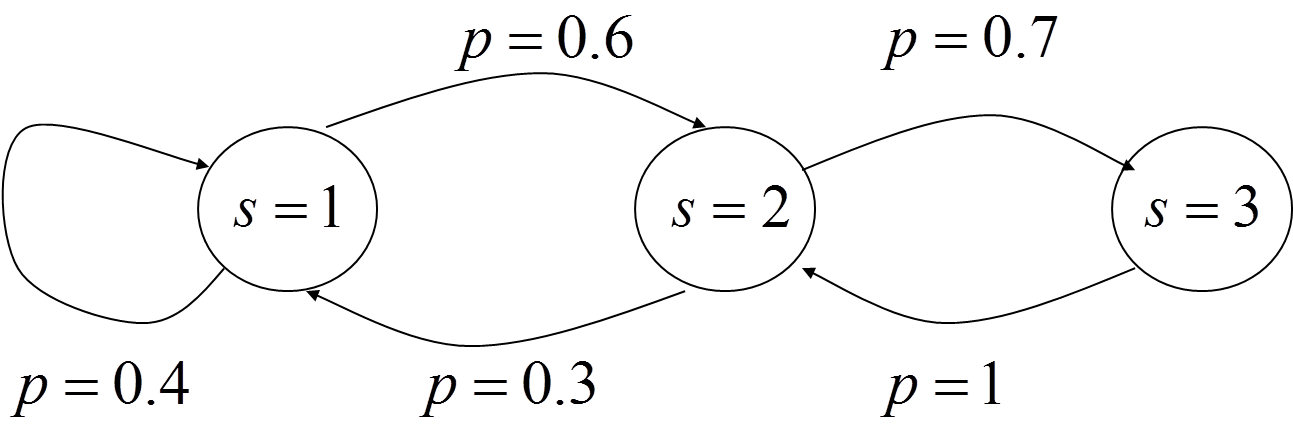
\includegraphics[width=0.7\textwidth]{figures/lecture4_a}\\
  \caption{Markov chain}\label{fig:MC}
  \end{centering}
\end{figure}

A graphical description of a controlled Markov chain is a bit more
complicated because of the additional action variable. We obtain the
diagram (drawn for state $\state = 1$ only, and for a given time
$\ttime$) in Figure \ref{fig:MDP}, reflecting the following
transition probabilities:
\[\begin{array}{l}
p(\state' = 2|\state = 1,\action = 1) = 1\\
p(\state'|\state = 1,\action = 2) = \left\{ {\begin{array}{*{20}{c}}
{0.3}&:&{\state' = 1}\\
{0.2}&:&{\state' = 2}\\
{0.5}&:&{\state' = 3}
\end{array}} \right.
\end{array}\]

\begin{figure}
  % Requires \usepackage{graphicx}
  \begin{centering}
  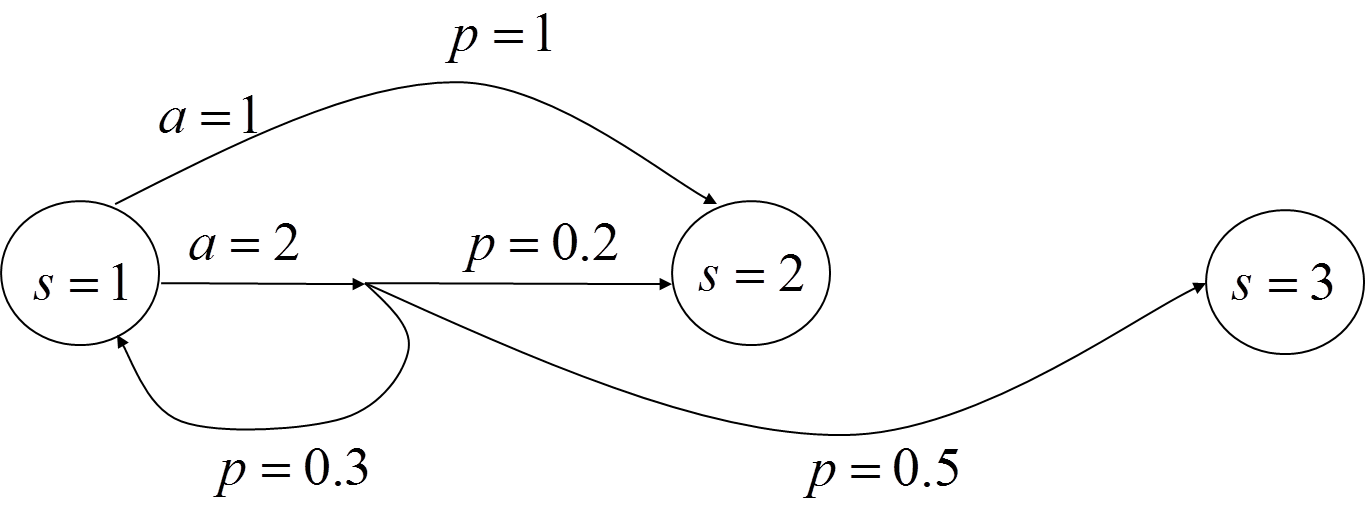
\includegraphics[width=0.7\textwidth]{figures/lecture4_b}\\
  \caption{Controlled Markov chain}\label{fig:MDP}
  \end{centering}
\end{figure}


\paragraph{State-equation notation:}
The stochastic state dynamics can be equivalently defined in terms of a state equation of the form
                                                   \[{\state_{\ttime + 1}} = {f_\ttime}({\state_\ttime},{\action_\ttime},{w_\ttime}),\]
where ${w_\ttime}$ is a random variable (RV).
    If  ${({w_\ttime})_{\ttime \ge 0}}$ is a sequence of independent RVs, and further each ${w_\ttime}$ is independent of the ``past"  $({\state_{\ttime - 1}},{\action_{\ttime - 1}}, \ldots {\state_0})$, then ${({\state_\ttime},{\action_\ttime})_{\ttime \ge 0}}$ is a controlled Markov process.
    For example, the state transition law of the last example can be written in this way, using
                  ${w_\ttime} \in \{ 4,5,6\} $,  with  ${p_w}(4) = 0.3,\;{p_w}(5) = 0.2,\;{p_w}(6) = 0.5$
and, for ${\state_\ttime} = 1$:
    \[\begin{array}{l}
    {f_\ttime}(1,1,{w_\ttime}) = 2\\
    {f_\ttime}(1,2,{w_\ttime}) = {w_\ttime} - 3
    \end{array}\]
  This state algebraic equation notation is especially useful for problems with continuous state space, but also for some models with discrete states.
Equivalently, we can write
    \[
 {f_\ttime}(1,2,{w_\ttime}) = 1\cdot \I[{w_\ttime}=4]+2\cdot \I[{w_\ttime}=5]+3\cdot \I[{w_\ttime}=6] ,
    \]
where $\I[\cdot]$ is the indicator function.

Next we recall the definitions of control policies from Chapter \ref{chapter:DDP}.

\paragraph{Control Policies}
\begin{itemize}
  \item
A general or \textbf{history-dependent deterministic} control policy
$\policy  = {({\policy _\ttime})_{\ttime \in {\mathbb{T}}}}$ is a
mapping from each possible history ${\history_\ttime} =
({\state_0},{\action_0}, \ldots ,{\state_{\ttime -
1}},{\action_{\ttime - 1}},{\state_\ttime})$, and time $\ttime \in
\T$, to an action ${\action_\ttime} = {\policy
_\ttime}({\history_\ttime}) \in {\Actions_\ttime}$.  We denote the
set of general policies by ${\Pi _{HD}}$.
  \item
A \textbf{Markov deterministic} control policy $\policy $ is allowed
to depend on the current state and time only, i.e., ${\action_\ttime} =
{\policy _\ttime}({\state_\ttime})$.   We denote the set of Markov
deterministic policies by ${\Pi _{MD}}$.
  \item
For stationary models, we may define \textbf{stationary
deterministic} control policies that depend on the current state
alone. A stationary policy is defined by a single mapping $\policy
:\States \to \Actions$, so that  ${\action_\ttime} = \policy
({\state_\ttime})$ for all $\ttime \in {\T}$. We denote the set of
stationary policies by ${\Pi _{SD}}$.
  \item Evidently, ${\Pi_{HD}} \supset {\Pi_{MD}} \supset {\Pi_{SD}}$.
\end{itemize}

\paragraph{Randomized Control policies}
\begin{itemize}
  \item The control policies defined above specify deterministically the action to be taken at each stage. In some cases we want to allow for a random choice of action.
  \item A general randomized control policy assigns to each possible history ${\history_\ttime}$ a probability distribution ${\policy _\ttime}( \cdot |{\history_\ttime})$ over the action set ${\Actions_\ttime}$.
  That is,  $\Pr( {\action_\ttime} = \action|{\history_\ttime})  = {\policy _\ttime}(\action|{\history_\ttime})$. We denote the set of history-dependent stochastic policies by ${\Pi _{HS}}$.
  \item Similarly, we can define the set ${\Pi _{MS}}$ of Markov stochastic control policies, where ${\policy _\ttime}( \cdot |{\history_\ttime})$ is replaced by ${\policy _\ttime}( \cdot |{\state_\ttime})$, and the set ${\Pi _{SS}}$ of stationary stochastic control policies, where ${\policy _\ttime}( \cdot |{\state_\ttime})$ is replaced by  $\policy ( \cdot
  |{\state_\ttime})$, namely the policy is independent of the time.
  \item Note that the set ${\Pi _{HS}}$ includes all other policy sets as special cases.
\end{itemize}

\paragraph{The Induced Stochastic Process}
Let  ${p_0} = \{ {p_0}(\state),\state \in {\States_0}\} $ be a
probability distribution for the initial state ${\state_0}$. (Many
times we will assume that the initial state is deterministic and
given by $\state_0$.) A control policy $\policy \in {\Pi _{HS}}$,
together with the transition law $P = \{
{p_\ttime}(\state'|\state,\action)\} $ and the initial state
distribution ${p_0} = ({p_0}(\state),\;\state \in {\States_0})$,
induces a probability distribution over any finite state-action
sequence ${\history_\tHorizon} = ({\state_0},{\action_0}, \ldots
,{\state_{\tHorizon - 1}},{\action_{\tHorizon -
1}},{\state_\tHorizon})$, given by
\[\Pr({\history_\tHorizon}) = {p_0}({\state_0})\prod\limits_{\ttime = 0}^{\tHorizon -1} {p_\ttime({\state_{\ttime + 1}}|{\state_\ttime},{\action_\ttime}){\policy _\ttime}({\action_\ttime}|{\history_\ttime})} ,\]
where ${\history_\ttime} = ({\state_0},{\action_0}, \ldots
,{\state_{\tHorizon -1}},{\action_{\tHorizon -1}},{\state_\ttime})$.
%
To see this, observe the recursive relation:
%\[
\begin{align*}
\Pr({\history_{\ttime + 1}}) &= \Pr({\history_\ttime},{\action_\ttime},{\state_{\ttime + 1}}) = \Pr({\state_{\ttime + 1}}|{\history_\ttime},{\action_\ttime})\Pr({\action_\ttime}|{\history_\ttime})\Pr({\history_\ttime})\\
 &= {p_\ttime}({\state_{\ttime + 1}}|{\state_\ttime},{\action_\ttime}){\policy _\ttime}({\action_\ttime}|{\history_\ttime})\Pr({\history_\ttime}).
\end{align*}
%\]
In the last step we used the conditional Markov property of the
controlled chain: $\Pr({\state_{\ttime +
1}}|{\history_\ttime},{\action_\ttime}) = {p_\ttime}({\state_{\ttime
+ 1}}|{\state_\ttime},{\action_\ttime})$, and the definition of the
control policy $\policy_\ttime $. The required formula follows by
recursion.

Therefore, the state-action sequence ${\history_\infty } =
{({\state_k},{\action_k})_{k \ge 0}}$ can now be considered a
stochastic process. We denote the probability law of this stochastic
process by ${\Pr^{\policy ,{p_0}}}( \cdot )$. The corresponding
expectation operator is denoted by ${\E^{\policy ,{p_0}}}( \cdot )$.
When the initial state ${\state_0}$ is deterministic (i.e.,
${p_0}(\state)$ is concentrated on a single state $\state$), we may
simply write ${\Pr^{\policy ,s}}( \cdot )$  or ${\Pr^\policy }( \cdot
|{\state_0} = \state)$.

Under a Markov control policy, the state sequence
${({\state_\ttime})_{\ttime \ge 0}}$ becomes a \emph{Markov chain},
with transition probabilities:
\[\Pr({\state_{\ttime + 1}} = \state'|{\state_\ttime} = \state) = \sum\nolimits_{\action \in {\Actions_\ttime}} {{p_\ttime}} (\state'|\state,\action){\policy _\ttime}(\action|\state).\]
This follows since:
\begin{align*}
\Pr({\state_{\ttime + 1}} = \state'|{\state_\ttime} = \state) & =
\sum\nolimits_{\action \in {\Actions_\ttime}} \Pr({\state_{\ttime +
1}} = \state', \action|{\state_\ttime} = \state)  \\
& =\sum\nolimits_{\action \in {\Actions_\ttime}} \Pr({\state_{\ttime
+ 1}} = \state'|{\state_\ttime} = \state,\action) \Pr(\action |
\state_\ttime=\state) \\
&= \sum\nolimits_{\action \in {\Actions_\ttime}} {{p_\ttime}}
(\state'|\state,\action){\policy _\ttime}(\action|\state)
\end{align*}
 \ymignore{
\begin{exercise}{Prove this!}\end{exercise}
}

%\begin{proof} add \end{proof}

If the controlled Markov chain is stationary (time-invariant) and the control policy is stationary, then the induced Markov chain is stationary as well.



\begin{remark}
For most non-learning optimization problems, Markov policies suffice to achieve the optimum.
\end{remark}
\begin{remark}
Implicit in these definitions of control policies is the assumption
that the current state ${\state_\ttime}$ can be fully observed
before the action ${\action_\ttime}$ is chosen . If this is not the
case we need to consider the problem of a Partially Observed MDP
(POMDP), which is more involved and will be discussed in Chapter \ref{chapter:POMDP}.
\end{remark}

\section{Performance Criteria}

\subsection{Finite Horizon Return}
Consider the finite-horizon return, with a fixed time horizon
$\tHorizon$. As in the deterministic case, we are given a running
reward function ${\reward_\ttime} = \{
{\reward_\ttime}(\state,\action):\state \in {\States_\ttime},\action
\in {\Actions_\ttime}\} $ for $0 \le \ttime \le \tHorizon -1$, and a
terminal reward function ${\reward_\tHorizon} = \{
{\reward_\tHorizon}(\state):\state \in {\States_\tHorizon}\} $.  The
obtained reward is  $R_\ttime =
{\reward_\ttime}({\state_\ttime},{\action_\ttime})$ at times $\ttime
\le \tHorizon -1$, and ${R_\tHorizon} =
{\reward_\tHorizon}({\state_\tHorizon})$ at the last stage. (Note
that $\state_\ttime,\action_\ttime$ and $\state_\tHorizon$ are
random variables that depend both on the policy $\policy$ and the
stochastic transitions.)
 Our
general goal is to maximize the cumulative return:
\[
\sum\limits_{\ttime = 0}^\tHorizon {{R_\ttime}}  = \sum\limits_{\ttime = 0}^{\tHorizon -1}
{{\reward_\ttime}({\state_\ttime},{\action_\ttime}) +
{\reward_\tHorizon}({\state_\tHorizon})} .
\]
However, since the system is
stochastic, the cumulative return will generally be a random variable, and we
need to specify in which sense to maximize it. A natural first
option is to consider the expected value of the return. That is,
define:
\[\Value_\tHorizon^\policy (\state) = {\E^\policy }(\sum\limits_{\ttime = 0}^\tHorizon {{R_\ttime}} |{\state_0} = \state) \equiv {\E^{\policy ,s}}(\sum\limits_{\ttime = 0}^\tHorizon {{R_\ttime}} ) .\]
Here $\policy $ is the control policy as defined above, and $\state$
denotes the initial state. Hence,  $\Value_\tHorizon^\policy
(\state)$ is the expected cumulative return under the control policy
$\policy $.  Our goal is to find an optimal control policy that
maximizes $\Value_\tHorizon^\policy
 (\state)$.

\paragraph{Remarks:}
\begin{enumerate}
  \item Reward dependence on the next state:  In some problems, the obtained reward may depend on the next state as well: ${R_\ttime} = {\tilde \reward_\ttime}({\state_\ttime},{\action_\ttime},{\state_{\ttime + 1}})$.  For control purposes, when we only consider the expected value of the reward, we can reduce this reward function to the usual one by defining
\[{\reward_\ttime}(\state,\action) \buildrel \Delta \over = \E({R_\ttime}|{\state_\ttime} = \state,{\action_\ttime} = \action) \equiv \sum\nolimits_{\state' \in S} {p(\state'|\state,\action){{\tilde r}_\ttime}(} s,a,\state')\]
  \item Random rewards:  The reward ${R_\ttime}$ may also be random, namely a random variable whose distribution depends on $({\state_\ttime},{\action_\ttime})$.  This can also be reduced to our standard model for planning purposes by looking at the expected value of ${R_\ttime}$, namely \[{\reward_\ttime}(\state,\action) = \E({R_\ttime}|{\state_\ttime} = \state,{\action_\ttime} =
  \action).\]
  \item Risk-sensitive criteria: The expected cumulative return is by far the most common goal for planning. However, it is not the only one possible. For example, one may consider the following risk-sensitive  return function:
\[\Value_{{\tHorizon,\lambda }}^\policy (\state) = \frac{1}{\lambda }\log {\E^{\policy ,s}}(\exp (\lambda \sum\limits_{\ttime = 0}^\tHorizon {{R_\ttime}} )).\]
For $\lambda  > 0$, the exponent gives higher weight to high rewards, and the opposite for $\lambda  < 0$.
\end{enumerate}

In the case that the rewards are stochastic, but have a discrete
support, we can construct an equivalent MDP in which all the rewards
are deterministic and has the same distribution of rewards. This
implies that the important challenge is the stochastic state
transition function, and the rewards can be assumed to be
deterministic.
%
Formally, given a trajectory we define a {\em rewards trajectory} as
the sub-trajectory that includes only the rewards, i.e., for a trajectory $(\state_0,\action_0,reward_0,state_1, \ldots)$ the reward trajectory is  $(\reward_0, \reward_1, \ldots)$.


%[Add HW to do the same for discounted]

\begin{theorem}
\label{thm:K-rewards}
%
 Given an MDP $M(\States,\Actions,p,\reward,\state_0)$,
where the rewards are stochastic, with support ${\cal
K}=\{1,\ldots,k\}$, there is an MDP $M'(\States\times {\cal
K},\Actions,p',\reward',\state_0')$, and a mapping of
policies $\policy$ of $M$ to $\policy'$ policies of $M'$, such that:
running $\pi$ in $M$ for horizon $\tHorizon$ generates reward
trajectory $R=(R_0, \ldots , R_{\tHorizon})$ and running $\pi'$ in
$M'$ for horizon $\tHorizon+1$ generates reward trajectory $R=(R_1,
\ldots , R_{\tHorizon+1})$, then the distribution of $R$ and $R'$
are identical.
%$\Value_\tHorizon^{\policy,M}(\state_0)=\Value_{\tHorizon+1}^{\policy_1,M_1}$
\end{theorem}

\begin{proof}
The basic idea is to encode the rewards in the states of $M'$ which
are
%. Let ${\cal K}=\{1,\ldots , k\}$. We define a new state space
$\States\times {\cal K}=\States'$.
%
For each $(\state,i)\in \States'$ and action $\action\in\Actions$ we
have
$p'_t((\state',j)|(\state,i),\action)=p_t(\state'|\state,\action)\Pr[R_t(\state,\action)=j]$,
and
$p'_{\tHorizon}((\state',j)|(\state,i))=\I(\state'=\state)\Pr[R_{\tHorizon}(\state)=j]$.
The reward is $\reward'_t((\state,i),\action)=i$. The initial state
is $\state'_0=(\state_0,0)$.

For any policy $\policy(\action|\state)$ in $M$ we have a policy
$\policy'$ is $M'$ where
$\policy'(\action|(\state,i))=\policy(\action|\state)$.

We map trajectories of $M$ to trajectories of $M'$ which have
identical probabilities. A trajectory $(\state_0, \action_0 , R_0 ,$
$\state_1,\action_1,R_1, \state_2 \ldots, R_{\tHorizon})$ is map to
$((\state_0,0), \action_0 , 0 ,$ $ (\state_1,R_0),\action_1,R_0,
(\state_2,R_1) \ldots, R_{\tHorizon+1})$. Let $R$ and $R'$ be the
respective reward trajectories.
%
Clearly, the two trajectories have identical probabilities. This
implies that the rewards trajectories $R$ and $R'$ have are
identical probabilities (up to a shift of one in the index).
% Therefore the policies have identical return.l
\end{proof}

Theorem~\ref{thm:K-rewards} requires the number of rewards be
bounded, and guarantees that the reward distribution be identical.
In the case that the rewards are continuous, we can have a similar
guarantee for linear return functions.


\begin{theorem}
Given an MDP $M(\States,\Actions,p,\reward,\state_0)$, where the
rewards are stochastic, with support $[0,1]$, there is an MDP
$M'(\States,\Actions,p,\reward',\state_0)$, where the rewards are
stochastic, with support $\{0,1\}$,
% and a mapping of policies
%$\policy\in \Pi_{MS}$ of $M$ to $\policy'$ policies of $M'$,
such that for any policy $\policy\in \Pi_{MS}$ the distribution of
the expected rewards trajectory is identical.
%$\Value_\tHorizon^{\policy,M}(\state_0)=\Value_{\tHorizon+1}^{\policy',M'}(\state'_0)$
\end{theorem}

\begin{proof}
We simply change the reward of $(\state,\action)$ to be $\{0,1\}$ by
changing them to be a Bernoulli random variables with a parameter
$\reward_t(\state,\action)$, i.e.,
$\Pr[\Rewards_\ttime(\state,\action)=1]=\reward_\ttime(\state,\action)$
and
$\Pr[\Rewards_\ttime(\state,\action)=0]=1-\reward_\ttime(\state,\action)$.
Clearly, the expected value of the rewards is identical. Further,
since $\policy\in \Pi_{MS}$, it depends only of $\state$ and
$\ttime$, which implies that the behavior (states and actions) will
be identical in $M$ and $M'$.
\end{proof}

We have also established the following corollary.

\begin{corollary}
Given an MDP $M(\States,\Actions,p,\reward,\state_0)$, where the
rewards are stochastic, with support $[0,1]$, there is an MDP
$M'(\States\times \{ 0,1\},\Actions,p',\reward',\state'_0)$, and a
mapping of policies $\policy\in \Pi_{MS}$ of $M$ to $\policy'\in
\Pi_{MD}$ policies of $M'$, such that
%the distribution rewards trajectory  is identical.
$\Value_\tHorizon^{\policy,M}(\state_0)=\Value_{\tHorizon+1}^{\policy',M'}(\state'_0)$
\end{corollary}

%\begin{proof}
%Similar to before, we encode the rewards in the states of $M'$ which
%are
%%. Let ${\cal K}=\{1,\ldots , k\}$. We define a new state space
%$\States\times \{0,1\}=\States'$.
%%
%For each $(\state,i)\in \States'$ and action $\action\in\Actions$ we
%have
%$p'((\state',1)|(\state,b),\action)=p(\state'|\state,\action)\reward(\state,\action)$,
%and
%$p'((\state',0)|(\state,b),\action)=p(\state'|\state,\action)(1-\reward(\state,\action))$,
%The reward is $\reward'((\state,b),\action)=b$ for $b\in\{0,1\}$.
%The initial state is $\state'_0=(\state_0,0)$.
%
%For any policy $\policy(\action|\state)$ in $M$ we have a policy
%$\policy'$ is $M'$ define as follows:
%$\policy'(\action|(\state,b))=\policy(\action|\state)$.
%
%As before, we can map trajectories of $M$ to trajectories in $M'$ by
%simply having $\state_0, \action_0 , R_0 , \state_1,\action_1,R_1,
%\state_2 \ldots$ to $(\state_0,0), \action_0 , 0 ,
%(\state_1,b_0),\action_1,b_0, (\state_2,b_1) \ldots$ . Since
%$\E[R_t]=\E[b_{t+1}]$, the expected returns are identical.
%\end{proof}



\subsection{Infinite Horizon Problems}
We next consider planning problems that extend to an infinite time
horizon, $\ttime = 0,1,2, \ldots $. Such planning problems arise
when the system in question is expected to operate for a long time,
or a large number of steps, possibly with no specific ``closing"
time. Infinite horizon problems are most often defined for
stationary problems. In that case, they enjoy the important
advantage that optimal policies can be found among the class of
stationary policies.  We will restrict attention here to stationary
models. As before, we have the running reward function
$\reward(\state,\action)$, which extends to all $\ttime\ge 0$. The
expected reward obtained at stage $\ttime$ is $\E[{R_\ttime}] =
\reward({\state_\ttime},{\action_\ttime})$.

\paragraph{Discounted return:} The most common performance criterion for infinite horizon problems is the expected discounted return:
\[\Value_\discount ^\policy (\state) = {\E^\policy }(\sum\limits_{\ttime = 0}^\infty  {{\discount ^t}\reward({\state_\ttime},{\action_\ttime})} |{\state_0} = \state) \equiv {\E^{\policy ,s}}(\sum\limits_{\ttime = 0}^\infty  {{\discount ^t}\reward({\state_\ttime},{\action_\ttime})} )\;,\]
where $0 < \discount  < 1$ is the discount factor. Mathematically,
the discount factor ensures convergence of the sum (whenever the
reward sequence is bounded). This makes the problem ``well behaved",
and relatively easy to analyze. The discounted return is discussed
in Chapter \ref{chapter:disc}.

\paragraph{Average return:}  Here we are interested to maximize the long-term average return. The most common definition of the long-term average return is
\[\Value_{av}^\policy (\state) = \mathop {\lim \inf }\limits_{\tHorizon \to \infty } {\E^{\policy ,s}}(\frac{1}{\tHorizon}\sum\limits_{\ttime = 0}^{\tHorizon -1} {\reward({\state_\ttime},{\action_\ttime})} )\]
The theory of average-return planning problems is more involved, and
relies to a larger extent on the theory of Markov chains (see
Chapter~\ref{chapter:MC}). The average return is discussed in
Chapter \ref{chapter:average}.



\subsection{Stochastic Shortest-Path Problems}
In an important class of planning problems, the time horizon is not
set beforehand, but rather the problem continues until a certain
event occurs. This event can be defined as reaching some goal state.
Let  ${\States_G} \subset \States$ define the set of \emph{goal
states}. Define
\[\tau  = \inf \{ \ttime \ge 0:{\state_\ttime} \in {\States_G}\} \]
as the first time in which a goal state is reached. The total expected return for this problem is defined as:
\[\Value_{ssp}^\policy (\state) = {\E^{\policy ,\state}}(\sum\limits_{\ttime = 0}^{\tau  - 1} {\reward({\state_\ttime},{\action_\ttime})}  + {\reward_G}({\state_\tau }))\]
Here ${\reward_G}(\state),\;\state \in {\States_G}$ specified the
reward at goal states. Note that the length of the run $\tau$ is a random variable.



Stochastic shortest path includes, naturally, the finite horizon case. This can be shown by creating a leveled MDP where at each time step we move to the next level and terminate at level $\tHorizon$.
Specifically, we define a new state space $\States'=\States\times \T$, transition function $p((\state',i+1)|\state,\action)=p(\state'|\state,\action)$, and goal states $\States_G=\{(\state,\tHorizon):\state \in\States\}$.

Stochastic shortest path includes also the discounted infinite
horizon. To see that, add a new goal state, and from each state with
probability $1-\discount$ jump to the goal state and terminate. The
expected return of a policy would be the same in both models.
Specifically, we add a state $\state_G$, such that
$p(\state_G|\state,\action)=1-\discount$, for any state
$\state\in\States$ and action $\action\in\Actions$ and
$p(\state'|\state,\action)=\discount p(\state'|\state,\action)$. The
probability that we do not terminate by time $\ttime$ is exactly
$\discount^\ttime$. Therefore, the expected return is
$\sum_{t=1}^\infty \discount^t\reward(\state_t,\action_t)$ which is
identical to the discounted return.

This class of problems provides a natural extension of the standard
shortest-path problem to stochastic settings.  Some conditions on
the system dynamics and reward function must be imposed for the
problem to be well posed (e.g., that a goal state may be reached
with probability one). Such problems are known as stochastic
shortest path problems, or also episodic MDP planning problems. See
more in Chapter \ref{chapter:ssp}.

\section{Sufficiency of Markov Policies}
In all the performance criteria defined above, the criterion is
composed of sums of terms of the form
$\E({\reward_\ttime}({\state_\ttime},{\action_\ttime}))$. It follows
that if two control policies induce the same marginal probability
distributions ${q_\ttime}({\state_\ttime},{\action_\ttime})$ over
the state-action pairs $({\state_\ttime},{\action_\ttime})$ for all
$\ttime \ge 0$, they will have the same performance for any linear
return function.

Using this observation, the next claim implies that it is enough to
consider the set of (stochastic) Markov policies in the above
planning problems.

\begin{proposition}\label{prop:sufficient} Let  $\policy  \in {\Pi _{HS}}$ be a general (history-dependent, stochastic) control policy.  Let
\[p_\ttime^{\policy ,{\state_0}}(\state,\action) = {P^{\policy ,{\state_0}}}({\state_\ttime} = \state,{\action_\ttime} = \action),\quad \;\;(\state,\action) \in {\States_\ttime} \times {\Actions_\ttime}\]
Denote the marginal distributions induced by
$q_t({\state_\ttime},{\action_\ttime})$ on the state-action pairs
$({\state_\ttime},{\action_\ttime})$, for all $\ttime \ge 0$. Then there
exists a stochastic Markov policy $\tilde \policy \in {\Pi_{MS}}$
that induces the same marginal probabilities (for all initial states
${\state_0}$).
\end{proposition}

\ymignore{
\begin{exercise}[\textbf{Challenge Problem 1}] Prove Proposition \ref{prop:sufficient}.
Note: If you consult a reference or a friend, mention that in your solution.
\end{exercise}
}

In Chapter~\ref{chapter:DDP}  we showed for Deterministic Decision
Process for the finite horizon that there is an optimal
deterministic policy. The proof that every stochastic history
dependent strategy has an equivalent stochastic Markovian policy
(Theorem~\ref{chp2:HS-MS}) showed how to generate the same
state-action distribution, and applies to other setting as well. The
proof that every stochastic Markovian policy has a deterministic
Markovian policy (Theorem~\ref{chp2:stochastic-deterministic})
depended on the finite horizon, but it is easy to extend it to any
linear return function as well.

\section{Finite-Horizon Dynamic Programming}

Recall that we consider the expected total reward criterion, which we denote as
\[{\Value^\policy }({\state_0}) = {\E^{\policy ,{\state_0}}}\left( {\sum\nolimits_{\ttime = 0}^{\tHorizon -1} {{\reward_\ttime}({\state_\ttime},{\action_\ttime}) + {\reward_\tHorizon}({\state_\tHorizon})} } \right)\;,\]
where $\policy $ is the control policy used, and ${\state_0}$ is a
given initial state. We wish to maximize the expected return
${\Value^\policy }({\state_0})$ over all control policies, and find
an optimal policy ${\policy ^*}$ that achieves the maximal expected
return ${\Value^*}({\state_0})$ for all initial states ${\state_0}$.
Thus,
\[{\Value^*_\tHorizon}({\state_0}) \buildrel \Delta \over = {\Value^{\policy *}_\tHorizon}({\state_0}) = \mathop {\max }\limits_{\policy  \in {\Pi _{HS}}} {\Value^\policy_\tHorizon }({\state_0})\]


\subsection{The Principle of Optimality}
The celebrated principle of optimality (stated by Bellman) applies
to a large class of multi-stage optimization problems, and is at the
heart of Dynamic Programming. As a general principle, it states
that:
\begin{center}
\textbf{The tail of an optimal policy is optimal for the ``tail"
problem.}
\end{center}

This principle is not an actual claim, but rather a guiding
principle that can be applied in different ways to each problem. For
example, considering our finite-horizon problem, let ${\policy ^*} =
({\policy _0}, \ldots ,{\policy _{\tHorizon -1}})$ denote an optimal
Markov policy. Take any state ${\state_\ttime} = \state'$ which has
a positive probability to be reached under ${\policy ^*}$, namely
${P^{\policy^* ,{\state_0}}}({\state_\ttime} = \state')
> 0$. Then the tail policy $\policy^*_{\ttime:\tHorizon}=({\policy _\ttime}, \ldots ,{\policy _{\tHorizon -1}})$ is optimal for the ``tail" criterion $\Value_{\ttime:\tHorizon}^\policy
(\state') = {\E^\policy }\left( {\sum\nolimits_{k = t}^\tHorizon
{{R_k}|{\state_\ttime} = \state'} } \right)$.

Note that the reverse is not true. The prefix of the optimal policy
is not optimal for the ``prefix'' problem. When we plan for a long
horizon, we might start with non-greedy actions, so we can improve
our return in later time steps. Specifically, the first action taken
does not have to be the optimal action for horizon $\tHorizon=1$,
for which the greedy action is optimal.


\subsection{Dynamic Programming for Policy Evaluation}\label{sss:pol_eval}
As a ``warmup", let us evaluate the reward of a given policy. Let
$\policy  = ({\policy _0}, \ldots ,{\policy _{\tHorizon -1}})$ be a
given Markov policy. Define the following reward-to-go function, or
value function:
\[V_k^\policy (\state) = {\E^\policy }\left( {\sum\nolimits_{\ttime = k}^\tHorizon {{R_\ttime}|{\state_k} = \state} } \right)\]
Observe that $V_0^\policy ({\state_0}) = {\Value^\policy }({\state_0})$.

\begin{lemma}[\textbf{Value Iteration}]\label{lem:finite_horizon_VI} $V_k^\policy (\state)$ may be computed by the backward recursion:
\[V_k^\policy (\state) = {\left\{ {{\reward_k}(\state,\action) + \sum\nolimits_{\state' \in {\States_{k + 1}}} {{p_k}(\state'|\state,\action)} \;V_{k + 1}^\policy (\state')} \right\}_{a = {\policy _k}(\state)}}\;,\quad \forall \state \in {\States_k}\]
for $k = \tHorizon -1, \ldots ,0$,  starting with
$V_\tHorizon^\policy (\state) = {\reward_\tHorizon}(\state)$.
\end{lemma}
\begin{proof}
Observe that:
\begin{align*}
V_k^\policy (\state) &= {\E^\policy }\left( {{R_k} + \sum\nolimits_{\ttime = k + 1}^\tHorizon {{R_\ttime}|} \;{\state_k} = \state,{\action_k} = {\policy _k}(\state)} \right)\\
 &= {\E^\policy }\left( {{\E^\policy }\left( {{R_k} + \sum\nolimits_{\ttime = k + 1}^\tHorizon {{R_\ttime}} |\;{\state_k} = \state,{\action_k} = {\policy _k}(\state),{\state_{k + 1}}} \right)|{\state_k} = \state,{\action_k} = {\policy _k}(\state)} \right)\\
 &= {\E^\policy }\left( {\reward_kß({\state_k},{\action_k}) + V_{k + 1}^\policy ({\state_{k + 1}})|{\state_k} = \state,{\action_k} = {\policy _k}(\state)} \right)\\
 &= {\reward_k}(s,{\policy _k}(\state)) + \sum\nolimits_{\state' \in {\States_{k + 1}}} {{p_k}(\state'|s,{\policy _k}(\state))} \;V_{k + 1}^\policy (\state')
\end{align*}
The first identity is simply writing the value function explicitly,
starting at state $\state$ at time $k$ and using action
$\action=\policy_k(\state)$.  We split the sum to $R_k$, immediate
reward, and the sum of other rewards.
%, which will be convenient later.
The second identity uses the law of total probability, we are
conditioning on state $\state_{k+1}$, and taking the expectation
over it.
%
The third identity observes that the expected value of the sum is actually the value function at $\state_{k+1}$. The last identity writes the expectation over $\state_{k+1}$ explicitly.
\end{proof}

\paragraph{Remarks:}
\begin{itemize}
  \item Note that $\sum\nolimits_{\state' \in {\States_{k + 1}}} {{p_k}(\state'|\state,\action)} \;V_{k + 1}^\policy (\state') = {\E^\policy }(V_{k + 1}^\policy ({\state_{k + 1}})|{\state_k} = \state,{\action_k} = \action)$.
  \item For the more general reward function ${\tilde \reward_\ttime}(\state,\action,\state')$, the recursion takes the form
                     \[V_k^\policy (\state) = {\left\{ {\sum\nolimits_{\state' \in {\States_{k + 1}}} {{p_k}(\state'|\state,\action)} [{\tilde \reward_k}(\state,\action,\state') + V_{k + 1}^\policy (\state')]} \right\}_{\action = {\policy _k}(\state)}}\;.\]
                      A similar observation applies to the Dynamic Programming
equations in the next section.
\end{itemize}

\subsection{Dynamic Programming for Policy Optimization}

We next define the optimal value function at each time $k \ge 0$ :
\[
V_k^{*}(\state) = \mathop {\max }\limits_{{\policy ^k}}
{\E^{{\policy ^k}}}\left( {\sum\nolimits_{\ttime = k}^\tHorizon
{{R_\ttime}|{\state_k} = \state} } \right),\quad \,\state \in
{\States_k} \;,
\]
where the maximum is taken over ``tail" policies ${\policy ^k} =
({\policy_k}, \ldots ,{\policy _{\tHorizon -1}})$ that start from
time $k$. Note that ${\policy ^k}$ is allowed to be a general
policy, i.e., history-dependent and stochastic. Obviously,
${V_0}({\state_0}) = {\Value^*}({\state_0})$.

\begin{theorem}[\textbf{Finite-horizon Dynamic Programming}]\label{thm:finite_horizon_DP}
The following holds:
\begin{enumerate}
\item
Backward recursion:  Set $V_\tHorizon^{}(\state) = {\reward_\tHorizon}(\state)$ for $\state\in {\States_\tHorizon}$.\\
     For $k = \tHorizon -1, \ldots ,0$, $V_k^{}(\state)$  compute using the following recursion:
\[V_k^{}(\state) = \mathop {\max }\limits_{\action \in {\Actions_k}} \left\{ {{\reward_k}(\state,\action) + \sum\nolimits_{\state' \in {\States_{k + 1}}} {{p_k}(\state'|\state,\action)\,} V_{k + 1}^{}(\state')} \right\},  \quad  \state \in {\States_k}.\]
We have that $V_k(s)=V^*_k(s)$.
\item
Optimal policy: Any Markov policy ${\policy ^*}$ that satisfies, for $\ttime = 0, \ldots ,\tHorizon -1$,
\[\policy _\ttime^*(\state) \in \mathop {\arg \max }\limits_{\action \in {\Actions_\ttime}} \left\{ {{\reward_\ttime}(\state,\action) + \sum\nolimits_{\state' \in {\States_{\ttime + 1}}} {{p_\ttime}(\state'|\state,\action)\,} V_{\ttime + 1}^{}(\state')} \right\},\quad \forall \state \in {\States_\ttime},\]
is an optimal control policy. Furthermore, ${\policy ^*}$ maximizes
${\Value^\policy }({\state_0})$ simultaneously for every initial state
${\state_0} \in {\States_0}.$
\end{enumerate}
\end{theorem}
Note that Theorem \ref{thm:finite_horizon_DP} specifies an optimal control policy which is a deterministic Markov policy.

\begin{proof}
\textbf{Part (i):}

We use induction to show that the stated backward recursion indeed
yields the optimal value function $V_\ttime^*$. The idea is simple,
but some care is needed with the notation since we consider general
policies, and not just Markov policies.

For the base of the induction we start with $\ttime=\tHorizon$. The
equality $V_\tHorizon^{}(\state) = {\reward_\tHorizon}(\state)$
follows directly from the definition of $V_\tHorizon^{}$. Clearly
this is also the optimal value function $V^*_{\tHorizon}$.

We proceed by backward induction. Suppose that $V_{k +
1}^{}(\state)$ is the optimal value function for time $k + 1$, i.e.,
$V_{k + 1}^{}(\state)=V^*_{k+1}$ . We need to show that
$V_k^{}(\state) = V^*_k(\state)$ and we do it by showing that
$V^*_k(\state)={W_k}(\state)$, where
 \[{W_k}(\state) \buildrel \Delta \over = {\max _{\action \in {\Actions_k}}}\left\{ {{\reward_k}(\state,\action) + \sum\nolimits_{\state' \in {\States_{k + 1}}} {{p_k}(\state'|\state,\action)\,} V_{k + 1}^{}(\state')} \right\}.\]
We will first establish that $V_k^{*}(\state) \ge {W_k}(\state)$,
and then that $V_k^{*}(\state) \le {W_k}(\state)$.

(a) We first show that $V_k^{*}(\state) \ge {W_k}(\state)$. For that
purpose, it is enough to find a policy ${\policy ^k}$ so that
$V_k^{{\policy ^k}}(\state) = {W_k}(\state)$, since $V^*_k(s)\geq
V^\pi_k(s)$ for any strategy $\pi$.

Fix $\state \in {\States_k}$, and define ${\policy ^k}$ as follows:
Choose ${\action_k} = \bar \action$, where
\[\bar{\action} \in \mathop {\arg \max }\limits_{\action \in {\Actions_k}} \left\{ {{\reward_k}(\state,\action) + \sum\nolimits_{\state' \in {\States_{k + 1}}} {{p_k}(\state'|\state,\action)} \,V_{k + 1}^{}(\state')} \right\},\]
and then, after observing  ${\state_{k + 1}} = \state'$, proceed
with the optimal tail policy ${\policy ^{k + 1}}(\state')$ that
obtains $V_{k + 1}^{{\policy ^{k + 1}}(\state')}(\state') = {V_{k +
1}}(\state')$. Proceeding similarly to
%Subsection \ref{sss:pol_eval} above
the proof of Lemma~\ref{lem:finite_horizon_VI} (value iteration for
a fixed policy), we obtain:
\begin{align}
V_k^{{\policy ^k}}(\state) &= {\reward_k}(\state,\bar \action) + \sum\nolimits_{\state' \in {\States_{k + 1}}} {p(\state'|\state,\bar \action)\,} V_{k + 1}^{{\policy ^{k + 1}}(\state')}(\state')\\
 &= {\reward_k}(\state,\bar \action) + \sum\nolimits_{\state' \in {\States_{k + 1}}} {p(\state'|\state,\bar \action)} \,V_{k + 1}^{}(\state') = {W_k}(\state),
\end{align}
as was required.

(b) To establish $V_k^{*}(\state) \le {W_k}(\state)$, it is enough
to show that $V_k^{{\policy ^k}}(\state) \le {W_k}(\state)$ for any
(general, randomized) ''tail" policy ${\policy ^k}$.

Fix $\state \in {\States_k}$. Consider then some tail policy ${\policy ^k} =
({\policy _k}, \ldots {\policy _{\tHorizon -1}})$. Note that this
means that ${\action_\ttime} \sim {\policy
_\ttime}(\action|{\history_{k:t}})$, where ${\history_{k:t}} =
({\state_k},{\action_k},{\state_{k + 1}},{\action_{k + 1}}, \ldots
,{\state_\ttime})$. For each state-action pair $\state \in
{\States_k}$ and $\action \in {\Actions_k}$, let $({\policy
^k}|\state,\action)$ denote the tail policy ${\policy ^{k + 1}}$
from time $k + 1$ onwards which is obtained from ${\policy ^k}$
given that ${\state_k} = \state,\;{\action_k} = \action$. As before,
by value iteration for a fixed policy,
\[V_k^{{\policy ^k}}(\state) = \sum\nolimits_{\action \in {\Actions_k}} {{\policy _k}(\action|\state)\left\{ {{\reward_k}(\state,\action) + \sum\nolimits_{\state' \in {\States_{k + 1}}} {{p_k}(\state'|\state,\action)} \,V_{k + 1}^{({\policy ^k}|\state,\action)}(\state')} \right\}} .\]
But since $V_{k + 1}^{}$ is optimal,
\begin{align*}
V_k^{{\policy ^k}}(\state) &\le \sum\nolimits_{\action \in {\Actions_k}} {{\policy _k}(\action|\state)\left\{ {{\reward_k}(\state,\action) + \sum\nolimits_{\state' \in {\States_{k + 1}}} {{p_k}(\state'|\state,\action)\,} V_{k + 1}^{}(\state')} \right\}} \\
 &\le {\max _{\action \in {\Actions_k}}}\left\{ {{\reward_k}(\state,\action) + \sum\nolimits_{\state' \in {S_{k + 1}}} {{p_k}(\state'|\state,\action)\,} V_{k + 1}^{}(\state')} \right\} = {W_k}(\state),
\end{align*}
which is the required inequality in (b).

\textbf{Part  (ii)} The main point is to show that it is
sufficient that the optimal policy would be Markov (rather than
history dependent) and deterministic (rather than stochastic).


We will only sketch the proof.
%(Outline - \textbf{exercise}):
Let ${\policy ^*}$ be the (Markov) policy defined in part 2 of
Theorem \ref{thm:finite_horizon_DP}. Our goal is to show that the
value function of ${\policy ^*}$ coincides with that of the optima
policy, which we showed is equal to $V_k$ that we computed. Once we
show that, we prove that ${\policy ^*}$ is optimal.

Consider the value iteration (Lemma~\ref{lem:finite_horizon_VI}).
The updates for $V_k^{{\policy ^*}}$ in the value iteration, given
the action selection of $\policy^*$, are identical to those of
$V_k^{}$. This implies that $V_k^{{\policy ^*}} = V_k^{}$ (formally,
by induction of $k$). Since $V_k$ is the optimal value function, it
implies that $\policy^*$ is the optimal policy.
%
%[[Should we be more formal?]]
\end{proof}



\subsection{The Q function}
Let
\[{Q^*_k}(\state,\action) \buildrel \Delta \over = {\reward_k}(\state,\action) + \sum\nolimits_{\state' \in {S_k}} {{p_k}(\state'|\state,\action)\,V_k^{*}(\state')} .\]
This is known as the optimal state-action value function, or simply
as the \emph{Q-function}. ${Q^*_k}(\state,\action)$ is the expected
return from stage $k$ onward, if we choose ${\action_k} = \action$
and then proceed optimally.

Theorem \ref{thm:finite_horizon_DP} can now be succinctly expressed as
\[V_k^{*}(\state) = \mathop {\max }\limits_{\action \in {\Actions_k}} {Q^*_k}(\state,\action),\]
and
\[\policy _k^*(\state) \in \mathop {\arg \max }\limits_{\action \in {\Actions_k}} {Q^*_k}(\state,\action).\]
The Q function provides the basis for the Q-learning algorithm,
which is one of the basic Reinforcement Learning algorithms, and
would be discussed in Chapter~\ref{chapter:learning-model-free}.


\begin{leftbar}
\section{Linear Program}
\label{C-MDP-FH:sec:LP}
%[Good idea to add to get them familiar with the notion and notation for the very simple case.]



%\section{Linear Programming for Finite Horizon}

In this section we will extend the linear programming given in
Section \ref{sec:ddp-FH-LP} from Deterministic Decision Processes to
Markov Decision Processes. The derivation is almost identical and
the difference is that replacing the deterministic next state
$f_\ttime(\state,\action)$ by an expectation over $\state'$, such
that each $\state'$ has a probability
$p_\ttime(\state'|\state,\action)$. For completeness we do it in a
detailed way.

%[I think we should drop the remaining part of the section, maybe
%leave on the linear programs]

%[YM: The preliminaries of the Linear Programming should move here
%from Chapter of discounted return, if we keep this.]

%In this section we will use linear programming to derive the optimal policy.
%
We will see that both the primal and dual program will play
an important part in defining the optimal policy. We will fix an
initial state $\state_0$ and compute the optimal policy for it.

We will start with the primal linear program, which will compute the
optimal policy. For each time $\ttime$, state $\state$ and action
$\action$ we will have a variable
$x_{\ttime}(\state,\action)\in[0,1]$ that will indicate by
probability that at time $\ttime$ we are at state $\state$ and
perform action $\action$. For the terminal states $\state$ we will
have a variable $x_{\tHorizon}(\state)\in[0,1]$ that will indicate
whether the probability that we terminate at state $\state$.

Our main constraint will be a flow constraint, stating that the
probability mass that leaves a state $\state$ at time $\ttime$ is
bounded by the probability mass of reaching state $\state$ at time
$\ttime-1$.
%
Formally,
\[
\sum_{\action} x_{\ttime}(\state,\action)\leq
\sum_{\state',\action'}
x_{\ttime-1}(\state',\action')p_{\ttime-1}(\state|\state'\action').
\]
and for terminal states simply
\[
x_{\tHorizon}(\state)\leq\sum_{\state',\action'}
x_{\tHorizon-1}(\state',\action')p_{\tHorizon-1}(\state|\state',\action')
\]
The return, which we would like to maximize, would be
\[
\sum_{\ttime,\state,\action}
\reward_{\ttime}(\state,\action)x_{\ttime}(\state,\action)+\sum_{\state}\reward_{\tHorizon}(\state)x_{\tHorizon}(\state)
\]
%To have a linear program we will also need to relax the constraints
%of $\{0,1\}$ to $[0,1]$

%\begin{align*}
%\min_{v_\ttime(\state)}  \;\sum_{\ttime=0}^{\tHorizon}
%v_\ttime(\state)&\\
%\mbox{ such that }\\
%\Value_{\tHorizon}^{}(\state) &= \reward_{\tHorizon}(\state)
%\quad\forall
%\state \in {\States_{\ttime}}\\
% \Value_{\ttime}^{}(\state) &\geq
%{{\reward_{\ttime}}(\state,\action) + \Value_{\ttime +
%1}^{}({f_{\ttime}}(\state,\action))} , \quad\forall \state \in
%{\States_{\ttime}},\action\in\Actions
%\ttime\in\{0,\ldots,\tHorizon-1\},\\ .
%\end{align*}

The resulting linear program is the following.

\begin{align*}
\max_{x_\ttime(\state,\action),x_{\tHorizon}(\state)}&\;\;\;
\sum_{\ttime,\state,\action}
\reward_{\ttime}(\state,\action)x_{\ttime}(\state,\action)+\sum_{\state}\reward_{\tHorizon}(\state)x_{\tHorizon}(\state)\\
&\mbox{ such that }\\
&\sum_{\action} x_{\ttime}(\state,\action)\leq
\sum_{\state',\action'}
x_{\ttime-1}(\state',\action')p_{\ttime-1}(\state|\state'\action').
 &\quad\forall
\state \in {\States_{\ttime}},
\ttime\in\T\\
&x_{\tHorizon}(\state)\leq \sum_{\state',\action'}
x_{\tHorizon-1}(\state',\action')p_{\tHorizon-1}(\state|\state'\action')
&\quad\forall \state \in
{\States_{\tHorizon}}\\
&x_{\ttime}(\state,\action) \geq 0  &\quad\forall \state \in
{\States_{\ttime}}, \action\in\Actions,
\ttime\in\{0,\ldots,\tHorizon-1\}\\
%&x_{\ttime}(\state,\action) \leq 1   &\quad\forall \state \in
%{\States_{\ttime}}, \action\in\Actions,
%\ttime\in\{0,\ldots,\tHorizon-1\}\\
&\sum_{\action}x_{0}(\state_0,\action)=1\\
&x_{0}(\state,\action)=0,  &\quad\forall \state \in {\States_{0}},
\state\neq \state_0\\
\end{align*}

At first sight it is surprising that we do not impose that
$x_{\ttime}(\state,\action) \leq 1 $, however this is implicit in
the program. Let $\Phi(\ttime)= \sum_{\state,\action}
x_{\ttime}(\state,\action)$. From the initial conditions we have
that $\Phi(0)=1$. When we sum over the state the flow condition
(first inequality) we have that $\Phi(\ttime)\leq\Phi(\ttime-1)$.
This implies that $\Phi(\ttime)\leq 1$.

Given the primal linear program we can derive the dual linear
program.
\begin{align*}
\min_{z_\ttime(\state)}  \;z_0(\state_0)&\\
\mbox{ such that }\\
z_{\tHorizon}(\state) &= \reward_{\tHorizon}(\state) &\quad\forall
\state \in {\States_{\ttime}}\\
 z_{\ttime}(\state) &\geq
\reward_{\ttime}(\state,\action) + \sum_{\state'}z_{\ttime +
1}(\state')p_{\ttime}(\state'|\state,\action) , &\quad\forall \state
\in {\States_{\ttime}},\action\in\Actions, \ttime\in\T,\\ .
\end{align*}

One can identify the dual random variables $z_\ttime(\state)$ with
the optimal vale function $\Value_\ttime(\state)$. At the optimal
solution of the dual linear program one can show that we have
\begin{align*}
 z_{\ttime}(\state) &= \max_\action \big\{
\reward_{\ttime}(\state,\action) + \sum_{\state'}z_{\ttime +
1}(\state')p_{\ttime}(\state'|\state,\action) \big\} , &\quad\forall
\state \in {\States_{\ttime}}, \ttime\in\T,
\end{align*}
which are the familiar Bellman optimality equations.

%[[Maybe we need a proof?]]
%(Formally, we need to show this by induction on $\ttime$

%
%
%\begin{proposition}
%The solution $v_\ttime(\state)$ of the linear program is the optimal
%value function $\Value_{ttime}(\state)$.
%\end{proposition}
%
%\begin{proof}
%Let $v_\ttime(\state)$ be the solution of the linear program. We
%will show by back ward induction that the values $v_\ttime(\state)$
%are identical to $\Value_\ttime(\state)$ of the Finite-horizon
%Dynamic Programming (Algorithm \ref{Alg:FHDP-DDP}), i.e,
%$v_\ttime(\state)=\Value_\ttime(\state)$.
%
%At $\ttime=\tHorizon$ it holds by the initializations in both cases.
%Consider $\ttime$ and assume that the inductive hypothesis holds for
%$\ttime+1$. This implies that for every action $\action\in\Actions$
%nd state $\state\in\States$, we have
%\[{{\reward_{\ttime}}(\state,\action) + \Value_{\ttime +
%1}^{}({f_{\ttime}}(\state,\action))}=
%{{\reward_{\ttime}}(\state,\action) + v_{\ttime +
%1}^{}({f_{\ttime}}(\state,\action))} .\]
%Therefore we have
%$v_\ttime(\state) \geq \Value_\ttime(\state)$. Since we are
%minimizing over $v_\ttime(\state)$, we have $v_\ttime(\state) \geq
%\Value_\ttime(\state)$.
%\end{proof}

\end{leftbar}


%\paragraph{To summarize:}
\section{Summary}
\begin{itemize}
  \item The optimal value function can be computed by backward recursion. This recursive equation is known as the \emph{dynamic programming equation}, \emph{optimality equation}, or \emph{Bellman's Equation}.
  \item Computation of the value function in this way is known as the \emph{finite-horizon value iteration} algorithm.
  \item The value function is computed for all states at each stage.
  \item An optimal policy is easily derived from the optimal value.
  \item The optimization in each stage is performed in the action space.  The total number of minimization operations needed is $\tHorizon \times |\States|$  - each over $|\Actions|$ choices. This replaces ``brute force" optimization in policy space, with tremendous computational savings as the number of Markov policies is $|\Actions{|^{\tHorizon\times |\States|}}$.
\end{itemize}



% %\chapter{Markov Chains, Markov Decision Processes and Finite Horizon (need to split)}
% %\input{chapter3-MC}
% %\input{exercise2}

% \chapter{MDPs with Discounted Infinite Return}
% \label{chapter:disc}
% This chapter covers the basic theory and main solution methods for
stationary MDPs over an infinite horizon, with the discounted return
criterion. In this case, we will show that stationary policies are
optimal.

The discounted return problem is the most ``well behaved'' among all
infinite horizon problems (such as average return and stochastic
shortest path), and its theory is relatively simple, both in
the planning and the learning contexts. For that reason, as well as
its usefulness, we will consider here the discounted problem and its
solution in some detail.

%Contents:
%5.1 Problem Statement
%5.2 Preliminaries: The Fixed-policy Value Function
%5.3 Overview: Main Algorithms
%5.4 Contraction Operators
%5.5 Proof of Bellman's Optimality Equation
%5.6 Value Iteration
%5.7 Policy Iteration
%5.8 Some variants on Value and Policy Iteration
%5.9 Linear Programming Solutions

\section{Problem Statement}\label{sec:inf_horizon_prob}

We consider a stationary (time-invariant) MDP, with a finite state
space $\States$, finite action set $\Actions$, and transition kernel
$P = (\transitionprob(\state'|\state,\action))$ over the infinite time horizon
${\T} = \{ 0,1,2, \ldots \} $.

Our goal is to maximize the expected discounted return, which is
defined for each control policy $\policy $ and initial state
${\state_0} = s$ as follows:
\begin{align*}
\Value_\discount ^\policy (\state) &= {\E^\policy }(\sum\limits_{\ttime = 0}^\infty  {{\discount ^\ttime}\reward({\state_\ttime},{\action_\ttime})} |{\state_0} = \state)\\
 &\equiv {\E^{\policy ,\state}}(\sum\limits_{\ttime = 0}^\infty  {{\discount ^\ttime}\reward({\state_\ttime},{\action_\ttime})} )
\end{align*}
where $\E^{\policy ,\state}$ uses the distribution induced by policy
$\policy$ starting at state $\state$. Here,
\begin{itemize}
  \item $\reward : \States \times \Actions \to \mathbb R$ is the (running, or instantaneous) expected reward function, i.e., $\reward(\state,\action)=\E[R|\state,\action]$.
  \item $\discount  \in (0,1)$ is the discount factor.
\end{itemize}

We observe that $\discount  < 1$  ensures convergence of the
infinite sum (since the rewards
$\reward({\state_\ttime},{\action_\ttime})$ are uniformly bounded).
With $\discount  = 1$ we obtain the total return criterion, which is
harder to handle due to possible divergence of the sum.

Let $\Value_\discount ^*(\state)$ denote the maximal expected value
of the discounted return, over all (possibly history dependent and
randomized) control policies, i.e.,
\[\Value_\discount ^*(\state) = \mathop {\sup }\limits_{\policy  \in {\Pi _{HS}}} \Value_\discount ^\policy (\state).\]


Our goal is to find an optimal control policy ${\policy ^*}$ that
attains that maximum (for all initial states), and compute the
numeric value of the optimal return $\Value_\discount ^*(\state)$.
As we shall see, for this problem there always exists an optimal
policy which is a  (deterministic) stationary policy.

\textbf{Note:} As usual, the discounted performance criterion can be defined in terms of cost:
\[\Cost_\discount ^\policy (\state) = {\E^{\policy ,\state}}(\sum\limits_{\ttime = 0}^\infty  {{\discount ^\ttime}\cost({\state_\ttime},{\action_\ttime})} )\;,\]
where $\cost(\state,\action)$ is the running cost function. Our goal
is then to minimize the discounted cost $\Cost_\discount ^\policy
(\state)$.


\section{The Fixed-Policy Value Function}\label{s:FP_VF}

We start the analysis by defining and computing the value function for a fixed stationary policy. This intermediate step is required for later analysis of our optimization problem,  and also serves as a gentle introduction to the value iteration approach.

For a stationary policy $\policy :\States \to \Actions$, we define
the value function $\Value_{}^\policy (\state),\;\state \in \States$
simply as the corresponding discounted return:
\[\Value_{}^\policy (\state) \buildrel \Delta \over = {\E^{\policy ,\state}}\left(\sum\limits_{\ttime = 0}^\infty  {{\discount ^\ttime}\reward({\state_\ttime},{\action_\ttime})} \right)=\Value_\discount ^\policy (\state),   \quad \forall \state \in  \States\]

\begin{lemma}\label{lem:FP_Bellman}
For $\policy\in\Pi_{SD}$, the value function $\Value_{}^\policy $
satisfies the following set of $|\States|$ linear equations:
\begin{equation}\label{eq:FP_Bellman}
{\Value^\policy }{\kern 1pt} (\state) = \reward(\state,\policy
(\state)) + \discount \sum\nolimits_{\state' \in \States}
{\transitionprob(\state'|\state,\policy (\state)){\Value^\policy }(\state')}
\;,\quad \;\state \in \States.
\end{equation}
\end{lemma}

\begin{proof} We first note that
\begin{align*}
\Value_{}^\policy (\state) &\buildrel \Delta \over = {\E^\policy }(\sum\limits_{\ttime = 0}^\infty  {{\discount ^\ttime}\reward({\state_\ttime},{\action_\ttime})} |{\state_0} = \state)\\
 &= {\E^\policy }(\sum\limits_{\ttime = 1}^\infty  {{\discount ^{t - 1}}\reward({\state_\ttime},{\action_\ttime})} |{\state_1} = \state),
\end{align*}
since both the model and the policy are stationary. Now,
\begin{align*}
\Value_{}^\policy (\state) &= \reward(\state,\policy (\state)) + {\E^\policy }(\sum\limits_{\ttime = 1}^\infty  {{\discount ^\ttime}\reward({\state_\ttime},\policy ({\state_\ttime}))} |{\state_0} = \state)\\
&= \reward(\state,\policy (\state)) + {\E^\policy }\left[\left.{\E^\policy }\left(\sum\limits_{\ttime = 1}^\infty  {{\discount ^\ttime}\reward({\state_\ttime},\policy ({\state_\ttime}))} |{\state_0} = \state, \state_1=\state'\right)\right|{\state_0} = s\right]\\
 &= \reward(\state,\policy (\state)) + \sum\limits_{\state' \in \States}^{} {\transitionprob(\state'|\state,\,} \policy (\state)){\E^\policy }(\sum\limits_{\ttime = 1}^\infty  {{\discount ^\ttime}\reward({\state_\ttime},\policy ({\state_\ttime}))} |{\state_1} = \state')\\
 &= \reward(\state,\policy (\state)) + \discount \sum\limits_{\state' \in \States}^{} {\transitionprob(\state'|\state,\,} \policy (\state)){\E^\policy }(\sum\limits_{\ttime = 1}^\infty  {{\discount ^{t - 1}}\reward({\state_\ttime},{\action_\ttime})} |{\state_1} = \state')\\
 &= \reward(\state,\policy (\state)) + \discount \sum\limits_{\state' \in \States}^{} {\transitionprob(\state'|\state,\,} \policy (\state)){\Value^\policy }(\state').
\end{align*}
The first equality is by the definition of the value function. The
second equality follows from the law of total expectation,
conditioning $\state_1 = \state'$ and taking the expectation over
it. By definition ${\action_\ttime} = \policy ({\state_\ttime})$.
The third equality follows similarly to the finite-horizon case
(Lemma \ref{lem:finite_horizon_VI}, in Chapter~\ref{Alg:FHDP-DDP}).
The fourth is simple algebra, taking one multiple of the discount
factor $\discount$ outside. The last by the observation in the
beginning of the proof.
\end{proof}

We can write the linear equations in \eqref{eq:FP_Bellman} in vector
form as follows. Define the column vector ${r^\policy } =
{({r^\policy }(\state))_{\state \in \States}}$ with components
${r^\policy }(\state) = \reward(\state,\policy (\state))$, and the
transition matrix ${P^\policy }$ with components ${P^\policy
}(\state'|\state) = \transitionprob(\state'|\state,\policy (\state))$. Finally,
let ${\Value^\policy }$ denote a column vector with components
${\Value^\policy }(\state)$. Then \eqref{eq:FP_Bellman} is
equivalent to the linear equation set
\begin{equation}\label{eq:PF_Bellman_vector}
{\Value^\policy } = {r^\policy } + \discount {P^\policy
}{\Value^\policy }
\end{equation}

\begin{lemma}\label{lem:FP_Bellman_sol}
The set of linear equations \eqref{eq:FP_Bellman} or
\eqref{eq:PF_Bellman_vector}, with ${\Value^\policy }$ as variables,
has a unique solution ${\Value^\policy }$, which is given by
\[{\Value^\policy } = {(I - \discount {P^\policy })^{ -
1}}{r^\policy }.\]
\end{lemma}
\begin{proof}
We only need to show that the square matrix $I - \discount
{P^\policy }$ is non-singular.  Let $({\lambda _i})$ denote the
eigenvalues of the matrix ${P^\policy }$. Since ${P^\policy }$ is a
stochastic matrix (row sums are 1), then $|{\lambda _i}| \le 1$.
Now, the eignevalues of $I - \discount {P^\policy }$ are $(1 -
\discount {\lambda _i})$, and satisfy $|1 - \discount {\lambda _i}|
\ge 1 - \discount  > 0$.
\end{proof}

Combining Lemma \ref{lem:FP_Bellman} and Lemma \ref{eq:PF_Bellman_vector}, we obtain

\begin{proposition}\label{prop:FP_Bellman}
Let $\pi\in \Pi_{SD}$. The value function ${\Value^\policy } =
[{\Value^\policy }(\state)]$ is the unique solution of equation
\eqref{eq:PF_Bellman_vector}, given by \[{\Value^\policy } = {(I -
\discount {P^\policy })^{ - 1}}{r^\policy }.\]
\end{proposition}

Proposition \ref{prop:FP_Bellman} provides a closed-form formula for
computing $\Value_{}^\policy$. However, for large systems, computing
the inverse ${(I - \discount {P^\policy })^{ - 1}}$ may be
computationally expensive. In that case, the following value
iteration algorithm provides an alternative, iterative method for
computing $\Value_{}^\policy$.

\begin{algorithm_}\textbf{Fixed-policy value iteration}
\begin{enumerate}
  \item Let ${\Value_0} = {({\Value_0}(\state))_{\state \in \States}}$ be arbitrary.
  \item For $n = 0,1,2, \ldots $, set
\[\Value_{n + 1}^{}{\kern 1pt} (\state) = \reward(\state,\policy (\state)) + \discount \sum\nolimits_{\state' \in \States} {\transitionprob(\state'|\state,\policy (\state))\Value_n^{}{\kern 1pt} (\state')} \;,\quad \;\forall \state \in \States\]
\tab{or, equivalently,}
\[{\Value_{n + 1}} = {r^\policy } + \discount {P^\policy }{\Value_n}.\]
\end{enumerate}
\end{algorithm_}
%Then \[{\Value_n} \to \Value_{}^\policy \]component-wise, that is,
%\[{\lim _{n \to \infty }}{\Value_n}(\state) = \Value_{}^\policy (\state),\quad \;\state \in \States\]

\begin{proposition}[\textbf{Convergence of fixed-policy value iteration}]\label{prop:FP_VI}
We have ${\Value_n} \to \Value_{}^\policy$ component-wise, that is,
\[{\lim _{n \to \infty }}{\Value_n}(\state) = \Value_{}^\policy (\state),\quad \;\forall \state \in \States.\]
\end{proposition}
\begin{proof}
Note first that,
\begin{align*}
{\Value_1}{\kern 1pt} (\state) &= \reward(\state,\policy (\state)) + \discount \sum\nolimits_{\state' \in \States} {\transitionprob(\state'|\state,\policy (\state))\Value_0^{}{\kern 1pt} (\state')} \;\\
 &= {\E^\policy }(\reward({\state_0},{a_0}) + \discount {\Value_0}({\state_1})|{\state_0} = \state).
\end{align*}
Continuing similarly, we obtain that
\[{\Value_n}{\kern 1pt} (\state) = {\E^\policy }(\sum\limits_{\ttime = 0}^{n - 1} {{\discount ^\ttime}\reward({\state_\ttime},{\action_\ttime})}  + {\discount ^n}{\Value_0}({s_n})|{\state_0} = \state).\]
Note that ${\Value_n}{\kern 1pt} (\state)$ is the $n$-stage
discounted return, with terminal reward ${\reward_n}({\state_n}) =
{\Value_0}({\state_n})$. Comparing with the definition of
$\Value_{}^\policy $, we can see that
\[{\Value^\policy }(\state) - {\Value_n}{\kern 1pt} (\state) = {\E^\policy }(\sum\limits_{\ttime = n}^\infty  {{\discount ^\ttime}\reward({\state_\ttime},{\action_\ttime})}  - {\discount ^n}{\Value_0}({\state_n})|{\state_0} = \state).\]
Denoting $\Rmax = {\max
_{\state,\action}}|\reward(\state,\action)|$, ${\bar \Value_0} =
{\max _s}|\Value_0(\state)|$ we obtain
\[|{\Value^\policy }(\state) - {\Value_n}{\kern 1pt} (\state)| \le {\discount ^n}(\frac{{\Rmax}}{{1 - \discount }} + {\bar \Value_0})\]
which converges to 0 since $\discount  < 1$.
\end{proof}

\paragraph{Comments:}
\begin{itemize}
  \item The proof provides an explicit bound on $|{\Value^\policy }(\state) - {\Value_n}{\kern 1pt} (\state)|$. It may be seen that the convergence is exponential, with rate $O({\discount ^n})$.
  \item Using vector notation, it may be seen that
          \[{\Value_n}{\kern 1pt}  = {r^\policy } + \discount{P^\policy }{r^\policy } +  \ldots  + {(\discount{P^\policy })^{n - 1}}{r^\policy } + {(\discount{P^\policy })^n}{\Value_0} = \sum\limits_{\ttime = 0}^{n - 1} {{{(\discount{P^\policy })}^\ttime}{r^\policy }}  + {(\discount{P^\policy })^n}{\Value_0}.\]
Similarly,    ${\Value^\policy } = \sum\limits_{\ttime = 0}^\infty
{{{(\discount{P^\policy })}^\ttime}{r^\policy }}$.
\end{itemize}

\paragraph{In summary:}
\begin{itemize}
  \item Proposition \ref{prop:FP_Bellman} allows to compute $\Value_{}^\policy $ by solving a set of $|\States|$ linear equations.
  \item Proposition \ref{prop:FP_VI} computes $\Value_{}^\policy $ by an infinite recursion, that converges exponentially fast.
\end{itemize}

\section{Overview: The Main DP Algorithms}

We now return to the optimal planning problem defined in Section
\ref{sec:inf_horizon_prob}. Recall that  $\Value_\discount
^*(\state) = {\sup _{\policy  \in \Pi }}_{_{HS}}\Value_\discount
^\policy (\state)$ is the optimal discounted return. We further
denote
\[{\Value^*}(\state) \buildrel \Delta \over = \Value_\discount ^*(\state),    \quad  \forall \state \in \States,\]
and refer to ${\Value^*}$ as the optimal value function. Depending
on the context, we consider ${\Value^*}$ either as a function
$\Value^* : \States \to \mathbb R$, or as a column vector
${\Value^*} = {[\Value(\state)]_{\state \in \States}}$.

The following optimality equation provides an explicit
characterization of the value function, and shows that an optimal
stationary policy can easily be computed if the value function is
known. (See the proof in Section~\ref{sec:Bellman-Opt}.)

\begin{theorem}[\textbf{Bellman's Optimality Equation}]\label{thm:inf_Bellman} The following statements hold:
\begin{enumerate}
  \item $\Value_{}^*$ is the unique solution of the following set of (nonlinear) equations:
\begin{equation}\label{eq:Bellman}
\Value(\state) = \mathop {\max }\limits_{\action \in \Actions}
\left\{ {\reward(\state,\action) + \discount \sum\nolimits_{\state'
\in \States} {\transitionprob(\state'|\state,\action)\Value(\state')} } \right\},
\quad \forall \state \in \States.
\end{equation}
  \item Any stationary policy ${\policy ^*}$ that satisfies
\[{\policy ^*}(\state) \in \arg {\max _{\action \in \Actions}}\left\{ {\reward(\state,\action) + \discount \sum\nolimits_{\state' \in \States} {\transitionprob(\state'|\state,\action)\Value(\state')} } \right\} \quad \forall \state \in \States, \]
     is an optimal policy (for any initial state ${\state_0} \in \States$).
\end{enumerate}
\end{theorem}
The optimality equation \eqref{eq:Bellman} is non-linear, and
generally requires iterative algorithms for its solution. The main
iterative algorithms are \textbf{value iteration} and \textbf{policy
iteration}. In the following we provide the algorithms and the basic
claims. Later in this chapter we formally prove the results
regarding value iteration (Section~\ref{sec:VI}) and policy
iteration (Section~\ref{sec:PI}).


\begin{algorithm_}\textbf{Value Iteration (VI)}\label{alg:VI}
\begin{enumerate}
  \item Let ${\Value_0} = {({\Value_0}(\state))_{\state \in \States}}$ be arbitrary.
  \item For $n = 0,1,2, \ldots $, set
\[{\Value_{n + 1}}(\state) = \mathop {\max }\limits_{\action \in \Actions} \left\{ {\reward(\state,\action) + \discount \sum\nolimits_{\state' \in \States} {\transitionprob(\state'|\state,\action){\Value_n}(\state')} } \right\},    \quad \forall \state \in \States\]
\end{enumerate}
\end{algorithm_}

\begin{theorem}[\textbf{Convergence of value iteration}]\label{thm:_VI}
We have ${\lim _{n \to \infty }}{\Value_n} = \Value_{}^*$
(component-wise). The rate of convergence is exponential, at rate
$O({\discount ^n})$.
\end{theorem}

\begin{proof}
%[\textbf{Proof of Theorem \ref{thm:_VI}:}]
Using our previous results on value iteration for the finite-horizon
problem, namely the proof of Proposition~\ref{prop:FP_VI}, it
follows that
\[{\Value_n}(\state) = \mathop {\max }\limits_\policy  {\E^{\policy ,\state}}(\sum\limits_{\ttime = 0}^{n - 1} {{\discount ^\ttime}{R_t} + } {\discount ^n}{\Value_0}({\state_n})).\]
Comparing to the optimal value function
\[{\Value^*}(\state) = \mathop {\max }\limits_\policy  {\E^{\policy ,\state}}(\sum\limits_{\ttime = 0}^\infty  {{\discount ^\ttime}{R_t}} ),\]
it may be seen that that
                                \[|{\Value_n}(\state) - \Value_{}^*(\state)| \le {\discount ^n}(\frac{{\Rmax}}{{1 - \discount }} + ||{\Value_0}|{|_\infty }).\]
As $\discount  < 1$, this implies that ${\Value_n}$ converges to
$\Value_\discount ^*$  exponentially fast.
\end{proof}

The value iteration algorithm iterates over the value functions, with asymptotic convergence. The policy iteration algorithm iterates over stationary policies, with each new policy better than the previous one. This algorithm converges to the optimal policy in a finite number of steps.

\begin{algorithm_}\textbf{Policy Iteration (PI)}\label{alg:PI}
\begin{enumerate}
\item Initialization: choose some stationary policy ${\policy _0}$.
\item For $k = 0,1, \ldots $:
\begin{enumerate}
\item Policy evaluation: compute ${\Value^{{\policy _k}}}$.\\
     %\coderemark{}
     (For example, use the explicit formula  ${\Value^{{\policy _k}}} = {(I - \discount {P^{{\policy _k}}})^{ - 1}}{r^{{\policy
     _k}}}$.)
\item Policy Improvement: Compute ${\policy _{k + 1}}$, a greedy policy with respect to ${\Value^{{\policy _k}}}$:
\[{\policy _{k + 1}}(\state) \in \arg {\max _{\action \in \Actions}}\left\{ {\reward(\state,\action) + \discount \sum\nolimits_{\state' \in \States} {\transitionprob(\state'|\state,\action){\Value^{{\policy _k}}}(\state')} } \right\},\quad \forall \state \in \States.\]
\item Stop if $\policy _{k + 1} = \policy _k$
%${\Value^{{\policy _{k + 1}}}} = {\Value^{{\policy _k}}}$
(or if ${\Value^{{\policy _k}}}$ satisfied the optimality equation), else
continue.
%\footnote{YM: note that we compute the value of $k+1$ only in the next iteration }
\end{enumerate}
\end{enumerate}
\end{algorithm_}

\begin{theorem}[\textbf{Convergence of policy iteration}]\label{thm:_PI}
The following statements hold:
\begin{enumerate}
  \item Each policy ${\policy _{k + 1}}$ is improving over the previous one ${\policy _k}$, in the sense that ${\Value^{{\policy _{k + 1}}}} \ge {\Value^{{\policy _k}}}$ (component-wise).
  \item ${\Value^{{\policy _{k + 1}}}} = {\Value^{{\policy _k}}}$ if and only if ${\policy _k}$ is an optimal policy.
  \item Consequently, since the number of stationary policies is finite, ${\policy _k}$ converges to the optimal policy after a finite number of steps.
\end{enumerate}
\end{theorem}

An additional solution method for DP planning relies on a Linear
Programming formulation of the problem.
%A Linear Program (LP) is
%simply an optimization problem with linear objective function and linear constraints.
We will provide additional details later in this
Chapter, in Section~\ref{chapter-discount:section:LP}.

\section{Contraction Operators}

The basic proof methods of the DP results mentioned above rely on
the concept of a \emph{contraction operator}. We provide here the
relevant mathematical background, and illustrate the contraction
properties of some basic Dynamic Programming operators.

\subsection{The contraction property}
Recall that a norm $|| \cdot ||$ over $\reals^n$  is a real-valued
function $\|\cdot\| : \reals^d \to \mathbb R^+$ such that, for any
pair of vectors $x,y \in \reals^d$  and scalar $a\in\reals$,
\begin{enumerate}
  \item $||ax|| = |a| \cdot ||x||$,
  \item $||x + y|| \le ||x|| + ||y||$,
  \item $||x|| = 0$ only if $x = 0$.
\end{enumerate}

Common examples are the p-norm $||x|{|_p} = (\sum\nolimits_{i = 1}^d
{{{|{x_i}|}^p}{)^{1/p}}} $ for $p \ge 1$, and in particular the
Euclidean norm ($p = 2$). Here we will mostly use the max-norm:
\[||x|{|_\infty } = {\max _{1 \le i \le d}}|{x_i}|.\]

Let $T:\mathbb R^d \to \mathbb R^d$  be a vector-valued function
over $\mathbb R^d$   ($d \ge 1$).
%\footnote{YM: Maybe use another
%letter. We have T for the horizon how about $\operator$.
%Need to define a Macro for it.
%}
%
We equip $\mathbb R^d$ with some norm $||
\cdot ||$, and refer to $T$ as an \emph{operator } over $\mathbb
R^d$. Thus, $T(v) \in \mathbb R^d$ for any $v \in \mathbb R^d$. We
also denote ${T^n}(v) = T({T^{n - 1}}(v))$ for  $n \ge 2$. For
example, ${T^2}(v) = T(T(v))$.

\begin{definition} The operator $T$ is called a contraction operator if there exists $\beta  \in (0,1)$ (the contraction coefficient) such that
                            \[||T({v_1}) - T({v_2})|| \le \beta ||{v_1} - {v_2}||,\]
                            for all $v_1,v_2 \in \mathbb R^d$
\end{definition}

\subsection{The Banach Fixed Point Theorem}
The following celebrated result applies to contraction operators. While we quote the result for $\mathbb R^d$, we note that it applies in much greater generality to any Banach space (a complete normed space), or even to any complete metric space, with essentially the same proof.

\begin{theorem}[\textbf{Banach's fixed point theorem}]
\label{chapter-discount:thm:Banach}
 Let $T:\mathbb R^d \to \mathbb R^d$  be a
contraction operator. Then
\begin{enumerate}
  \item The equation $T(v) = v$ has a unique solution  $\Value^*\in \mathbb R^d$.
  \item For any $v_0 \in \mathbb R^d$,  ${\lim _{n \to \infty }}{T^n}({v_0}) = {\Value^*}$.
          In fact,  $||{T^n}({v_0}) - {\Value^*}|| \le O({\beta ^n})$, where $\beta $ is the contraction coefficient.
\end{enumerate}
\end{theorem}

\begin{proof}
%YM
Fix any $v_0$ and define $v_{n+1}=T(v_n)$. We will show that: (1)
there exists a limit to the sequence, and (2) the limit is a fixed
point of $T$.

\bigskip
\noindent{\bf Existence of a limit $v^*$ of the sequence $v_n$}\\
We show that the sequence of $v_n$ is a cauchy sequence. We consider
two elements $v_n$ and $v_{m+n}$ and bound the distance between them.
\begin{eqnarray*}
\|v_{n+m}-v_n\| & = & \|\sum_{k=0}^{m-1}v_{n+k+1}-v_{n+k}\|\\
& \leq & \sum_{k=0}^{m-1}\|v_{n+k+1}-v_{n+k}\| \ \ (according\ to\
the\ triangle\ inequality)\\& = &
\sum_{k=0}^{m-1}\|T^{n+k}v_1-T^{n+k}v_0\|\\ & \leq &
\sum_{k=0}^{m-1}\beta^{n+k}\|v_1-v_0\|\ \ \ \ (contraction\ n+k\
times)\\& = & \frac{\beta^n(1-\beta^m)}{1-\beta}\|v_1-v_0\|
\end{eqnarray*}
Since the coefficient decreases as $n$ increases, for any $ \epsilon
> 0$ there exists   $N
> 0$  such that for all $ n,m \geq N$, we have $\|\vec{v}_{n+m}-\vec{v}_n\| <
\epsilon$. This implies that the sequence is a Cauchy sequence, and
hence the sequence $v_n$ has a limit. Let us call this limit
${v^*}$. Next we show that ${v^*}$ is a fixed point of the operator
$T$.

\bigskip
\noindent{\bf $v^*$ is a fixed point}\\
We need to show that $T(v^*)=v^*$, or equivalently
$\|T(v^*)-v^*\|=0$.
\begin{eqnarray*}
0 & \leq & \|T(v^*)-v^*\|\\
& \leq & \|T(v^*)-v_n\|  +  \|v_n-v^*\|\ (according\ to\ the \
triangle\ inequality)\\
& = & \|T(v^*)-T(v_{n-1})\|  +  \|v_n-v^*\|\\
& \leq & \beta\|\underbrace{v^*-v_{n-1}}_{\rightarrow 0 }\|  +
\|\underbrace{v^{n}-v^*}_{\rightarrow 0}\|
\end{eqnarray*}
Since $v^*$ is the limit of $v_n$, i.e.,
$\lim_{n\rightarrow\infty}\|\vec{v}_n-\vec{v^*}\| = 0 $ hence
\begin{eqnarray*}
\|T\vec{v^*}-\vec{v^*}\| = 0.
\end{eqnarray*}
Thus, $v^*$ is a fixed point of the operator $T$.

\bigskip
\noindent{\bf Uniqueness of $\vec{v^*}$}\\
Assume that $T(v_1) = v_1$, and $T(v_2) = v_2$, and $v_1 \neq v_2$.
Then
\begin{eqnarray*}
  \|v_1-v_2\|=\|T(v_1)-T(v_2)\| \leq \beta\|v_1-v_2\|
\end{eqnarray*}
Hence, this is in contradiction to $\beta<1$. Therefore, $v^*$ is
unique.
%(outline)
%\begin{enumerate}
%  \item Uniqueness: Let ${\Value_1}$ and ${\Value_2}$ be two solutions of $T(v) = v$, then
%\[||{\Value_1} - {\Value_2}|| = ||T({\Value_1}) - T({\Value_2})|| \le \beta ||{\Value_1} - {\Value_2}||,\]
%which implies that $||{\Value_1} - {\Value_2}|| = 0$, hence ${\Value_1} = {\Value_2}$.
%
%Existence (outline):  (i) show that ${\Value_n} \buildrel \Delta \over = {T^n}({\Value_0})$ (with ${\Value_0}$ arbitrary) is a Cauchy sequence. (ii) Since any Cauchy sequence in $\mathbb R^d$ converges, this implies that ${\Value_n}$ converges to some $\Value^*\in \mathbb R^d$. (iii) Now show that ${\Value^*}$ satisfies the equation $T(v) = v$.
%  \item We have just shown that, for any ${\Value_0}$, ${\Value_n} \buildrel \Delta \over = {T^n}({\Value_0})$ converges to a solution of $T(v) = v$, and that solution was shown before to be unique.  Furthermore, we have
%\begin{align*}
%||{\Value_n} - {\Value^*}||\; &= \;||T({\Value_{n - 1}}) - T({\Value^*})||\\
%&\le \beta ||{\Value_{n - 1}} - {\Value^*}||\;\; \le \;\; \ldots \;\; \le \;{\beta ^n}||{\Value_0} - {\Value^*}||\;\;
%\end{align*}
%\end{enumerate}
\end{proof}


\subsection{The Dynamic Programming Operators}\label{ss:DP_op}
We next define the basic Dynamic Programming operators, and show that they are in fact contraction operators.

For a fixed stationary policy $\policy :\States \to \Actions$,
define the fixed policy DP operator $T^\policy:\reals^{|\States|}
\to \reals^{|\States|}$ as follows: For any $V=(V(\state))\in
\reals^{|\States|}$,
\[(T_{}^\policy (V))(\state) = \reward(\state,\policy(\state)) + \discount \sum\nolimits_{\state' \in \States} {\transitionprob(\state'|\state,\policy (\state))V(\state')} ,\quad\forall \state \in \States\]
In our column-vector notation, this is equivalent to  $T_{}^\policy
(V) = {r^\policy } + \discount {P^\policy }V$.

Similarly, define the discounted-return \textbf{Dynamic Programming
Operator}  $T^*:\mathbb R^{|\States|} \to \mathbb R^{|\States|}$ as
follows: For any $V=(V(\state))\in R^{|\States|}$,
\[(T_{}^*(V))(\state) = \mathop {\max }\limits_{\action \in \Actions} \left\{ {\reward(\state,\action) + \discount \sum\nolimits_{\state' \in \States} {\transitionprob(\state'|\state,\action)V(\state')} } \right\},\quad \forall \state \in \States\]

We note that $T_{}^\policy $ is a linear operator, while $T_{}^*$ is
generally non-linear due to the maximum operation.

Let $||V|{|_\infty } \buildrel \Delta \over = {\max _{\state \in
\States}}|V(\state)|$ denote the max-norm of $V$.  Recall that $0 <
\discount < 1$.

\begin{theorem}[\textbf{Contraction property}]
\label{thm:DP_op}
%
The following statements hold:
\begin{enumerate}
  \item $T_{}^\policy $ is a $\discount$-contraction operator with respect to the max-norm,  namely
                      $||T_{}^\policy ({\Value_1}) - T_{}^\policy ({\Value_2})|{|_\infty } \le \discount ||{\Value_1} - {\Value_2}|{|_\infty }$ for all $\Value_1,\Value_2\in \reals^{|\States|}$.
  \item Similarly, $T_{}^*$ is an $\discount$-contraction operator with respect to the max-norm.
\end{enumerate}
\end{theorem}

\begin{proof}
\begin{enumerate}
  \item Fix ${\Value_1},{\Value_2}$. For every state $\state$,
\begin{align*}
\left| (T^\policy (\Value_1))(\state) - (T^\policy (\Value_2))(\state) \right| &= \left| {\discount \sum_{\state'\in \States} {\transitionprob(\state'|\state,\policy(\state))[\Value_1(\state') - \Value_2(\state')]} } \right|\\
 &\le \discount \sum_{\state'\in \States} \transitionprob(\state'|\state,\policy(\state))\left| \Value_1(\state') - \Value_2(\state') \right| \\
 &\le \discount \sum_{\state'\in \States} \transitionprob(\state'|\state,\policy (\state)) \left\|\Value_1 - \Value_2 \right\|_\infty  = \discount \left\| {{\Value_1} - {\Value_2}} \right\|_\infty \;.
\end{align*}
Since this holds for every $\state \in \States$ the required
inequality follows.
  \item
The proof here is more intricate due to the maximum operation. As
before, we need to show that  $|T_{}^*({\Value_1})(\state) -
T_{}^*({\Value_2})(\state)|\;\, \le \;\,\discount {\left\|
{{\Value_1} - {\Value_2}} \right\|_\infty }$. Fixing the state
$\state$, we consider separately the positive and negative parts of
the absolute value:

(a) Showing $T_{}^*({\Value_1})(\state) - T_{}^*({\Value_2})(\state)
\le \discount {\left\| {{\Value_1} - {\Value_2}} \right\|_\infty }$:
Let $\bar \action$ denote an action that attains the maximum in
$T_{}^*({\Value_1})(\state)$, namely
\[
\bar \action \in \mathop {\arg \max }\limits_{\action \in \Actions}
\left\{ {\reward(\state,\action) + \discount \sum\nolimits_{\state'
\in \States} {\transitionprob(\state'|\state,\action){\Value_1}(\state')} }
\right\}.
\]
 Then
\[T_{}^*({\Value_1})(\state) = \reward(\state,\bar \action) + \discount \sum\nolimits_{\state' \in \States} {\transitionprob(\state'|\state,\bar \action){\Value_1}(\state')} \]
\[T_{}^*({\Value_2})(\state) \ge \reward(\state,\bar \action) + \discount \sum\nolimits_{\state' \in \States} {\transitionprob(\state'|\state,\bar \action)\Value_2(\state')} \]
Since the same action $\bar \action$ appears in both expressions, we
can now continue to show the inequality (a) similarly to 1. Namely,
\begin{align*}
 (T^* (\Value_1))(\state) - (T^* (\Value_2))(\state)  &= \discount \sum_{\state'\in \States} \transitionprob(\state'|\state,\bar \action)\left( \Value_1(\state') - \Value_2(\state') \right) \\
 &\le \discount \sum_{\state'\in \States} \transitionprob(\state'|\state,\bar \action) \left\|\Value_1 - \Value_2 \right\|_\infty  = \discount \left\| {{\Value_1} - {\Value_2}} \right\|_\infty \;.
\end{align*}

(b) Showing $T_{}^*({\Value_2})(\state) - T_{}^*({\Value_1})(\state)
\le \discount {\left\| {{\Value_1} - {\Value_2}} \right\|_\infty }$.
By (a) we have
$$
T_{}^*({\Value_2})(\state) - T_{}^*({\Value_1})(\state) \le
\discount {\left\| {{\Value_2} - {\Value_1}} \right\|_\infty }=
\discount {\left\| {{\Value_1} - {\Value_2}} \right\|_\infty }.
$$
%Follows symmetrically to (a).

The inequalities (a) and (b) together imply that
$|T_{}^*({\Value_1})(\state) - T_{}^*({\Value_2})(\state)|\;\, \le
\;\,\discount {\left\| {{\Value_1} - {\Value_2}} \right\|_\infty }$.
Since this holds for any state $\state$, it follows that
$||T_{}^*({\Value_1}) - T_{}^*({\Value_2})|{|_\infty } \le \discount
{\left\| {{\Value_1} - {\Value_2}} \right\|_\infty }$.
\end{enumerate}
\end{proof}


\section{Proof of Bellman's Optimality Equation}
\label{sec:Bellman-Opt}

 We prove in this section Theorem \ref{thm:inf_Bellman},
which is restated here:
\begin{theorem*}[Bellman's Optimality Equation]
The following statements hold:
\begin{enumerate}
  \item $\Value_{}^*$ is the unique solution of the following set of (nonlinear) equations:
\begin{equation}\label{eq:Bellman2}
\Value(\state) = \mathop {\max }\limits_{\action \in \Actions}
\left\{ {\reward(\state,\action) + \discount \sum\nolimits_{\state'
\in \States} {\transitionprob(\state'|\state,\action)\Value(\state')} } \right\},
\quad \forall \state \in \States.
\end{equation}
  \item Any stationary policy ${\policy ^*}$ that satisfies
\[{\policy ^*}(\state) \in \arg {\max _{\action \in \Actions}}\left\{ {\reward(\state,\action) + \discount \sum\nolimits_{\state' \in \States} {\transitionprob(\state'|\state,\action)\Value(\state')} } \right\},
\quad \forall \state \in \States\]
     is an optimal policy (for any initial state ${\state_0} \in \States$).
\end{enumerate}
\end{theorem*}
We observe that the Optimality equation in part 1 is equivalent to
$V = {T^*}(V)$ where ${T^*}$ is the optimal DP operator from the
previous section, which was shown to be a contraction operator with
coefficient $\discount $.  The proof also uses the value iteration
property of Theorem \ref{thm:_VI}.
%, which is proved in the next section.

\begin{proof}[\textbf{Proof of Theorem \ref{thm:inf_Bellman}:}]
We prove each part.
%%[[YM Need to add]]
%For $T^\policy$, fix any $\Value_1,\Value_2 \in {\mathbb R}^d$. Consider the
%following:
%\begin{align*}
%|(T^\policy(\Value_1)((\state)-(T^\policy(\Value_2))(\state)| =& | \reward(\state,\policy(\state))+\discount\sum_{\state'\in
%S} \transitionprob(\state'|\state,\policy(\state))\Value_1(\state')\\
%&-\reward(\state,\policy(\state))-\discount\sum_{\state'\in \States}\transitionprob(\state'|\state,\policy(\state))\Value_2(\state')|\\
%=& |\discount\sum_{\state'\in \States}\transitionprob(\state'|\state,\policy(\state))(\Value_1(\state')-\Value_2(\state'))|\\
%\leq& \discount\sum_{\state'\in \States}\transitionprob(\state'|\state,\policy(\state))|\Value_1(\state')-\Value_2(\state')|\\
%\leq& \discount \max_{\state'\in \States} |\Value_1(\state')-\Value_2(\state')| =
%\discount\|\Value_1-\Value_2\|_\infty
%\end{align*}
%
%For $T^*$, fix any $\Value_1,\Value_2 \in {\mathbb R}^d$. Let $a^i_s$ be the
%action that achieves the maximum for state $\state$, i.e., $a^i_s\in
%\arg\max_{a\in A} \reward(\state,\action)+\discount\sum_{\state'\in \States} \transitionprob(\state'|\state,\action)\Value_i(\state')$
%Consider the following:
%\begin{align*}
%|(T^*(\Value_1)((\state)-(T^*(\Value_2))(\state)| =& | \reward(\state,\action^1_s)+\discount\sum_{\state'\in
%S} \transitionprob(\state'|\state,\action^1_s)\Value_1(\state')\\
%&-\reward(\state,\action^2_s))-\discount\sum_{\state'\in \States}\transitionprob(\state'|\state,\action^2_s)\Value_2(\state')|\\
%\leq& | \reward(\state,\action^1_s)+\discount\sum_{\state'\in
%S} \transitionprob(\state'|\state,\action^1_s)\Value_1(\state')\\
%&-\reward(\state,\action^1_s))-\discount\sum_{\state'\in \States}\transitionprob(\state'|\state,\action^1_s)\Value_2(\state')| \\
%=& |\discount\sum_{\state'\in \States}\transitionprob(\state'|\state,\action^1_s)(\Value_1(\state')-\Value_2(\state'))|\\
%\leq& \discount\sum_{\state'\in \States}\transitionprob(\state'|\state,\action^1_s)|\Value_1(\state')-\Value_2(\state')|\\
%\leq& \discount \max_{\state'\in \States} |\Value_1(\state')-\Value_2(\state')| =
%\discount\|\Value_1-\Value_2\|_\infty
%\end{align*}
\begin{enumerate}
\item
As $T_{}^*$ is a contraction operator, existence and uniqueness of
the solution to $V = T_{}^*(V)$ follows from the Banach fixed point
theorem (Theorem \ref{chapter-discount:thm:Banach}). Let $\widehat{V}$
denote that solution. It also follows by that theorem  (Theorem
\ref{chapter-discount:thm:Banach}) that ${(T_{}^*)^n}({\Value_0})
\to \widehat{V}$ for any ${\Value_0}$. By Theorem \ref{thm:_VI} we have
that ${(T_{}^*)^n}({\Value_0}) \to \Value_{}^*$, hence $\widehat{V} =
\Value_{}^*$,  so that $\Value_{}^*$ is indeed the unique solution
of  $V = T_{}^*(V)$.
%
  \item By definition of  ${\policy ^*}$ we have
\[T_{}^{\policy^*}(\Value_{}^*) = T_{}^*(\Value_{}^*) = \Value_{}^*,\]
where the last equality follows from part 1. Thus the optimal value
function satisfied the equation $T_{}^{\policy^*}(\Value_{}^*) =
\Value_{}^*$. But we already know (from Prop. \ref{prop:FP_VI}) that
$\Value_{}^{\policy^*}$ is the unique solution of that equation,
hence $\Value_{}^{\policy^*} = \Value_{}^*$. This implies that
${\policy ^*}$ achieves the optimal value (for any initial state),
and is therefore an optimal policy as stated.
\end{enumerate}
\end{proof}

\section{Value Iteration (VI)}
\label{sec:VI}

The value iteration algorithm allows to compute the optimal value
function ${\Value^*}$ iteratively to any required accuracy. The
Value Iteration algorithm (Algorithm \ref{alg:VI}) can be stated as
follows:
\begin{enumerate}
  \item Start with any initial value function ${\Value_0} = ({\Value_0}(\state))$.
  \item Compute recursively, for $n = 0,1,2, \ldots $,
          \[{\Value_{n + 1}}(\state) = \mathop {\max }\limits_{\action \in \Actions} \sum\nolimits_{\state' \in \States} {\transitionprob(\state'|\state,\action)[\reward(\state,\action,\state') + \discount {\Value_n}(\state')]} ,       \quad \forall \state \in \States.\]
  \item Apply a stopping rule to obtain a required accuracy (see below).
\end{enumerate}
In terms of the DP operator $T_{}^*$, value iteration is simply stated as:
\[{\Value_{n + 1}} = T_{}^*({\Value_n}), \quad n \ge 0.\]
Note that the number of operations for each iteration is
$O(|\Actions| \cdot |\States|^2)$. Theorem \ref{thm:_VI} states that
${\Value_n} \to \Value_{}^*$, exponentially fast. %The proof follows.




\subsection{Error bounds and stopping rules:}

While we showed an exponential convergence rate, it is important to
have a criteria that would depend only on the observed quantities.
%%%%%%%%%%%%%%%%%%%%%%%%%%%%%%%%%%%%%%%%%%%%%%%%
%\subtopic{Correctness of Value Iteration Algorithm}{} In the
%following theorem we show that the algorithm finds an
%$\epsilon$-optimal policy in a finite number of steps. Note that the
%selected policy might in fact be the optimal policy, but we have no
%way of knowing that in advance.
\begin{lemma}
 If $\|\Value_{n+1}-\Value_{n}\|_\infty < \epsilon \cdot \frac{1-\discount}{2\discount}$ then $\|\Value_{n+1} -
\Value^{*}\|_\infty < \frac{\varepsilon}{2}$ and
$|\Value^{\policy_{n+1}}-\Value^*|\leq \varepsilon$, where
$\policy_{n+1}$ is the greedy policy w.r.t. $\Value_{n+1}$.
\end{lemma}
\begin{proof}
Assume that $\|\Value_{n+1}-\Value_{n}\| < \varepsilon \cdot
\frac{1-\discount}{2\discount}$, and we show that
$\|\Value^{\policy_{n+1}} - \Value^{*}\| < \varepsilon$, which would
make the policy $\policy_{n+1}$ $\varepsilon$-optimal. We bound the
difference between $\Value^{\policy_{n+1}}$ and $\Value^*$. (All the
norms are max-norm.) We consider the following:
\begin{eqnarray}
\|\Value^{\policy_{n+1}} - \Value^{*}\| \leq
\|\Value^{\policy_{n+1}} - \Value_{n+1}\| + \|\Value_{n+1} -
\Value^{*}\| \label{L6:epopeq}
\end{eqnarray}
We now bound each part of the sum separately:
\begin{eqnarray*}
\|\Value^{\policy_{n+1}} - \Value_{n+1}\| & = &
\|T^{\policy_{n+1}}(\Value^{\policy_{n+1}}) - \Value_{n+1}\| \ \ \ \
\ (because\ \Value^{\policy_{n+1}}\ is\ the\ fixed\ point\
of\ T^{\policy_{n+1}})\\
& \leq & \|T^{\policy_{n+1}}(\Value^{\policy_{n+1}}) -
T^*(\Value_{n+1})\| + \|T^*(\Value_{n+1}) - \Value_{n+1}\|
\end{eqnarray*}
Since $\policy_{n+1}$ is maximal over the actions using
$\Value_{n+1}$, it implies that $T^{\policy_{n+1}}(\Value_{n+1}) =
T^*(\Value_{n+1})$ and we conclude that:
\begin{eqnarray*}
\|\Value^{\policy_{n+1}} - \Value_{n+1}\| & \leq &
\|T^{\policy_{n+1}}(\Value^{\policy_{n+1}}) -
T^{\policy_{n+1}}(\Value_{n+1})\| + \|T^*(\Value_{n+1}) - T^*(\Value_{n})\| \ \ \\
& \leq & \discount\|\Value^{\policy_{n+1}} - \Value_{n+1}\| +
\discount\|\Value_{n+1} - \Value_{n}\|
\end{eqnarray*}
Rearranging, this implies that,
\begin{eqnarray*} \|\Value^{\policy_{n+1}} -
\Value_{n+1}\| \leq \frac{\discount}{1-\discount}\|\Value_{n+1} -
\Value_{n}\|< \frac{\discount}{1-\discount} \cdot \epsilon \cdot
\frac{1-\discount}{2\discount} =\frac{\epsilon}{2}
\end{eqnarray*}
For the second part of the sum we derive similarly that:
\begin{eqnarray*}
\|\Value_{n+1} - \Value^{*}\| \leq
\frac{\discount}{1-\discount}\|\Value_{n+1} - \Value_{n}\|<
\frac{\discount}{1-\discount} \cdot \epsilon \cdot
\frac{1-\discount}{2\discount} =\frac{\epsilon}{2}
\end{eqnarray*}
Returning to inequality (\ref{L6:epopeq}), it follows:
\begin{eqnarray*}
\|\Value^{\policy_{n+1}} - \Value^{*}\| \leq
\frac{2\discount}{1-\discount}\|\Value_{n+1} - \Value_{n}\| <
\epsilon
\end{eqnarray*}
Therefore the selected policy $\policy_{n+1}$ is $\epsilon$-optimal.
\end{proof}


%%%%%%%%%%%%%%%%%%%%%%%%%%%%%%%%%%%%%%%%%%%%%%

\ymignore{ It is important to have an on-line criterion for the
accuracy of the $n$-the step solution ${\Value_n}$. The exponential
bound in the last theorem is usually too crude and can be improved.
Since our goal is to find an optimal policy, we need to know how
errors in ${\Value^*}$ affect the sub-optimality of the derived
policy. We quote some useful bounds without proof.  More refined
error bounds can be found in the texts on Dynamic Programming.

\begin{enumerate}
  \item The distance of ${\Value_n}$ from the optimal solution is upper bounded as follows:
                                           \[||{\Value_n} - \Value_{}^*|{|_\infty } \le {\textstyle{\discount  \over {1 - \discount }}}||{\Value_n} - {\Value_{n - 1}}|{|_\infty }\]
Note that the right-hand side depends only on the computed values on
the last two rounds, and hence is easy to apply. As the bound also
decays exponentially (with rate $\discount $), it allows to compute
the value function to within any required accuracy. In particular,
to ensure $||{\Value_n} - \Value_{}^*|{|_\infty } \le \varepsilon $,
we can use the stopping rule  $||{\Value_n} - {\Value_{n -
1}}|{|_\infty } \le {\textstyle{{1 - \discount } \over \discount
}}\varepsilon $.

\item If $||V - \Value_{}^*||_\infty  \le \varepsilon $, then any stationary policy $\policy $ that is greedy with respect to $V$, i.e., satisfies
\[\policy (\state) \in \arg {\max _{\action \in \Actions}}\left\{ {\reward(\state,\action) + \discount \sum\nolimits_{\state' \in \States} {\transitionprob(\state'|\state,\action){\Value_n}(\state')} } \right\},\]
is $2\varepsilon $-optimal, namely
 $||\Value_{}^\policy  - \Value_{}^*|{|_\infty } \le 2\varepsilon $.
This allows obtain a
$2\varepsilon $-optimal policy from an $\varepsilon $-approximation
of  $\Value_{}^*$.
\end{enumerate}
}


\section{Policy Iteration (PI)}
\label{sec:PI}

The policy iteration algorithm, introduced by Howard (1960),
computes an optimal policy ${\policy ^*}$ in a finite number of
steps. This number is typically small (on the same order as
$|\States|$).

The basic principle behind Policy Iteration is Policy Improvement.
Let $\policy$ be a stationary policy, and let $\Value_{}^\policy $
denote its value function. A stationary policy $\bar \policy $ is
called $\policy$- improving if it is a greedy policy with respect to
${\Value^\policy }$, namely
\[\bar \policy (\state) \in \arg {\max _{\action \in \Actions}}\left\{ {\reward(\state,\action) + \discount \sum\nolimits_{\state' \in \States} {\transitionprob(\state'|\state,\action){\Value^\policy }(\state')} } \right\}, \quad \forall \state \in \States.\]

\begin{lemma}[Policy Improvement]
Let $\policy$ be a stationary policy and $\bar{\policy}$ be a
$\policy$- improving policy.
%
We have ${\Value^{\bar \policy }} \ge {\Value^\policy }$
(component-wise), and ${\Value^{\bar \policy }} = {\Value^\policy }$
if and only if $\policy $ is an optimal policy.
\end{lemma}

\begin{proof} Observe first that
\[{\Value^\policy } = T_{}^\policy ({\Value^\policy }) \le T_{}^*({\Value^\policy }) = T_{}^{\bar \policy }({\Value^\policy })\]
The first equality follows since ${\Value^\policy }$ is the value
function for the policy $\policy $, the inequality follows because
of the maximization in the definition of  $T_{}^*$, and the last
equality by definition of the improving policy $\bar \policy $.

It is easily seen that $T_{}^\policy $ is a monotone operator (for
any policy $\policy $), namely ${\Value_1} \le {\Value_2}$ implies
$T_{}^\policy (\Value_1) \le T_{}^\policy (\Value_2)$. Applying
$T^{\bar \policy }$ repeatedly to both sides of the above inequality
${\Value^\policy } \le T_{}^{\bar \policy }(\Value^\policy)$
therefore gives
\begin{equation}\label{eq:PI_monotonicity_proof}
  {\Value^\policy } \le T_{}^{\bar \policy }({\Value^\policy }) \le {(T_{}^{\bar \policy })^2}({\Value^\policy }) \le  \cdots  \le \mathop {\lim }\limits_{n \to \infty } {(T_{}^{\bar \policy })^n}({\Value^\policy }) = {\Value^{\bar \policy }},  
\end{equation}
where the last equality follows by Theorem~\ref{thm:_VI}.
%value iteration.
This establishes the first claim.
%The equality claim is left as an \textbf{exercise}g.
%YM: add it?

We now show that $\policy$ is optimal if and only if ${\Value^{\bar
\policy }} ={\Value^\policy }$. We showed that ${\Value^{\bar
\policy }} \ge {\Value^\policy }$. If ${\Value^{\bar \policy }} >
{\Value^\policy }$ then clearly $\policy$ is not optimal. Assume
that ${\Value^{\bar \policy }} = {\Value^\policy }$. We have the
following identities:
\[
\Value^{ \policy }= \Value^{\bar \policy } = T^{\bar \policy}(\Value^{\bar \policy })=T^{\bar \policy }(\Value^{\policy})
%=T^*(\Value^{\bar  \policy })
=T^*(\Value^{ \policy })
\]
where the first equality is by our assumption. The second equality
follows since $\Value^{\bar \policy } $ is the fixed point of its
operator $T^{\bar \policy }$. The third follows since we assume that
${\Value^{\bar \policy }} = {\Value^\policy }$. The last equality
follows since $T^{\bar \policy }$ and $T^{* }$ are identical on
${\Value^\policy }$.

We have established that: $\Value^{ \policy } =T^*(\Value^{ \policy
})$, and hence $\Value^{ \policy }$ and $\policy$ is a fixed point
of $T^*$ and therefore, by Theorem~\ref{thm:inf_Bellman}, policy
$\policy $ is optimal.
\end{proof}

The policy iteration algorithm performs successive rounds of policy
improvement, where each policy ${\policy _{k + 1}}$ improves the
previous one ${\policy _k}$. Since the number of stationary policies
is bounded, so is the number of strict improvements, and the
algorithm must terminate with an optimal policy after a finite
number of iterations.

In terms of computational complexity, Policy Iteration requires
$O(|\Actions|\, \cdot \,|\States|^2\, + |\States|^3)$ operations per
iteration, while Value Iteration requires $O(|\Actions| \cdot
|\States|^2)$ per iteration.
%
However, in many cases the Policy Iteration has a smaller number of
iteration  than Value Iteration, as we show in the next section.
%
%with the number of iterations being typically small. In contrast,
%Value Iteration requires $O(|\Actions| \cdot |\States|^2)$ per step,
%but the number of required iterations may be large, especially when
Another consideration is that the number of iterations of Value
Iteration increases as the discount factor $\discount $ approaches
$1$, while the number of policies (which upper bound the number of
iterations of Policy Iteration) is independent from $\discount$.


\section{A Comparison between VI and PI Algorithms}

In this section we will compare the convergence rate of the VI and
PI algorithms. We show that, assuming that the two algorithms begin
with the same approximated value, the PI algorithm converges in less
iterations.
\begin{theorem}
\label{L6:PIVI-ComparisonTh} Let $\{VI_{n}\}$ be the sequence of
values created by the VI algorithm (where $VI_{n+1}=T^*(VI_{n})$)
and let $\{PI_{n}\}$ be the sequence of values created by PI
algorithm, i.e., $PI_n=\Value^{\policy_n}$. If $VI_{0}=PI_{0}$, then
for all $ n$ we have $ VI_{n}\leq PI_{n}\leq \Value^*$.
\end{theorem}

\begin{proof} The proof is by induction on $n$.

\noindent{\em Induction Basis:} By construction  $VI_0=PI_0$.
%
Since $PI_0=\Value^{\policy_0}$, it is clearly bounded by
$\Value^*$.

\noindent{\em Induction Step:} Assume that $VI_n\leq PI_n$. For
$VI_{n+1}$ we have,
\begin{eqnarray*}
VI_{n+1} = T^*(VI_{n}) = T^{\policy'}(VI_{n}),
\end{eqnarray*}
where  $\policy'$ is the greedy policy w.r.t. $VI_n$, i.e.,
$$
\policy'(\state) \in \arg\max_{a\in A}\{\reward(\state,\action) +
\discount \sum_{\state'\in \States}
\transitionprob(\state'|\state,\action)VI_{n}(\state')\} \quad\;\forall\state\in\States.
$$
Since $VI_n \leq PI_n$, and $T^{\policy'}$ is monotonic it follows
that:
\begin{eqnarray*}
T^{\policy'}(VI_{n}) & \leq &T^{\policy'}(PI_{n})
\end{eqnarray*}
Since $T^*$ is upper bounding any $T^\policy$:
\begin{eqnarray*}
T^{\policy'}(PI_{n}) & \leq & T^*(PI_{n})
% = T^{\policy_n}(PI_{n})
\end{eqnarray*}
The policy determined by PI algorithm in iteration $n+1$ is
$\policy_{n+1}$ and we have:
\begin{eqnarray*}
T^*(PI_{n})=T^{\policy_{n+1}}(PI_{n})
\end{eqnarray*}
From the definition of $\policy_{n+1}$ (cf. Eq.~\ref{eq:PI_monotonicity_proof}), we have
\begin{eqnarray*}
T^{\policy_{n+1}}(PI_{n}) &\leq& \Value^{\policy_{n+1}}=PI_{n+1}
\end{eqnarray*}
%From the definition of $PI_{n+1}$ we have:
%\begin{eqnarray*}
%T^{\policy_{n}}(\Value^{pi_{n}}) &=& PI_{n+1}
%\end{eqnarray*}
Therefore, $VI_{n+1} \leq PI_{n+1}$. Since
$PI_{n+1}=\Value^{\policy_{n+1}}$, it implies that $PI_{n+1}\leq
\Value^*$.
%In Theorem
%\ref{L6:MonotonicityClaim} it was proven that $v_{n+1} \leq
%v^*_\lambda$ and therefore $u_{n+1} \leq v_{n+1} \leq v^*_\lambda$.
\end{proof}


\section{Variants on Value Iteration and Policy Iteration}

\subsection{Value Iteration - Gauss Seidel Iteration}
In the standard value iteration: ${\Value_{n + 1}} =
T_{}^*({\Value_n})$, the vector ${\Value_n}$ is held fixed while all
entries of ${\Value_{n + 1}}$ are updated. An alternative is to
update each element ${\Value_n}(\state)$ of that vector as to
${\Value_{n + 1}}(\state)$ as soon as the latter is computed, and
continue the calculation with the new value. This procedure is
guaranteed to be ``as good'' as the standard one, in some sense, and
often speeds up convergence.


\subsection{Asynchronous Value  Iteration}
Here, in each iteration ${\Value_n} \Rightarrow {\Value_{n + 1}}$,
only a subset of the entries of  ${\Value_n}$ (namely, a subset of
all states) is updated. It can be shown that if each state is
updated infinitely often, then ${\Value_n} \to {\Value^*}$.
Asynchronous update can be used to focus the computational effort on
``important'' parts of a large-state space.



\subsection{Modified (a.k.a. Generalized or Optimistic) Policy Iteration}\label{ss:mod_PI}

This scheme combines policy improvement steps with value iteration
for policy evaluation. This way the requirement for exact policy
evaluation (computing  ${\Value^{{\policy _k}}} = {(I - \discount
{P^{{\policy _k}}})^{ - 1}}{r^{{\policy _k}}}$) is avoided.

The procedure starts with some initial value vector ${\Value_0}$,
and iterates as follows:
\begin{itemize}
  \item Greedy policy computation:

Compute ${\policy _k} \in \arg {\max _\policy }T_{}^\policy
({\Value_k})$, a greedy policy with respect to ${\Value_k}$.
  \item Partial value iteration:

Perform ${m_k}$ steps of value iteration, ${\Value_{k + 1}} =
{(T_\discount ^{{\policy _k}})^{{m_k}}}({\Value_k})$.
\end{itemize}

This algorithm guarantees convergence of ${\Value_ k}$ to
${\Value^*}$.

%%%%%%%%%%%%%%%%%%%%%%%%%%%%%%%%%%%%%%%%%%


\begin{leftbar}
\section{Linear Program}
\label{chapter-discount:section:LP}

%[Good idea to add to get them familiar with the notion and notation for the very simple case.]



%\section{Linear Programming for Finite Horizon}
In this section we will use linear programming to derive the optimal
policy for discounted return.
%
We will extend the linear programming given in Section
\ref{C-MDP-FH:sec:LP} from Finite Horizon return to discounted
return, but the derivation is similar in spirit.
%
%[YM: The preliminaries of the Linear Programming should move here
%from Chapter of discounted return, if we keep this.]
%
We will see that both the primal and dual program will play an
important part in defining the optimal policy. We will fix an
initial state $\state_0$ and compute the optimal policy for it.

We will start with the primal linear program, which will compute the
optimal policy. For each state $\state$ and action $\action$ we will
have a variable $x(\state,\action)$ that will indicate the
discounted fraction of time we are at state $\state$ and perform
action $\action$.

To better understand what we mean by the ``discounted fraction of
time'' consider a fixed policy $\policy$ and a trajectory
$(\state_0, \ldots )$ generated by $\policy$. Define
$X^\policy(\state,\action)=\sum_\ttime
\I(\state_\ttime=\state,\action_\ttime=\action)$, which is a random
variable. We are interested in
$x^\policy(\state,\action)=\E[X^\policy(\state,\action)]$ which is
the expected discounted fraction of time policy $\policy$ is in
state $\state$ and performs action $\action$. The goal of our linear
program is to compute $x^{\policy^*}$ for the optimal policy
$\policy^*$.

Our main constraint will be a flow constraint, stating that the
discounted fraction of time we reach state $\state$ upper bounds the
discounted fraction of time we exit it, times the discounted factor.
Formally, for $\state\in\States$,
\[
\I(\state=\state_0)+\sum_{\action} x(\state,\action)\leq \discount
\sum_{\state',\action'}
x(\state',\action')\transitionprob(\state|\state'\action').
\]
Note that if we sum the inequalities over all states, we have
\[
1+\sum_{\state,\action} x(\state,\action)\leq\discount
\sum_{\state',\action'} x(\state',\action')\sum_\state
\transitionprob(\state|\state'\action')=\discount \sum_{\state',\action'}
x(\state',\action').\]
%
which implies that $\sum_{\state,\action} x(\state,\action)\leq
1/(1-\discount)$, as we should expect. Namely, in each time we are
in some state, therefore the sum over states should be $\sum_\ttime
\discount^\ttime=1/(1-\discount)$.

The discounted return, which we would like to maximize, is
$\E[\sum_\ttime
\discount^\ttime\reward(\state_\ttime,\action_\ttime) ]$. We can
regroup the sum by state and action and have
$\sum_{\state,\action}\E[\sum_\ttime
\discount^\ttime\reward(\state_\ttime,\action_\ttime)\I(\state_\ttime=\state,\action_\ttime=\action)]$,
which is equivalent to $\sum_{\state,\action}\reward(\state,\action)
\E[\sum_\ttime
\discount^\ttime\I(\state_\ttime=\state,\action_\ttime=\action)]$.
Now our variable are $x(\state,\action)=\E[\sum_\ttime
\discount^\ttime\I(\state_\ttime=\state,\action_\ttime=\action)]$,
and the expected return would be
\[
\sum_{\state,\action} \reward(\state,\action)x(\state,\action)
\]


The resulting linear program is the following.

\begin{align*}
\max_{x(\state,\action)}&\;\;\; \sum_{\state,\action}
\reward(\state,\action)x(\state,\action)\\
&\mbox{ such that }\\
%
&\I(\state=\state_0)+\sum_{\action} x(\state,\action)\leq \discount
\sum_{\state',\action'} x(\state',\action')\transitionprob(\state|\state'\action')
&\quad\forall \state \in {\States}, \action\in\Actions,\\
%
% &\sum_{\action}
%x_{\ttime}(\state,\action)=\sum_{\state',\action'}
%x_{\ttime-1}(\state',\action')p_{\ttime-1}(\state|\state'\action').
% &\quad\forall
%\state \in {\States_{\ttime}}, \action\in\Actions,
%\ttime\in\T\\
%
&x(\state,\action) \geq 0  &\quad\forall \state \in {\States},
\action\in\Actions,
\\
%
%&x_{\ttime}(\state,\action) \leq 1   &\quad\forall \state \in
%{\States_{\ttime}}, \action\in\Actions,
%\ttime\in\{0,\ldots,\tHorizon-1\}\\
%
&\sum_{\action}x_{0}(\state_0,\action)=1 &\quad\forall \action\in\Actions,\\
&x_{0}(\state,\action)=0,  &\quad\forall \state \in {\States},
\state\neq \state_0\\
\end{align*}

Given the primal linear program we can derive the dual linear
program.
\begin{align*}
\min_{z(\state)}  \;z_0(\state_0)&\\
\mbox{ such that }\\
%
 z(\state) &\geq
\reward(\state,\action) + \discount
\sum_{\state'}z(\state')\transitionprob(\state'|\state,\action) , &\quad\forall
\state \in {\States},\action\in\Actions, \\ .
\end{align*}

One can identify the dual random variables $z(\state)$ with the
optimal vale function $\Value(\state)$. At the optimal solution of
the dual linear program one can show that we have
\begin{align*}
 z(\state) &= \max_\action \big\{
\reward(\state,\action) + \discount
\sum_{\state'}z(\state')p_{\ttime}(\state'|\state,\action) \big\} ,
&\quad\forall \state \in {\States},
\end{align*}
which are the familiar Bellman optimality equations.

%
%
%\begin{proposition}
%The solution $v_\ttime(\state)$ of the linear program is the optimal
%value function $\Value_{ttime}(\state)$.
%\end{proposition}
%
%\begin{proof}
%Let $v_\ttime(\state)$ be the solution of the linear program. We
%will show by back ward induction that the values $v_\ttime(\state)$
%are identical to $\Value_\ttime(\state)$ of the Finite-horizon
%Dynamic Programming (Algorithm \ref{Alg:FHDP-DDP}), i.e,
%$v_\ttime(\state)=\Value_\ttime(\state)$.
%
%At $\ttime=\tHorizon$ it holds by the initializations in both cases.
%Consider $\ttime$ and assume that the inductive hypothesis holds for
%$\ttime+1$. This implies that for every action $\action\in\Actions$
%nd state $\state\in\States$, we have
%\[{{\reward_{\ttime}}(\state,\action) + \Value_{\ttime +
%1}^{}({f_{\ttime}}(\state,\action))}=
%{{\reward_{\ttime}}(\state,\action) + v_{\ttime +
%1}^{}({f_{\ttime}}(\state,\action))} .\]
%Therefore we have
%$v_\ttime(\state) \geq \Value_\ttime(\state)$. Since we are
%minimizing over $v_\ttime(\state)$, we have $v_\ttime(\state) \geq
%\Value_\ttime(\state)$.
%\end{proof}

\end{leftbar}

\section*{Exercises}
\subsection{Modified Policy Iteration:}
In this question we will analyze the Modified Policy Iteration (MPI) algorithm~\ref{alg:MPI}. 
% Denote the fixed-policy and optimal Bellman operators as $T^\pi$ and $T$, respectively. 
\begin{center}
\begin{minipage}{1.1\textwidth}
\begin{algorithm}[H]
	\caption{MPI}
	\label{alg:MPI}
	\begin{algorithmic}
		\STATE {\bfseries Initialize:} $m \in \mathbb{N},~\Value_0 \in \mathbb{R}^{|\States|}$
		\WHILE{some stopping criterion}
			\FOR{ $\state\in \States$}
				\STATE $\policy_{k+1}(\state)\in \arg\max_{\action} \reward(\state,\action) + \gamma \sum_{\state'}\transitionprob(\state' | \state,\action)\Value_k(\state').$
			\ENDFOR
			\FOR{$\state\in \States$}
				\STATE $\Value_{k+1}(\state)= \sum_{\ttime=0}^{m-1}\sum_{\state'} \gamma^\ttime \transitionprob(\state_\ttime=\state' | \state_0=\state,\policy_{k+1}) \reward(\state',\policy_{k+1}(\state')) +\gamma^m \sum_{\state''}\transitionprob(\state_m=\state'' | \state_0=\state, \policy_{k+1})\Value_{k}(\state'').$
			\ENDFOR
		\ENDWHILE
		\STATE {\bfseries Return $\policy,\Value$}
	\end{algorithmic}
\end{algorithm}
\end{minipage}
\end{center}

\begin{itemize}
\item [a.] In a vector notation, MPI performs the following two steps of policy and value update,
\begin{enumerate}
\item $\policy_{k+1} \in \{\policy': T^{\policy'}\Value_k=T \Value_k \}$.
\item $\Value_{k+1} =\left(T^{\policy_{k+1}}\right)^m \Value_{k}$.
\end{enumerate}
Prove the two algorithms are equivalent.
\item [b.] Describe which algorithms are obtained when $m=1,m\to\infty$? 
\end{itemize}

In the rest of the question we will analyze the convergence of Modified Policy Iteration.
\begin{itemize}
\item [c.] Assume that $T \Value_0\geq \Value_0$. Prove the following (component-wise) inequalities $$\Value_0\leq T^{\policy_1} \Value_0 \leq \cdot\cdot\cdot \leq (T^{\policy_1})^m \Value_0\leq (T^{\policy_1})^{m+1} \Value_0 \leq \cdot \cdot \cdot \leq \Value^{\policy_1} \leq \Value^*.$$
Do the inequalities hold without the assumption? prove or give a counter-example.
\item [d.] Assume that $T \Value_0\geq \Value_0$. Prove that for any $k$, $T \Value_k\geq \Value_k$ (component-wise) and thus $$\Value_{k-1}\leq T^{\policy_k}\Value_{k-1} \leq \cdot\cdot\cdot \leq (T^{\policy_k})^m \Value_{k-1} \leq (T^{\policy_k})^{m+1} \Value_{k-1}\leq \cdot \cdot \cdot \leq \Value_{\policy_{k}}\leq \Value_*$$ for any $k$.
Hint: use induction, and the update rule of MPI, $\Value_k=(T^{\policy_k})^m \Value_{k-1}$.
\item [e.] Prove $\norm{\Value_*-\Value_k}_\infty \leq \gamma \norm{\Value_*-\Value_{k-1}}_\infty$. Hint: prove $0 \leq \Value_*-\Value_k\leq T\Value_* - T\Value_{k-1}$ and then take the max-norm.
\end{itemize}
\subsection{MDP with a reward-ratio objective:}
Consider an MDP $\mathcal{M}$ with finite state space $\mathcal{S}$ and finite actions space $\mathcal{A}$, transitions $P(s'|s,a)$, discount factor $\gamma\in (0,1)$, a \textbf{fixed} initial state $s_{init}$, and \textbf{two} reward functions: $r_1(s)$ and $r_2(s)$. In this question we will consider objectives that are a function of both $r_1$ and $r_2$.

For a Markov policy $\pi$, we denote the discounted returns $J_1^\pi$ and $J_2^\pi$ as:
\begin{equation*}
\begin{split}
    J_1^\pi &= \mathbb{E}^\pi \left[\left. \sum_{t=0}^\infty \gamma^t r_1(s_t)\right|s_0 = s_{init}\right], \\
    J_2^\pi &= \mathbb{E}^\pi \left[ \left.\sum_{t=0}^\infty \gamma^t r_2(s_t)\right|s_0 = s_{init}\right].
\end{split}
\end{equation*}

Note that the initial state is fixed, and that $J_1^\pi, J_2^\pi$ denote scalar returns and not value functions.

Let $f(x,y)$ be some function of two variables. For some policy $\pi$ we denote $J^\pi = f(J_1^\pi, J_2^\pi).$ We wish to find a policy $\pi^*$ that maximizes $J^\pi$:
\begin{equation*}
    J^* = \max_{\pi} J^\pi, \quad \pi^* \in \argmax_{\pi} J^\pi.
\end{equation*}

\begin{itemize}
    \item[a.] For $f(x,y)=\alpha x +\beta y$, propose a standard MDP with a single reward $\hat{r}$ such that it's optimal policy is $\pi^*$. Explain.
\end{itemize}

For the rest of this question, we consider the function $f(x,y) = \frac{x}{y}$. Furthermore, we assume the following bounds on the rewards: $0<r_{min}\leq r_1(s) < r_2(s) \leq r_{max}$, for all $s\in\mathcal{S}$. 

\begin{itemize}
    \item[b.] Can the standard MDP solution approaches (value iteration, policy iteration) be used to find $\pi^*$ in this case? Explain (no need to prove formally).
\end{itemize}

For some $\rho \in [0,1]$, consider a standard MDP $\mathcal{M}_{\rho}$ with the same $\mathcal{S},\mathcal{A},P,\gamma$ as $\mathcal{M}$ and reward $\hat{r}(s) = r_1(s) - \rho r_2(s).$ Denote the discounted reward for a policy $\pi$ in $\mathcal{M}_{\rho}$ as $J_{\rho}^\pi = \mathbb{E}^\pi \left[ \sum_{t=0}^\infty \gamma^t \hat{r}(s_t)|s_0 = s_{init}\right]$.

\begin{itemize}
    \item[c.] Assume that for some policy $\pi$, we have that $J_{\rho}^\pi = 0$. What is $J^\pi$?
    \item[d.] Let $\pi_\rho^*$ be an optimal policy in $\mathcal{M}_{\rho}$, that also satisfies  $J_{\rho}^{\pi_\rho^*} = 0$. Show that $\pi_\rho^*$ is optimal also in $\mathcal{M}$.
    
    Hint: assume that for some $\pi'$, $J^{\pi'} > \rho$, and show a contradiction.
    
    \item[e.] Show that for $\rho=0$, $J_{\rho}^\pi > 0$ for any $\pi$.
    \item[f.] Show that for $\rho=1$, $J_{\rho}^\pi < 0$ for any $\pi$.
    \item[g.] Let $J_{\rho}^*$ denote the optimal value in $\mathcal{M}_{\rho}$. Show that $J_{\rho}^*$ is monotonically decreasing in $\rho$.
    
    Hint: start by showing monotonicity for a fixed policy.
    \item[h.] Based on (d-g), propose an approach for finding the optimal policy $\pi^*$. Technically, you can assume that $J_{\rho}^*$ is continuous in $\rho$, and you can invoke any standard MDP solver in your solution.
    
\end{itemize}
\subsection{Purchasing with a deadline}
Consider the following scenario: as the purchasing manager of a factory, you have $T$ days to buy a certain material that is required for the production process. At the beginning of each day $k$, you observe a price offer for the material $x_k \sim \mathit{Uniform}[a,b]$, drawn independently of the prices at other days. You may decide to either buy the material at the price $x_k$ (and then the scenario ends), or wait for the next day. If a purchase hasn't been made by day $T$, the product has to be purchased at the last price $x_T$.

The goal is to decide when to buy the material, such that its price (in expectation) is lowest.

1. Explain intuitively, why the optimal decision whether to buy at some price $x$ may be different at different days.

We formulate the problem as a finite horizon MDP as follows. The state space at time $k$ is $x_k\in [a,b]$. The action space is binary $a_k \in \{buy,hold\}$. Once a $buy$ action is executed at state $x_k$, an immediate cost of $x_k$ is incurred, and the state transitions to a terminal state $x^*$ with zero cost. Otherwise, if a   $hold$ action is executed, no cost is incurred, and the state transitions to $x_{k+1} \sim \mathit{Uniform}[a,b]$. At time $k=T$, the only available action is $buy$. Also, once the terminal state is reached, the state no longer changes, and no cost is further incurred.

2. Define the optimal value function $V_k(x) \doteq \inf_\pi \mathbb{E}^\pi \left[ \sum_{t=k}^{T} c(x_t,\pi(x_t)) | x_k = x\right]$. Note that by definition $V_k(x^*)=0$ for all $k$.

%\quad a. What is $V_k(x^*)$?

\quad a. What is $V_T(x)$?

\quad b. Write a recursive equation for $V_k(x)$ as a function of  $V_{k+1}(x)$.

3. For $a=0,b=1$, draw the value functions $V_T(x)$, $V_{T-1}(x)$, and $V_{T-2}(x)$.

4. Prove that the optimal policy is a threshold policy, given by
\begin{equation*}
\left\{
  \begin{array}{ll}
    buy, & \text{if } x_k \leq \alpha_k \\
    hold, & \text{if } x_k > \alpha_k.
  \end{array}
\right.
\end{equation*}

\quad Write a recursive equation for $\alpha_k$.

\vspace{20pt}
From now on, we consider a scenario where there is correlation between the prices at different days. Specifically:
\begin{equation*}
    x_{k+1} = \lambda x_k + \epsilon_k,
\end{equation*}
where $0 \leq \lambda < 1$ is a known constant, and $\{\epsilon_k\} \in [0,b]$ are i.i.d. random variables with a known distribution $p(\epsilon)$. Let $\bar{\epsilon} = \mathbb{E} [\epsilon_k ]$, and assume that $\bar{\epsilon} > 0$. The state space in this case is $x_k\in \mathbb{R}$.

5. Write a recursive equation for the value function $V_k(x)$ for this scenario.

\vspace{10pt}

We will now show that in the correlated case as well, the optimal policy is a threshold policy. We will do this in several steps.

A function $f(x)$ is said to be \emph{concave} if, for any $x,y$ and $\beta \in [0,1]$, it holds that $f(\beta x + (1-\beta) y) \geq  \beta f(x) + (1-\beta) f(y)$.

6. Prove that if $f(x)$ is concave, then $\mathbb{E} [f(\lambda x + \epsilon_k)]$ is also concave.

7. Prove that for all $1 \leq k \leq T$, the value function $V_k(x)$ is concave.

\quad \textbf{Hint}: you may use the following fact: the minimum of two concave functions is concave.

%A function $f(x)$ is said to be \emph{increasing} if, for any $x<y$ it holds that $f(x) < f(y)$.

8. * Prove that the optimal policy is again a threshold policy.

\quad \textbf{Hint}: You may first prove that for all $1 \leq k \leq T$, $V_k(x)$ is increasing, and positive for $x\geq 0$. 
% %\input{exercises3}

% \chapter{Stochastic shortest paths}
% \label{chapter:ssp}
% %\chapter{Stochastic shortest paths}





This class of problems provides a natural extension of the standard shortest-path problem to stochastic settings. When we view Stochastic Shortest Paths (SSP) as an extension of the graph theoretic notion of shortest paths, we can motivate it by having the edges no completely deterministic, but rather having a probability of ending a different state.
%
Probably a better view, is to think of the edges as general actions, which induce a distribution over the next state.
%
The goal state can be either a single state or a set of states, both notions would be equivalent. 

The SSP problem includes an important sub-category, which is {\em episodic MDP}. In an episodic MDP we are guarantee to complete the episode in (expected) finite time, regardless of the policy we employ. This will not be true of a general SSP, as some policies 


Some conditions on the system dynamics and reward function must be imposed for the problem to be well posed (e.g., that a goal state may be reached  with probability one).
Such problems are known as stochastic shortest path problems, or also episodic planning problems. 

\section{Definition}

Stochastic Shortest Path is an important class of planning problems, 
where the time horizon is not
set beforehand, but rather the problem continues until a certain
event occurs. This event can be defined as reaching some goal state.
Let  ${\States_G} \subset \States$ define the set of \emph{goal
states}. 

Define
\[\tau  = \inf \{ t \ge 0:{\state_\ttime} \in {\States_G}\} \]
as the first time in which a goal state is reached. 

The total expected return for Stochastic Shortest Path problem is defined as:
\[\Value_{ssp}^\policy (\state) = {\E^{\policy ,\state}}(\sum\limits_{\ttime = 0}^{\tau  - 1} {\reward({\state_\ttime},{\action_\ttime})}  + {\reward_G}({\state_\tau }))\]
Here ${\reward_G}(\state),\;\state \in {\States_G}$ specified the
reward at goal states. Note that the length of the run $\tau$ is a random variable.

%Clearly, there is a potential that some policies would never reach the goa; states. implicit 


\subsection{Cost versus reward} 

%Reward may try to avoid the goal states.

While we can always switch the optimization from minimizing costs to maximizing rewards, in this case the two would have a conceptually different optimal policies.
If we have non-negative costs, then the optimal policy would try to reach the goal states as fast as possible. (Actually, would minimize the expected cost in reaching the goal states.)
When we have non-negative rewards, the optimal policy would try to avoid the goal states.  

When we are considering a Deterministic Decision Process we can illustrate the difference.
Recall that DMP is simply a graph where the actions are traversing edges. For costs, we are looking for the minimum cost path to the goal. For rewards, we are looking for a cycle with positive costs. (In Chapter \ref{chapter:DDP}, we derive an algorithm for the average reward for DDP.)
Note that if there is a cycle of negative cost, then the shortest path is not well define 
(we can get infinite negative cost). Similarly, if we have a positive reward cycle we can get infinite reward.

\section{Relationship to other models}


\subsection{Finite Horizon Return}

Stochastic shortest path includes, naturally, the finite horizon case. 
This can be shown by creating a leveled MDP where at each time step we move to the next level and terminate at level $\tHorizon$.
Specifically, we define a new state space $\States'=\States\times \T$, transition function $p((\state',i+1)|\state,\action)=p(\state'|\state,\action)$, and goal states $\States_G=\{(\state,\tHorizon):\state \in\States\}$.



\subsection{Discounted infinite return}


Stochastic shortest path includes also the discounted infinite
horizon. To see that, add a new goal state, and from each state with
probability $1-\discount$ jump to the goal state and terminate. The
expected return of a policy would be the same in both models.
Specifically, we add a state $\state_G$, such that
$p(\state_G|\state,\action)=1-\discount$, for any state
$\state\in\States$ and action $\action\in\Actions$ and
$p(\state'|\state,\action)=\discount p(\state'|\state,\action)$. The
probability that we do not terminate by time $\ttime$ is exactly
$\discount^\ttime$. Therefore the expected return is
$\sum_{t=1}^\infty \discount^t\reward(\state_t,\action_t)$ which is
identical to the discounted return.

\section{Proper versus improper policies}

Episodic MDP

\subsection{Proper policies}

Show that if we add $\epsilon>0$ to all the cost, for sufficiently small $\epsilon$ we get the optimal proper policy.

\section{Belman Operator}

Add assumption that any improper policy has infinite cost.

Show that the Belman operator converge.



% \chapter{Average cost}
% \label{chapter:average}

% \chapter{Tabular learning: Model based}
% Until now we looked at planning problems, where we are given a
complete model of the MDP, and the goal is to either evaluate a
given policy or compute the optimal policy. In this chapter we will
start looking at learning problems, where we need to learn from
interaction. This chapter will concentrate on {\em model based}
learning, where the main goal is to learn an accurate model of the
MDP and use it. In following chapters we will look at {\em model
free} learning, where we learn a value function or a policy without
recovering the actual underlying model.

\section{Effective horizon of discounted return}

Before we start looking at the learning setting, we will show a
``reduction'' from discounted return to finite horizon return. The
main issue will be to show that the discounted return has an {\em
effective horizon} such that rewards beyond it have a negligible
effect on the discounted return.

\begin{theorem}
\label{thm:disc-effective-horizon}
%
Given a discount factor $\discount$, the discounted
return in the first $\tHorizon=\frac{1}{1-\discount}\log
\frac{\Rmax}{\varepsilon(1-\discount)}$ time steps, is within
$\varepsilon$ of the total discounted return.
\end{theorem}

\begin{proof}
Recall that the rewards are $\reward_\ttime \in [0,\Rmax]$. Fix an
infinite sequence of rewards $(\reward_0, \ldots , \reward_\ttime,
\ldots)$. We would like to consider the following difference:
\begin{align*}
%\Delta=
\sum_{\ttime=1}^\infty \reward_\ttime \discount^\ttime -
\sum_{\ttime=0}^{\tHorizon-1} \reward_\ttime \discount^\ttime =
\sum_{\ttime=\tHorizon}^\infty \reward_\ttime \discount^\ttime \leq
\frac{\discount^\tHorizon}{1-\discount}\Rmax,
\end{align*}
We want this difference to be bounded by $\varepsilon$, hence
\[
\frac{\discount^\tHorizon}{1-\discount}\Rmax\leq \varepsilon\;.
\]
This is equivalent to,
\[
\tHorizon\log (1/\discount) \geq \log
\frac{\Rmax}{\varepsilon(1-\discount)}\;.
\]
Since $\log(1+x)\leq x$, we can bound $\log (1/\discount)= \log (
1+\frac{1-\discount}{\discount} )\leq
\frac{1-\discount}{\discount}$. Since $\discount< 1$, we have that
$\frac{\discount}{1-\discount} \leq \frac{1}{1-\discount}$ and hence
it is sufficient to have $\tHorizon\geq \frac{1}{1-\discount}\log
\frac{\Rmax}{\varepsilon(1-\discount)} $, and the theorem follows.
\end{proof}

\section{Off-Policy Model-Based Learning}

In the off-policy setting we would have access to previous executed
trajectories, and we would like to use them to learn. Naturally, we
will have to make some assumption about the trajectories.
Intuitively, we will need to assume that they are sufficiently
exploratory.

We will decompose the trajectories to quadruples, which are composed
of
%We consider the case that we are given as input a sequence of trajectories.
%Essentially, our input will be composed from quadruples:
$
(\state,\action,\reward,\state')
$
where $\reward$ is sampled from $\Rewards(\state,\action)$ and
$\state'$ is sampled from $p(\cdot|\state,\action)$.

Our goal is to output an MDP
$(\States,\Actions,\widehat{\reward},\widehat{p})$, where $\States$
is the set of states, $\Actions$ is the set of actions,
$\widehat{\reward}(\state,\action)$ is the approximate expected
reward of $\Rewards(\state,\action)\in[0,\Rmax]$, and
$\widehat{p}(\state'|\state,\action)$ is the approximate probability
of reaching state $\state'$ when we are in state $\state$ and doing
action $\action$. Intuitively, we would like to have the approximate
model and the true model a similar expected value for any policy.

\subsection{Mean estimation}

We start with a basic mean estimation problem, which appears in many
settings including supervised learning.
% (as you have seen in the Introduction to Machine Learning course).
Suppose we are given access to a random variable $\Rewards\in[0,1]$
and would like to approximate its mean $\mu=\E[\Rewards]$. We
observe $m$ samples of $\Rewards$, which are $R_1, \ldots, R_m$, and
compute their observed mean $\widehat{\mu}=\frac{1}{m}\sum_{i=1}^m
R_i$.

By the law of large numbers we know that when $m$ goes to infinity
we have that $\widehat{\mu}$ converges to $\mu$. We would like to
have concrete finite convergence bounds, mainly to derive the value
of $m$ as a function of the desired accuracy $\varepsilon$.
%
For this we use concentration bounds (known as Chernoff-Hoffding
bounds). The bounds have both an additive form and a multiplicative
form, given as follows:
\begin{lemma}[Chernoff-Hoffding]
\label{lemma:chernoff}
%
Let $R_1, \ldots, R_m$ be $m$ i..i.d. samples of a random variable
$\Rewards\in[0,1]$. Let $\mu=\E[\Rewards]$ and
$\widehat{\mu}=\frac{1}{m}\sum_{i=1}^m R_i$. For any
$\varepsilon\in(0,1)$ we have,
\[
\Pr[|\mu-\widehat{\mu}|\geq \varepsilon]\leq 2e^{-2\varepsilon^2 m}
\]
In addition, %for $\varepsilon\in(0,1)$,
\[
\Pr[\widehat{\mu}\leq (1-\varepsilon)\mu]\leq e^{-\varepsilon^2 m
/2}\qquad \mbox{and}\qquad
 \Pr[\widehat{\mu}\geq
(1+\varepsilon)\mu]\leq e^{-\varepsilon^2 m /3}
\]
\end{lemma}
We will refer to the first bound as {\em additive} and the second
set of bound as {\em multiplicative}.

Using the additive bound of Lemma~\ref{lemma:chernoff}, we have
\begin{corollary}
\label{cor:chernoff}
 Let $R_1, \ldots, R_m$ be $m$
i..i.d. samples of a random variable $\Rewards\in[0,1]$. Let
$\mu=\E[\Rewards]$ and $\widehat{\mu}=\frac{1}{m}\sum_{i=1}^m R_i$.
Fix $\varepsilon,\delta>0$. Then, for $m\geq
\frac{1}{2\varepsilon^2}\log (2/\delta)$, with probability
$1-\delta$, we have that $|\mu-\widehat{\mu}|\leq \varepsilon$.
\end{corollary}


We can now use the above concentration bound in order to estimate
the expected rewards. For each state-action $(\state,\action)$ let
$\widehat{\reward}(\state,\action)=\frac{1}{m}\sum_{i=1}^m
\Rewards_i(\state,\action)$ be the average of $m$ samples. We can
show the following:

\begin{claim}
\label{claim:sample}
%
Given $m\geq \frac{\Rmax}{2\varepsilon^2}\log \frac{2|\States|
\;|\Actions|}{\delta}$ samples for each state action
$(\state,\action)$, then with probability $1-\delta$ we have for
every $(\state,\action)$ that
$|\reward(\state,\action)-\widehat{\reward}(\state,\action)|\leq
\varepsilon$.
\end{claim}

\begin{proof}
First, we will need to scale the random variables to $[0,1]$, which
will be achieved by dividing by $\Rmax$. Then, by the
Chernoff-Hoffding bound (Corollary~\ref{cor:chernoff}), using
$\varepsilon'= \frac{\varepsilon}{\Rmax}$ and $\delta'=
\frac{\delta}{|\States|\;|\Actions|}$, we have that for each
$(\state,\action)$ we have that with probability
$1-\frac{\delta}{|\States|\;|\Actions|}$ that
$|\frac{\reward(\state,\action)}{\Rmax}-\frac{\widehat{\reward}(\state,\action)}{\Rmax}|\leq
\frac{\varepsilon}{\Rmax}$.

We bound the probability over all state-action pairs using a union
bound,
% over all state action pairs.
\begin{align*}
\Pr\left[\exists (\state,\action):
\left|\frac{\reward(\state,\action)}{\Rmax}-\frac{\widehat{\reward}(\state,\action)}{\Rmax}\right|
> \frac{\varepsilon}{\Rmax}\right] \leq &
\sum_{(\state,\action)} \Pr\left[
\left|\frac{\reward(\state,\action)}{\Rmax}-\frac{\widehat{\reward}(\state,\action)}{\Rmax}\right|
> \frac{\varepsilon}{\Rmax}\right] \\
\leq & \sum_{(\state,\action)}
\frac{\delta}{|\States|\;|\Actions|}=\delta
\end{align*}
 Therefore,
we have that with probability $1-\delta$ for every
$(\state,\action)$ simultaneously we have
$|\reward(\state,\action)-\widehat{\reward}(\state,\action)|\leq
\varepsilon$.
\end{proof}

\subsection{Influence of reward estimation errors}

We would like to quantify the influence of having inaccurate
estimates of the rewards. We will look both at the finite horizon
return and the discounted return. We start with the case of finite
horizon.

\subsubsection{Influence of reward estimation errors: Finite horizon}

Fix a deterministic Markov policy $\policy\in  {\Pi _{MD}}$. We want
to compare the return using $\reward_\ttime(\state,\action)$ versus
$\widehat{\reward}(\state,\action)$ and $\reward_\tHorizon(\state)$
versus $\widehat{\reward}_\tHorizon(\state)$. We will assume that
for every $(\state,\action)$ and $\ttime$ we have
$|\reward_\ttime(\state,\action)-\widehat{\reward}_\ttime(\state,\action)|\leq
\varepsilon$ and
$|\reward_\tHorizon(\state)-\widehat{\reward}_\tHorizon(\state)|\leq
\varepsilon$. We will show that the difference in return is bounded
by $\varepsilon(\tHorizon+1)$, where $\tHorizon$ is the finite
horizon.

Define the expected return of $\policy$ with the true rewards
\[
\Value^\policy_\tHorizon(\state_0)=\E^{\policy,\state_0}[\sum_{\ttime=0}^\tHorizon
\reward_\ttime(\state_\ttime,\action_\ttime)+\reward_\tHorizon(\state_\tHorizon)].
\]
and with the estimated rewards
\[
\widehat{\Value}^\policy_\tHorizon(\state_0)=\E^{\policy,\state_0}[\sum_{\ttime=0}^\tHorizon
\widehat{\reward}_\ttime(\state_\ttime,\action_\ttime)+\widehat{\reward}_\tHorizon(\state_\tHorizon)].
\]
We are interested in bounding the difference between the two
\[
error(\policy)=|\Value^\policy_\tHorizon(\state_0)-\widehat{\Value}^\policy_\tHorizon(\state_0)|.
\]
Note that in both cases we use the true transition probability. For
a given trajectory $\sigma=(\state_0,\action_0,\ldots,
\state_{\tHorizon-1},\action_{\tHorizon-1},\state_\tHorizon)$ we
define
\[
error(\policy,\sigma)= \left(\sum_{\ttime=0}^\tHorizon
\reward_\ttime(\state_\ttime,\action_\ttime)+\reward_\tHorizon(\state_\tHorizon)\right)-
\left(\sum_{\ttime=0}^\tHorizon
\widehat{\reward}_\ttime(\state_\ttime,\action_\ttime)+\widehat{\reward}_\tHorizon(\state_\tHorizon)\right)
\]
taking the expectation over trajectories we have
\[
error(\policy)=|\E^{\policy,\state_0} [error(\policy,\sigma)]|
\]

\begin{lemma}
\label{lemma:approx-FH-error}
%
Assume that for every $(\state,\action)$ and $\ttime$ we have
$|\reward_\ttime(\state,\action)-\widehat{\reward}_\ttime(\state,\action)|\leq
\varepsilon$ and for every $\state$ we have
$|\reward_\tHorizon(\state)-\widehat{\reward}_\tHorizon(\state)|\leq
\varepsilon$. Then, for any policy $\policy\in  {\Pi _{MD}}$ we have
$error(\policy)\leq \varepsilon(\tHorizon+1)$.
\end{lemma}

\begin{proof}
Since $\policy\in  {\Pi _{MD}}$ it implies that $\policy$ depends
only on the time $\ttime$ and state $\state_\ttime$.
%
Therefore, probability of each trajectory
$\sigma=(\state_0,\action_0,\ldots,
\state_{\tHorizon-1},\action_{\tHorizon-1},\state_\tHorizon)$ is the
same under the true rewards $\reward_\ttime(\state,\action)$ and the
estimated rewards $\widehat{\reward}_\ttime(\state,\action)$,

For each trajectory $\sigma=(\state_0,\action_0,\ldots,
\state_{\tHorizon-1},\action_{\tHorizon-1},\state_\tHorizon)$, we
have,
\begin{align*}
error(\policy,\sigma) &= \left|\sum_{\ttime=0}^\tHorizon
\left(\reward_\ttime(\state_\ttime,\action_\ttime)+\reward_\tHorizon(\state_\tHorizon)\right)
-\sum_{\ttime=0}^\tHorizon
\left(\widehat{\reward}_\ttime(\state_\ttime,\action_\ttime)+\widehat{\reward}_\tHorizon(\state_\tHorizon)\right)\right| \\
&= \left|\sum_{\ttime=0}^\tHorizon
(\reward_\ttime(\state_\ttime,\action_\ttime)-\widehat{\reward}_\ttime(\state_\ttime,\action_\ttime))
+
(\reward_\tHorizon(\state_\tHorizon)-\widehat{\reward}_\tHorizon(\state_\tHorizon))\right|\\
&\leq \sum_{\ttime=0}^\tHorizon
|\reward_\ttime(\state_\ttime,\action_\ttime)-\widehat{\reward}_\ttime(\state_\ttime,\action_\ttime)|
+
|\reward_\tHorizon(\state_\tHorizon)-\widehat{\reward}_\tHorizon(\state_\tHorizon)|\\
&\leq \varepsilon \tHorizon +\varepsilon
\end{align*}
The lemma follows since
$error(\policy)=|E^{\policy,\state_0}[error(\policy,\sigma)]|\leq
\varepsilon(\tHorizon+1)$, and the bound hold for every trajectory
$\sigma$.
\end{proof}

\subsubsection{Computing approximate optimal policy: finite horizon}

We now describe how to compute a near optimal policy for the finite
horizon case. We start with the sample requirement. We need a sample
of size $m\geq \frac{1}{2\varepsilon^2}\log
\frac{2|\States|\;|\Actions|\; \tHorizon}{\delta}$ for each random
variable $\Rewards_\ttime(\state,\action)$ and
$\Rewards_\tHorizon(\state)$. Given the sample, we compute the
rewards estimates $\widehat{\reward}_\ttime(\state,\action)$ and
$\widehat{\reward}_\tHorizon(\state)$. By Claim~\ref{claim:sample},
with probability $1-\delta$, for every $\state\in\States$ and action
$\action \in\Actions$, we have
$|\reward_\ttime(\state,\action)-\widehat{\reward}_(\state,\action)|\leq
\varepsilon$ and
$|\reward_\tHorizon(\state)-\widehat{\reward}_\tHorizon(\state)|\leq\varepsilon$.
Now we can compute the optimal policy $\widehat{\policy}^*$ for the
estimated rewards $\widehat{\reward}_\ttime(\state,\action)$ and
$\widehat{\reward}_\tHorizon(\state)$. The main goal is to show that
$\widehat{\policy}^*$ is a near optimal policy.

\begin{theorem}
Assume that for every $(\state,\action)$ and $\ttime$ we have
$|\reward_\ttime(\state,\action)-\widehat{\reward}_\ttime(\state,\action)|\leq
\varepsilon$ and for every $\state$ we have
$|\reward_\tHorizon(\state)-\widehat{\reward}_\tHorizon(\state)|\leq\varepsilon$.
Then,
\[
\Value^{\policy^*}_\tHorizon(\state_0) -
\Value^{\widehat{\policy}^*}_\tHorizon (\state_0) \leq
2\varepsilon(\tHorizon+1)
\]
\end{theorem}

\begin{proof}
%From the definition of $error(\policy)$ and since for any $\policy\in  {\Pi _{MD}}$ we showed that
By Lemma~\ref{lemma:approx-FH-error},  for any policy $\policy$, we
have that $error(\policy)\leq \varepsilon(\tHorizon+1)$. This
implies that,
\[
\Value^{\policy^*}_\tHorizon(\state_0)-
\widehat{\Value}^{\policy^*}_\tHorizon(\state_0)\leq
error(\policy^*)\leq \varepsilon(\tHorizon+1)
\]
and
\[
\widehat{\Value}^{\widehat{\policy}^*}_\tHorizon(\state_0)-
\Value^{\widehat{\policy}^*}_\tHorizon(\state_0)\leq
error(\widehat{\policy}^*)\leq \varepsilon(\tHorizon+1)
\]
Since $\widehat{\policy}^*$ is optimal for
$\widehat{\reward}_\ttime$ we have
\[
\widehat{\Value}^{\policy^*}_\tHorizon(\state_0)\leq
\widehat{\Value}^{\widehat{\policy}^*}_\tHorizon(\state_0)
\]
The theorem follows by adding the three inequalities.
\end{proof}


\subsubsection{Influence of reward estimation errors: discounted return}

Fix a stationary deterministic policy $\policy\in {\Pi _{SD}}$.
Again, define the expected return of policy $\policy$ with the true
rewards
\[
\Value^\policy_\discount(\state_0)=\E^{\policy,\state_0}[\sum_{\ttime=0}^\infty
\reward(\state_\ttime,\action_\ttime)\discount^\ttime]
\]
and with the estimated rewards
\[
\widehat{\Value}^\policy_\discount(\state_0)=\E^{\policy,\state_0}[\sum_{\ttime=0}^\infty
\widehat{\reward}(\state_\ttime,\action_\ttime)\discount^\ttime ]
\]
We are interested in bounding the difference between the two
\[
error(\policy)=|\Value^\policy_\discount(\state_0)-\widehat{\Value}^\policy_\discount(\state_0)|
\]
%Note that as for the finite horizon, in both cases we use the true
%transition probability.
For a given trajectory
$\sigma=(\state_0,\action_0,\ldots,
\state_{\tHorizon-1},\action_{\tHorizon-1},\state_\tHorizon)$ we
define
\[
error(\policy,\sigma)= \sum_{\ttime=0}^\infty \discount^\ttime
\reward_\ttime(\state_\ttime,\action_\ttime)- \sum_{\ttime=0}^\infty
\discount^\ttime \hat{\reward}_\ttime(\state_\ttime,\action_\ttime)
\]
Again, taking the expectation over trajectories we have
\[
error(\policy)=|\E^{\policy,\state_0} [error(\policy,\sigma)]|
\]

\begin{lemma}
\label{lemma:approx-disc-error}
%
Assume that for every $(\state,\action)$ we have
$|\reward_\ttime(\state,\action)-\widehat{\reward}_\ttime(\state,\action)|\leq
\varepsilon$. Then, for any policy $\policy\in {\Pi _{SD}}$ we have
$error(\policy)\leq \frac{\varepsilon}{1-\discount}$.
\end{lemma}

\begin{proof}
Since the policy $\policy\in {\Pi _{SD}}$ is stationary, the
probability of each trajectory $\sigma=(\state_0,\action_0,\ldots,
\state_{\tHorizon-1},\action_{\tHorizon-1},\state_\tHorizon)$ is the
same under $\reward(\state,\action)$ and
$\widehat{\reward}(\state,\action)$. For each trajectory
$\sigma=(\state_0,\action_0,\ldots,
\state_{\tHorizon-1},\action_{\tHorizon-1},\state_\tHorizon)$, we
have,
\begin{align*}
error(\policy,\sigma)&=\left|\sum_{\ttime=0}^\infty
\reward(\state_\ttime,\action_\ttime)\discount^\ttime
-\sum_{\ttime=0}^\infty
\widehat{\reward}(\state_\ttime,\action_\ttime)\discount^\ttime \right| \\
&= \left|\sum_{\ttime=0}^\infty \left(\reward(\state_\ttime,\action_\ttime)-\widehat{\reward}(\state_\ttime,\action_\ttime)\right)\discount^\ttime \right|\\
&\leq \sum_{\ttime=0}^\infty \left|\reward(\state_\ttime,\action_\ttime)-\widehat{\reward}(\state_\ttime,\action_\ttime)\right|\discount^\ttime \\
&\leq \frac{\varepsilon}{1-\discount}
\end{align*}
The lemma follows since
$error(\policy)=|E^{\policy,\state_0}[error(\policy,\sigma)]|\leq
\frac{\varepsilon}{1-\discount}$.
\end{proof}

\subsubsection{Computing approximate optimal policy: discounted return}

We now describe how to compute a near optimal policy for the
discounted return.
%we start with the sample requirement.
We need a sample of size $m\geq \frac{\Rmax}{2\varepsilon^2}\log
\frac{2|\States|\;|\Actions|}{\delta}$ for each random variable
$\Rewards(\state,\action)$. Given the sample, we compute
$\widehat{\reward}(\state,\action)$. As we saw in the finite horizon
case, with probability $1-\delta$, we have for every
$(\state,\action)$ that
$|\reward(\state,\action)-\widehat{\reward}(\state,\action)|\leq
\varepsilon$. Now we can compute the policy $\widehat{\policy}^*$
for the estimated rewards
$\widehat{\reward}_\ttime(\state,\action)$. Again, the main goal is
to show that $\widehat{\policy}^*$ is a near optimal policy.

\begin{theorem}
\label{thm:approx-model-disc}
%
Assume that for every $(\state,\action)$ we have
$|\reward(\state,\action)-\widehat{\reward}(\state,\action)|\leq
\varepsilon$. Then,
\[
\Value^{\policy^*}_\discount(\state_0) -
\Value^{\widehat{\policy}^*}_\discount \leq
\frac{2\varepsilon}{1-\discount}
\]
\end{theorem}

\begin{proof}
%From the definition of $error(\policy)$ and since
By Lemma \ref{lemma:approx-disc-error} for any $\policy\in {\Pi
_{SD}}$ we have $error(\policy)\leq
\frac{\varepsilon}{1-\discount}$. Therefore,
\[
\Value^{\policy^*}_\discount(\state_0)-
\widehat{\Value}^{\policy^*}_\discount(\state_0)\leq
error(\policy^*)\leq \frac{\varepsilon}{1-\discount}
\]
and
\[
\widehat{\Value}^{\widehat{\policy}^*}_\discount(\state_0)-
\Value^{\widehat{\policy}^*}_\discount(\state_0)\leq
error(\widehat{\policy}^*)\leq \frac{\varepsilon}{1-\discount}
\]
Since $\widehat{\policy}^*$ is optimal for $\widehat{\reward}$ we
have
\[
\widehat{\Value}^{\policy^*}_\discount(\state_0)\leq
\widehat{\Value}^{\widehat{\policy}^*}_\discount(\state_0)
\]
The theroem follows by adding the three inequalities.
\end{proof}

\subsection{Estimating the transition probabilities}

We now estimate the transition probabilities. Again, we will look at
the observed model. Namely, for a given state-action
$(\state,\action)$, we consider $m$ i.i.d.
 transitions
$(\state,\action,\state'_i)$, for $1\leq i\leq m$. We define the
observed transition distribution,
\[
\widehat{p}(\state'|\state,\action)=\frac{|\{i:\state'_i=\state'\}|}{m}
\]
Our main goal would be to evaluate the observed model as a function
of the sample size $m$.

%{\bf [[The description here differs from the one in the class and
%the slides. Hopefully it is simpler and easier tp follow.]]}

We start with a general well-known observation about distributions.

\begin{theorem}
\label{thm:dist-l1} Let $q_1$ and $q_2$ be two distributions over
$\States$. Let $f:\States \rightarrow [0,F_{max}]$. Then,
\[
|\E_{s\sim q_1}[f(\state)]- \E_{s\sim q_2}[f(\state)]|\leq F_{max}
\|q_1-q_2\|_1
\]
where $\|q_1-q_2\|_1=\sum_{\state \in \States}
|q_1(\state)-q_2(\state)|$.
\end{theorem}

\begin{proof} Consider the following derivation,
\begin{align*} |\E_{s\sim q_1}[f(\state)]- \E_{s\sim q_2}[f(\state)]|
&=|\sum_{\state \in \States} f(\state)q_1(\state) - \sum_{\state \in \States} f(\state)q_2(\state)| \\
&\leq \sum_{\state \in \States} f(\state)|q_1(\state) - q_2(\state)|\\
 &\leq F_{max} \|q_1-q_2\|_1
\end{align*}
\end{proof}

When we measure the distance between two Markov chains $M_1$ and
$M_2$, it is natural to consider the next state distributions of
each state $i$, namely $M[i,\cdot]$. The distribution for state $i$
can be measured by by the $L_1$ norm, i.e., $\|
M_1[i,\cdot]-M_2[i,\cdot]\|_1 $. We would like to take the worse
case over states, and define $\|M\|_{\infty,1} = \max_i \sum_j
|M[i,j]|$. The measure that we will consider is
$\|M_1-M_2\|_{\infty,1}$, and assume that
$\|M_1-M_2\|_{\infty,1}\leq \alpha$, namely, that for any state, the
next state distributions differ by at most $\alpha$ in norm $L_1$.

%Therefore, we would like to bound the $L_1$-norm between the state
%distributions generated by $M_1$ and $M_2$.

%We start by considering two Markov chains which differ by at most
%$\alpha$ for each transition. Namely, we have Markov chains $M_1$
%and $M_2$, where $M_1[i,j]=\Pr[i\rightarrow j]=p_1(j|i)$ and
%$M_2[i,j]=\Pr[i\rightarrow j]=p_2(j|i)$. We assume that for every
%$i,j$ we have $|M_1[i,j]-M_2[i,j]|\leq \alpha$. We would like to
%relate $\alpha$ to the statistical distance between the state
%distributions generated by the two Markov chains.

Clearly if $\alpha\approx 0$ then the distributions will be almost
identical, but we like to get a quantitative bound on the
difference, which will allow us to derive an upper bound of the
required the sample size $m$.


%Therefore, we would like to bound the $L_1$-norm between the state
%distributions generated by $M_1$ and $M_2$.

\begin{theorem}
\label{thm:l1-error}
%
Assume that $\|M_1-M_2\|_{\infty,1}\leq \alpha$.
%
Let $q_1^\ttime$ and $q_2^\ttime$ be the distribution over states
after trajectories  of length $\ttime$ of $M_1$ and $M_2$,
respectively. Then,
\[
\|q_1^\ttime-q_2^\ttime\|_1\leq \alpha  \ttime
\]
\end{theorem}

\begin{proof}
Let $p_0$ be the distribution of the start state. Then
$q_1^\ttime=p_0^\top M_1^\ttime$ and $q_2^\ttime=p_0^\top
M_2^\ttime$. The proof is by induction on $\ttime$. Clearly, for
$\ttime=0$ we have $q_1^0=q_2^0=p_0^\top$.

We start with a few basic facts about matrix norms. Recall that
$\|M\|_{\infty,1} = \max_i \sum_j |M[i,j]|$. Then,
\begin{equation}
\label{eq_norm_matrix_1}
%
\| z M\|_1 = \sum_j | \sum_i z[i] M[i,j]|\leq \sum_{i,j} |z[i]|\;
|M[i,j] | \leq \sum_i |z[i]| \sum_j  |M[i,j| \leq \|z\|_1
\|M\|_{\infty,1}
\end{equation}

This implies the following two simple facts. First, let $q$ be a
distribution, i.e., $\|q\|_1=1$, and $M$ a matrix such that
%with all the entries at most $\alpha$, i.e., $|M[i,j]|\leq\alpha$ which implies
$\|M\|_{\infty,1} \leq \alpha $. Then,
\begin{equation}
\label{eq_norm_matrix_qM} \|qM\|_1 \leq \|q\|_1 \|M\|_{\infty,1}
 \leq \alpha
\end{equation}
Second, let $M$ be a row-stochastic matrix,  implies that
$\|M\|_{\infty,1}=1$. Then,
\begin{equation}
\label{eq_norm_matrix_zM} \|zM\|_1 \leq \|z\|_1 \|M\|_{\infty,1}
\leq \|z\|_1
\end{equation}

For the induction step, let $z^\ttime=q_1^\ttime-q_2^\ttime$. We
have,
\begin{align*}
\|q_1^\ttime-q_2^\ttime\|_1 &= \|p_0^\top M_1^\ttime-p_0^\top M_2^\ttime\|_1\\
&= \|q_1^{\ttime-1}M_1 - (q_1^{\ttime-1}-z^{\ttime-1})M_2\|_1\\
&\leq \|q_1^{\ttime-1} (M_1-M_2)\|_1 + \|z^{\ttime-1}M_2\|_1\\
&\leq \alpha + \alpha (\ttime-1) = \alpha\ttime
\end{align*}
where in the last inequality is derived as follows. For the first
term we used the Eq (\ref{eq_norm_matrix_qM}. For the second term we
used Eq (\ref{eq_norm_matrix_zM} with the inductive claim.
\end{proof}

\subsubsection{Approximate model and simulation lemma}

We define an {\em $\alpha$-approximate model} as follows.
%
\begin{definition}
A model $\widehat{M}$ is an $\alpha$-approximate model of $M$
if for every state-action $(\state,\action)$ we have: (1)
$|\widehat{\reward}(\state,\action)-\reward(\state,\action)|\leq
\alpha$ and (2)
$\|\widehat{p}(\cdot|\state,\action)-p(\cdot|\state,\action)\|_1\leq\alpha$.
\end{definition}

The following simulation lemma, for the finite horizon case,
guarantees that approximate models have similar return.

\begin{lemma}
\label{lemma:approx-model-FH}
%
%Assume that $\|M_1-M_2\|_{\infty,1}\leq \alpha$.
%
Assume that model $\widehat{M}$ is an $\alpha$-approximate model of
$M$. For the finite horizon return, for any policy $\policy \in
 {\Pi _{MD}}$, we have
\[
|\Value^\policy_\tHorizon(\state_0;M)-\Value^\policy_\tHorizon(\state_0;\widehat{M})|\leq
\varepsilon
\]
for $\alpha\leq \frac{\varepsilon}{\Rmax \tHorizon^2}$
\end{lemma}

\begin{proof}
By Theorem~\ref{thm:l1-error} the distance between the state
distributions of $M$ and $\widehat{M}$ at time $\ttime$ is bounded
by $\alpha\ttime$. Since the maximum reward  is $\Rmax$, by
Theorem~\ref{thm:dist-l1} the difference is bounded by
$\sum_{\ttime=0}^\tHorizon \alpha\ttime \Rmax\leq \alpha\tHorizon^2
\Rmax$. For $\alpha\leq \frac{\varepsilon}{\Rmax \tHorizon^2}$ it
implies that the difference is at most $\varepsilon$.
\end{proof}


We now switch to the simulation lemma, for the discounted return
case, which also guarantees that approximate models have similar
return.

\begin{lemma}
\label{lemma:approx-model-dic}
%
Assume that model $\widehat{M}$ is an $\alpha$-approximate model of
$M$. For the discounted return, for any policy $\policy \in  {\Pi
_{MD}}$, we have
\[
|\Value^\policy_\discount(\state_0;M)-\Value^\policy_\discount(\state_0;\widehat{M})|\leq
\varepsilon
\]
for $\alpha\leq \frac{ 0.5 \varepsilon(1-\discount)^2}{\Rmax
\log^2(\Rmax/(\varepsilon(1-\discount)))}$.
%, for some constant
$c>0$.
\end{lemma}

\begin{proof}
We reduce the discounted setting to the finite horizon setting. By
Theorem~\ref{thm:disc-effective-horizon}, a horizon
$\tHorizon=\frac{1}{1-\discount}\log\frac{\Rmax}{\varepsilon(1-\discount)/2}$,
guarantees that the error due to truncating at horizon $\tHorizon$
is at most $\varepsilon/2$. By Lemma~\ref{lemma:approx-model-FH},
for a horizon $\tHorizon$ and $\alpha\leq
\frac{\varepsilon/2}{\Rmax| \tHorizon^2}$ we get and error at most
$\varepsilon/2$. By substituting the bound for $\tHorizon$ in the
expression for $\alpha$ we derive the theorem.
\end{proof}

\subsubsection{Putting it all together}

We want with high probability ($1-\delta$) to have an
$\alpha$-approximate model. For this we need to bound the sample
size needed to approximate a distribution in the norm $L_1$. Here,
Bretagnolle Huber-Carol inequality comes handy.

\begin{lemma}[Bretagnolle Huber-Carol]
Let $X$ be a random variable taking values in $\{1, \ldots , k\}$,
where $\Pr[X=i]=p_i]$. Assume we sample $X$ for $n$ times and
observe the value $i$ in $\hat{n}_i$ outcomes. Then,
\[
\Pr[\sum_{i=1}^k \left|\frac{\hat{n}_i}{n}-p_i\right|\geq
\lambda]\leq 2^k e^{-n\lambda^2/2}
\]
\end{lemma}

For completeness we give the proof. (The proof can also be found at
Proposition A6.6 of van der Vaart and Wellner)
\begin{proof}
Note that,
\[
\sum_{i=1}^k |\frac{\hat{n}_i}{n}-p_i| = \max_{S\subset [k]}
\sum_{i\in S} \frac{\hat{n}_i}{n}-p_i,
\]
which follows by taking $S=\{i:\frac{\hat{n}_i}{n}\geq p_i\}$.

We can now perform a concentration bound (Chernoff-Hoeffding) for
each subset $S\subset [k]$, and get that the deviation is $\lambda$
with probability at most $e^{-n\lambda^2/2}$. Using a union bound
over all $2^k$ subsets $S$ we
 derive the lemma.
\end{proof}

The above lemma implies that to get, with probability $1-\delta$,
accuracy $\alpha$ for each $(\state,\action)$, it is sufficient to
sample $m=O(\frac{|\States| +
\log(|\States|\;|\Actions|/\delta)}{\alpha^2} )$ samples for each
state-action pair $(\state,\action)$. Plugging in the value of
$\alpha$ we have, for the finite horizon, we have
\[
m=O(\frac{\Rmax^2}{\varepsilon^2} \tHorizon^4 (|\States|+\log
(|\States|\;|\Actions|/\delta)))
\]
and for the discounted return
\[
O(\frac{\Rmax^2}{\varepsilon^2}  \frac{1}{(1-\discount)^4}
(|\States|+\log (|\States|\;|\Actions|/\delta)\log^4
\frac{\Rmax}{\varepsilon(1-\discount)}))
\]


Assume we have a sample of $m$ for each $(\state,\action)$. Then
with probability $1-\delta$ we have an $\alpha$-approximate model
$\widehat{M}$.
%
We compute an optimal policy $\widehat{\policy}^*$ for
$\widehat{M}$.
%
This implies that $\widehat{\policy}^*$ is a $2\varepsilon$-optimal
policy. Namely,
\[
|\Value^*(\state_0)-\Value^{\widehat{\policy}^*}(\state_0)|\leq
2\varepsilon
\]


When considering the total sample size, we need to consider all
state-action pairs. For the finite horizon, the total sample size is
\[
m\tHorizon|\States|\;|\Actions|=O(\frac{\Rmax^2}{\varepsilon^2}
|\States|^2 |\Actions| \tHorizon^5 \log
(|\States|\;|\Actions|/\delta))
\]
and for the discounted return
\[
m|\States|\;|\Actions|=O(\frac{\Rmax^2}{\varepsilon^2} |\States|^2
|\Actions| \frac{1}{(1-\discount)^4} \log
(|\States|\;|\Actions|/\delta)\log^4
\frac{\Rmax}{\varepsilon(1-\discount)})
\]

We can now look on the dependency of our sample complexity and its
dependence on the various parameters.

\begin{enumerate}
\item
The error scales like $\frac{\Rmax^2}{\varepsilon^2}$ which looks
like the right bound, even for estimation of random variables
expectations.
\item
The dependency on the horizon is necessary, although it is probably
not optimal. In \cite{DannB15} a sample bound of
$O(\frac{|\States|^2|\Actions|\tHorizon^2\Rmax^2}{\varepsilon^2}\log\frac{1}{\delta}
)$ is given.
\item
The dependency on the number on the number of states $|\States|$ and
actions $|\Actions|$, is due to the fact that we like a very high
approximation of the next state distribution. We need to approximate
$|\States|^2|\Actions|$ parameters, so for this task the bound is
reasonable. However, we will show that if we restrict the task to
compute an approximate optimal policy we can reduce the sample size
by a factor of approximately $|\States|$.
\end{enumerate}

\subsection{Improved sample bound: Approximate Value
Iteration (AVI)}

We would like to exhibit a better sample complexity, for the very
interesting case of deriving an approximately optimal policy. The
construction and proof would use the Value Iteration algorithm (see
Chapter~\ref{sec:VI}).
%
Recall, that the Value Iteration algorithm works as follows.
Initially, we set the values arbitrarily,
\[
V_0=\{V_0(\state)\}_{\state \in \States}
\]
In iteration $n$ we compute
\begin{align*}
V_{n+1}(\state)&=\max_{\action\in \Actions} \{
\reward(\state,\action)+\discount \sum_{\state'\in S}
p(\state'|\state,\action)
V_n(\state')\}\\
&=\max_{\action\in \Actions} \{ \reward(\state,\action)+\discount
E_{\state'\sim p(\cdot |\state,\action)} [V_n(\state')]\}
\end{align*}

We showed that $\lim_{n\rightarrow \infty}V_n =V^*$, and that the
convergence rate is $O(\frac{\discount^n}{1-\discount}\Rmax)$.
%
This implies that if we run for $N$ iterations, where
$N=\frac{1}{1-\discount}\log
\frac{\Rmax}{\varepsilon(1-\discount)}$, we have an error of at most
$\varepsilon$. (See Chapter~\ref{sec:VI}.)


We would like to approximate the Value Iteration algorithm using a
sample. Namely, for each $(\state,\action)$ we have a sample of size
$m$, i.e., $\{(\state,\action,\reward_i,\state'_i)\}_{i\in[1,m]}$
The Approximate Value Iteration (AVI) using the sample would be,
\[
\widehat{V}_{n+1}(\state)=\max_{\action\in \Actions} \left\{
\widehat{\reward}(\state,\action)+\discount \frac{1}{m}\sum_{i=1}^m
\widehat{V}_n(\state'_i)\right\}
\]
%where the sample is $\{(\state,\action,\state'_i)\}_{i\in[1,m]}$
where $\widehat{\reward}=\frac{1}{m}\sum_{i=1}^m \reward_i$.

The intuition is that if we have a large enough sample, AVI  will
approximate the Value Iteration. We set $m$ such that, with
probability $1-\delta$, for every $(\state,\action)$ and any
iteration $n\in[1,N]$ we have:
\[
\left|\E[\widehat{V}_n(\state')]-\frac{1}{m}\sum_{i=1}^m
\widehat{V}_n(\state'_i)\right|\leq \varepsilon
\]
and also
\[
\left|\widehat{\reward}(\state,\action)-\reward(\state,\action)\right|\leq\varepsilon
\]
This holds for $m=O(\frac{V^2_{max}}{\varepsilon^2}\log (N
|\States|\;|\Actions|/\delta))$, where $V_{max}$ bound the maximum
value. I.e., for finite horizon $V_{max}=\tHorizon\; \Rmax$ and for
discounted return $V_{max}=\frac{\Rmax}{1-\discount}$.

Assume that we have, for every $\state \in \States$,
\[
\left|\widehat{V}_n(\state) - V_n(\state)\right|\leq \lambda
\]
Then
\begin{align*}
\left|\widehat{V}_{n+1}(\state)-V_{n+1}(\state)\right|& =
\left|\widehat{\reward}(\state,\action)+\discount
\frac{1}{m}\sum_{i=1}^m \widehat{V}_n(\state'_i) -
\reward(\state,\action)-\discount E_{\state'\sim p(\cdot
|\state,\action)} [V_n(\state')] \right|\\
&\leq |\widehat{\reward}(\state,\action)- \reward(\state,\action)|
+\discount \left| \frac{1}{m}\sum_{i=1}^m \widehat{V}_n(\state'_i) -
E_{\state'\sim p(\cdot
|\state,\action)} [V_n(\state')] \right|\\
%
 &\leq \varepsilon+\discount\lambda\leq \lambda
\end{align*}
where the last inequality holds for $\lambda\geq
\frac{\varepsilon}{1-\discount}$.

Therefore, if we sample $m=O(\frac{1}{\varepsilon^2}\log \frac{N
|\States| \;|\Actions|}{\delta})$, we have that with probability
$1-\delta$ for every $(\state,\action)$ the approximation error is
at most $\varepsilon$. This implies that the Approximate Value
Iteration has error at most
$\lambda=\frac{\varepsilon}{1-\discount}$.


The main result is that we can run Approximate Value Iteration
algorithm for $N$ iterations and approximate well the optimal value
function and policy.

\begin{theorem}
Given for every state-action pair a sample of size
\[
m=O(\frac{1}{\varepsilon^2}\log \frac{ |\States| \;|\Actions|\log (
\frac{\Rmax}{\varepsilon(1-\discount)} ) }{(1-\discount)\delta})
\]
Running the Approximate Value Iteration for
$N=\frac{1}{1-\discount}\log \frac{\Rmax}{\varepsilon(1-\discount)}$
results in an $\varepsilon$-approximation of the optimal value
function.
\end{theorem}

The implicit drawback of the above theorem is that we are
approximating only the optimal policy, and cannot evaluate an
arbitrary policy.

\section{On-Policy Learning}

In the off-policy setting we where given some trajectories and used
them to learn and model, and using it an approximately optimal
policy. Essentially, we assumed that the trajectories are
exploratory enough, in the sense that each $(\state,\action)$ has a
sufficient number of samples.
%
In the on-line setting it is the responsibility of the learner to
perform the exploration. This would be the main challenge in this
section.

We will consider two (similar) tasks. The first is to reconstruct
the MDP to sufficient accuracy. Given such a reconstruction we can
compute the optimal policy for it and be guaranteed that it is a
near optimal policy in the true MDP. The second is to reconstruct
only the parts of the MDP which have a significant influence on the
optimal policy. In this case we will be able to show that in most
time steps we are playing near optimal action.

\subsection{Learning Deterministic Decision Process}

Recall that a Deterministic Decision Process (DDP) is modeled by a
directed graph, where the states are the vertices, and each action
is associate with an edge. For simplicity we will assume that the
graph is strongly connected, i.e., there is a directed path between
any two states. (See Chapter~\ref{chapter:DDP}.)

%For a directed graph $G(V,E)$ we define a traversal as a path (not
%necessarily simple) which traverses each edge at least once. Note
%that given a traversal of the directed graph a DDP, then we
%reconstruct all the dynamics (next states) and the rewards (which we
%observe when we traverse edges.
%
%For a strongly connected graph $G(V,E)$ we can build a traversal of
%length $O(|V|\cdot |E|)$. In building the traversal we assume that
%we are only given a start state $v_0$ and for any node we reach
%
%\begin{theorem}
%For any strongly connected DDP
%$(\States,\Action,f,\Rewards,\state_0)$, given the initial states
%$\state_0$ we can construct the DDP after a trajectory of length at
%most $O(|\States|\cdot |\Action|)$.
%\end{theorem}
%
%\begin{proof}
%We will have two sets: (1) the set $Visited$ will include all the
%state we already visited at least once. (2) The set $Explored$ will
%include quadruples $(\state,\action,\reward,\state')$ such that
%$\state \in Visited$ and st some time $\ttime$ we are in
%$\state_\ttime = \state$ and perform action $\action_\ttime=\action$
%and observe reward $\reward$ and the next state is
%$\state_{\ttime+1}=\state'$.
%
%We define the observed model given $Visited$ as follows. For
%$(\state_\ttime,\action_\ttime ,\reward_\ttime,
%\state_{\ttime+1})\in Explored$, we define an observed model
%$\widehat{M}$, where
%$\widehat{f}(\state_\ttime,\action_\ttime)=\state_{\ttime+1}$ and
%$\widehat{\reward}(\state,\action)=\reward_\ttime$.
%
%\end{proof}
%
%
%For reconstructing a DDP we essentially need a traversal, i.e.,

We will start by showing how to recover the DDP. The basic idea is
rather simple. We partition the state-action pairs to {\tt known}
and {\tt unknown}. Initially all states-action pairs are unknown.
Each unknown state-action that we execute is moved to known. Each
time we look for a path from the current state to some unknown
state-action pair. When all the state-action pairs are known we are
done. This implies that we have at most $|\States|\;|\Actions|$
iterations, and since the maximum length of such a path is at most
$|\States|$, the total number of time steps would be bounded by
$|\States|^2\;|\Actions|$.

To compute a path from the known state-action pairs to some unknown
state-action pair, we reduce this task to a planning task in DDP.
%
For each known state-action pair  we define a reward of zero and the
next state using the observed next state. For each unknon
state-action pair we define a reward of $\Rmax$ and the next state
is to stay at the same state. We can now solve for the optimal
policy (infinite horizon average reward) of our model. As long as
there are unobserved state-action pairs, the optimal policy will
reach one of them.
%The we redefine the model, and compute a new
%optimal policy. This implies that we have $O(|\States|\cdot
%|\Actions|)$ iteration, and each iteration lasts at most
%$O(|\States|)$ time steps. This implies that the overall time steps
%is at most $O(|\States|^2 |\Actions|)$.

\begin{theorem}
For any strongly connected DDP there is a strategy $\rho$ which
recovers the DDP in at most $O(|\States|^2 |\Actions|)$
%$(\States,\Action,f,\Rewards,\state_0)$, given the initial states
%$\state_0$ we can construct the DDP after a trajectory of length at
%most $O(|\States|\cdot |\Action|)$.
\end{theorem}

\begin{proof}
We first define the explored model. Given an observation set
$\{(\state_\ttime,\action_\ttime ,\reward_\ttime,
\state_{\ttime+1})\}$, we define an explored model $\tilde{M}$,
where $\tilde{f}(\state_\ttime,\action_\ttime)=\state_{\ttime+1}$
and $\tilde{\reward}(\state,\action)=0$.
%
For $(\state,\action)$ which do not appear in the observation set,
we define $\tilde{f}(\state,\action)=\state$ and
$\tilde{\reward}(\state,\action)=\Rmax$.


We can now present the on-policy exploration algorithm. Initially
set $\tilde{M}_0$ to have for every $(\state,\action)$ the
$\tilde{f}(\state,\action)=\state$ and
$\tilde{\reward}(\state,\action)=\Rmax$. Initialize $\ttime=0$. At
time $\ttime$ do the following.
\begin{enumerate}
%\item
%At time $\tHorizon$ let
%$\{(\state_\ttime,\action_\ttime,\reward_\ttime,\state_{\ttime+1}):
%0\leq \ttime\leq \tHorizon-1\}$ be the previous observations.
%\item
%Let $\ttime=0$.
%\item
%Build the explored model $\tilde{M}_\tHorizon$.
\item
Compute $\tilde{\policy}^*_\ttime$, the optimal policy for
$\tilde{M}_\ttime$, for the infinite horizon average reward return.
\item
If the return of $\tilde{\policy}^*_\ttime$ on $\tilde{M}_\ttime$ is
zero, then terminate.
\item
Use $\action_\ttime=\tilde{\policy}^*_\ttime(\state_{\ttime})$.
\item
Observe the reward $\reward_\ttime$ and the next state
$\state_{\ttime+1}$ and add
$(\state_\ttime,\action_\ttime,\reward_\ttime,\state_{\ttime+1})$ to
the observation set.
\item
Modify $\tilde{M}_\ttime$ to  $\tilde{M}_{\ttime+1}$
%be identical to
%except (potentially)
by setting for state $\state_\ttime$ and action $\action_\ttime$ the
transition $\tilde{f}(\state_\ttime,\action_\ttime)=\state_\ttime$
and the reward $\tilde{\reward}(\state_\ttime,\action_\ttime)=0$.
(Note that this will have an effect only the first time we encounter
$(\state_\ttime,\action_\ttime)$.)
\end{enumerate}

We claim that at termination we have observed each state-action pair
at least once. Otherwise, there will be state-action pairs that
would have a reward of $\Rmax$ and at least one of those pairs would
be reachable from the current known states. So the optimal policy
would have a return of $\Rmax$ contradicting the fact that it had
return of zero.

After the algorithm terminates, define the following model. Given
the observations during the run of the algorithm
$\{(\state_\ttime,\action_\ttime ,\reward_\ttime,
\state_{\ttime+1})\}$, we define the observed model $\widehat{M}$,
where $\widehat{f}(\state_\ttime,\action_\ttime)=\state_{\ttime+1}$
and $\widehat{\reward}(\state,\action)=\reward_\ttime$. This model
is exactly the true DDP $M$ since it includes all state-action
pairs, and for each it has the correct reward and next state. (We
are using the fact that for a DDP multiple observations of the same
state and action result in identical observations.)
\end{proof}

The above algorithm reconstructs the model completely. We can be
slightly more refine. We can define an {\em optimistic} model, whose
return upper bounds that of the true model. We can then solve for
the optimal policy in the optimistic model, and if it does not reach
reach a new state-action pair (after sufficiently long time) then it
has to be the true optimal policy.

We first define the optimistic observed model. Given an observation
set $\{(\state_\ttime,\action_\ttime ,\reward_\ttime,
\state_{\ttime+1})\}$, we define an optimistic observed model
$\widehat{M}$, where
$\widehat{f}(\state_\ttime,\action_\ttime)=\state_{\ttime+1}$ and
$\widehat{\reward}(\state,\action)=\reward_\ttime$.
%
For $(\state,\action)$ which do not appear in the observation set,
we define $\widehat{f}(\state,\action)=\state$ and
$\widehat{\reward}(\state,\action)=\Rmax$.

First, we claim that for any $\policy\in {\Pi _{SD}}$ the optimistic
observed model $\widehat{M}$ can only increase the value compared to
the true model $M$. Namely,
\[
\widehat{V}^\policy(\state;\widehat{M})\geq V^\policy(\state;M)
\]
The increase holds for any trajectory, and note that once $\policy$
reaches $(\state,\action)$ that was not observed, its reward will be
$\Rmax$ forever. (This is since $\policy\in {\Pi _{SD}}$.)

We can now present the on-policy learning algorithm.
%
Initially set $\widehat{M}_0$ to have for every $(\state,\action)$
the $\widehat{f}(\state,\action)=\state$ and
$\tilde{\reward}(\state,\action)=\Rmax$. Initialize $\ttime=0$. At
time $\ttime$ do the following.
\begin{enumerate}
%\item
%At time $\tHorizon$ let
%$\{(\state_\ttime,\action_\ttime,\reward_\ttime,\state_{\ttime+1}):
%0\leq \ttime\leq \tHorizon-1\}$ be the previous observations.
%\item
%Build the observed model $\widehat{M}_\tHorizon$.
\item
Compute $\widehat{\policy}^*_\ttime$, the optimal policy for
$\widehat{M}_\ttime$ with the infinite horizon average reward.
\item
Use $\action_\ttime=\widehat{\policy}^*_\ttime(\state_{\ttime})$.
\item
Observe the reward $\reward_\ttime$ and the next state
$\state_{\ttime+1}$ and add
$(\state_\ttime,\action_\ttime,\reward_\ttime,\state_{\ttime+1})$ to
the observation set.
\item
Modify $\tilde{M}_\ttime$ to  $\tilde{M}_{\ttime+1}$
%be identical to
%except (potentially)
by setting for state $\state_\ttime$ and action $\action_\ttime$ the
transition $\tilde{f}(\state_\ttime,\action_\ttime)=\state_\ttime$
and the reward
$\tilde{\reward}(\state_\ttime,\action_\ttime)=\reward_\ttime$.
(Again, note that this will have an effect only the first time we
encounter $(\state_\ttime,\action_\ttime)$.)
%
% Modify $\widehat{M}_\ttime$ to
%$\widehat{M}_{\ttime+1}$
%%be identical to
%except (potentially) for $\state_\ttime$ and action $\action_\ttime$
%where $\widehat{f}(\state_\ttime,\action_\ttime)=\state_\ttime$ and
%$\widehat{\reward}(\state_\ttime,\action_\ttime)=\reward_\ttime$
\end{enumerate}





We can now state the convergence of the algorithm to the optimal
policy.

\begin{theorem}
After $\tHorizon=|\States|^2|\Actions|$ time steps the policy
$\widehat{\policy}^*_\tHorizon$ is optimal for the true model $M$.
\end{theorem}

\begin{proof}
We first claim that the model $\widehat{M}_\ttime$ can change  at
most $|\States|\;|\Actions|$ times (i.e.,  $\widehat{M}_\ttime \neq
\widehat{M}_{\ttime+1}$). Each time we change the observed model
$\widehat{M}_\ttime$, we observe a new $(\state,\action)$ for the
first time. Since there are $|\States|\;|\Actions|$ such pairs, this
bounds the number of changes of  $\widehat{M}_\ttime$.

Next, we show that we either make a change in $\widehat{M}_\ttime$
during the next $|\States|$ steps or we never make any more changes.
The model $M$ is deterministic, if we do not change the policy in
the next $|\States|$ time steps, the policy
$\widehat{\policy}^*_\tHorizon \in {\Pi _{MD}}$ reach a cycle and
continue on this cycle forever. Hence, the model will never change.

We showed that the number of changes is at most
$|\States|\;|\Actions|$, and the time between changes is at most
$|\States|$. This implies that after time $\tHorizon\leq
|\States|^2|\Actions|$ we never change.

The return of $\widehat{\policy}^*_\tHorizon$ after time $\tHorizon$
is identical in $\widehat{M}_\tHorizon$ and $M$, since all the edges
it traverses are known. Let $\widehat{V}^*$ be its return. Assume
that the policy $\policy^*$ has a strictly higher return in $M$,
i.e., $V^*>\widehat{V}^*$. This implies that the return of
$\policy^*$ is at least $V^*>\widehat{V}^*$ in
$\widehat{M}_\tHorizon$, since the rewards in
$\widehat{M}_\tHorizon$ are always at least those in $M$. This
contradicts the fact that $\widehat{\policy}^*_\tHorizon$ is optimal
for $\widehat{M}_\tHorizon$.
\end{proof}

In this section we used the infinite horizon average reward, however
this is not critical. If we are interested in the finite horizon, or
the discounted return, we can use them to define the optimal policy,
and the claims would be almost identical.


%\newpage
\subsection{On-policy learning MDP: $E^3$}

We will now extend the techniques we developed for DDP to a general
MDP. We will move from infinite horizon average reward to finite
horizon, mainly for simplicity, however, the techniques presented
can be applied to a variety of return criteria.

The main difference between a DDP and MDP is that in a DDP it is
sufficient to have a single sample $(\state,\action)$ to know both
the reward and the next state. In a general MDP we need to have a
larger sample of $(\state,\action)$ to approximate it well. (Recall
that to have an $\alpha$-approximate model it is sufficient to have
from each state-action pair $m=O((|\States|+\log(\tHorizon
|\States|\;|\Actions|/\delta)))$.)
%from {\tt unknown} to {\tt known}.
Otherwise, the algorithms would be very similar.

We start with the $E^3$ (Explicit Explore or Exploit) algorithm of
\cite{KearnsS02}. The algorithm learns the MDP model by sampling
each state-action pair $m$ times. The main task would be to generate
those $m$ samples. (A technical point would be that some
states-action pairs might have very low probability under any
policy, such state-action pairs would be implicitly ignored.)

As in the DDP we will maintain an explored model. Given an
observation set $\{(\state_\ttime,\action_\ttime ,\reward_\ttime,
\state_{\ttime+1})\}$, we define a state-action $(\state,\action)$
pair {\tt known } if we have $m$ times $\ttime_i$, $1\leq i \leq m$,
where $\state_{\ttime_i}=\state$ and $\action_{\ttime_i}=\action$.
Otherwise it is {\tt unknown}. We define the observed distribution
of a known $(\state,\action)$ to be
\[
\widehat{p}(\state'|\state,\action)= \frac{|\{\ttime_i
:\state_{\ttime_i+1}=\state\}|}{m}
\]
and the observed reward to be,
\[
\widehat{r}(\state,\action)=\frac{1}{m}\sum_{i=1}^m
\reward_{\ttime_i}
\]


We define the explored model $\tilde{M}$ as follows. We add a new
state $\state_1$. For each known $(\state,\action)$, we set the next
state distribution $\tilde{p}(\cdot|\state,\action)$ to be the
observed distribution $\widehat{p}(\cdot|\state,\action)$, and the
reward to be zero, i.e., $\tilde{\reward}(\state,\action)=0$.
%
For unknown $(\state,\action)$, we define
$\tilde{p}(\state,\action)=\state_1$ and
$\tilde{\reward}(\state,\action)=\Rmax$. For state $\state_1$ we
have $\tilde{p}(\state_1,\action)=\state_1$ and
$\tilde{\reward}(\state_1,\action)=0$ for any action
$\action\in\Actions$ .
%
Note that the expected value of any policy $\policy$ in $\tilde{M}$
is {\em exactly} the probability it will reach an unknown
state-action pair.

We can now specify the $E^3$ (Explicit Explore or Exploit)
algorithm. The algorithm has three parameters: (1) $m$, how many
samples we need to change a state-action from unknown to known, (2)
$\tHorizon$, which is the finite horizon, and (3) $\varepsilon$, the
accuracy parameter.

Initially all state-action pairs are unknown and we set $\tilde{M}$
accordingly. We initialize $\ttime=0$, and at time $\ttime$ do the
following.
\begin{enumerate}
\item
Compute $\tilde{\policy}^*_\ttime$, the optimal policy for
$\tilde{M}$, for the finite horizon return.
\item
If the expected return of $\tilde{\policy}^*_\ttime$ on $\tilde{M}$
is less than $\varepsilon/2$, then terminate.
\item
Use $\action_\ttime=\tilde{\policy}^*_\ttime(\state_{\ttime})$.
\item
Observe the reward $\reward_\ttime$ and the next state
$\state_{\ttime+1}$ and add
$(\state_\ttime,\action_\ttime,\reward_\ttime,\state_{\ttime+_1})$
to the observations.
\item
If $(\state_\ttime,\action_\ttime)$ became known for the first time,
update $\tilde{M}$ entries for $(\state_\ttime,\action_\ttime)$.
\end{enumerate}

At termination we define $M'$ as follows. For each known
$(\state,\action)$, we set the next state distribution to be the
observed distribution $\widehat{p}(\cdot|\state,\action)$, and the
reward to be the observed reward, i.e.,
$\widehat{r}(\state,\action)$.
%
For unknown $(\state,\action)$, we can define the rewards and next
state distribution arbitrarily. For concreteness, we will use the
following: $\widehat{p}(\state,\action)=\state$ and
$\widehat{\reward}(\state,\action)=\Rmax$.

\begin{theorem}
Let $m\geq
\frac{2\log(2)|\States|+\log(|\States|\;|\Actions|/\delta)}{\alpha^2}$
and $\alpha=\frac{\varepsilon/4}{\Rmax \tHorizon^2}$.
%
The $E^3$ (Explicit Explore or Exploit) algorithm recovers an MDP
$M'$, such that for any policy $\policy$ the expected return on $M'$
and $M$ differ by at most $\varepsilon$, i.e.,
$$|\Value^\policy_{M'}(\state_0)-\Value^\policy_M(\state_0) |\leq
\varepsilon\tHorizon+\varepsilon. $$
 In addition, the expected number of time
steps until termination is at most $O(m\tHorizon
|\States|\;|\Actions|/\varepsilon)$
\end{theorem}

\begin{proof}
We set the sample size $m$ such that with probability $1-\delta$ we
have that for every state $\state$ and action $\action$ we have that
both the observed and true next state distribution are $\alpha$
close and the difference between the observed and true reward is at
most $\alpha$. Namely,
$\|p(|\state,\action)-\widehat{p}(\cdot|\state,\action)\|_1\leq
\alpha$ and
$|\reward(\state,\action)-\widehat{\reward}(\state,\action)|\leq
\alpha$.

Let $\tilde{M}_\ttime$ be the model at time $\ttime$. We define
$\tilde{M'}_\ttime$ to be the model where we replace the observed
next-state distributions with the true next state distributions.
Since the two models are $\alpha$-approximate, their expected return
differ by at most $\alpha\tHorizon^2\Rmax\leq \varepsilon/4$.

Note that the probability of reaching an unknown state in $M$ and
$\tilde{M}'_\ttime$ at time $\ttime$ is identical. This is since the
two models agree on the known states, and once an unknown state is
reach, we are done.

Assume there is a policy $\policy$ that at time $\ttime$ in the true
model $M$ has a probability of at least $(3/4)\varepsilon$ to reach
an unknown state.(Note that the set of known and unknown states
change with $\ttime$.) Recall that this implies that $\policy$ has
the same probability in $\tilde{M}'_\ttime$. This policy $\policy$
has a probability of at least $(1/2)\varepsilon$ to reach an unknown
state in $\tilde{M}_\ttime$ since $\tilde{M}'_\ttime$ and
$\tilde{M}_\ttime$ are $\alpha$-approximate.

Similarly, once at time $\ttime$ every policy $\policy$ in the true
model $M$ a probability of at most $(1/4)\varepsilon$ to reach an
unknown state, then we are guarantee to terminate. This is since the
probability of $\policy$ to reach an unknown state is identical in
$M$ and $\tilde{M}'_\ttime$. Since the expected return of $\policy$
in $\tilde{M}'_\ttime$ and $\tilde{M}$ differ by at most
$\varepsilon/4$, the probability of $\policy$ to reach an unknown
state in $\tilde{M}_\ttime$ is at most $\varepsilon/2$. This is
exactly our termination condition.
%
This also implies that in expectation we have $O(1/\varepsilon)$
iterations until termination.

Assume termination at time $\ttime$. At time $\ttime$ every policy
$\policy$ has a probability of at most $(1/2)\varepsilon$ to reach
some unknown state in $\tilde{M}_\ttime$. This implies that
$\policy$ has a probability of at most $(3/4)\varepsilon$ to reach
some unknown state in $M$.


%We claim that at termination the probability of any policy to reach
%an unknown state-action pair is at most $\varepsilon$. This follows
%since the expected value of any policy is the probability it reaches
%an unknown state-action pair. Since we are considering the optimal
%policy, it upper bounds the probability of any other policy. This
%implies that for any reward function, the effect of the unknown
%state-action pairs on the expected value of any policy can be
%bounded by $\varepsilon \tHorizon$.

After the algorithm terminates, we define the model $M'$ using the
observed distributions and rewards for any known state-action pair.
Since every known state-action pair is sampled $m$ times, we have
that with probability $1-\delta$ the model $M'$
$\alpha$-approximation of the true model $M$, in the known
state-action pairs.

When we compare
$|\Value^\policy_{M'}(\state_0)-\Value^\policy_M(\state_0)$ we
separate the difference due to unknown states and known states. The
contribution of unknown states is at most $\varepsilon\tHorizon$,
since the probability of reaching them is at most
$(3/4)\varepsilon<\varepsilon$ and the maximum return is
$\tHorizon$. The difference in the known states is at most
$\varepsilon/4<\varepsilon$ since $M$ and $M'$ are $\alpha$
approximate, and the selection of $\alpha$ guarantees that the
difference in expectation is at most $\varepsilon/4$
(Lemma~\ref{lemma:approx-model-FH}).

In each iteration, until we terminate, we have a probability of at
least $\varepsilon/4$ to reach an unknown state-action. We can reach
unknown state-action pairs at most $m |\States|\;|\Actions|$.
Therefore the expected number of time steps is  $O(m\tHorizon
|\States|\;|\Actions|/\varepsilon)$.
\end{proof}

\subsection{On-policy learning MDP: {\tt R-max}}

In this section we introduce {\tt R-max}. The main difference
between {\tt R-max} and $E^3$ is that {\tt R-max} will have a single
continuous phase, and there will be no need to explicitly switch
from exploration to exploitation.

Similar to the DDP, we will use the principle of {\em Optimism in
face of uncertainty}. Namely, we substitute the unknown quantities
by the maximum possible values.
%For rewards, this means $\Rmax$. For transitions
%
In addition, Similar to DDP and $E^3$, we will partition the
state-action pairs $(\state,\action)$ {\tt known} and {\tt unknown}.
%
The main difference from DDP, and similar to $E^3$, is that in a DDP
it is sufficient to have a single sample to move $(\state,\action)$
from {\tt unknown} to {\tt known}. In a general MDP we need have a
larger sample to move $(\state,\action)$ from {\tt unknown} to {\tt
known}. Otherwise, the {\tt R-max} algorithm would be very similar
to the one in DDP. In the following, we describe algorithm {\tt
R-max}, which performs on-policy learning of MDPs.

{\em Initialization:} Initially, we set for each $(\state,\action)$
a next state distribution which always return to $\state$, i.e.,
$p(\state|\state,\action)=1$ and $p(\state'|\state,\action)=0$ for
$\state'\neq s$. We set the reward to be maximal, i.e.,
$\reward(\state,\action)=\Rmax$. We mark $(\state,\action)$ to be
{\tt unknown}.

{\em Execution:} At time $\ttime$. (1) Build a model
$\widehat{M}_\ttime$, explained later. (2) Compute
$\widehat{\policy}^*_\ttime$ the optimal finite horizon policy for
$\widehat{M}_\ttime$, and (3) Execute
$\action_\ttime=\widehat{\policy}^*_\ttime(\state_\ttime)$ and
observe $\reward_\ttime$ and $\state_{\ttime+1}$.

{\em Building a model:} At time $\ttime$, if the number of samples
of $(\state,\action)$ is {\em exactly} $m$ for the {\em first time},
then: modify $p(\cdot|\state,\action)$ to the observed transition
distribution, $\reward(\state,\action)$ to the average observed
reward for $(\state,\action)$ and mark $(\state,\action)$ as {\tt
known}. Note that we update each $(\state,\action)$ only once, when
it moves from {\tt unknown} to {\tt known}.

%%%%%%%%%%%%%%%%%%%%%%%%%%%%%%%%

Given a set of observations, we define the model $\tilde{M}$ as
follows. For each known $(\state,\action)$, we set the next state
distribution $\tilde{p}$ to be the observed distribution
$\widehat{p}(\cdot|\state,\action)$, and the reward
$\tilde{\reward}$ to be the observed distribution, i.e.,
$\widehat{\reward}(\state,\action)$.
%
For unknown $(\state,\action)$, we define
$\tilde{p}(\state,\action)=\state$ and
$\tilde{\reward}(\state,\action)=\Rmax$. Note that the main
difference from $E^3$ is the fact that we set the rewards of the
know state-action pairs to be their observed reward (and not zero,
at $E^3$ does).

We can now specify the {\tt R-max} algorithm. The algorithm has two
parameters: (1) $m$, how many samples we need to change a
state-action from unknown to known, and (2) $\tHorizon$, which is
the finite horizon.

Initially all state-action pairs are unknown and we set $\tilde{M}$
accordingly. We initialize the time $\ttime=0$, and at $\ttime$ do
the following.
\begin{enumerate}
\item
Let $k$ be the number of steps remaining in the current episode.
%If $\ttime$ is a start on a new episode, then
Compute $\tilde{\policy}^*_\ttime$, the optimal policy for
$\tilde{M}$, for the finite horizon return with horizon $k$.
\item
Use $\action_\ttime=\tilde{\policy}^*_\ttime(\state_{\ttime})$.
\item
Observe the reward $\reward_\ttime$ and the next state
$\state_{\ttime+1}$ and add
$(\state_\ttime,\action_\ttime,\reward_\ttime,\state_{\ttime+_1})$
to the observations.
\item
If $(\state_\ttime,\action_\ttime)$ became known for the first time,
update $\tilde{M}$ entries for $(\state_\ttime,\action_\ttime)$.
\end{enumerate}
Note that there are two main differences from $E^3$. First, when a
state-action becomes known, we set the reward to be the observed
reward (and not zero, as in $E^3$). Second, there is no test for
termination, but we continuously run the same algorithm (although at
some point the policy will stop changing).

%%%%%%%%%%%%%%%%%%%%%%%%%%%%%

Here is the basic intuition for algorithm {\tt R-max}. We consider
the finite horizon return with horizon $\tHorizon$.  In each episode
we run $\widehat{\policy}^*_\ttime$ for $\tHorizon$ time steps.
Either, with some non-negligible probability we explore a
state-action $(\state,\action)$ which is {\tt unknown}, in this case
we make progress on the exploration.  This can happen at most
$m|\States|\;|\Actions|$ times. Alternatively, with high probability
we do not reach any state-action $(\state,\action)$ which is {\tt
unknown}, in which case we are optimal on the observed model, and
near optimal on the true model.

For the analysis define an event $NEW$, which is that event that we
visit some {\tt unknown} state-action $(\state,\action)$ during the
episode (of $\tHorizon$ time steps). For the return of
$\widehat{\policy}^*_\ttime$, when $\ttime$ is a start of an episode
(i.e., $k=\tHorizon$), we have,
\[
V^{\widehat{\policy}^*_\ttime}(\state_0)\geq V^*(\state_0) -
\Pr[W]\Vmax-\lambda
\]
where $\Vmax=\tHorizon$ is the maximum $\tHorizon$ return, and
$\lambda$ is the approximation error, and we can bound it by
$\varepsilon/2$ by setting $m$ large enough.

We consider two cases, depending on the probability of $NEW$. First,
we consider the case that the probability of $NEW$ is small. If
$\Pr[NEW]\leq \frac{\varepsilon}{2\Vmax}$, then
$V^{\widehat{\policy}^*_\ttime}(\state_0)\geq V^*(\state_0)
-\varepsilon/2 -\varepsilon/2$, since we assume that $\lambda\leq
\varepsilon/2$.

Second, we consider the case that the probability of $NEW$ is large.
If $\Pr[NEW] > \frac{\varepsilon}{2\Vmax}$. Then, there is a good
probability to visit an {\tt unknown} $(\state,\action)$, but this
can happen at most $m|\States|\;|\Actions|$. Therefore, the expected
number of such blocks is at most
$m|\States|\;|\Actions|\frac{2\Vmax}{\varepsilon}$.

This implies that only in
\[
m|\States|\;|\Actions|\frac{2\Vmax}{\varepsilon}
\]
episodes, the algorithm {\tt R-MAX} will be more than $\varepsilon$
sub-optimal, i.e., have an expected return less than
$V^*-\varepsilon$.

\section{Bibliography Remarks}


The first polynomial time model based learning algorithm is $E^3$
(Explicit Explore or Exploit) of \cite{KearnsS02}. While we did not
outline the $E^3$ algorithm, we did describe the effective horizon
and the simulation lemma from there.

The improved sampling bounds for the optimal policy using
approximate Value Iteration is following \cite{KearnsS98a}.

The {\tt R-MAX} algorithm is due to \cite{BrafmanT02}.

Analysis of related models, especially the {\tt PAC-MDP} model
appears in \cite{StrehlLL09,Li2012}.

% %\input{exercises6}



% \chapter{Tabular learning: Model free}
% \label{chapter:learning-model-free}
% In this chapter we consider model-free learning algorithms. The main
idea of model-free algorithms is to avoid learning the MDP model
directly. The model based methodology was the following. During the
learning we estimate model of the MDP, and later,  we derive the
optimal policy of the estimated model. The main point was that an
optimal policy of a near-accurate MDP is an near-optimal policy in
the true MDP.

The model-free methodology is going to be different. We will never
learn an estimated model, but rather we will directly learn the
value function of the MDP. The value function can be either the
$Q$-function (as is the case in Q-learning and SARSA) or the
$V$-function (as is the case in Temporal Difference (TD) algorithms
and the Monte-Carlo approach).

We will first look at the Q-learning algorithms, and its on-policy
variant SARSA. Then, we will look at Monte-Carlo methods. We will
continue with temporal differences algorithms, $TD(\lambda)$. At the
end of the chapter we have a few miscellaneous topics, including,
evaluating one policy while following a different policy (using
importance sampling) and the actor-critic methodology.

%In this and the next lecture we will look at model free learning
%algorithms. In this lecture we will look at the Q-learning
%algorithms, and its on-policy variant SARSA. We will also look at
%Monte-Carlo methods. In the next lecture we will look at temporal
%differences  algorithms, $TD(\lambda)$, as well as evaluating one
%policy while following a different policy (using importance
%sampling). If we will have time next lecture, we will look also at
%actor-critic methodology.


\section{Online approximation of mean}

Before we start looking at model-free learning algorithms, we look
at a very simple task, approximating the average of a random
variable using samples. Our main goal would be to do it in an online
way while maintaining minimal information, namely the average.

Assume we have a random variable $Z\in [0,1]$ with $\mu=E[Z]$. We
observe $m$ samples, $z_1, \ldots , z_m$. In the batch setting we
simply compute the average of the samples,
$\widehat{\mu}_m=(1/m)\sum_{i=1}^m z_i$. We can bound
$|\mu-\widehat{\mu}_T|$ using Chernoff-Hoeffding concentration
bounds (see Lemma~\ref{lemma:chernoff}).

We can actually perform the computation of the average in an online
way.
\[
\widehat{\mu}_m=\frac{1}{m}\sum_{i=1}^m
z_i=\frac{m-1}{m}\widehat{\mu}_{m-1}+\frac{1}{m}z_m=\widehat{\mu}_{m-1}+\frac{1}{m}(z_m-\widehat{\mu}_{m-1})
\]

This lead naturally to the {\em exponential averaging} where we have
a sequence of $\alpha_t \in(0,1)$ and
% such that $\sum_t \alpha_t=1$ and we have
\[
\bar{\mu}_m=\bar{\mu}_{m-1}+\alpha_m(z_m-\bar{\mu}_{m-1})=\sum_{i=1}^m
\beta_i z_i
\]
where $\beta_i=\alpha_i\prod_{j=1}^{i-1}(1-\alpha_j)$. Note that
$\sum_{i=1}^T \beta_i=1$. The regular averaging is a special case
with $\alpha_t=1/t$.

We would like to show that the approximation $\bar{\mu}$
concentrates around the mean $\mu$. For this we will introduce the
McDiarmid inequality.

The setting of the McDiarmid inequality is the following. There is a
domain $\cX$, which can be for example $\Reals^d$. We have $n$
random variables $X_i \in \cX$. There is a function $f$ which maps
the realization of the $n$ independent (but not necessarily
identical) random variables to a value. Namely, $f:\cX^n \rightarrow
\Reals$.

We define $c_i$, the sensitivity  of the function $f$ to the $i$-th
input, to be
$$
c_i =\max_{x\in \cX^n} \max_{a_1,a_0\in X} |f(x_1,
\ldots,x_{i-1},a_0,x_{i+1},\ldots, x_n)-f(x_1,
\ldots,x_{i-1},a_1,x_{i+1},\ldots, x_n)|
$$


The basic idea of McDimid's inequality is that with high probability
the observed value of $f$ is close to its expected value. Formally,
\begin{lemma}[McDiarmid's inequality]
\label{lemma:McDiarmid}
\[
\Pr[|f(x)-E[f(x)|\geq \varepsilon]\leq e^{-2\varepsilon^2/(\sum_i
c_i^2)}
\]
\end{lemma}
%Note that $\sum_i c_i^2$ is an upper bound on $\sum_i VAR(X_i)$.

We can use McDirmid's inequality to recover the concentration bounds
for a simple average. Define $avg(x_1, \ldots ,
x_n)=(1/n)\sum_{i=1}^n x_i$, where $x_i\in[0,1]$. The sensitivity of
$avg$ to any input $i$ is exactly $c_i=1/n$. This implies that
$\sum_i c_i^2=\sum_i 1/n^2=1/n$. Therefore, McDiarmid's inequality
gives us,
\[
\Pr[|avg(x)-E[avg(x)]|\geq \varepsilon]\leq e^{-2\varepsilon^2n}
\]
Note that the bound is very similar to the Chernoff-Hoeffding bound
(Lemma~\ref{lemma:chernoff}).
%(with a slightly worse constant).

We can now use the McDiarmid's inequality for the weighted average
case. Define $wavg(x_1, \ldots , x_n)=\sum_{i=1}^n \beta_i x_i$,
where $x_i\in[0,1]$ and $\sum_i \beta_i=1$. The sensitivity of
$wavg$ to any input $i$ is exactly $c_i=\beta_i$.
%This implies that $\sum_i c_i^2=\sum_i 1/n^2=1/n$.
Therefore, McDiarmid's inequality gives us,
\[
\Pr[|wavg(x)-E[wavg(x)]|\geq \varepsilon]\leq
e^{-\varepsilon^2/(\sum_i \beta_i^2)}
\]

For the case of exponential averaging, with a fixed parameter
$\alpha$, we have $\beta_i=\alpha(1-\alpha)^{i-1}$. This implies
that
\[
\sum_{i=1}^m \beta_i^2 =
\alpha^2\frac{1-(1-\alpha)^m}{1-(1-\alpha)^2}\approx
\frac{\alpha}{2-\alpha}
\]
Therefore, if we set $\alpha\approx \varepsilon^2/(\log (1/\delta))$
we have an accuracy $\varepsilon$ with confidence $1-\delta$.


\section{$Q$-Learning}
\subsection{ $Q$-Learning: Deterministic Decision Process}

To demonstrate some key ideas of $Q$-learning, we start with a
simplified learning algorithm that is suitable for a {\em
Deterministic Decision Process (DDP)} model, namely:
\begin{align*}
& \state_{\ttime+1}=f(\state_\ttime,\action_\ttime) \\
& \reward_\ttime=\reward(\state_\ttime,\action_\ttime)
\end{align*}
We consider the discounted return criterion:
\begin{align*}
\Value^{\policy}(\state) &=\sum_{\ttime=0}^\infty \discount^\ttime
\reward(\state_\ttime,\action_\ttime)\,,
\quad \text{given } \state_0=\state, \action_\ttime=\policy(\state_\ttime)\\
\Value^*(\state) &= \max_\policy \Value^\policy(\state)
\end{align*}
where $\Value^*$ is the value function of the optimal policy.

Recall our definition of the $Q$-function (or {\em state-action
value function}), specialized to the present deterministic setting:
$$
Q^*(\state,\action)=\reward(\state,\action)+\discount
\Value^*(f(\state,\action))
$$
The optimality equation is then
$$
\Value^*(\state) = \max_\action Q^*(\state,\action)
$$
or, in terms of $Q^*$ only:
$$
Q^*(\state,\action)=\reward(\state,\action)+\discount
\max_{\action'}Q^*(f(\state,\action),\action')
$$

The $Q$ learning algorithm runs as follows:
\begin{itemize}
\item {\em Initialize:} Set $\widehat{Q}(\state,\action)=0$, for all $\state$, $\action$.
\item At time $\ttime=0,1,\dots$:

-- Observe $(\state_\ttime$, $\action_\ttime$, $\reward_\ttime$,
$\state_{\ttime}')$, where $\reward_\ttime$ is the observed reward
when executing action $\action_\ttime$ in state $\state_\ttime$ and
$\state_\ttime'$ is the next state, i.e.,
$\state_\ttime'=f(\state_\ttime,\action_\ttime)$.
% $s\leftarrow \state_n$, $a \leftarrow \action_n$, $r\leftarrow \reward_n$, $s'\leftarrow \state_{n+1}$.

-- Update:\ \ \
$\widehat{Q}_{\ttime+1}(\state_\ttime,\action_\ttime) :=
\reward_\ttime+\discount \max_{\action'}
\widehat{Q}_\ttime(\state_{\ttime}',\action')$
\end{itemize}

The Q-learning algorithm is an off-policy algorithm, namely, it does
not select actions, but only observes actions selected by a
potentially different algorithm. Specifically, note that the
algorithm does not specify how to choose the actions
$\action_\ttime$. We will need to have some assumption about the
sequence of actions selected, as is the case in the theorem below.
% The following result is from [Mitchell, Theorem 3.1].

\begin{theorem}[Convergence of $Q$-learning for DDP]\ \\
Assume a DDP model.
%Let $\widehat{Q}_\ttime(\state,\action)$ denote the estimated $Q$-function before the $\ttime$-th update.
If each state-action pair is visited {\em infinitely-often}, then
$\lim_{\ttime\to\infty}\widehat{Q}_\ttime(\state,\action)=Q^*(\state,\action)$,
for all $(\state,\action)$.
\end{theorem}

\begin{proof}
Let
$$
\Delta_\ttime \dfn \|\widehat{Q}_\ttime-Q^*\|_\infty =
\max_{\state,\action}
|\widehat{Q}_\ttime(\state,\action)-Q^*(\state,\action) | \,.
$$
Then, at every stage $\ttime$:
\begin{align*}
| \widehat{Q}_{\ttime+1}(\state_\ttime,\action_\ttime)-
Q^*(\state_\ttime,\action_\ttime)| &=
\big|(\reward_\ttime+\discount\max_{\action'}
\widehat{Q}_\ttime(\state_{\ttime}',\action'))
- (\reward_\ttime+\discount\max_{\action''} Q^*(\state_{\ttime}',\action'') ) \big| \\
&= \discount |\max_{\action'} \widehat{Q}_\ttime(\state_{\ttime}',\action') -\max_{\action''} Q^*(\state_{\ttime}',\action'') | \\
& \le \discount \max_{\action'}
|\widehat{Q}_\ttime(\state_{\ttime}',\action') -
Q^*(\state_{\ttime}',\action') | \; \le\; \discount \Delta_\ttime
\,.
\end{align*}
Consider now some interval $[\ttime,\ttime_1]$ over which all
state-action pairs $(\state,\action)$ appear at least once. Using
the above relation and simple induction, it follows that
$\Delta_{\ttime_1} \le \discount \Delta_{\ttime}$.
%
Since each state-action pair is visited infinitely often, there is
an infinite number of such intervals, and since $\discount<1$, it
follows that $\Delta_\ttime \to 0$, as $\ttime$ goes to infinity.
\end{proof}

\noindent{\emph{Remark:}} Note that the $Q$ learning algorithm does
not need to receive a continuous trajectory, but can receive
arbitrary quadruples
$(\state_\ttime,\action_\ttime,\reward_\ttime,\state_{\ttime}')$,

\subsection{Q-learning: Markov Decision Process}


We now extend the $Q$ learning algorithm from DDP to MDP. The main
difference is that now we will need to average multiple observations
to converge to the value of $Q*$. For this we introduce generate for
learning rates, $\alpha_\ttime(\state,\action)$. We allow the
learning rate to depend both on the state $\state$, action $\action$
and time $\ttime$. For example $\alpha_\ttime(\state,\action)=1/n$
where $n$ is the number of times we updated $(\state,\action)$ up to
time $\ttime$. The following is the definition of the algorithm.

\paragraph{The $Q$-learning algorithm:}

\begin{itemize}
\item {\em Initialize:} Set $ Q_0(\state,\action)=0$, for all $\state$, $\action$.

\item At time $\ttime=0,1,\dots$:

-- Observe: $(\state_\ttime, \action_\ttime, \reward_\ttime,
\state_{\ttime}')$.
% $s\leftarrow \state_n$, $a \leftarrow \action_n$, $r\leftarrow \reward_n$, $s'\leftarrow \state_{n+1}$.

-- Update: %$\widehat{Q}(\state_\ttime,\action_\ttime)$:
\begin{align*}
 Q_{\ttime+1}(\state_\ttime,\action_\ttime) & :=
 Q_\ttime (\state_\ttime,\action_\ttime) + \alpha_\ttime(\state_\ttime,\action_\ttime)  [\reward_\ttime +
\discount \max_{\action'} Q_\ttime (\state_{\ttime}', \action')
-Q_\ttime (\state_\ttime,\action_\ttime)]
\end{align*}
\end{itemize}


It is worth to try and gain some intuition regarding the $Q$
learning algorithm. Let $\Gamma_\ttime= \reward_\ttime + \discount
\max_{\action'} Q_\ttime (\state_{\ttime}', \action')-Q_\ttime
(\state_\ttime,\action_\ttime)$.
%
For simplicity assume we already converged,
%
%The basic intuition is that if
$Q_\ttime=Q^*$. Then we have that $E[\Gamma_\ttime]=0$ and (on
average) we maintain that $Q_\ttime=Q^*$.
%
Clearly we do not want to assume that we converge, since this is the
entire goal of the algorithm.
%
The main challenge in showing the convergence is that in the updates
we use $Q_\ttime$ rather than $Q^*$. We also need to handle the
stochastic nature of the updates, where there are both stochastic
rewards and stochastic next state.

The next theorem states the main convergence property of
$Q$-leanring.
\begin{theorem}[$Q$-learning convergence]\ \\
\label{thm:Q-learning} Assume every state-action pair
$(\state,\action)$ occurs infinitely often, and the step size
$\alpha_\ttime(\state,\action)$ has the properties: (1) $\sum_\ttime
\alpha_\ttime(\state,\action)
I(\state_\ttime=\state,\action_\ttime=\action)=\infty $, and (2)
$\sum_\ttime
\alpha_\ttime^2(\state,\action) I(\state_\ttime=\state,\action_\ttime=\action)=O(1)$,\\
Then, $Q_\ttime$ converges with probability $1$ to $Q^*$
\end{theorem}

Note that the statement of the theorem has two requirements. The
first is that every state-action pair is executed infinitely often.
This is clearly required for convergence (per state-action). Since
$Q$ learning is an off-policy, it has no influence on the sequence
of state-action it observes, and therefore we have to make this
assumption. The second requirement is two properties regarding the
learning rates $\alpha$. The first states that the learning rates
are large enough that we can (potentially) reach an value. The
second states that the learning rates are sufficiently small (sum of
squares finite) so that we will be able to converge locally.

We will show the converges proof by introducing a general technique
of stochastic approximation. (We will not give the details of the
proof of stochastic approximation, but will only outline the main
building blocks and the methodology.) Given the stochastic
approximation convergence theorem, we later show how to use it to
derive he convergence of the $Q$-learning algorithm.


\subsection{Stochastic Approximation}
\label{sec:stochastic-approximation}

There is a general framework of stochastic approximation algorithms.
We will outline the main definitions and results of that literature.
We later use it to show convergence of online learning algorithms.

The stochastic approximation has a state space $\States$, and
updates an approximation $X(\state)$ at each iteration. The updates
are in the direction of $(HX)(\state)+w$ where $H$ is a (possibly
non-linear) operator and $\omega$ is a zero mean bounded noise. The
iterative algorithm takes the following general form:
\[
X_{\ttime+1}(\state) =
(1-\alpha_\ttime(\state))X_\ttime(\state)+\alpha_\ttime(\state)((HX_\ttime)(\state)+\omega_\ttime(\state))
\]
%where $H$ is a (possibly non-linear) operator.

We will mainly look at {\em $(B,\discount)$ well behaved} iterative
algorithms, where $B>0$ and $\discount\in(0,1)$, which have the
following properties:
\begin{enumerate}
\item Step size: For every $(\state,\action)$ we have (1) $\sum_\ttime
\alpha_\ttime(\state,\action)
I(\state_\ttime=\state,\action_\ttime=\action)=\infty $, and (2)
$\sum_\ttime \alpha_\ttime^2(\state,\action)
I(\state_\ttime=\state,\action_\ttime=\action)=O(1)$,
\item Noise: $E[\omega_\ttime(\state)|h_{\ttime-1}]=0$ and $|\omega_\ttime(\state)|\leq B$, where
$h_{\ttime-1}$ is the history up to time $\ttime$.
\item Contraction: There exists $X^*$ such that for any $X$ we have $\|HX-X^*\|_\infty
\leq \discount \|X-X^*\|_\infty$. (This implies that $HX^*=X^*$.
Note that since $H$ is a contracting operator, this property is
guarantee to holds.)
\end{enumerate}

The following is the convergence theorem for well behaved iterative
algorithms.

\begin{theorem}[Iterative Stochastic Approximation: convergence]\ \\
\label{thm:stoch-approx}
 Let $X_\ttime$ be a sequence that is generated by a
$(B,\discount)$ well behaved iterative algorithm. Then $X_\ttime$
converges with probability $1$ to $X^*$.
\end{theorem}

We will not give a proof of this important theorem, but we will try
to sketch the main proof methodology.

There are two distinct parts to the iterative algorithms. The part
$(HX_\ttime)$ is contracting, in a deterministic manner. If we had
only this part (say, $\omega_\ttime=0$ always) then the contraction
property of $H$ will give the convergence (as we saw before). The
main challenge is the addition stochastic noise $\omega_\ttime$. The
noise is unbiased, so on average the expectation is zero. Also, the
noise is bounded by a constant $B$. This implies that if we average
the noise over a long time interval, then the average should be very
close to zero.

The proof considers the $\|X_\ttime-X^*\|$, and  works in phases. In
phase $i$, at any time $\ttime$ in the phase we have
$\|X_\ttime-X^*\|\leq \lambda_i$.
%In addition $\lambda_{i+1}\leq\lambda_i (1+\discount)/2<\lambda_i$.
%
In each phase we have a deterministic contraction using the operator
$H$. This implies that the deterministic contraction implies that
the space contracts by a factor $\discount<1$. We have to take care
of the stochastic noise. We make the phase long enough so that the
average of the noise is less than $(1-\discount)/2$ factor. This
implies that the space contracts by
$\lambda_{i+1}\leq\lambda_i(1+\discount)/2<\lambda_i $. This implies
that as the number of phases increases we that that $\lambda_i<
((1+\discount)/2)^i$ converges to zero.
%each phase contracts by a constant and eventually we have convergence.

\subsection{$Q$-learning as a stochastic approximation}

After we introduced the stochastic approximation algorithms, and
their convergence theorem, we show that the $Q$ learning algorithm
is a stochastic approximation algorithm, and thus converges.
%
To show that $Q$ learning algorithm is a stochastic approximation
algorithm we need to introduce an operator $H$ and the noise
$\omega$.

We first define the operator $H$.
\[
(Hq)(\state,\action)=\sum_{\state'}p(\state'|\state,\action)
[\reward(\state,\action) + \discount \max_{\action'} q (\state',
\action')]
\]
The contraction of $H$ is established as follows,
\begin{align*}
\|Hq_1-Hq_2\|_\infty &= \discount \max_{\state,\action}
|\sum_{\state'} p(\state'|\state,\action)
[\max_{b_1} q_1(\state',b_1)-\max_{b_2} q_2(\state',b_2)|\\
&\leq \discount \max_{\state,\action}\max_{b,\state'} |q_1(\state',b)-q_2(\state',b)|\\
&\leq \discount \|q_1-q_2\|_\infty
\end{align*}


In this section we re-write the $Q$-learning algorithm to follow the
iterative stochastic approximation algorithms, so that we will be
able to apply Theorem~\ref{thm:stoch-approx}.

Recall that
\begin{align*}
 Q_{\ttime+1}(\state_\ttime,\action_\ttime) & :=   (1-\alpha_\ttime(\state_\ttime,\action_\ttime) ) Q_\ttime (\state_\ttime,\action_\ttime) + \alpha_\ttime(\state_\ttime,\action_\ttime)  [\reward_\ttime +
\discount \max_{\action'} Q_\ttime (\state_{\ttime}',
\action')-Q_\ttime (\state_\ttime,\action_\ttime) ]
\end{align*}
Let $\Phi_\ttime=\reward_\ttime + \discount \max_{\action'} Q_\ttime
(\state_{\ttime+1}, \action')$. This implies that $E[\Phi_\ttime]=
(HQ_\ttime)(\state_\ttime,\action_\ttime)$. We can define the noise
term as
$\omega_\ttime(\state_\ttime,\action_\ttime)=\Phi_\ttime-(HQ_\ttime)(\state_\ttime,\action_\ttime)$
and have $E[\omega_\ttime(\state_\ttime,\action_\ttime)]=0$. In
addition $|\omega_\ttime(\state_\ttime,\action_\ttime)|\leq \Vmax=
\frac{R_{max}}{1-\discount}$.

We can now rewrite the $Q$-learning, as follows,
\begin{align*}
 Q_{\ttime+1}(\state_\ttime,\action_\ttime) & :=   (1-\alpha_\ttime(\state_\ttime,\action_\ttime) ) Q_\ttime (\state_\ttime,\action_\ttime) + \alpha_\ttime(\state_\ttime,\action_\ttime)
 [(HQ_\ttime)(\state_\ttime,\action_\ttime)+\omega_\ttime(\state_\ttime,\action_\ttime)]
\end{align*}

In order to apply Theorem~\ref{thm:stoch-approx}, we have the
properties on the noise $\omega_\ttime$, and of the contraction of
$H$. Therefore, we can derive Theorem~\ref{thm:Q-learning}, since
the step size requirement is part of the theorem.

\subsection{Step size}

The step size has important implication for the convergence of the
Q-learning algorithm, and more importantly, on the rate convergence.
For the convergence, we need for the step size to have two
properties. The first is that sum diverges, i.e., $\sum_\ttime
\alpha_\ttime(\state,\action)
I(\state_\ttime=\state,\action_\ttime=\action)=\infty $, which
intuitively implies that we can potentially reach any value. This is
important, since we might have errors on the way, and this
guarantees that the step sizes are large enough to possibly reach
correct any error. (It does not guarantee that it will correct the
errors, only that the step size is large enough to allow for it.)

The second requirement from the step size is that the sum of squares
converges, i.e., $\sum_\ttime \alpha_\ttime^2(\state,\action)
I(\state_\ttime=\state,\action_\ttime=\action)=O(1)$. This
requirement is that the step size are not too large. It will
guarantee that once we are close to the correct value, the step size
will be small enough that we actually converge, and not bounce
around.

Consider of the following experiment. Suppose from some time $\tau$
we update using only $Q^*$, then we clearly would like to converge.
For simplicity assume there is no noise, i.e., $\omega_\ttime=0$ for
$\ttime\geq\tau$ and assume a single state., i.e., $Q^*\in \Reals$.
For the update we have that $Q_{\ttime+1}=(1-\alpha_\ttime)Q_\ttime
+\alpha_\ttime Q^*$ or equivalently, $Q_{\ttime+1}=\beta
Q_\tau+(1-\beta)Q^*$, where $\beta=
\prod_{i=\tau}^\ttime(1-\alpha_i)$. We like to have that $\beta$
converges to $0$ and a sufficient condition is that
$\sum_i\alpha_i=\infty$.
%
%Next, assume that there is bounded noise, i.e. $E[w_\ttime]=0$ and
%$|w_\ttime|\leq 1$. Now we have
%$Q_{\ttime+1}=(1-\alpha_\ttime)Q_\ttime +\alpha_\ttime
%(Q^*+w_\ttime)$, or equivalently, $Q_{\ttime+1}=\beta_\ttime
%Q_\tau+(1-\beta_\ttime)Q^*+W$, where $\beta_\ttime=
%\prod_{i=\tau}^\ttime(1-\alpha_i)$ and $W=\sum_{i=\tau}^\ttime
%\alpha_\ttime\beta_{\ttime-1}w_\ttime$. As before, we have that
%$\beta_\ttime$ approaches $1$. In addition we like $W$ to approach
%$0$. We can now use the McDiarmid inequality
%(Lemma~\ref{lemma:McDiarmid}). Fix an accuracy $\varepsilon>0$ and
%confidence $\delta>0$. Since $\sum_i \alpha_i =O(1)$, there is an
%index $\tau'$ such that $\sum_{i>\tau'} \alpha_i <
%\varepsilon^2/(\log 1/\delta)$. This implies that after $\tau'$ the
%value of $W$ will be at most $\varepsilon$.
%
%This will hold since $\alpha_\tau$ approaches $0$ and in addition
%$\sum_{i=\tau} \alpha_i^2 $ approaches $0$. [YM:need to complete]
%
% The large enough step size will
%guarantee that we will reach $Q^*$ neighborhood, regardless of where
%we started.
The small enough step size will guarantee that we will converge even
when the noise is not zero (but bounded).

Many times step size are simply a function of the number of visits
to $(\state,\action)$, which we denote by $n(\state,\action)$, and
this widely used in practice. Two leading examples are:
\begin{enumerate}
\item
{\em Linear step size:}
$\alpha_\ttime(\state,\action)=1/n(\state,\action)$. We have that
$\sum_{n=1}^N 1/n=\ln(N)$ and therefore $\sum_{n=1}^\infty
1/n=\infty$. Also, $\sum_{n=1}^\infty 1/n^2=\policy^2/6=O(1)$
\item
{\em Polynomial step size}: For $\theta\in(1/2,1)$ we have
$\alpha_\ttime(\state,\action)=1/(n(\state,\action))^\theta$. We
have that $\sum_{n=1}^N 1/n^\theta\approx
(1-\theta)^{-1}N^{1-\theta}$ and therefore $\sum_{n=1}^\infty
1/n^\theta=\infty$. Also, $\sum_{n=1}^\infty 1/n^{2\theta} \leq
\frac{1}{2\theta-1}$, since $2\theta>1$.
\end{enumerate}

The linear step size, although many times popular in practice, might
lead to slow converges. Here is a simple example. We have a single
state $\state$ and single action $\action$ and
$\reward(\state,\action)=0$. However, suppose we start with
$Q_0(\state,\action)=1$. We will analyze the convergence with the
linear step size. Our update is,
\[
Q_\ttime =
(1-\frac{1}{\ttime})Q_{\ttime-1}+\frac{1}{\ttime}[0+\discount
Q_{\ttime-1}]=(1-\frac{1-\discount}{\ttime})Q_{\ttime-1}
\]
When we solve the recursion we get that
$Q_\ttime=\Theta(1/\ttime^{1-\discount})$.
\footnote{$Q_\ttime=\prod_{i=1}^\ttime (1-(1-\discount)/i)\approx
\prod_{i=1}^\ttime e^{-(1-\discount)/i}=e^{-\sum_{i=1}^\ttime
(1-\discount)/i }\approx e^{-(1-\discount)\ln
t}=t^{-(1-\discount)}$. }
%
This implies that for $t\leq  (1/\varepsilon)^{1/(1-\discount)}$ we
have $Q_\ttime \geq \varepsilon$.

In contrast, if we use a polynomial step size, we have,
\[
Q_\ttime =
(1-\frac{1}{t^\theta})Q_{\ttime-1}+\frac{1}{t^\theta}[0+\discount
Q_{\ttime-1}]=(1-\frac{1-\discount}{t^\theta})Q_{\ttime-1}
\]
When we solve the recursion we get that
$Q_\ttime=\Theta(e^{-(1-\discount)t^{1-\theta}})$. This implies that
for $t\geq \frac{1}{1-\discount}\log^{1/(1-\theta)} (1/\varepsilon)$
we have $Q_\ttime \leq \varepsilon$. This is a poly-logarithmic
dependency on $\varepsilon$, which is much better. Also, not that
$\theta$ is under our control, and we can set for example
$\theta=2/3$. Note that unlike $\theta$, the setting of the discount
factor $\discount$ has a huge influence on the objective function
and the effective horizon.

\subsection{SARSA: on-policy $Q$-learning}

The Q-learning algorithm that we presented is an off-policy
algorithm. This implies that it has no control over the action
selection. The benefit is that it does not face the exploration
exploitation trade-off and its only goal is to approximate the
optimal $Q$ function.

In this section we would like to extend the $Q$-learning algorithm
to an on-policy setting. This will first of all involve selecting
the actions by the algorithm. Given that the actions are set by the
algorithm, we can consider the return of the algorithm. We would
like the return of the algorithm to converge to the optimal return.


%We would like to have an on-policy variant of $Q$-learning, which
The specific algorithm that we present is called SARSA. The name
comes from the fact that the feedback we observe
$(\state_\ttime,\action_\ttime,\reward_\ttime,\state_{\ttime+1},\action_{\ttime+1})$,
ignoring the subscripts we have SARSA. Note that since it is an
on-policy algorithm, the actions are actually under the control of
the algorithm, and we would need to specify how to select them.

When designing the algorithm we need to think of two contradicting
objectives in selecting the actions. The first is the need to
explore, perform each action infinitely often. This implies that we
need, for each state $\state$, to have that $E[\sum_\ttime
\policy_\ttime(\action|\state)]=\infty$. Then by Borel-Cantelli
lemma we have with probability $1$ an infinite number of times that
we select action $\action$ in state $\state$ (actually, we need
independence of the events, or at least a Martingale property, which
holds in our case). On the other hand we would like not only our
estimates to converge, as done in $Q$-learning, but also the return
to be near optimal. For this we need the action selection to
converge to being greedy with respect to the $Q$ function.

\paragraph{The SARSA algorithm}\ \\


\begin{itemize}
\item {\em Initialize:} Set $ Q_0(\state,\action)=0$, for all $\state$, $\action$.

\item At time $\ttime=0,1,\dots$:

-- Observe
$(\state_\ttime,\action_\ttime,\reward_\ttime,\state_{\ttime+1})$.
% $s\leftarrow \state_n$, $a \leftarrow \action_n$, $r\leftarrow \reward_n$, $s'\leftarrow \state_{n+1}$.

--Select $\action_{\ttime+1}=\policy(\state_{\ttime+1};Q_\ttime)$.

-- Update %$\widehat{Q}(\state_\ttime,\action_\ttime)$:
\begin{align*}
 Q_{\ttime+1}(\state_\ttime,\action_\ttime) & :=   Q_\ttime (\state_\ttime,\action_\ttime) + \alpha_\ttime(\state_\ttime,\action_\ttime)  [\reward_\ttime +
\discount  Q_\ttime (\state_{\ttime+1}, a_{\ttime+1}) -Q_\ttime
(\state_\ttime,\action_\ttime)]
\end{align*}
\end{itemize}
Note that SARSA selects an action $\action_{\ttime+1}$ for state
$\state_{\ttime+1}$, dependent on the values of $Q_\ttime$ and not
$Q_{\ttime+1}$. The update of $_\ttime$ is done only after we
selected action $\action_{\ttime+1}$ (which is performed at time
$\ttime+1$).

\paragraph{Selecting the action:}
As we discussed before, one of the main tasks of an on-policy
algorithm is to select the actions. It would be natural to select
the action is state $\state_\ttime$ as a function of our current
approximation $Q_\ttime$ of the optimal $Q$ function.

Given a state $\state$ and a $Q$ function $Q$, we first define the
greedy action in state $\state$ according to $Q$ as
\[
\bar{\action}=\arg\max_\action Q(\state,\action)
\]
The first idea might be to simply select the greedy action
$\bar{\action}$, however this might be devastating. The main issue
is that we are avoiding exploration. Some actions might look better
due to errors, and we will continue to execute them and not gain any
information about alternative actions.


For a concrete example, assume we initialize $Q_0$ to be $0$.
Consider an MDP with a single state and two actions $\action_1$ and
$\action_2$. The reward of action $\action_1$ and $\action_2$ are a
Bernoulli random variables with parameters $1/3$ and $3/4$,
respectively. If we execute action $\action_1$ first and get a
reward of $1$, then we have $Q_1(\state,\action_1)>0$ and
$Q_1(\state,\action_2)=0$. If we select the greedy action, we will
\emph{always} select action $\action_1$. We will both be sub-optimal
in the return and never explore $\action_2$ which will result that
we will not converge to $Q^*$. For this reason we would not select
deterministically the greedy action.


In the following we will present two simple ways to select the
action by $\policy(\state;Q)$ stochastically. Both ways will give
all actions a non-zero probability, and thus guarantee exploration.
%\[
%\bar{\action}=\arg\max Q(\state,\action)
%\]

The \emph{ $\varepsilon_n$-greedy}, has as a parameter a sequence of
$\varepsilon_n$ and selects the actions as follows. Let
$n_\ttime(\state)$ be the number of times state $\state$ was visited
up to time $\ttime$. At time $\ttime$ in state $\state$ policy
$\varepsilon_n$-greedy (1) with probability $1-\varepsilon_n$ sets
$\policy(\state;Q)=\bar{\action}$ where $n=n_\ttime(\state)$, and
(2) with probability $\varepsilon_n/|\Actions|$, selects
$\policy(\state;Q)=\action$, for each $\action \in \Actions$. Common
values for $\varepsilon_n$ are linear, $\varepsilon_\ttime=1/n$, or
polynomial, $\varepsilon_\ttime=1/n^\theta$ for $\theta\in(0.5,1)$.

The {\em soft-max}, has as a parameter a sequence of
$\beta_\ttime\geq 0$ and select $\policy(\state;Q)=\action$, for
each $\action \in \Actions$, with probability $\frac{e^{\beta_\ttime
Q(\state,\action)}}{\sum_{\action'\in \Actions}e^{\beta_\ttime
Q(\state,\action')}}$. Note that for $\beta_\ttime=0$ we get the
uniform distribution and for $\beta_\ttime\rightarrow \infty$ we get
the maximum. We would like the schedule of the $\beta_\ttime$ to go
to infinity (become greedy) but need it to be slow enough (so that
each action appears infinitely often).

\paragraph{SARSA convergence:}
Convergence of the $Q_\ttime$ to $Q^*$ would follow immediately from
the basic properties of the $Q$ learning, we just need to guarantee
that we explore each action infinitely often. (This would follow
since any $\varepsilon$-greedy policy is aperiodic and irreducible,
the steady state of the resulting Markov has a non-zero probability
at each state, so each state would be visited infinitely often.)
Then, the result will follow immediately from the convergence of
$Q$-learning.

The convergence of the return of SARSA to that of $Q^*$ is more
delicate. Recall that we do not have such a claim about
$Q$-learning, since it is an off-policy method. For the convergence
of the return we need to make our policy `greedy enough', in the
sense that it has enough exploration, but guarantees a high return
through the greedy actions. The following lemma shows that if we
have a strategy which is greedy with respect to a near optimal $Q$
function, then the policy is near optimal.

\begin{lemma}
\label{lemma:Q-greedy-policy}
%
Let $Q$ such that $\| Q-Q^*\|_\infty \leq \Delta$, and $\policy$ the
greedy policy w.r.t. $Q$, i.e., $\policy(\state)\in \arg\max_\action
Q(\state,\action)$. Then,
$\Value^*(\state)-\Value^\policy(\state)\leq
\frac{2\Delta}{1-\discount}$.
\end{lemma}
\begin{proof}
First, we show that for any state $\state$ we have
$\Value^*(\state)-Q^*(\state,\policy(\state))\leq 2\Delta$. Since
$\| Q-Q^*\|_\infty \leq \Delta$ we have
$|Q^*(\state,\policy(\state))-Q(\state,\policy(\state))|\leq \Delta$
and $|Q^*(\state,\action^*)-Q(\state,\action^*)|\leq \Delta$, where
$\action^*$ is the optimal action in $\state$. This implies that
%
$Q^*(\state,\action^*)-Q^*(\state,\policy(\state))\leq
Q(\state,\action^*)-Q(\state,\policy(\state))+2\Delta$.
%
Since $\policy$ is greedy w.r.t. $Q$ we have
$Q(\state,\policy(\state))\geq Q(\state,\action^*)$, and hence
$\Value^*(\state)-Q^*(\state,\policy(\state))=Q^*(\state,\action^*)-Q^*(\state,\policy(\state))\leq
2\Delta$.


Next,
$$\Value^*(\state)=Q^*(\state,\action^*)\leq Q^*(\state,\policy(\state))+2\Delta = E[\reward_0]+\discount
E[\Value^*(\state_1)]+2\Delta,$$ where
$\reward_0=E[R(\state,\policy(\state))]$ and $\state_1$ is the state
reached when doing action $\policy(\state)$ in state $\state$. As we
role out to time $\ttime$ we have,
\[
\Value^*(\state)\leq E[\sum_{i=0}^{\ttime-1} \discount^i
\reward_i]+\discount^\ttime
E[\Value^*(\state_\ttime)]+\sum_{i=1}^\ttime 2\Delta\discount^i
\]
where $\reward_i$ is the reward in time $i$ in state $\state_i$,
$\state_{i+1}$ is the state reached when doing action
$\policy(\state_i)$ in state $\state_i$, and we start with
$\state_0=\state$.
%
This implies that in the limit we have
\[
\Value^*(\state)\leq \Value^\policy(\state)+\frac{
2\Delta}{1-\discount}
\]
since $\Value^\policy(\state)=E[\sum_{i=0}^{\infty} \discount^i
\reward_i]$.
\end{proof}

The above lemma uses the greedy policy, but as we discussed before,
we would like to add exploration. We would like to claim that if
$\varepsilon$ is mall, then the difference in return between the
greedy policy and the $\varepsilon$-greedy policy would be small. We
will show a more general result, showing that for any policy, if we
add a perturbation of $\varepsilon$ to the action selection, then
the effect on the expected return is at most $O(\varepsilon\Vmax )$.

Fix a policy $\policy$ and let $\policy_\varepsilon$ be a policy
such that for any state $\state$ we have that
$\|\policy(\cdot|\state)-\policy_\varepsilon(\cdot|\state)\|_1\leq\varepsilon$.
Namely, there is a policy $\rho(\action|\state)$ such that
$\policy_\varepsilon(\action|\state)=(1-\varepsilon)\policy(\action|\state)+\varepsilon
\rho(\action|\state)$. Hence, at any state, with probability at
least $1-\varepsilon$ policy $\policy_\varepsilon$ and policy
$\policy$ use the same action selection.

\begin{lemma}
\label{lemma:epsilon-greedy}
%
Fix $\policy_\varepsilon$ and policy $\policy$ such that for any
state $\state$ we have that
$\|\policy(\cdot|\state)-\policy_\varepsilon(\cdot|\state)\|_1\leq\varepsilon$.
Then, for any state $\state$ we have
\[
|\Value^{\policy_\varepsilon}(\state)-\Value^\policy(\state)|\leq
\frac{\varepsilon\gamma}{(1-\discount)(1-\discount(1-\varepsilon))}.
\]
For $\varepsilon\leq 1/2$ we have
$|\Value^{\policy_\varepsilon}(\state)-\Value^\policy(\state)|\leq
2\varepsilon\Vmax$
\end{lemma}

\begin{proof}
Let $\reward_\ttime$ be the reward of policy $\policy$ at time
$\ttime$. By definition
$\Value^\policy(\state)=E[\sum_{\ttime=0}^\infty
\discount^\ttime\reward_\ttime]$. The probability that policy
$\policy_\varepsilon$ never deviated from $\pi$ until time $\ttime$
is $(1-\varepsilon)^\ttime$. Therefore we can lower bound the
expected reward of policy $\policy_\varepsilon$ by
$\Value^{\policy_\varepsilon}(\state)\geq E[\sum_{\ttime=0}^\infty
(1-\varepsilon)^\ttime\discount^\ttime\reward_\ttime]$.

Consider the difference between the expected returns,
\[
\Value^\policy(\state)- \Value^{\policy_\varepsilon}(\state) \leq
E[\sum_{\ttime=0}^\infty \discount^\ttime\reward_\ttime] -
E[\sum_{\ttime=0}^\infty
(1-\varepsilon)^\ttime\discount^\ttime\reward_\ttime]
\]
Since the rewards are bounded, namely, $\reward_\ttime\in[0,1]$, the
difference is maximized if we set all the rewards to $1$, and have
\[
\Value^\policy(\state)- \Value^{\policy_\varepsilon}(\state) \leq
\sum_{\ttime=0}^\infty \discount^\ttime - \sum_{\ttime=0}^\infty
(1-\varepsilon)^\ttime\discount^\ttime=
\frac{1}{1-\discount}-\frac{1}{1-\discount(1-\varepsilon)}=\frac{\varepsilon\discount}{(1-\discount)(1-\discount(1-\varepsilon))}
\]
Since $\Vmax=\frac{1}{1-\discount}$ and $\discount< 1$, for
$\varepsilon\leq 1/2$ we have
\[
\Value^\policy(\state)- \Value^{\policy_\varepsilon}(\state) \leq
2\varepsilon\Vmax
\]
\end{proof}

We can now combine the results and claim that SARSA with
$\varepsilon$-greedy converges to the optimal policy. We will need
that $\varepsilon_n$-greedy uses a sequence of $\varepsilon_n$ such
that $\varepsilon_n$ converges to zero as $n$ increases. Call such a
policy \emph{monotone $\varepsilon_n$-greedy policy}.

\begin{theorem}
For any $\lambda>0$ there is a time $\tau$ such that at any time
$\ttime>\tau$ the algorithm SARSA, using a monotone
$\varepsilon_n$-greedy policy, plays a $\lambda$-optimal policy.
\end{theorem}

\begin{proof}
Consider the sequence $\varepsilon_n$. Since it converges to zero,
there exists a value $N$ such that for any $n\geq N$ we have
$\varepsilon_n\leq 0.25\lambda/\Vmax$.

Since we are guaranteed that each state action is sampled infinitely
often, there is a time $\tau_1$ such that each state is sampled at
least $N$ times.

Since $Q_\ttime$ converges to $Q^*$, there is a time $\tau_2$ such
that $\|Q_\ttime-Q^*\|_\infty \leq \Delta=0.25\lambda (1-\gamma)$.

Set $\tau=\max\{\tau_1,\tau_2\}$. By
Lemma~\ref{lemma:epsilon-greedy} the difference between the
$\varepsilon_n$-greedy policy and the greedy policy differs by at
most $2\varepsilon_n\Vmax\leq \lambda$. By Lemma
\ref{lemma:Q-greedy-policy} the difference between the optimal and
greedy policy is bounded by $2\Delta/(1-\gamma)=\lambda/2$. This
implies that the policies played at time $\ttime>\tau$ are
$\lambda$-optimal.
\end{proof}


\paragraph{Expected SARSA algorithm:}
In SARSA there are two sources of noise.
%, or stochastic behavior.
One is from the environment, through the selection of the next state
and the rewards, both not under our control. The other is from our
policy, which selects a stochastic action. We can attempt to reduce
this second part of the noise in the SARSA algorithm. The only
difference will will be in the update, where we will not use the
actual action selected by the SARSA policy, but will average over
all potential actions.


The Expected SARSA algorithm:
\begin{itemize}
\item {\em Initialize:} Set $ Q_0(\state,\action)=0$, for all $\state$, $\action$.

\item At time $\ttime=0,1,\dots$:

-- Observe
$(\state_\ttime,\action_\ttime,\reward_\ttime,\state_{\ttime+1})$.
% $s\leftarrow \state_n$, $a \leftarrow \action_n$, $r\leftarrow \reward_n$, $s'\leftarrow \state_{n+1}$.

--Select $\action_{\ttime+1}=\policy(\state_{\ttime+1};Q_\ttime)$.


-- Update %$\widehat{Q}(\state_\ttime,\action_\ttime)$:
\begin{align*}
 Q_{\ttime+1}(\state_\ttime,\action_\ttime) & :=   Q_\ttime (\state_\ttime,\action_\ttime) + \alpha_\ttime(\state_\ttime,\action_\ttime)  [\reward_\ttime +
\discount  E_{\action\sim \policy(\state_{\ttime+1};Q_\ttime)}
Q_\ttime (\state_{\ttime+1}, \action) -Q_\ttime
(\state_\ttime,\action_\ttime)]
\end{align*}

\end{itemize}

The main idea is that in the update of $Q_{\ttime+1}$ we replace the
sampled action $\action_{\ttime+1}$, by an averaging over all
potential $\action_{\ttime+1}$ using their probabilities. We can do
it, since we define the policy $\policy(\state;Q)$ and know the
probabilities. Due to the averaging, Expected SARSA reduces the
variance of the estimates and hopefully converges faster.

\section{Monte-Carlo Algorithm}
\label{sec:MC}

Monte-Carlo methods learn directly from experience in a model free
way. The idea is very simple. In order to estimate the value of a
state under a given policy, i.e., $\Value^\policy(\state)$, we
consider trajectories of the policy $\policy$ from state $\state$
and average them. The method does not assume any dependency between
the different states, and does not even assume a Markovian
environment, which is both a plus (less assumptions) and a minus
(longer time to learn). (A non-Markovian environment could, for
example, have the reward in a state depend on the number of visits
to the state in the episode.) We will concentrate on the case of an
episodic MDP, namely, generating finite length episodes in each
trajectory. A special case of an episodic MDP is a finite horizon
return, where all the episodes have the same length.

Assume we have a fixed policy $\policy$, which for each state
$\state$ selects action $\action$ with probability
$\policy(\action|\state)$. Using $\policy$ we generate an episode
$(\state_1, \action_1, \reward_1, \ldots ,
\state_k,\action_k,\reward_k)$. The observed return of the episode
is $G=\sum_{i=1}^k \reward_i$. We are interested in the expected
return of an episode conditioned on the initial state, i.e.,
$\Value^\policy(\state)=E[\sum_{i=1}^k \reward_i |\state_1=\state]$.
Note that $k$ is a random variable, which is the length of the
episode.

Fix a state $\state$, and assume you observed returns $G^\state_1,
\ldots , G^\state_m$, all starting at state $\state$. The
Monte-Carlo estimate for the state $\state$ would be
$\widehat{V}^\policy(\state)=\frac{1}{m}\sum_{i=1}^m G_i$. The main
issue that remains is how do we generate the samples $G^\state_i$
for a state $\state$. Clearly, if we assume we can reset the MDP to
any state, we are done. However, such a \emph{reset assumption} is
not realistic in many applications. For this reason, we do not want
to assume that we can reset the MDP to any state $\state$ and start
an episode from it.

\subsection{Generating the samples}

\paragraph{Initial state only}
We use only the initial state of the episode. Namely, given an
episode $(\state_1, \action_1, \reward_1, \ldots ,
\state_k,\action_k,\reward_k)$ we update only
$\widehat{\Value}^\policy(\state_1)$. This is clearly an unbiased
estimate, but has many drawbacks. First, most likely it is not the
case that every state can be an initial state, what do we do with
such states. Second, it seems very wasteful, updating only a single
state per episode.

\paragraph{First visit}
We update every state that appears in the episode, but update it
only once. Given an episode $(\state_1, \action_1, \reward_1, \ldots
, \state_k,\action_k,\reward_k)$ for each state $\state$ that appear
in the episode, we consider the first appearance of $\state$, say
$\state_j$, and update $\widehat{\Value}^\policy(\state)$ using
$G^\state=\sum_{i=j}^k \reward_i$. Namely, we compute the actual
return from the first visit to state $\state$, and use it to update
our approximation. This is clearly an unbiased estimator of the
return from state $\state$, e.g.
$E[G^\state]=\Value^\policy(\state)$.

\paragraph{Every visit}
We do an update during each step of in the episode. Namely, give an
episode $(\state_1, \action_1, \reward_1, \ldots ,
\state_k,\action_k,\reward_k)$ for each state $\state_j$ that
appears in the episode, we update each
$\widehat{\Value}^\policy(\state_j)$ using
$G^{\state_j}=\sum_{i=j}^k \reward_i$. Namely, we compute the actual
return from every state $\state_j$ to the end, and use it to update
our approximation. Note that a state can be updated multiple times
in  a single episode using this approach. We will later show that
this estimator is biased, due to the dependency between different
updates of the same state in the same episode.



\begin{figure}
  % Requires \usepackage{graphicx}
  \begin{centering}
 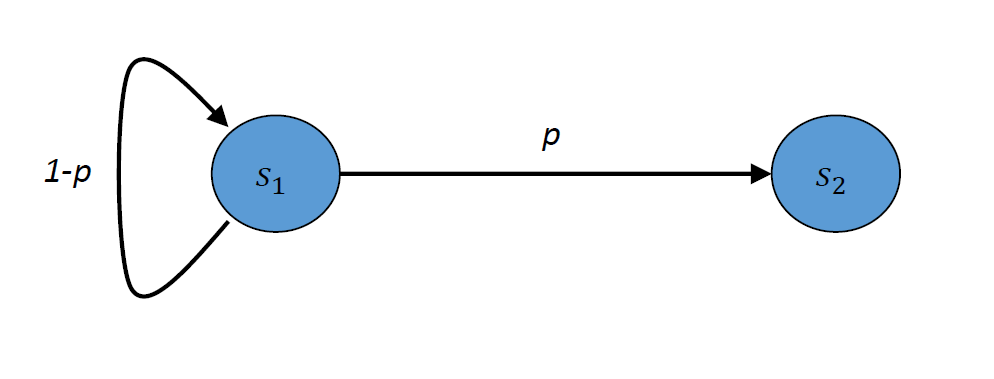
\includegraphics[width=0.5\textwidth]{figures/2state.png}\\
  \caption{The situated agent}\label{fig:2state}
  \end{centering}
\end{figure}

\paragraph{First versus Every visit:}
%
To better understand the difference between first visit and every
visit we consider the following simple test case. We have a two
state MDP, actually a Markov Chain. In the initial state $\state_1$
we have a reward of $1$ and with probability $1-p$ we stay in that
state and with probability $p$ move to the terminating state
$\state_2$. See Figure~\ref{fig:2state}.

The expected value is $\Value(\state_1)=1/p$, which is the expected
length of an episode. (Note that the return of an episode is its
length, since all the rewards are $1$.) Assume we observe a single
trajectory, $(\state_1,\state_1,\state_1,\state_1,\state_2)$, and
all the rewards are $1$. What would be a reasonable estimate for the
expected return from $\state_1$.

{\tt First visit} take the naive approach, considers the return from
the first occurrence of $\state_1$, which is $4$, and uses this as
an estimate. {\tt Every visit} considers four runs from state
$\state_1$, we have:
$(\state_1,\state_1,\state_1,\state_1,\state_2)$ with return $4$,
$(\state_1,\state_1,\state_1,\state_2)$ with return $3$,
$(\state_1,\state_1,\state_2)$ with return $2$, and
$(\state_1,\state_2)$ with return $1$. {\tt Every visit} averages
the four and has $G=(4+3+2+1)/4=2.5$. On the face of it, the
estimate of $4$ seems to make more sense. We will return to this
example later.

\subsection{First visit}
%Maximum likelihood MDP model}

Consider the First Visit Monte-Carlo updates. Assume that for state
$\state$ we have updates $G_1^\state, \ldots , G^\state_m$. Our
estimate would be
$\widehat{\Value}^\policy(\state)=(1/m)\sum_{i=1}^m G^\state_i$.
Since the different $G^\state_i$ are independent, we can use a
concentration bound, to claim that the error is small. Actually we
will need two different bounds. The first would say that if we run
$n$ episodes, then with high probability we have at least $m$
episode in which state $\state$ appear. The second would say that if
we have $m$ episodes in which state $\state$ appear, then we will
well approximate the value function at $\state$. For the first part,
we clearly would need to depend on the probability of reaching state
$\state$ in an episode. Call a state $\state$ as $\alpha$-good if
the probability that $\policy$ visits $\state$ in an episode is at
least $\alpha$.
%This is summarized in t
The following theorem relates the number of episodes to the accuracy
is estimating the value function.
%summarizes the performance of every visit.

\begin{theorem}
Assume that we execute $n$ episodes using policy $\policy$ and each
episode has length at most $H$. Then, with probability $1-\delta$,
for any $\alpha$-good state $\state$, we have
$|\widehat{\Value}^\policy(\state)-\Value^\policy(\state)|\leq
\lambda$, assuming $n\geq (2m/\alpha)\log(2|\States|/\delta)$ and
$m=(H^2/\lambda^2)\log(2|\States|/\delta)$.
\end{theorem}

\begin{proof}
Let $p(\state)$ be the probability that policy $\policy$ visits
state $\state$ in an episode. Since $\state$ is $\alpha$-good, the
expected number of episodes in which $\state$ appears is
$p(\state)n\geq 2m\log(2|\States|/\delta)$. Using the relative
Chernoff--Hoffding bound (Lemma~\ref{lemma:chernoff}) we have that
the probability that we have at least $m$ samples of state $\state$
is at least $1-\delta/(2|\States|)$.

Given that we have at least $m$ samples from state $\state$ using
the additive Chernoff--Hoffding bound (Lemma~\ref{lemma:chernoff})
we have that with probability at least $1-\delta/(2|\States|)$ that
$|\widehat{\Value}^\policy(\state)-\Value^\policy(\state)|\leq
\lambda$. (Since episodes have return in the range $[0,H]$ we need
to normalize by dividing the rewards by $H$, which creates the $H^2$
term in $m$. A more refine bound can be derived by noticing that the
variance of the return of an episode is bounded by $H$ and not
$H^2$, and using an appropriate concentration bound, say Bernstein
inequality.)

Finally, the theorem follows from a union bound over the bad events.
\end{proof}


Next, we relate the First Visit Monte-Carlo updates to the maximum
likelihood model for the MDP. Going back to the example of
Figure~\ref{fig:2state} and observing the sequence
$(\state_1,\state_1,\state_1,\state_1,\state_2)$. The only unknown
parameter is $p$.

The maximum likelihood approach would select the value of $p$ that
would maximize the probability of observing the sequence
$(\state_1,\state_1,\state_1,\state_1,\state_2)$. The likelihood of
the sequence is, $(1-p)^3p$. We like to solve for
\[
p^* = \arg\max (1-p)^3 p
\]
Taking the derivative we have $(1-p)^3-3(1-p)^2p=0$, which give
$p^*=1/4$.
%
For the maximum likelihood (ML) model $M$ we have $p^*=1/4$ and
therefore $V(\state_1;M)=4$.

In general the Maximum Likelihood model value does not always
coincide with the {\tt First Visit} Monte-carlo estimate. However we
can make the following interesting connection.

Clearly, when updating state $\state$ using {\tt First Visit}, we
ignore all the episodes that do not include $\state$, and also for
each the remaining episodes, that do include $\state$, we ignore the
prefix until the fist appearance of $\state$. Let us modify the
sample by deleting those parts (episodes in which $\state$ does not
appear, and for each episode that $\state$ appears, start it at the
first appearance of $\state$). Call this the {\em reduced sample}.
%(For more details, see Theorem 5 in \cite{SinghS96})

The maximum likelihood model, given a set of episodes, is simply the
observed model. (We will not show here that the observed model is
indeed the maximum likelihood model.) Namely, for each state-action
pair $(\state,\action)$ let $n(\state,\action)$ be the number of
times it appears, let $n(\state,\action,\state')$ be the number of
times $\state'$ is observed following executing action $\action$ in
state $\state$. The observed transition model is
$\widehat{p}(\state'|\state,\action)=n(\state,\action,\state')/n(\state,\action)$.
Assume that in the $i$-th execution of action $\action$ in state
$\state$ we observe a reward $\reward_i$ then the observed reward is
$\widehat{\reward}(\state,\action)=(1/n(\state,\action))\sum_{i=1}^{n(\state,\action)}
\reward_i$.

\begin{theorem}
\label{thm:MC-ML}
%
Let $M$ be the maximum likelihood MDP for the reduced sample. The
expected value of $\state_0$ in $M$, i.e., $\Value(\state;M)$, is
identical to the {\tt First Visit} estimate of $\state_0$, i.e.,
$\widehat{\Value}^\policy(\state_0)$.
\end{theorem}

\begin{proof}
Assume that we have $N$ episodes in the reduced sample and the sum
of the rewards in the $i$-th episode is $G_i$. The First Visit Monte
Carlo estimate would be
$\widehat{\Value}^\policy(\state_0)=(1/N)\sum_{i=1}^N G_i$.

Consider the maximum likelihood model. Since we have a fixed
deterministic policy, we can ignore actions, and define
$n(\state)=n(\state,\policy(\state))$ and
$\widehat{\reward}(\state,\policy(\state))=\widehat{\reward}(\state)$.
We set the initial state $\state_0$ to be the state we are updating.

We want to compute the expected number of visits $\mu(\state)$ to
each state $\state$ in the ML model $M$. We will show that
$\mu(\state)=n(\state)/N$. This implies that the expected reward for
state $\state_0$ in $M$ would be
\[
\Value^\policy(\state_0;M)=\sum_v \mu(v) \widehat{r}(v)=\sum_v
\frac{n(v)}{N}\frac{1}{n(v)}\sum_{i=1}^{n(v)} \reward_i^v =
\frac{1}{N}\sum_{j=1}^N G_j
\]
where the last equality follow by changing the order of summation
(from states to episodes).

It remains to show that $\mu(\state)=n(\state)/N$. We have the
following identities. For $v\neq \state_0$:
\[
\mu(v)=\sum_u \widehat{p}(v|u)\mu(u)
\]
For the initial state we have
\[
\mu(\state_0)=1+ \sum_u \widehat{p}(\state_0|u)\mu(u)
\]
Note that $n(v)=\sum_u n(u,v)$ for $v\neq \state_0$ and
$n(\state_0)=N+\sum_u n(u,\state_0)$, and recall that
$\widehat{p}(v|u)=n(u,v)/n(u)$. One can verify the identities by
plugging in these values.
\end{proof}

\subsection{Every visit}

The {\tt First Visit} updates are unbiased, since the different
updates are from different episodes. For each episode that update is
an independent unbiased sample of the return.
%
For {\tt Every Visit} the situation is more complicated, since there
are different updates from the same episode, and therefore they are
dependent. The first issue that we have to resolve is how do we like
to average for the {\tt Every Visit} updates. Let $G^\state_{i,j}$
be the $j$-th update in the $i$-th episode for state $\state$. Let
$n_i$ be the number of updates in episode $i$ and $N$ the overall
number of episodes.

One way to average the updates is to average for each episode the
updates and average across episodes. Namely,
\[
\frac{1}{N}\sum_{i=1}^N \frac{1}{n_i} \sum_{j=1}^{n_i} G_{i,j}
\]
An alternative approach is to sum the updates and divide by the
number of updates,
\[
\frac{\sum_{i=1}^N\sum_{j=1}^{n_i} G_{i,j}}{\sum_{i=1}^N n_i}
\]
We will use the latter scheme, but it is worthwhile understanding
the difference between the two. Consider for example the case that
we have $10$ episodes, in $9$ we have a single visit to $\state$ and
a return of $1$, and in the $10$-th we have $11$ visits to $\state$
and all the returns are zero. The first averaging would give an
estimate of $9/10$ while the second would give an estimate of
$9/20$.

Consider the case of Figure~\ref{fig:2state}. For a single episode
of length $k$ we have that the sum of the rewards is $k(k+1)/2$,
since there are updates of lengths $k, \ldots , 1$ and recall that
the return equals the length since all rewards are $1$. The number
of updates is $k$, so we have that the estimate of a single episode
is $(k+1)/2$. When we take the expectation we have that
$E[(k+1)/2]=(1/p+1)/2$ which is different from the expected value of
$1/p$. (Recall that the {\tt Every Visit} updates $k$ times using
values $k,\ldots,1$. In addition, $E[k]=1/p$ which is also the
expected value.) If we have a single episode then both averaging
schemes are identical.

When we have multiple episodes, we can see the difference between
the two averaging schemes. The first will be biased random variables
of $E[(k+1)/2]=(1/p+1)/2$, so it will converge to this value rather
than $1/p$. The second scheme, which we will use in {\tt Every
Visit} updates, will have the bias decrease with the number of
episodes. The reason is that we sum separately the returns, and the
number of occurrences. This implies that we have
\[
E[\Value^{ev}(\state_1)]=\frac{E[k(k+1)/2]}{E[k]}=\frac{1}{p},
\]
since $E[k^2]=2/p^2-1/p$. This implies that if we average many
episodes we will get an almost unbiased estimate using {\tt Every
Visit}.

We did all this on the example of Figure~\ref{fig:2state}, but this
indeed generalizes. Given an arbitrary episodic MDP, consider the
following mapping. For each episode, mark the places where state
$\state$ appears (the state we want to approximate its value). We
now have a distribution of rewards from going from $\state$ back to
$\state$. Since we are in an episodic MDP, we also have to
terminate, and for this we can add another state, from which we
transition from state $\state$ and have the reward distribution as
the rewards from the last appearance of $\state$ until the end of
the episode.
%We can now reduce collapse other state to a single state.
This implies that we have two states MDP as described in
Figure~\ref{fig:2state-general}.


\begin{figure}
  % Requires \usepackage{graphicx}
  \begin{centering}
  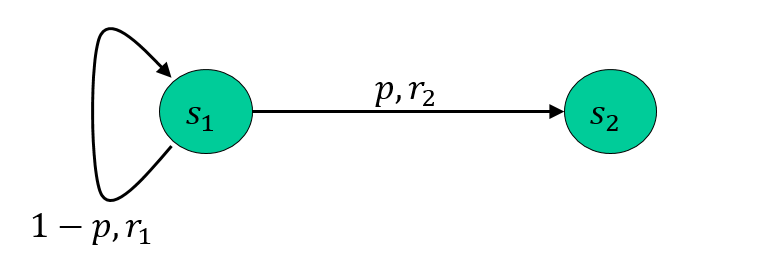
\includegraphics[width=0.5\textwidth]{figures/2state-general.png}\\
  \caption{The situated agent}\label{fig:2state-general}
  \end{centering}
\end{figure}


For this MDP, the value is
$\Value^\pi(\state_1)=\frac{1-p}{p}\reward_1+\reward_2$. The single
episode expected estimate of {\tt Every Visit} is
$\Value^\pi(\state_1)=\frac{1-p}{2p}\reward_1+\reward_2$. The $m$
episodes expected estimate of {\tt Every Visit} is
$V(\state_1)=\frac{m}{m+1}\frac{1-p}{p}\reward_1+\reward_2$. This
implies that if we have a large number of episodes the bias of the
estimate becomes negligible. (For more details, see Theorem 7 in
\cite{SinghS96}.)

\subsubsection*{Every visit and squared loss}

Recall that the squared error is summing over all the observation
the squared error. Assume we have $\state_{i,j}$ as the $j$-th state
in the $i$-th episode, and it has return $G_{i,j}$, i.e., the sum of
the rewards from in episode $i$ from step $j$ until the end of the
episode. Let $\widehat{V}(\state_{i,j})$ be the estimate that {\tt
Every Visit} for state $\state_{i,j}$. (Note that states
$\state_{i,j}$ are not unique, and we can have
$\state=\state_{i_1,j_1}=\state_{i_2,j_2}$.) The square error is
\[
SE=\frac{1}{2}\sum_{i,j} (\widehat{V}(\state_{i,j})-G_{i,j})^2
\]
For a fixed state $\state$ we have
\[
SE(\state)=\frac{1}{2}\sum_{i,j:\state=\state_{i,j}}
(\widehat{V}(\state)-\reward_{i,j})^2
\]
and the total squared error is $SE=\sum_\state SE(\state)$.

Our goal is to select a value $\widehat{V}^{se}(\state)$ for every
state, which would minimize the SE. The minimization is achieved by
minimizing the square error of each $\state$, and setting the values
\[
\widehat{V}^{se}(\state)=\frac{\sum_{i,j:\state=\state_{i,j}}
G_{i,j}}{|{(i,j):\state=\state_{i,j}}|},
\]
which is exactly the {\tt Every Visit} Monte-carlo estimate for
state $\state$.

\subsection{Monte-Carlo control}

We can also use the Monte-Carlo methodology to learn the optimal
policy.
%
The main idea is to learn the $Q^\pi$ function. This is done by
simply updating for every $(\state,\action)$. (The updates can be
either {\tt Every Visit} or {\tt First Visit}.) The problem is that
we need the policy to be ``exploring'', otherwise we will not have
enough information about the actions the policy does not perform.

For the control, we can maintain an estimates of the $Q^\policy$
function, where the current policy is $\policy$. After we have a
good estimate of $Q^\policy$ we can switch to a policy which is
greedy with respect to $Q^\policy$. Namely, each time we reach a
state $\state$, we select a ``near-greedy'' action, for example, use
$\varepsilon$-greedy.

We will show that updating from one $\varepsilon$-greedy policy to
another $\varepsilon$-greedy policy, using policy improvement, does
increase the value of the policy. This will guarantee that we will
no cycle, and eventually converge.

Recall that an $\varepsilon$-greedy policy, can be define in the
following way. For every state $\state$ there is an action
$\bar{\action}_\state$, which is the preferred action. The policy
does the following: (1) with probability $1-\varepsilon$ selects
action $\bar{\action}$. (2) with probability $\varepsilon$, selects
each action $\action \in \Actions$, with probability
$\varepsilon/|\Actions|$.

Assume we have an $\varepsilon$-greedy policy $\policy_1$. Compute
$Q^{\policy_1}$ and define $\policy_2$ to be $\varepsilon$-greedy
with respect to $Q^{\policy_1}$.

\begin{theorem}
For any $\varepsilon$-greedy policy $\policy_1$, the
$\varepsilon$-greedy improvement policy $\policy_2$ has
$\Value^{\policy_2}\geq \Value^{\policy_1}$.
\end{theorem}

\begin{proof}
Let $\bar{\action}_\state=\arg\max_\action
Q^{\policy_1}(\state,\action)$ be the greedy action w.r.t.
$Q^{\policy_1}$. We now lower bound the value of $Q^{\policy_2}$.
\begin{align*}
E_{\action\sim\policy_2(\cdot|\state)}[Q^{\policy_1}(\state,\action)] &= \sum_{\action \in \Actions} \policy_2(\action|\state) Q^{\policy_1}(\state,\action)\\
&= \frac{\varepsilon}{|\Actions|}\sum_{\action \in \Actions}
Q^{\policy_1}(\state,\action)+(1-\varepsilon)Q^{\policy_1}(\state,\bar{\action}_\state)\\
&\geq \frac{\varepsilon}{|\Actions|}\sum_{\action \in \Actions}
Q^{\policy_1}(\state,\action)+(1-\varepsilon)\sum_{\action \in
\Actions}
\frac{\policy_1(\action|\state)-\varepsilon/|\Actions|}{1-\varepsilon}Q^{\policy_1}(\state,\action)\\
&=\sum_{\action \in \Actions} \policy_1(\action|\state)Q^{\policy_1}(\state,\bar{\action})=\Value^{\policy_1}(\state)\\
\end{align*}
The inequality follows, since we are essentially concentrating of
the action that $\policy_1(\cdot|\state)$ selects with probability
$1-\varepsilon$, and clearly $\bar{\action}_\state$, by definition,
guarantees a higher value.

It remains to show, similar to the basic policy improvement, that we
have
$$
\Value^{\policy_2}\geq
%\max_\action Q^{\policy_1}(\state,\action)\geq
E_{\action\sim\policy_2(\cdot|\state)}[Q^{\policy_1}(\state,\action)]
\geq \Value^{\policy_1}.
$$

Basically, we need to re-write the Bellman optimality operator to
apply to $\varepsilon$-greedy policies as follows:
\[
(T^*_\varepsilon V)(\state) = \max_\action
[(1-\varepsilon)(\reward(\state,\action)+\discount E_{\state'\sim
p(\cdot |\state,\action)}[V(\state')])+ \varepsilon
(\sum_{\action''}\frac{\varepsilon}{|\Actions|}(\reward(\state,\action'')
+\discount E_{\state''\sim p(\cdot |s,\action'')}[V(\state'')]))]
\]
Clearly $T^*_\varepsilon(V)$ is monotone in $V$, and for
$\Value^{\policy_1}$ we have
$T^*_\varepsilon(\Value^{\policy_1})=T^{\policy_2}(\Value^{\policy_1})$.
Since $ T^{\policy_2}(\Value^{\policy_1}) =
E_{\action\sim\policy_2(\cdot|\state)}[Q^{\policy_1}(\state,\action)]$,
this implies that,
\[
T^{\policy_2}(\Value^{\policy_1})=T^*_\varepsilon(\Value^\policy_1)
\geq T^{\policy_1}(\Value^{\policy_1}) = \Value^{\policy_1}
\]
We can continue to apply $T^{\policy_2}$ and due to the monotonicity
have
\[
(T^{\policy_2})^k (\Value^{\policy_1}) \geq (T^{\policy_2})^{k-1}
(\Value^{\policy_1}) \geq \cdots \geq \Value^{\policy_1}
\]
Since $\lim_{k\rightarrow \infty}(T^{\policy_2})^k
(\Value^{\policy_1}) = \Value^{\policy_2}$ we are done.
\end{proof}

\subsection{Monte-Carlo: pros and cons}

The main benefits of the Monte-Carlo updates are:
\begin{enumerate}
\item Very simple and intuitive
\item Does not assume the environment is Markovian
\item Extends naturally to function approximation (more in future
chapters)
\item Unbiased updates (using {\tt First Visit}).
\end{enumerate}

\noindent
The main drawback of the Monte-Carlo updates are:
\begin{enumerate}
\item Need to wait for the end of episode to update.
\item Suited mainly for episodic environment.
\item Biased updates (using {\tt Every Visit}).
\end{enumerate}

% %\end{document}
% \newpage
% \section{Temporal Difference algorithms}
\label{sec:TD}


%In this lecture we will continue looking at model-free learning. In
%the previous lecture we presented: (1) $Q$-learning, which is an
%off-policy learning algorithm that learns the optimal $Q^*$
%function, (2) {\tt SARSA} which is an on-policy variant of
%$Q$-learning where we need to select actions, and (3) Monte-Carlo
%which is a model-free algorithm to learn the value function from
%episodes.

In this section we will look on temporal differences methods, which
works in an online fashion. We will start with $TD(0)$ which uses
only the most recent observations for the updates, and we will
continue with methods that allow for a longer look-ahead, and then
consider $TD(\lambda)$ which averages multiple look-ahead
estimations.

In general, temporal differences (TD) methods, learn directly from
experience, and therefore are model-free methods. Unlike Monte-Carlo
algorithms, they will use incomplete episodes for the updates, and
they are not restricted to episodic MDPs. The TD methods update
their estimates given the current observation and in that direction,
similar in spirit to $Q$-learning and SARSA.

\subsection{TD(0)}

Fix a policy $\policy\in \Pi_{SD}$, stationary and deterministic. The goal
is to learn the value function $\Value^\policy(\state)$ for every
$s\in S$. (The same goal as Monte-Carlo learning.) The TD algorithms
will maintain an estimate of the value function of the policy
$\policy$, i.e., maintain an estimate $\widehat{V}_\ttime(\state)$
for $\Value^\policy(\state)$. The TD algorithms will use their
estimates $\widehat{V}$ for the updates. This implies that unlike
Monte-Carlo, there will be an interaction between the estimates of
different states and at different times.

As a starting point, we can recall the {\em value iteration}
algorithm.
\[
V_{\ttime+1}(\state)=E^\policy[\reward(\state,\policy(\state))+\discount
V_\ttime(\state')]
\]
We have shown that value iteration converges, namely $V_\ttime
\rightarrow_{\ttime\rightarrow\infty} \Value^\policy$.

Assume we sample
$(\state_\ttime,\action_\ttime,\reward_\ttime,\state_{\ttime+1})$.
%Assume that $\policy\in SD$, namely a stationary deterministic policy.
Let $\widehat{V}_\ttime$ our estimation at time $\ttime$,
and we sample
$(\state_\ttime,\action_\ttime,\reward_\ttime,\state_{\ttime+1})$.
Then,
\[
E^\policy[\widehat{V}_\ttime(\state_\ttime)]=
E^\policy[\reward_\ttime+\discount
\widehat{V}_\ttime(\state_{\ttime+1})]=E^\policy[\reward(\state,\action)+\discount
\widehat{V}_\ttime(\state')|\state=\state_\ttime,a=\policy(\state)]
\]
%where $E^\policy [\widehat{V}_\ttime]=V_\ttime$.

The $TD(0)$ will do an update in this direction, namely,
$[\reward_\ttime+\discount \widehat{V}_\ttime(\state_{\ttime+1})]$.

\paragraph{$TD(0)$ Algorithm}

\begin{itemize}
\item \emph{Initialize:} $\widehat{V}(\state)$ arbitrarily.

\item At time $\ttime=0,1,\dots$:


-- Observe: $(\state_\ttime, \action_\ttime, \reward_\ttime,
\state_{\ttime+1})$.

-- Update:
%$(\state_\ttime,\action_\ttime,\reward_\ttime,\state_{\ttime+1})$:
\[
\widehat{V}(\state_\ttime)=\widehat{V}(\state_\ttime)+\alpha_\ttime(\state_\ttime,\action_\ttime)
\big[\reward_\ttime+\discount
\widehat{V}(\state_{\ttime+1})-\widehat{V}(\state_\ttime)\big]
\]
where $\alpha_\ttime(\state,\action)$ is the step size for
$(\state,\action)$ at time $\ttime$.
\end{itemize}

We define the {\em temporal difference} to be
\[
\Delta_\ttime =\reward_\ttime+\discount
\widehat{V}(\state_{\ttime+1})-\widehat{V}(\state_\ttime)
\]
The $TD(0)$ update becomes:
\[
\widehat{V}(\state_\ttime)=\widehat{V}(\state_\ttime)+\alpha_\ttime(\state_\ttime,\action_\ttime)\Delta_\ttime
\]


[[YM: motivating example. Waze?!]]

We would like to compare the $TD(0)$ and the Monte-Carlo (MC)
algorithms. Here is a simple example with four states
$S=\{A,B,C,D\}$ where $\{C,D\}$ are terminal states and in $\{A,B\}$
there is one action (essentially, the policy selects a unique
action). Assume we observe eight episodes. One episode is
$(A,0,B,0,C)$, one episode $(B,0,C)$, and six episodes $(B,1,D)$. We
would like to estimate the value function of the non-terminal
states. For $V(B)$ both $TD(0)$ and $MC$ will give $6/8=0.75$. The
interesting question would be: what is the estimate for $A$? MC will
average only the trajectories that include $A$ and will get $0$
(only one trajectory which gives $0$ reward). The $TD(0)$ will
consider the value from $B$ as well, and will give an estimate of
$0.75$. (Assume that the $TD(0)$ continuously updates using the same
episodes until it converges.)

We would like to better understand the above example. For the above
example the empirical MDP will have a transition from $A$ to $B$,
with probability $1$ and reward $0$, from $B$ we will have a
transition to $C$ with probability $0.25$ and reward $0$ and a
transition to $D$ with probability $0.75$ and reward $1$. (See,
Figure~\ref{fig:L7-ML}.) The value of $A$ in the empirical model is
$0.75$. In this case the empirical model agrees with the $TD(0)$
estimate, we show that this holds in general.


\begin{figure}
  % Requires \usepackage{graphicx}
  \begin{centering}
  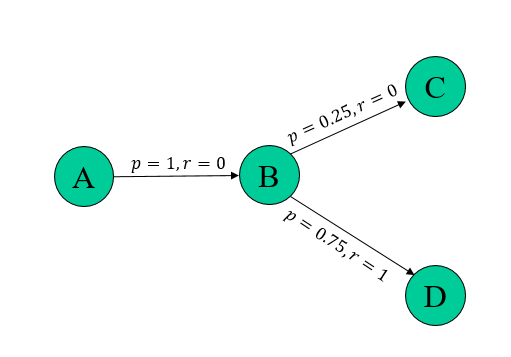
\includegraphics[width=0.5\textwidth]{figures/L7-ML}\\
  \caption{The situated agent}\label{fig:L7-ML}
  \end{centering}
\end{figure}


\paragraph{Maximum Likelihood model}\footnote{YM: repeat} Recall that the empirical model, which is also the
maximum likelihood model, of a sample be define as follows. Let
$n(\state,\action)$ be the number of times $(\state,\action)$
appears in the sample. Given a sample
$(\state_\ttime,\action_\ttime,\reward_\ttime,\state_{\ttime+1})$
for $1\leq t\leq T$, we define the empirical model as follows. The
rewards $\widehat{\reward}(\state,\action)$ are the average rewards
of $(\state,\action)$, i.e.,
$\widehat{\reward}(\state,\action)=\frac{1}{n(\state,\action)}\sum_{\ttime:\state_\ttime=\state,\action_\ttime=\action}\reward_\ttime$
and
$\widehat{p}(\state'|\state,\action)=\frac{n(\state,\action,\state')}{n(\state,\action)}$,
where $n(\state,\action,\state')$ is the number of samples that have
$\state_{\ttime+1}=\state'$ when $\state_\ttime=\state$ and
$\action_\ttime =\action$.

The following theorem states that the value of $\policy$ on the
empirical model is identical to that of $TD(0)$ (running on the
sample until convergence, namely, continuously sampling uniformly
$t\in[1,T]$ and using $(\state_\ttime,
\action_r,\reward_\ttime,\state_{\ttime+1})$ for the $TD(0)$
update).

\begin{theorem}
Let $\Value^\policy_{TD}$ be the estimated value function of
$\policy$ when we run $TD(0)$ until convergence. Let
$\Value^\policy_{EM}$ be the value function of $\policy$ on the
empirical model. Then, $\Value^\policy_{TD}=\Value^\policy_{EM}$.
\end{theorem}

\begin{proof}[Proof sketch]
The update of $TD(0)$ is
$\widehat{V}(\state_\ttime)=\widehat{V}(\state_\ttime)+\alpha_\ttime(\state_\ttime,\action_\ttime)\Delta_\ttime$,
where $\Delta_\ttime=\reward_\ttime+\discount
\widehat{V}(\state_{\ttime+1})-\widehat{V}(\state_\ttime)$. At
convergence we have $E[\Delta_\ttime]=0$ and hence,
\[
\widehat{V}(\state)=\frac{1}{n(\state,\action)}\sum_{\state_{\ttime+1}:\state_\ttime=\state,\action_\ttime=\action}
\reward_\ttime+\discount
\widehat{V}(\state_{\ttime+1})=\widehat{\reward}(\state,\action)+\discount
E_{\state'\sim
\widehat{p}(\cdot|\state,\action)}[\widehat{V}(\state')]
\]
where $\action=\policy(\state)$.
\end{proof}

In is worth to compare the above theorem to the case of Monte Carlo
(Theorem~\ref{thm:MC-ML}). Here we are using the entire sample, and
we have the same ML model for any state $\state$. In the Monte-Carlo
case we used a reduced sample, which depends on the state $\state$
and therefore we have a different ML model for each state, based on
its reduced sample.

\paragraph{Convergence:} The proof of the convergence of $TD(0)$ is very
similar to that of $Q$-learning. We will show that $TD(0)$ is an
instance of the stochastic approximation algorithm, as presented in
previously in Section~\ref{sec:stochastic-approximation}, and the
convergence proof will follow from this.
%We will first state it.

\begin{theorem}[Convergence $TD(0)$]
\label{thm:TD0-conrg} If the step size has the properties that for
every $(\state,\action)$ we have $\sum_\ttime
\alpha_\ttime(\state,\action)=\infty $ and $\sum_\ttime
\alpha_\ttime^2(\state,\action)=O(1)$, then $\widehat{V}$ converges
to $\Value^\policy$, with probability $1$.
\end{theorem}

We will show the convergence using the general theorem for
stochastic approximation iterative algorithm
(Theorem~\ref{thm:stoch-approx}).

We first define a linear operator $H$ for the policy $\policy$,
\[
(Hv)(\state)=\reward(\state,\policy(\state))+\discount\sum_{\state'}p(\state'|\state,\policy(\state))v(\state')
\]
Note that $H$ is the operator $T^\policy$ we define in
Section~\ref{ss:DP_op}.

As we saw before, the operator $H$ is a $\discount$-contracting
operator
\begin{align*}
\|Hv_1-Hv_2\|_\infty &= \discount \max_{s} |
\sum_{\state'}p(\state'|\state,\policy(\state))(v_1(\state')-v_2(\state'))|\\
&\leq \discount\max_{\state'} |v_1(\state')-v_2(\state')|\\
&\leq \discount \|v_1-v_2\|_\infty
\end{align*}
%Therefore $H$ is $\discount$-contracting.

We now would like to re-write the $TD(0)$ update to be a stochastic
approximation iterative algorithm. The $TD(0)$ update is,
\[
V_{\ttime+1}(\state_\ttime)=(1-\alpha_\ttime)V_\ttime(\state_\ttime)+\alpha_\ttime
\Phi_\ttime
\]
where $\Phi_\ttime=\reward_\ttime+\discount
V_\ttime(\state_{\ttime+1})$. We would like to consider the expected
value of $\Phi_\ttime$. Clearly,
$E[\reward_\ttime]=\reward(\state_\ttime,\policy(\state_\ttime))$
and $\state_{\ttime+1} \sim p(\cdot |\state_\ttime,\action_\ttime)$.
This implies that $E[\Phi_\ttime]=(HV_\ttime)(\state_\ttime)$.
Therefore, we can define the noise term $\omega_\ttime$ as follows,
\[
\omega_\ttime(\state_\ttime)=[\reward_\ttime+\discount
V_\ttime(\state_{\ttime+1})]-(HV_\ttime)(\state_\ttime)\;,
\]
and have $E[\omega_\ttime]=0$. We can bound $|\omega_\ttime|\leq
V_{max}=\frac{R_{max}}{1-\discount}$, since the value function is
bounded by $V_{max}$.

Returning to $TD(0)$, we can write
\[
V_{\ttime+1}(\state_\ttime)=(1-\alpha_\ttime)V_\ttime(\state_\ttime)+\alpha_\ttime
[(HV_\ttime)(\state_\ttime)+\omega_\ttime(\state_\ttime)]
\]
The requirement of the step size appears in the statement of the
theorem (and so holds). The noise $\omega_\ttime$ has both
$E[\omega_\ttime]=0$ and $|\omega_\ttime|\leq V_{max}$. And the
operator $H$ is contracting with a fix-point $\Value^\policy$.
Therefore, using Theorem~\ref{thm:stoch-approx}, we established
Theorem~\ref{thm:TD0-conrg}.

\paragraph{Comparing various algorithms:}\footnote{YM: needed? I think it is from Sutton}
When we compare $TD(0)$, to $MC$ and both to  Dynamic Programming
(DP) we can view it as different ways of computing the value
function.
\begin{itemize}
\item[MC] We have $\Value^\policy(\state)=E[R_\ttime|\state_\ttime=\state]$. In MC we observe the
return, $R_\ttime$, of episodes, and their mean is what we like to
estimate.
\item [$TD(0)$]  We have $\Value^\policy(\state)=E[\reward_\ttime+\discount \Value^\policy(\state_{\ttime+1})|\state_\ttime=\state]$. In $TD(0)$ we observe samples of
$\reward_\ttime$, we use our estimate for
$\Value^\policy(\state_{\ttime+1})$ and the expectation is what we
like to estimate (assuming our estimates converge).
\item
[DP]
 We have $\Value^\policy(\state)=\sum_{\action}\policy(\action|\state)[\reward(\state,\action)+\discount \sum_{\state'}p(\state'|\state,\action)\Value^\policy(\state')]$. In DP we
 have the entire model, and use it to compute expectations.
\end{itemize}

We can see the difference between $TD(0)$ and $MC$ in the Markov
Chain in Figure~\ref{fig:L7-TD-MC}. To get an approximation of state
$\state_2$, i.e., $|\widehat{V}(\state_2)-\frac{1}{2}|\approx
\varepsilon$. The Monte-Carlo will require $O(1/(\beta
\varepsilon^2))$ episodes (out of which only $O(1/\varepsilon^2)$
start at $\state_2$) and the $TD(0)$ will require only
$O(1/\varepsilon^2+1/\beta)$ since the estimate of $\state_3$ will
converge after $1/\varepsilon^2$ episodes which start from
$\state_1$.

\begin{figure}
  % Requires \usepackage{graphicx}
  \begin{centering}
  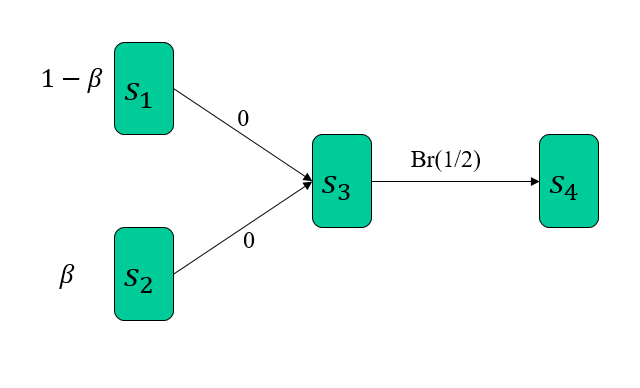
\includegraphics[width=0.5\textwidth]{figures/L7-TD-MC}\\
  \caption{Markov Reward Chain}\label{fig:L7-TD-MC}
  \end{centering}
\end{figure}


\subsection{TD: Multiple look-ahead}

The $TD(0)$ uses only the current reward and state. Given
$(\state_\ttime,\action_\ttime,\reward_\ttime,\state_{\ttime+1})$ it
updates $\Delta_\ttime=R^{(1)}_\ttime(\state_\ttime) -
\widehat{V}(\state_\ttime)$ where $R^{(1)}_\ttime(\state_\ttime)=
\reward_\ttime +\discount \widehat{V}(\state_{\ttime+1})$. We can
also consider a two step look-ahead as follows. Given
$(\state_\ttime,\action_\ttime,\reward_\ttime,\state_{\ttime+1},\action_{\ttime+1},\reward_{\ttime+1},\state_{\ttime+2})$
we can update using
$\Delta^{(2)}_\ttime=R^{(2)}_\ttime(\state_\ttime) -
\widehat{V}(\state_\ttime)$ where $R^{(2)}_\ttime(\state_\ttime)=
\reward_\ttime+\discount \reward_{\ttime+1} +\discount^2
\widehat{V}(\state_{\ttime+2})$. Using the same logic, we have that
this is a temporal difference that uses a two time steps.

We can generalize this to any $n$-step look-ahead and define
$R^{(n)}_\ttime(\state_\ttime)= \sum_{i=0}^{n-1} \discount^i
\reward_{\ttime+i}+\discount^n \widehat{V}(\state_{\ttime+n})$ and
updates $\Delta^{(n)}_\ttime=R^{(n)}_\ttime(\state_\ttime) -
\widehat{V}(\state_\ttime)$.

We can relate the $\Delta^{(n)}_\ttime$ to the $\Delta_\ttime$ as
follows:
\[
\Delta^{(n)}_\ttime=\sum_{i=0}^{n-1} \discount^i \Delta_{\ttime+i}
\]
This follows since
\[
\sum_{i=0}^{n-1} \discount^i \Delta_{\ttime+i}=\sum_{i=0}^{n-1}
\discount^i \reward_{\ttime+i}+ \sum_{i=0}^{n-1} \discount^{i+1}
\widehat{V}(\state_{\ttime+i+1})- \sum_{i=0}^{n-1} \discount^{i}
\widehat{V}(\state_{\ttime+i})=\sum_{i=0}^{n-1} \discount^i
\reward_{\ttime+i}+\discount^n
\widehat{V}(\state_{\ttime+n})-\widehat{V}(\state_\ttime)
\]

Using the $n$-step look-ahead we have
$\widehat{V}(\state_\ttime)=\widehat{V}(\state_\ttime)+\alpha_\ttime
\Delta^{(n)}_\ttime$ where
$\Delta^{(n)}_\ttime=R^{(n)}_\ttime(\state_\ttime)-\widehat{V}(\state_\ttime)$.
We can view $R^{(n)}_\ttime$ as an operator over $V$, and this operator is
%Note that the operator $R^{(n)}_\ttime$ is
$\discount^n$-contracting, namely
\[
\| R^{(n)}_\ttime(V_1)-R^{(n)}_\ttime(V_2)\|_\infty \leq \discount^n
\|V_1-V_2\|_\infty
\]

We can use any parameter $n$ for the $n$-step look-ahead. If the
episode ends before step $n$ we can pad it with rewards zero. This
implies that for $n=\infty$ we have that $n$-step look-ahead is
simply the Monte-Carlo estimate. However, we need to select some
parameter $n$. An alternative idea is to simply average over the
possible parameters $n$. One simple way to average is to use
exponential averaging with a parameter $\lambda\in(0,1)$. This
implies that the weight of each parameter $n$ is
$(1-\lambda)\lambda^{n-1}$.

This leads us to the $TD(\lambda)$ update:
\[
\widehat{V}(\state_\ttime)=\widehat{V}(\state_\ttime)+\alpha_\ttime(1-\lambda)\sum_{n=1}^\infty
\lambda^{n-1}\Delta^{(n)}_\ttime
\]

\noindent{\bf Remark:} While both $\discount$ and $\lambda$ are used
to generate exponential decaying values, their goal is very
different. The discount parameter $\discount$ defines the objective
of the MDP, the goal that we like to maximize. The exponential
averaging parameter $\lambda$ is used by the learning algorithm to average over the different
look-ahead parameters, and is selected to optimize the convergence.

%In the slides there is an example of a random walk and its
%convergence taken from \cite{SuttonB98}.

The above describes the forward view of $TD(\lambda)$, where we
average over future rewards. If we will try to implement it in a
strict way this will lead us to wait until the end of the episode,
since we will need to first observe all the rewards. Fortunately,
there is an equivalent form of the $TD(\lambda)$ which uses a {\em
backward view}. The backward view updates at each time step, using
an incomplete information. At the end of the episode, the updates of
the forward and backward updates will be the same.

The basic idea of the backward view is the following. Fix a time
$\ttime$ and a state $\state=\state_\ttime$. We have at time
$\ttime$ a temporal difference $\Delta_\ttime= \reward_\ttime
+\discount V_\ttime(\state_{\ttime+1})-V_\ttime(\state_\ttime)$.
Consider how this $\Delta_\ttime$ affects all the previous times
$\tau<\ttime$ where $\state_\tau=\state=\state_\ttime$. The influence is
exactly $(\discount\lambda)^{\ttime-\tau}\Delta_\ttime$. This implies
that for every such $\tau$ we can do the desired update, however, we
can aggregate all those updates to a single update. Let,
\[
e_\ttime(\state)=\sum_{\tau\leq \ttime: \state_\tau=\state}
(\discount\lambda)^{\ttime-\tau} = \sum_{\tau=1}^\ttime
(\discount\lambda)^{\ttime-\tau}I(\state_\tau=\state)
\]
The above $e_\ttime(\state)$ defines the {\em eligibility trace} and
we can compute it online using
\[
e_\ttime(\state)=\discount\lambda
e_{\ttime-1}(\state)+I(\state=\state_\ttime)
\]
which result in the update
\[
\widehat{V}_{\ttime+1}(\state)=\widehat{V}_\ttime(\state)+\alpha_\ttime
e_\ttime(\state)\Delta_\ttime
\]
Note that for $TD(0)$ we have that $\lambda=0$ and the eligibility
trace becomes $e_\ttime(\state)=I(\state=\state_\ttime)$. This
implies that we update only $\state_\ttime$ and
$\widehat{V}_{\ttime+1}(\state_\ttime)=\widehat{V}_\ttime(\state_\ttime)+\alpha_\ttime
\Delta_\ttime$.

\paragraph{$TD(\lambda)$ algorithm}\ \\

 -- Initialization: Set $\widehat{V}(\state)=0$ (or any other value), and
 $e_0(\state)=0$.

 -- Update: observe $(\state_\ttime,\action_\ttime,\reward_\ttime,\state_{\ttime+1})$ and set
\begin{align*}
\Delta_\ttime &= \reward_\ttime +\discount \widehat{V}_\ttime(\state_{\ttime+1})-\widehat{V}(\state_\ttime)\\
e_\ttime(\state) &= \discount\lambda e_{\ttime-1}(\state)+I(\state=\state_\ttime)\\
\widehat{V}_{\ttime+1}(\state) &=
\widehat{V}_\ttime(\state)+\alpha_\ttime e_\ttime
(\state)\Delta_\ttime
\end{align*}

 To summarize, the
benefit of $TD(\lambda)$ is that it interpolates between $TD(0)$ and
Monte-carlo updates, and many times achieves superior performance to
both.
%
Similar to $TD(0)$, also  $TD(\lambda)$ can be written as a
stochastic approximation iterative algorithm, and one can derive its
convergence.
%
In the next section we show the equivalence of the forward and
backward $TD(\lambda)$ updates.
%

\subsection{The equivalence of the forward and backward view}

We would like to show that indeed the forward and backward view
result in the same overall update.

For the forward view we define the updates to be
$\Delta^F_\ttime(\state)=\alpha(R^\lambda_\ttime-V_\ttime(\state))$,
where $R^\lambda_\ttime=(1-\lambda)\sum_{n=1}^\infty
\lambda^{n-1}R_\ttime^{(n)}$. Equivalently,
$\Delta^F_\ttime(\state)=\alpha (1-\lambda)\sum_{n=1}^\infty
\Delta_\ttime ^{(n)}$.


For the backward view we define the updates to be
$\Delta^B_\ttime(\state)=\alpha\Delta_\ttime e_\ttime(\state)$,
where the eligibility trace is
$e_\ttime(\state)=\sum_{k=0}^\ttime(\lambda\discount)^{\ttime-k}I(\state=\state_k)$.

\begin{theorem}
%For any trajectory of length $T$ we have
\[
\sum_{\ttime=0}^{\infty} \Delta V ^B_\ttime
(\state)=\sum_{\ttime=0}^{\infty} \Delta V_\ttime^F(\state)
I(\state_\ttime=\state)
\]
\end{theorem}

\begin{proof}
Consider the sum of the forward updates for state $\state$:
\begin{align}
\sum_{\ttime=0}^{\infty } \Delta \Value^F_\ttime (\state)&=
\sum_{\ttime=0}^{\infty} \alpha
(1-\lambda) \sum_{n=\ttime}^{\infty} \lambda^{n-\ttime}\Delta_\ttime^{(n)} I(\state=\state_\ttime)\nonumber\\
%
&= \sum_{\ttime=0}^{\infty}  \alpha
(1-\lambda) \sum_{n=\ttime}^{\infty} \lambda^{n-\ttime}\sum_{i=0}^n \discount^i \Delta_{\ttime+i} I(\state=\state_\ttime)\nonumber\\
%
&=\sum_{\ttime=0}^\infty \sum_{n=0}^\infty \sum_{k=\ttime}^n \alpha
(1-\lambda)
\lambda^{n-k}\lambda^{k-\ttime}\discount^{k-\ttime}\Delta_k I(\state=\state_\ttime)\nonumber\\
%
&=\sum_{\ttime=0}^\infty \sum_{k=\ttime}^\infty \alpha
(\discount\lambda)^{k-\ttime}\Delta_k I(\state=\state_\ttime) \sum_{i=0}^\infty (1-\lambda)\lambda^{i}\nonumber\\
%
&= \sum_{\ttime=0}^\infty \sum_{k=\ttime}^\infty \alpha
(\discount\lambda)^{k-\ttime} \Delta_k(\state)
I(\state=\state_\ttime) \label{eq:TD-F}
\end{align}
where the first identity is the definition, the second identity
follows since $\Delta_\ttime^{(n)}=\sum_{i=0}^n\discount^i
\Delta_{\ttime+i}$, in the third identity we substitute $k$ for
$\ttime+i$ and sum over $n$, $k$ and $\ttime$, in the forth identity we
substitute $i$ for $n-k$ and isolate the terms that depend on $i$,
and in the last identity we note that $\sum_{i=0}^\infty
(1-\lambda)\lambda^{i}=1$.

For the backward view for state $\state$ we have
\begin{align}
\sum_{\ttime=0}^{\infty } \Delta \Value^B_\ttime (\state)&=\sum_{\ttime=0}^{\infty} \alpha
\Delta_\ttime(\state) e_{\ttime}(\state)\\
\sum_{\ttime=0}^{\infty} \alpha
\Delta_\ttime(\state) \sum_{k=0}^\ttime (\discount\lambda)^{\ttime-k} I(\state=\state_\ttime)\nonumber\\
&= \sum_{k=0}^\infty \sum_{\ttime=k}^\infty \alpha
(\discount\lambda)^{\ttime-k}\Delta_\ttime(\state)I(\state=\state_\ttime)
\label{eq:TD-B}
\end{align}

Note that if we interchange $k$ and $\ttime$ in Eq. (\ref{eq:TD-F})
and in Eq. (\ref{eq:TD-B}), then we have the identical expressions.
\end{proof}

\subsection{$SARSA(\lambda)$}

We can use the idea of eligibility traces also in other algorithms,
such as SARSA. Recall that given
$(\state_\ttime,\action_\ttime,\reward_\ttime,\state_{\ttime+1},\action_{\ttime+1})$
the update of SARSA is
\[
\reward_\ttime+\discount
Q_\ttime(\state_{\ttime+1},\action_{\ttime+1})-Q_\ttime(\state_\ttime,\action_\ttime)
\]
Similarly, we can define an $n$-step look-ahead
$q^{(n)}_\ttime=\sum_{i=0}^{n-1}\discount^i \reward_{\ttime+i}
+\discount^n Q_\ttime(\state_{\ttime+n},\action_{\ttime+n})$ and set
$Q_{\ttime+1}(\state_\ttime,\action_\ttime)=Q_\ttime(\state_\ttime,\action_\ttime)+\alpha_\ttime
(q^{(n)}_\ttime-Q_\ttime(\state_\ttime,\action_\ttime))$.

We can now define $SARSA(\lambda)$ using exponential averaging with
parameter $\lambda$. Namely, we define
$q^\lambda_\ttime=(1-\lambda)\sum_{n=1}^\infty
\lambda^{n-1}q^{(n)}_{\ttime}$. This makes the forward view of
$SARSA(\lambda)$ to be
$Q_{\ttime+1}(\state_\ttime,\action_\ttime)=Q_\ttime(\state_\ttime,\action_\ttime)+\alpha_\ttime
(q^{\lambda}_\ttime-Q_\ttime(\state_\ttime,\action_\ttime))$.


Similar to $TD(\lambda)$, we can define a backward view using
eligibility traces:
\begin{align*}
e_0(\state,\action)&=0\\
e_\ttime(\state,\action)&=\discount\lambda
e_{\ttime-1}(\state,\action)+ I(\state=\state_\ttime,
a=\action_\ttime)
\end{align*}
For the update we have
\begin{align*}
\Delta_\ttime&= \reward_\ttime +\discount Q_\ttime(\state_{\ttime+1},\action_{\ttime+1})-Q_\ttime(\state_\ttime,\action_\ttime)\\
Q_{\ttime+1}(\state,\action)&=Q_{\ttime}(\state,\action)+\alpha_\ttime
e_\ttime(\state,\action)\Delta_\ttime
\end{align*}

\section{Miscellaneous}

\subsection{Importance Sampling}

Importance sapling is a simple general technique to estimate the
mean with respect to a given distribution, while sampling from a
different distribution. To be specific, let $Q$ be the sampling
distribution and $P$ the evaluation distribution. The basic idea is
the following
\[
E_{x\sim P}[f(x)]=\sum_x P(x)f(x)=\sum_x Q(x)\frac{P(x)}{Q(x)}
f(x)=E_{x\sim Q} [\frac{P(x)}{Q(x)}f(x)]
\]
This implies that given a sample $\{x_1, \ldots , x_m\}$ from $Q$,
we can estimate $E_{x\sim P}[f(x)]$ using $\sum_{i=1}^m
\frac{P(x_i)}{Q(x_i)}f(x_i)$.

The importance sampling gives an unbiased estimator, but the
variance of the estimator might be huge, since it depends on
$P(x)/Q(x)$.

We would like to apply the idea of importance sampling to learning
in MDPs. Assume that there is a policy $\policy$ that selects the
actions, and there is a policy $\rho$ that we would like to
evaluate. For the importance sampling, given a trajectory, we need
to take the ratio of probabilities under $\rho$ and $\policy$.
\[
\frac{\rho(\state_1,\action_1,\reward_1,
\ldots,\state_{T},\action_{T},\reward_T,\state_{T+1})}{\policy(\state_1,\action_1,\reward_1,
\ldots,\state_{T},\action_{T},\reward_T,\state_{T+1})}=\prod_{\ttime=1}^T
\frac{\rho(a_\ttime|\state_\ttime)}{\policy(a_\ttime|\state_\ttime)}
\]
where the equality follows since the reward and transition
probabilities are identical, and cancel.

For Monte-Carlo, the estimates would be
\[
G^{\rho/\policy}=\prod_{\ttime=1}^T
\frac{\rho(\action_\ttime|\state_\ttime)}{\policy(\action_\ttime|\state_\ttime)}
(\sum_{\ttime=1}^T \reward_\ttime)
\]
and we have
\[
\widehat{V}^\rho (\state_1) = \widehat{V}^\rho(\state_1) +\alpha(
G^{\rho/\policy}- \widehat{V}^\rho(\state_1))
\]
This updates might be huge, since we are multiplying the ratios of
many small numbers.

For the $TD(0)$ the updates will be
\[
\Delta^{\rho/\policy}_\ttime
=\frac{\rho(\action_\ttime|\state_\ttime)}{\policy(\action_\ttime|\state_\ttime)}\reward_\ttime
+\discount \widehat{V}(\state_{\ttime+1})-\widehat{V}(\state_\ttime)
\]
and we have
\[
\widehat{V}^\rho (\state_1) = \widehat{V}^\rho(\state_1) +\alpha(
\Delta^{\rho/\policy}_\ttime- \widehat{V}^\rho(\state_1))
\]
This update is much more stable, since we have only one factor
multiplying the observed reward.


\subsection{Actor-critic methodology}


Actor-critic gives a general methodology of building reinforcement
learning algorithms. It is composed from an actor, that selects the
actions, and a critic, that learns the value function. The actor
observes the current state, and the value function, and selects an
action. The critic, observes the current state (and action) and
reward and outputs a value function. See
Figure~\ref{fig:L7-Actor-Critic}.

\begin{figure}
  % Requires \usepackage{graphicx}
  \begin{centering}
  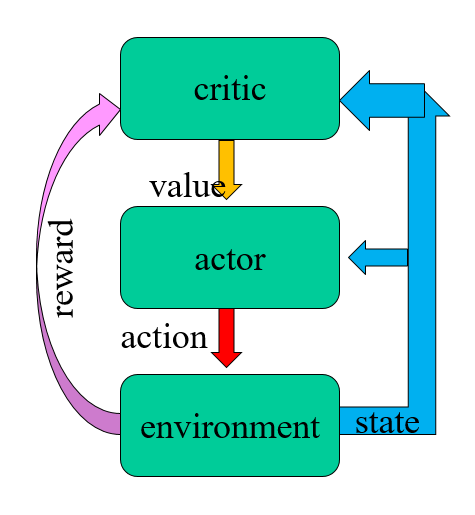
\includegraphics[width=0.5\textwidth]{figures/L7-Actor-Critic}
  \caption{The situated agent}\label{fig:L7-Actor-Critic}
  \end{centering}
\end{figure}





\section{Bibliography Remarks}

The $Q$-learning outline of the asymptotic convergence and the step
size analysis follows \cite{Even-DarM03}.

Expected SARSA was presented in \cite{SeijenHWW09}

The comparison of the {\tt First Visit} and {\tt Every Visit} is
based on \cite{SinghS96}.

Part of the outline borrows from David Silver class notes and the
the book of Sutton and Barto \cite{SuttonB98}.


The presentation of the TD algorithms follows the book of Sutton and
Barto \cite{SuttonB98}.

% %\input{exercises7}

% \chapter{Tabular learning: off-policy}
% %\input{Lecture10}

% \chapter{Large state space: value function approximation}
% This chapter starts looking at the case where the MDP models are
large. In the current chapter we will look at approximating the
value function. In the next chapter we will consider learning
directly a policy and optimizing it.

When we talk about a large MDP, it can be in one of a few different
reasons. The most common is having a large state space. For example,
Backgammon has $10^{20}$ states, Go has $10^{170}$ and robot control
has continuous state space. Another dimension is the action space,
which can be even continuous in many applications (say, robots).
Finally, we might have a complex dynamics which are hard to describe
succinctly. The main challenge is that we need our algorithm to
scale up to this enormous spaces.

 Previously, we had a look-up table for the value
function $\Value^\policy(\state)$ or $Q^\policy(\state,\action)$,
which we updated every time we encountered the state $\state$.
%
Here, we will consider function approximation for large MDPs, mainly
large state spaces.
%
In a large state space this will be infeasible. Not only that we do
not have the memory, but even more importantly, we are unlikely to
observe states re-occurring. We will need to make (implicit)
assumptions about the MDP, which can be viewed similarly to our
assumption in learning a classifier in supervised learning.

Specifically, we will have the value functions parameterized by {\em
weights} $\weight$, namely, $\widehat{V}(\state;\weight)\approx
\Value^\policy(\state)$ and
$\widehat{Q}(\state,\action;\weight)\approx
Q^\policy(\state,\action)$. We would like to guarantee
generalization from the observed states and trajectories to
unobserved states and trajectories. In the process we will update
the weights $\weight$, using some learning procedure, most notably
using MC or TD learning.

When considering a value function there are a few interpretations
what exactly we mean. It can either be: (1) mapping from a state
$\state$ to its expected return, i.e.,
$\widehat{V}^\policy(\state;\weight)$. (2) mapping from state-action
pairs $(\state,\action)$ to their expected return, i.e.,
$\widehat{Q}^\policy(\state,\action;\weight)$. (3) mapping from
states $\state$ to expected return of each action, i.e.,
$\langle\widehat{Q}^\policy(\state,\action_i;\weight):\action_i\in
\Actions\rangle$. All the interpretations are valid, and our
discussion will not distinguish between them. (Actually, for
$\langle\widehat{Q}^\policy(\state,\action_i;\weight):\action_i\in
\Actions\rangle$ we implicitly assume that the number of actions is
small.)

We now need to discuss how will we build the approximating function.
For this we can turn to the rich literature in Machine Learning and
consider popular hypothesis classes. For example: (1) Linear
functions, (2) Neural networks, (3) Decision trees, (4) Nearest
neighbors, (5) Fourier or wavelet basis, etc. We will concentrate
here on linear functions and neural networks, mainly since gradient
based methods apply to them very naturally.

We will consider in this chapter (mainly) the discounted return with
a discount parameter $\gamma\in(0,1)$. The results extend very
naturally to the finite horizon and episodic settings.

\textbf{YM: Maybe better to switch to finite horizon, and avoid the
need for mixing time and stead state distribution?}

\section{Basic Approximation}

Before we start the discussion on the learning methods, we will do a
small detour. We will discuss the effect of having an error in the
value function we learn, and its effect on the outcome. Assume we
have a value function $V$ such that $\|V-\Value^*\|_\infty\leq
\varepsilon$. Let $\policy$ be the greedy policy with respect to
$V$, namely,
\[
\policy(\state)=\arg\max_\action [\reward(\state,\action)+\gamma
E_{\state'\sim p(\cdot|\state,\action)}[V(\state')]
\]


\begin{theorem}
Let $V$ such that $\|V-\Value^*\|_\infty\leq \varepsilon$ and
$\policy$ be the greedy policy with respect to $V$. Then,
\[
\|\Value^\policy-\Value^*\|_\infty\leq\frac{2\gamma\varepsilon}{1-\gamma}
\]
\end{theorem}

\begin{proof}
Consider two operators $\operator^\policy$ and $\operator^*$ (see
Chapter \ref{ss:DP_op}). The first $\operator^\policy$ is
\[
(\operator^\policy v)(\state)=\reward(\state,\policy(\state))+\gamma
E_{\state'\sim p(\cdot|\state,\policy(\state))}[v(\state')],
\]
and it converges to $\Value^\policy$ (see Theorem~\ref{thm:DP_op}).


The second $T^*$ is
\[
(\operator^* v)(\state)=\max_\action[\reward(\state,\action)+\gamma
E_{\state'\sim p(\cdot|\state,\action)}[v(\state')] ],
\]
and it converges to $\Value^*$ (see Theorem~\ref{thm:DP_op}).

In addition, recall that we have showed that both
$\operator^\policy$ and $\operator^*$ are $\gamma$-contracting (see
Theorem~\ref{thm:DP_op}).

Since $\policy$ is greedy with respect to $V$ we have
$\operator^\policy V=\operator^* V$ (but this does not hold for
other value functions $V'$).

Then,
\begin{align*}
\|\Value^\policy-\Value^*\|_\infty &= \|T^\policy \Value^\policy - \Value^*\|_\infty\\
&\leq \|T^\policy \Value^\policy -T^\policy V\|_\infty +\|T^\policy V - \Value^*\|_\infty\\
&\leq \gamma\| \Value^\policy - V\|_\infty +\|T^* V - T^*\Value^*\|_\infty\\
&\leq \gamma\| \Value^\policy - V\|_\infty +\gamma\| V - \Value^*\|_\infty\\
&\leq \gamma(\| \Value^\policy - \Value^*\|_\infty+ \|\Value^*-V\|_\infty ) +\gamma\| V - \Value^*\|_\infty\;,
\end{align*}
where in the second inequality we used the fact that since since
$\policy$ is greedy with respect to $V$ then $T^\policy V=T^* V$.

Reorganizing the inequality and recalling that
$\|\Value^*-\Value\|_\infty\leq \varepsilon$, we have
\[
(1-\gamma)\|\Value^\policy-\Value^*\|_\infty \leq 2\varepsilon\gamma
\]
and the theorem follows.
\end{proof}

The above theorem states that if we have a small errors in
$L_\infty$ norm, the effect of the errors on the expected return is
bounded. However, in most cases we will not be able to guarantee an
approximation in norm $L_\infty$. This is since it is infeasible even
to compute the $L_\infty$ norm of two given value function, since
this requires considering {\em all} states. In the large state space
setting such operations are infeasible.

\section{From RL to ML}

We would like to reduce our reinforcement learning problem to a
supervised learning problem. This will enable us to use any of the
many techniques of machine learning to address the problem. Let us
consider the basic ingredients of supervised learning. The most
important ingredient is having a labeled sample set, which is
sampled i.i.d.

Let us start by considering an idealized setting. Fix a policy
$\policy$ that we like to learn its value function. We like to
generate a sample
\[
\{(\state_1, \Value^\policy(\state_1)),\ldots,
(\state_m,\Value^\policy(\state_m))\}
\]
We first need to discuss how to sample the states $\state_i$ in an
i.i.d. way. We can generate trajectory, but we need to be careful,
since adjacent states are definitely dependent! One solution is to
space the sampling from the trajectory using the mixing time of
$\policy$.\footnote{See Chapter \ref{chapter:MC} for definition.}
This will give us samples $\state_i$ which are (almost) from the
stationary distribution of $\policy$ and are (almost) independent.
%For the action, we clearly will use $\policy$, no problem there.

The hardest, and most confusing, ingredient is the labels
$\Value^\policy(\state_i)$. In machine leaning we actually assume
that someone gives us the labels to build a classifier.
% (or alternatively, in unsupervised learning, where there is no clear ground truth).
If someone is able to give us
$\Value^\policy(\state)$, it seems like assuming the problem away,
since this is what we would like to learn.

Actually we need to define three things: (1) sample states and actions,
which we will do using $\policy$, (2) a loss function, which will
give the tradeoffs between different approximation errors, and (3)
labels, which we are not given explicitly.

For the state and actions we will define a threshold $\tau$, which
will depends on the mixing time. We will run the policy $\policy$
for $\tau$ steps and then output the state $\state$ (and action
$\action$, if needed).

For the loss function we will define a differential loss function
$J(\weight)$. This will enable us to compute the gradient of the
loss function $\nabla_\weight
J(\weight)=\langle\frac{\partial}{\partial \weight_1}J(\weight),
\ldots , \frac{\partial}{\partial \weight_d}J(\weight)\rangle$, and
update the weights in the negative direction of the gradient,
namely, $\Delta \weight=-\alpha\nabla_\weight J(\weight)$, where
$\alpha$ is the step size of the learning rate. In supervised
learning we are guaranteed that the process will converge to a local
minimum (or a saddle point).

Let us start by defining the loss function,
\[
J(\weight)=\frac{1}{2}\sum_s
\mu(\state)(\Value^\policy(\state)-\widehat{V}^\policy(\state;\weight))^2
\]
where $\mu(\state)$ is the steady state distribution of
$\policy$.\footnote{See Chapter \ref{chapter:MC} for definition.} Given the loss function $J(\weight)$, we can optimize it by Gradient Descent, i.e., compute the gradient and update the weights. The Stochastic
Gradient Descent (SGD) is simply sampling a single state $\state$
and using it to update, i.e.,
\[
\Delta \weight_\ttime = \alpha (\Value^\policy
(\state)-\widehat{V}^\policy(\state;\weight))\nabla
\widehat{V}^\policy (\state;\weight)
\]

We now need to build the sample, namely, how do we set the labels to
replace $\Value^\policy (\state)$. The basic idea is to find an
unbiased estimator $U_\ttime$ such that $E[U_\ttime
|\state_\ttime]=\Value^\policy(\state_\ttime)$. We now will present
a few different approaches to derive such unbiased estimators.

The simplest approach is to use Monte-Carlo (MC)
sampling.\footnote{See Chapter \ref{sec:MC}} Recall that in First
Visit Monte-Carlo we have $R_\ttime(\state)=\sum_{\tau=1}^T
\reward_\tau$, starting at the first visit of $\state$ in episode
$\ttime$. Clearly, we have
$E[R_\ttime(\state)]=\Value^\policy(\state)$, since samples are
independent, so we can set $U_\ttime(\state)=R_\ttime(\state)$. The
update becomes,
\[
\Delta \weight_\ttime = \alpha
(R_\ttime(\state)-\widehat{V}^\policy(\state;\weight_\ttime))\nabla_{w}
\widehat{V}^\policy (\state;\weight)
\]

We can try to use the same idea for $TD(0)$.\footnote{See Chapter
\ref{sec:TD}.} The estimate of $TD(0)$ for $\state_\ttime$ is
$R_\ttime(\state_\ttime)=\reward_\ttime+\gamma
\widehat{V}^\policy(\state_{\ttime+1};\weight)$. The first problem
is that this is a biased estimator since
\[
\Value^\policy(\state_\ttime)=E[\reward_\ttime+\gamma
\Value^\policy(\state_{\ttime+1})]\neq E[\reward_\ttime+\gamma
\widehat{V}(\state_{\ttime+1};\weight)]\;.
\]
We have an additional problem with the gradient, since we have
$\weight$ influencing also the target $R_\ttime(\state_\ttime)$
through $\widehat{V}^\policy(\state_{\ttime+1};\weight)$, something
we do not have in MC (or generally in ML). For this reason
$\nabla_\weight \widehat{V}(\state_\ttime;\weight)$ is called a
semi-gradient. The update becomes,
\[
\Delta \weight (\state)= \alpha[\reward_\ttime +\gamma
\widehat{V}(\state_{\ttime+1};\weight)-\widehat{V}(\state_\ttime)]\nabla_\weight
\widehat{V}(\state_\ttime;\weight)
\]

Finally we get to $TD(\lambda)$. Similar to $TD(0)$ we can now
define the forward update to be,
\[
\Delta \weight =  \alpha[R^\lambda_\ttime
-\widehat{V}(\state_\ttime;\weight)]\nabla_\weight
\widehat{V}(\state_\ttime;\weight)
\]
and the backward update,
\begin{align*}
e_\ttime &= \gamma\lambda e_{\ttime-1}+\nabla_\weight \widehat{V}(\state_\ttime;\weight)\\
\Delta_\ttime &= \reward_\ttime+\gamma \widehat{V}(\state_{\ttime+1};\weight)-\widehat{V}(\state_{t};\weight)\\
\Delta \weight &= \alpha \Delta_\ttime e_\ttime
\end{align*}


\section{Linear Functions}

We first start with the state encoding. In general we assume that
each state $\state$ is encoded by a vector $x(\state)\in
\mathbb{R}^d$. For notation, let $x(\state)=(x_1(\state),\ldots ,
x_d(\state))$. This will be useful for any hypothesis, and
specifically, linear function and neural networks.

A linear function is characterized by a vector of weights
$\weight\in \mathbb{R}^d$. The value of the function at state
$\state$ is
\[
\widehat{V}(\state;\weight)=\weight^\top x(\state)
\]
This implies that the SGD updates become
\[
\weight_{\ttime+1}=\weight_\ttime \alpha[U_\ttime
-\widehat{V}(\state_\ttime;\weight_\ttime)]x(\state_\ttime)
\]

The main benefit of the linear function is when $d\ll |\States|$.
When $d=|\States|$ we can simply encode a look-up table using
$\weight$. This is done by setting the encoding of each state to be
the unit vector $x_i(\state)=I(\state=\state_i)$, and the
approximation to be $\widehat{V}(\state;\weight)=\sum_{i=1}^d
\weight_i I(\state=\state_i)$. This implies that
$\widehat{V}(\state_i;\weight)=\weight_i$.

For a linear function the gradient is simply $x(\state)$, i.e.,
$\nabla_\weight \weight^\top x(\state)=x(\state)$. The Monte-Carlo
update will become
\[
\Delta \weight=
\alpha[R_\ttime-\widehat{V}(\state_\ttime;\weight_\ttime)]x(\state_\ttime)
\]
For $TD(0)$ we have
\[
\Delta \weight= \alpha[\reward_\ttime+\gamma
\widehat{V}(\state_{\ttime+1};\weight_\ttime)-\widehat{V}(\state_\ttime;\weight_\ttime)]x(\state_\ttime)
\]
For $TD(\lambda)$, for the forward view we have
\[
\Delta \weight=
\alpha[R^\lambda_\ttime-\widehat{V}(\state_\ttime;\weight_\ttime)]x(\state_\ttime)
\]
For the backward view we have,
\begin{align*}
e_\ttime &= \gamma\lambda e_{\ttime-1}+x(\state_\ttime)\\
\Delta_\ttime &= \reward_\ttime+\gamma \widehat{V}(\state_{\ttime+1};\weight_\ttime)-\widehat{V}(\state_{t};\weight_\ttime)\\
\Delta \weight &= \alpha \Delta_\ttime e_\ttime
\end{align*}

%\paragraph{Monte-Carlo:}

We would like to discuss the convergence of the different
algorithms. Recall that the mean squared error loss function is
strongly convex, i.e.,
\[
J(\weight)=\frac{1}{2}\sum_{\state\in\States}
\mu(\state)(\Value^\policy(\state)-\widehat{V}^\policy(\state;\weight))^2\;.
\]
Therefore there is a unique $\weight_{min}$ which minimizes
$J(\weight)$. Monte-Carlo is simply running a Stochastic Gradient
Decent (SGD) algorithm, and therefore the convergence and its rate
follow from known results in convex optimization.

The convergence of $TD$ is more problematic, since it uses a
semi-gradient and not the true gradient. The good news is that for
linear functions, when using an on-policy, there is a proof of
convergence. However, the convergence is not to $\weight_{min}$ but
rather to a different point $\weight_{TD}$. The difference is due to
the fact that we are minimizing the expression
\[
\weight_{TD}=\arg\min_\weight\frac{1}{2}\sum_s
\mu(\state)\left(\reward(\state,\policy(\state))+\gamma
E_{\state'}[\widehat{V}(\state';\weight_\ttime)]-\widehat{V}^\policy(\state;\weight)\right)^2
\]
The difference in the losses can be bounded as follows\footnote{ The
derivation appears in Section \ref{sec:FA-Advanced}.}
\[
J(\weight_{TD})\leq \frac{1}{1-\gamma}J(\weight_{min})
\]
Note that for $\gamma\approx 1$, which is a popular setting, we
might have a huge multiplicative factor, yet bounded. However, if we
are in the realizable case, $J(\weight_{min})=0$, then we have also
$J(\weight_{TD})=0$.




\section{Off-policy}
\label{sec:TD-FA}

We would like to see what is the effect that the samples come when
following a different policy, namely, an off-policy setting. There
is no issue for Monte-Carlo, and the same logic would still be
valid.  For TD, we did not have any problem in the look-up model. We
would like to see what can go wrong when we have a function
approximation setting.


\begin{figure}
  % Requires \usepackage{graphicx}
  \begin{centering}
  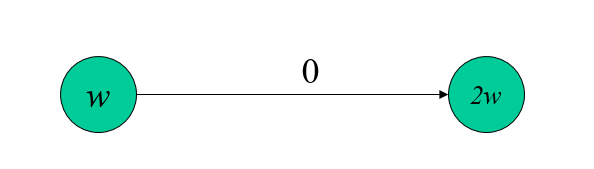
\includegraphics[width=0.5\textwidth]{figures/L8-2states.png}\\
  \caption{Two state snippet of an MDP }\label{fig:L8-2state}
  \end{centering}
\end{figure}

Consider the following part of an MDP (see Figure
\ref{fig:L8-2state}) consists of two nodes, with a transition from
the first to the second, with reward $0$. The main issue is that the
linear approximation gives the first node a weight $\weight$ and the
second $2\weight$. Assume we start with some value $\weight_0>0$.
Each time we have an update for the two states we have
\[
\weight_{\ttime+1}=\weight_\ttime +\alpha[0+\gamma
(2\weight_\ttime)-\weight_\ttime]=[1+\alpha(2\gamma-1)]\weight_\ttime=[1+\alpha(2\gamma-1)]^\ttime\weight_1
\]
For $\gamma>0.5$ we have $\alpha(2\gamma-1)>0$, and $\weight_\ttime$
diverges.

We are implicitly assuming that the setting is off-policy, since in
an on-policy, we would continue from the second state, and
eventually lower the weight.

To have a ``complete'' example consider the three state MDP in
Figure~\ref{fig:L8-3state}. All the rewards are zero, and the main
difference is that we have a new terminating state, that we reach
with probability $p$.

\begin{figure}
  % Requires \usepackage{graphicx}
  \begin{centering}
  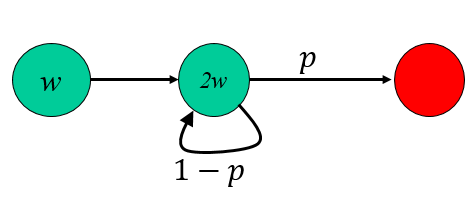
\includegraphics[width=0.5\textwidth]{figures/L8-3state.png}\\
  \caption{The three state MDP. All rewards are zero.}\label{fig:L8-3state}
  \end{centering}
\end{figure}




Again, assume that we start with some $\weight_0>0$ We have three
types of updates, one per possible transition. When we transition
from the initial state to the second state we have
\[
\Delta \weight= \alpha[0+\gamma
(2\weight_\ttime)-\weight_\ttime]\cdot
1=\alpha(2\gamma-1)\weight_\ttime
\]
The transition from the second state back to itself has an update,
\[
\Delta \weight= \alpha[0+\gamma
(2\weight_\ttime)-(2\weight_\ttime)]\cdot 2
=-4\alpha(1-\gamma)\weight_\ttime
\]
The transition to the terminal state we have
\[
\Delta \weight= \alpha[0+\gamma 0 -(2\weight_\ttime)]\cdot
2=-4\alpha \weight_\ttime
\]



When we use on-policy, we have all transitions. Assume that the
second transition happens $n\geq 0$ times. Then we have
\[
\frac{\weight_{\ttime+1}}{\weight_\ttime}=(1+\alpha(2\gamma-1))(1-4\alpha(1-\gamma))^n(1-4\alpha)<
1-\alpha
\]
This implies that $\weight_\ttime$ converges to zero, as desired.

Now consider an off-policy that truncates the episodes after $n$
transitions of the second state, where $n\ll 1/p$, and in addition
$\gamma> 1-1/(40n)$. This implies that in most updates we do not
reach the terminal state and we have
\[
\frac{\weight_{\ttime+1}}{\weight_\ttime}=(1+\alpha(2\gamma-1))(1-4\alpha(1-\gamma))^n>1
\]
and therefore, for the some setting of $n$ we have that the weight
$\weight_\ttime$ diverges.

We might hope that the divergence is due to the online nature of the
TD updates. We can consider an algorithm that in each iteration
minimizes the square error. Namely,
\[
\weight_{\ttime+1}=\arg\min_\weight\sum_s
[\widehat{V}(\state_\ttime;\weight)-E^\policy[\reward_\ttime+\gamma\widehat{V}(\state_{\ttime+1};\weight_\ttime)]]^2
\]

For the MDP example of Figure~\ref{fig:L8-3state} we have that:
\begin{align*}
 \weight_{\ttime+1} &= \arg\min_\weight (\weight-\gamma(2\weight_\ttime))^2+(2\weight-(1-p)\gamma(2\weight_\ttime))^2
\end{align*}
Solving for $\weight_{\ttime+1}$ we have
\begin{align*}
0&=  2(\weight_{\ttime+1}-\gamma(2\weight_\ttime))+4(2\weight_{\ttime+1}-(1-p)\gamma(2\weight_\ttime)\\
  10 \weight_{\ttime+1}&=4\gamma \weight_\ttime + 8\gamma(1-p)\weight_\ttime\\
  \weight_{\ttime+1}&=\frac{6-4p}{5}\gamma \weight_\ttime
\end{align*}
So for $\gamma(6-4p)>5$ we have divergence. (Recall that
$\gamma\approx 1-\varepsilon$ and $p\approx \varepsilon$ is a very
important setting.)

Note that if we have taken in to account the influence of
$\weight_{\ttime+1}$ on $V$ and use
$\widehat{V}(\state_{\ttime+1};\weight_{\ttime+1})$ instead of
$\widehat{V}(\state_{\ttime+1};\weight_\ttime)$, this specific
problem would have disappeared, since $\weight_{\ttime+1}=0$ would
be the minimizer.

\section{Summary}

What we have seen, as Rich Sutton says, that there is a {\em deadly
triad}:
\begin{enumerate}
\item
Function Approximation
\item
Bootstrapping methods, such as TD.
\item
Off-policy training.
\end{enumerate}
When the three conditions hold, many times we have counter examples for the convergence.

Here is a summary of the known convergence and divergence results in
the literature:
\begin{center}
  \begin{tabular}{ | l | c | c|c|c| }
    \hline
    & algorithm & look-up table&linear function&non-linear\\ \hline
    on-policy & MC & + & + & + \\ \hline
    on-policy & $TD(0),TD(\lambda)$ & + & + & -\\ \hline
 %   on-policy & $TD(\lambda)$ & + & + & - \\ \hline
    off-policy & MC & + & + & + \\ \hline
    off-policy & $TD(0),TD(\lambda)$ & + & - & -\\ \hline
 %   off-policy & $TD(\lambda)$ & + & - & - \\ \hline
  \end{tabular}
\end{center}

The results for the look-up table where derived in Chapter
\ref{chapter:learning-model-free}.
%
The fact that Monte-Carlo methods converge is due to the fact that
they are running an SGD algorithm. For linear functions with convex
loss they will converge to the global optimum and for non-linear
functions (for example, neural networks) they will converge to a
local optima. The convergence to the TD appear in Chapter
\ref{sec:FA-Advanced}. The divergence of TD with linear fucntions in
an off-policy setting appear in Chapter \ref{sec:TD-FA}. The TD
divergence in the non-linear online setting appears in
\cite{TsitsiklisVR97}.


%\newpage
\begin{leftbar}
\section{Advanced topics}
\label{sec:FA-Advanced}

\subsection{Comparing $\weight_{min}$ and $\weight_{TD}$}

The derivation follows \cite{TsitsiklisVR97}, however, for
simplicity, we limit ourselves to $TD(0)$ rather than $TD(\lambda)$.

We will need to start with a few definitions. Given the steady state
distribution $\mu(\state)$ for $\state\in \States$ we define a
diagonal matrix $D$ of size $|\States|\times|\States|$ where
$D(\state,\state)=\mu(\state)$. We define an inner-product
$\langle\cdot,\cdot\rangle_D$ where $\langle
z_1,z_2\rangle_D=z_1^\top Dz_2$ and a norm $\|z\|_D=\sqrt{<z,z>_D}$.

We define $\operator^\policy(V)= \reward + \gamma PV$ and recall
that: (1) $\Value^\policy = \operator^\policy(\Value^\policy)$, (2)
$\|\operator^\policy(V_1)-\operator^\policy(V_2)\|_D\leq \gamma
\|V_1-V_2\|_D$ (actually we we need to prove that for
$\|\cdot\|_D$).

We will perform a linear function approximation where the attributes
of state $\state$ are $x_\state$. Define a matrix $X$ of size
$|\States|\times d$, where the $\state$ row is $x_\state$. Then
using a parameter $\weight$ our approximation is
$\widehat{V}(\cdot;\weight)=X\weight$. We now need to project
vectors to an approximation $X\weight$. Give a vector $V$, let
$\Pi(V)=\arg\min_\weight \|X\weight-V\|_D$. This projection
operation can be written explicitly as
\[
\Pi(V)=X(X^\top DX)^{-1}X^\top D V.
\]


We can write the expected update as:
\[
\Delta \weight= X^\top D(T^\policy(X\weight_\ttime)-X\weight)
\]
which is the gradient of
\[
\nabla_\weight \|T^\policy(X\weight_\ttime)-Xw\|_D^2
\]
note that the input to $T^\policy$ is fixed and we optimize over
$\weight$ only. The minimization is
\[
\weight_{\ttime+1}=\Pi(T^\policy(X\weight_\ttime))
\]

We will need the following technical claim:
\begin{claim}
\[
\|PV\|_D^2\leq \|V\|_D^2
\]
\end{claim}

\begin{proof}
\begin{align*}
\|PV\|_D^2 & =V^\top P^\top D P V \\
&= \sum_s \mu(\state) (\sum_{\state'} p(\state'|\state) V(\state'))^2\\
&\leq \sum_s \mu(\state) \sum_{\state'} p(\state'|\state) V^2(\state')\\
&=\sum_{\state'} V^2(\state') \sum_s \mu(\state)p(\state'|\state)\\
&=\sum_{\state'} \mu(\state')V^2(\state')=\|V\|_D
\end{align*}
\end{proof}

\begin{lemma}
Let $\weight_{TD}$ be the limit of
$\weight_{\ttime+1}=\Pi(T^\policy(X\weight_\ttime))$, i.e., using
$TD(0)$. Then,
\[
\|X\weight_{TD}-\Value^\policy\|_D\leq
\frac{1}{1-\gamma}\|X\weight_{min}-\Value^\policy\|_D
\]
\end{lemma}

\begin{proof}
By definition, $\weight_{min}$ is the projection of $\Value^\policy$
to $X$, i.e., $\Pi(\Value^\policy)$. Note that we have
$\Value^\policy=
\Pi(\Value^\policy)+(\Value^\policy-\Pi(\Value^\policy))$ and
$\langle\Pi(\Value^\policy),\Value^\policy-\Pi(\Value^\policy)\rangle_D=0$,
otherwise we can improve. This implies that
$\|\Value^\policy\|_D=\|\Pi(\Value^\policy)\|_D+\|\Value^\policy-\Pi(\Value^\policy)\|_D$.
\begin{align*}
\|X\weight_{TD}-\Value^\policy\| &\leq
\|X\weight_{TD}-\Pi(\Value^\policy\|_D+\|\Pi(\Value^\policy)-\Value^\policy\|_D\\
&= \|\Pi(T^\policy(X\weight_{TD}))-\Pi(\Value^\policy)\|_D+\|\Pi(\Value^\policy)-\Value^\policy\|_D\\
&\leq \|T^\policy(X\weight_{TD})-\Value^\policy\|_D+\|\Pi(\Value^\policy)-\Value^\policy\|_D\\
&\leq \gamma \|X\weight_{TD}-\Value^\policy\|_D+\|\Pi(\Value^\policy)-\Value^\policy\|_D\\
\end{align*}
and the lemma follows since $\Pi(\Value^\policy)=X\weight_{min}$ by
definition of $\weight_{min}$.
\end{proof}


\subsection{LSTD}


We consider least Squares Temporal Difference (LSTD). We will
analyze $LSTD(0)$.

Let $x_\ttime=x_{\state_\ttime}$. The weights:
\begin{align*}
\weight_{\ttime+1} &= \weight_\ttime +\alpha (\reward_\ttime+\gamma
\weight_\ttime^\top x_{\ttime+1}-\weight_\ttime^\top
x_\ttime)x_\ttime\\
\weight_{\ttime+1} &= \weight_\ttime +\alpha (\reward_\ttime
x_\ttime-x_\ttime(x_\ttime-\gamma x_{\ttime+1})^\top \weight_\ttime)
\end{align*}

We have that
\[
E[\weight_{\ttime+1}|\weight_\ttime]=\weight_\ttime +\alpha
(b-A\weight_\ttime)
\]
where $b=E[\reward_\ttime x_\ttime]\in \Reals^d$ and
$A=E[x_\ttime(x_\ttime-\gamma x_{\ttime+1})^\top]\in\Reals^{d\times
d}$.

At convergence we have $\weight=A^{-1}b$.

\end{leftbar}


\section{Applications: games}

\subsection{Backgammon}

Tesauro developed the TD-gammon in the late 1980's and 1990's. The
system uses a neural network approximation, using a $TD(\lambda)$
updates. The initial system was able to win against other computer
programs, which where hand-designed, and later matched the
performance of the best human. For the training the system used
self-play, namely playing against itself.

The neural network has a single hidden layer (with $40/80/160$
nodes, in the three different generations of the project). There are
$198$ inputs. The hidden layer has sigmoidal nodes with
$\sigma(z)=\frac{1}{1+e^{-z}}$. The output $y$ can be viewed as the
probability of winning from a given position.

The $198$ inputs are composed as follows. For each of the $24$ slots
and for each of the two colors, we have four Boolean inputs. The
first indicates if there is a single chip, the second indicates two
or more chips, the third indicates exactly three chips and the
fourth indicates four or more chips. We have two Boolean variables
that indicate who turn it is (one for white and one for black).
Finally, we have two aggregate inputs, per color: (1) number of
chips divided by $2$ and (2) number of chips removed divided by
$15$.

The TD-gammon uses the standard TD updates.
\[
\Delta \weight_\ttime =
\alpha(y_\ttime-y_{\ttime-1})\sum_{k=1}^{t}\lambda^{\ttime-k}\nabla_\weight
y_k
\]
When the game ends we replace $y_\ttime$ by $z$ the outcome of the
game.



The evaluation of the position is done using a max-min tree, whose
depth is $1/2/3$ (depending on the generation). The max-min tree has max layer where the value of
a node is the maximum of their children, and min layer, where the
value of a node is the minimum of their children. Given the tree (of
size at most $20/400/8000$ in different generations) we evaluate the
leaves using the neural network, and propagate the values in the
min-max tree to get the predicted value of a position.

The network is initialized with small random weights. Note that due
to the game nature, even with random policies the game terminates.
The training is done using self-play, where the number of games was
$300K/800K/1500K$ in different generations.

One very intriguing aspect  of the TD-gammon is that it {\em
improved the human performance}. For example, when the first role is
{\tt 4-1}, grandmasters did the $1$ move in location $6$, while the
TD-gammon moved location $24$. Following the TD-gammon, grandmasters
changed their view and started playing those positions in the same
way that TD-gammon did.

\subsection{Attari games}

The system was developed by DeepMind researchers during $2013-2015$.
The system learns to play from the raw video frames, a variety of
$49$ games. The learning uses a neural network and employs
$Q$-learning (and a Deep-Q-Network, DQN).

The neural network works as follows. There is a preprocessing stage
that maps frames of size $210\times 160$ with 128-colors, to
$84\times 84$ and 4-colors. This mapping is fixed and shared by all
games. The neural network has three convolutional layers followed by
one completely connected layer. The output layer has multiple
outputs. The nodes in the network use RelU gates.

The DQN innovations are: (1) Experience reply, reusing the same
example many times, (2) fixed Q-target, when setting the target
update, and (3) clipping the error. To better understand the
innovations, we need to consider the flow of the training.

In the training, we first select an action $\action_\ttime$, using
$\varepsilon$-greedy policy. We observe the reward and the next
state
$(\state_\ttime,\action_\ttime,\reward_\ttime,\state_{\ttime+1})$,
and store them in the reply memory. We sample a mini-batch from the
reply memory. For each sample we use the fixed-Q-target (more
latter). We use the SGD to minimize the MSE.

For the fixed-Q-target, we do the update as follows. We have two
sets of weights $\weight_\ttime$, the current weights, and
$\weight^-_\ttime$ as the fixed weights. We update $\weight_\ttime$
to $\weight^-_\ttime$ every (large) number of plays, setting
$\weight_\ttime=\weight^-_\ttime$. The update at time $\ttime$
becomes:
\[
\Delta \weight_\ttime = \alpha \Gamma_\ttime \nabla_{\weight_\ttime}
Q(\state_\ttime,\action_\ttime;\weight_\ttime)
\]
where
\[
\Gamma_{\ttime}=\reward_\ttime+\gamma \max_\action
Q(\state_{\ttime+1},\action;\weight^-_\ttime)-Q(\state_\ttime,\action_\ttime;\weight_\ttime)
\]
Note that $\weight^-_\ttime$ is used only to estimate the future
return from $\state_{\ttime+1}$. The clipping enforces
$\Gamma_\ttime\in[-1,+1]$.

The system is able to match human performance in $29$ out of $49$
Attari games.







\section{Bibliography Remarks}

The work of Gerald Tesauro on TD-gammon is described in
\cite{Tesauro95,Tesauro02}.

The DeepMind system for playing Attari games is described in
\cite{MnihKSRVBGRFOPB15}.


Part of the outline borrows from David Silver class notes and the
the book of Sutton and Barto \cite{SuttonB98}.

% %%\newpage
\begin{leftbar}
\section{Advanced topics}
\label{sec:FA-Advanced}

\subsection{Comparing $\weight_{min}$ and $\weight_{TD}$}

The derivation follows \cite{TsitsiklisVR97}, however we limit
ourselves to $TD(0)$ rather than $TD(\lambda)$.

We will need to start with a few definitions. Given the steady state
distribution $\mu(\state)$ for $s\in S$ we define a diagonal matrix
$D$ of size $|S|\times|S|$ where $D(\state,\state)=\mu(\state)$. We
define an inner-product $<\cdot,\cdot>_D$ where
$<z_1,z_2>_D=z_1^\top Dz_2$ and a norm $\|z\|_D=\sqrt{<z,z>_D}$.

We define $T^\policy(V)= r + \gamma PV$ and recall that: (1)
$\Value^\policy = T^\policy(\Value^\policy)$, (2)
$\|T^\policy(V_1)-T^\policy(V_2)\|_d\leq \gamma \|V_1-V_2\|_D$
(actually we we need to prove that for $\|\cdot\|_D$).

We will perform a linear function approximation where the attributes
of state $\state$ are $x_s$. Define a matrix $X$ of size $|S|\times
d$, where the $\state$ row is $x_s$. Then using a parameter
$\weight$ our approximation is $\widehat{V}(\cdot;\weight)=Xw$. We
now need to project vectors to an approximation $Xw$. Give a vector
$V$, let $\Pi(V)=\arg\min_\weight \|Xw-V\|_D$. This projection
operation can be written explicitly as
\[
\Pi(V)=X(X^\top DX)^{-1}X^\top D V.
\]


We can write the expected update as:
\[
\Delta w= X^\top D(T^\policy(X\weight_\ttime)-Xw)
\]
which is the gradient of
\[
\nabla_\weight \|T^\policy(X\weight_\ttime)-Xw\|_D^2
\]
note that the input to $T^\policy$ is fixed and we optimize over
$\weight$ only. The minimization is
\[
\weight_{\ttime+1}=\Pi(T^\policy(X\weight_\ttime))
\]

We will need the following technical claim:
\begin{claim}
\[
\|PV\|_D^2\leq \|V\|_D^2
\]
\end{claim}

\begin{proof}
\begin{align*}
\|PV\|_D^2 & =\Value^\top P^\top D P V \\
&= \sum_s \mu(\state) (\sum_{\state'} p(\state'|\state) V(\state'))^2\\
&=\sum_s \mu(\state) \sum_{\state'} p(\state'|\state) \Value^2(\state')\\
&=\sum_{\state'} \Value^2(\state') \sum_s \mu(\state)p(\state'|\state)\\
&=\sum_{\state'} \mu(\state')\Value^2(\state')=\|V\|_D
\end{align*}
\end{proof}

\begin{lemma}
Let $\weight_{TD}$ be the limit of
$\weight_{\ttime+1}=\Pi(T^\policy(X\weight_\ttime))$, i.e., using
$TD(0)$. Then,
\[
\|X\weight_{TD}-\Value^\policy\|_D\leq
\frac{1}{1-\gamma}\|X\weight_{min}-\Value^\policy\|_D
\]
\end{lemma}

\begin{proof}
By definition, $\weight_{min}$ is the projection of $\Value^\policy$
to $X$, i.e., $\Pi(\Value^\policy)$. Note that we have
$\Value^\policy=
\Pi(\Value^\policy)+(\Value^\policy-\Pi(\Value^\policy))$ and
$<\Pi(\Value^\policy),\Value^\policy-\Pi(\Value^\policy)>_D=0$,
otherwise we can improve. This implies that
$\|\Value^\policy\|_D=\|\Pi(\Value^\policy)\|_D+\|\Value^\policy-\Pi(\Value^\policy)\|_D$.
\begin{align*}
\|X\weight_{TD}-\Value^\policy\| &\leq
\|X\weight_{TD}-\Pi(\Value^\policy\|_D+\|\Pi(\Value^\policy)-\Value^\policy\|_D\\
&= \|\Pi(T^\policy(X\weight_{TD}))-\Pi(\Value^\policy)\|_D+\|\Pi(\Value^\policy)-\Value^\policy\|_D\\
&\leq \|T^\policy(X\weight_{TD})-\Value^\policy\|_D+\|\Pi(\Value^\policy)-\Value^\policy\|_D\\
&\leq \gamma \|X\weight_{TD}-\Value^\policy\|_D+\|\Pi(\Value^\policy)-\Value^\policy\|_D\\
\end{align*}
and the lemma follows since $\Pi(\Value^\policy)=X\weight_{min}$ be
definition of $\weight_{min}$.
\end{proof}


\section{LSTD}


We consider least Squares Temporal Difference (LSTD). We will
analyze $LSTD(0)$.

Let $x_\ttime=x_{\state_\ttime}$. The weights:
\begin{align*}
\weight_{\ttime+1} &= \weight_\ttime +\alpha (\reward_\ttime+\gamma
\weight_\ttime^\top x_{\ttime+1}-\weight_\ttime^\top
x_\ttime)x_\ttime\\
\weight_{\ttime+1} &= \weight_\ttime +\alpha (\reward_\ttime
x_\ttime-x_\ttime(x_\ttime-\gamma x_{\ttime+1})^\top \weight_\ttime)
\end{align*}

We have that
\[
E[\weight_{\ttime+1}|\weight_\ttime]=\weight_\ttime +\alpha
(b-A\weight_\ttime)
\]
where $b=E[\reward_\ttime x_\ttime]\in \Reals^d$ and
$A=E[x_\ttime(x_\ttime-\gamma x_{\ttime+1})^\top]\in\Reals^{d\times
d}$.

At convergence we have $\weight=A^{-1}b$.

\end{leftbar}

% %\input{exercises8}

% \chapter{Large state space: Policy Gradient Methods}
% This chapter continues looking at the case where the MDP models are
large state space. In the previous chapter we looked at
approximating the value function. In this chapter we will consider
learning directly a policy and optimizing it.

The main advantages and disadvantages of policy optimization (rather
than value function approximation) are the following:
\begin{enumerate}
\item
Continuous action space. In such a case the policy optimization
method is the most natural and the one which is used in practice
(for applications such as robotics).
\item
Convergence: While the policy optimization would normally converge,
it will most likely converge to a local optimum.
\item
High dimensional spaces: It can be fairly effective in selecting the
actions (in contrast to learning accurate values).
\item
Evaluation time would typically be longer (compared to value
function approaches).
\item
Stochastic Policy: allows naturally to have a stochastic policy.
\end{enumerate}

\section{Stochastic policies}

We have seen that the optimal policy in an MDP is deterministic, so
what benefit can be in considering a stochastic policy?

The main benefit is in situations where there is a
miss-specification of the model. The main issue is that the state
encoding might create a system which is not Markovian anymore, by
coalescing certain states which have identical encoding. We will
give two example of this phenomena.

\paragraph{Aliased Grid-world}\ \\
Consider the example in Figure~\ref{fig:L9-grid-world}. The green
state is the good goal and the red ones are the bad. The encoding of
each state is the location of the walls. In each state we need to
choose a direction. The problem is that we have two states which are
indistinguishable (marked by question mark).

It is not hard to see that any deterministic policy would fail from
some start state (either the left or the right one). Alternatively,
we can use a randomized policy in those states,with probability half
go right and probability half go left. For such a policy we have a
rather short time to reach the green goal state (and avoid the red
states).

The issue here was that two different states had the same encoding,
and thus violated the Markovian assumption. This can occur when we
encode the state with a small set of features, and some (hopefully,
similar) states coallesce to a single representation.

\begin{figure}
  % Requires \usepackage{graphicx}
  \begin{centering}
  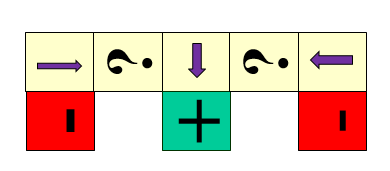
\includegraphics[width=0.5\textwidth]{figures/L9-grid-world.png}\\
  \caption{Grid-world example }\label{fig:L9-grid-world}
  \end{centering}
\end{figure}

\paragraph{Zero-sum games}\ \\
The MDP model was not design for interactive zero-sum games,
however, in many of the applications we saw, we train a policy to
play a board game (such as backgammon). Any board game is an
instance of a zero-sum game, since if one player wins the other
loses. In alternating-moves games, the optimal policy would still be
deterministic, but this is not the case in simultaneous-move games.

%The main issue with a more general game, is the the optimal policy
%might be stochastic.

Consider a penny-matching game, in which each player simultaneously
select a bit $\{0,1\}$. If the two selected bits are identical the
first player wins and if they differ the second player wins. The
best policy for each player is stochastic (selecting each bit with
probability half).

An important observation is that if one of the player plays
deterministically (or almost deterministically), then the other
player can win (or almost always win) by selecting
(deterministically) the appropriate action. For this reason, even
any $\varepsilon$-greedy would have a poor performance.

Here we violated the assumption that the rewards depend only on the
state. In this example they depend indirectly on the policy
selected.

\section{Policy optimization}

We will assume that each state $\state$ has an encoding
$\phi(\state)\in \mathbb{R}^{d_1}$. The policy will have a
parametrization $\theta\in \mathbb{R}^{d_2}$. The policy will be
based on the two encodings, and we have
$\policy(\action|\state,\theta)$, which is the probability of
selecting action $\action$ when observing state $\state$ (or,
equivalently, $\phi(\state)$), and having a policy parametrization
$\theta$.

The optimization problem would be:
\[
\theta^* = \arg\max_\theta J(\theta)
\]
where $J(\theta) \triangleq \Value^\policy(\state_0)$ is the
expected return of the policy $\policy(\cdot|\cdot,\theta)$ from the
initial state $\state_0$.
%
This maximization problem can be solved in multiple ways. We will
mainly explore gradient based methods.

We start by giving a few examples on how to parameterize the policy.
The first is a {\em log linear policy}. We will assume an encoding
of the state and action pairs, i.e., $\phi(\state,\action)$. The
linear part will compute
$\mu(\state,\action)=\phi(\state,\action)^\top \theta$. Given the
values of $\mu(\state,\action)$ for each $\action\in \Actions$, the
policy select action $\action$ with probability proportional to
$e^{\mu(\state,\action)}$. Namely,
\[
\policy(\action|\state,\theta)=
\frac{e^{\mu(\state,\action)}}{\sum_{b\in
\Actions}e^{\mu(\state,b)}}
\]

The second example is a {\em Gaussian policy}, where the action
space is a real number, i.e., $A=\mathbb{R}$. The encoding is of
states, and the actions are any real number. Given a state $\state$
we compute $\mu(\state)=\phi(\state)^\top\theta$. We select an
action $\action$ from the normal distribution with mean
$\mu(\state)$ and variance $\sigma^2$, i.e.,
$N(\mu(\state),\sigma^2)$. (The Gaussian policy has an additional
parameter $\sigma$.)

We would like to use the policy gradient to optimize the expected
return  $J(\theta)$ of the policy $\policy(\cdot|\cdot,\theta)$. We
will compute the gradient of $J(\theta)$, i.e., $\nabla_\theta
J(\theta)$. The update of the policy parameter $\theta$ is
\[
\theta_{\ttime+1}=\theta_\ttime + \alpha \nabla_{\theta_\ttime}
J(\theta_\ttime)
\]
where $\alpha$ is a learning rate.

One challenge we will have to address is to relate $\nabla_\theta
J(\theta)$ to the gradients $\nabla \policy(\action|\state,\theta)$.

\subsection{Finite differences methods}

This methods can be used even when we do not have a representation
of the gradient of the policy or even the policy itself. This may
arise many times when we have, for example, access to an
off-the-shelf robot for which the software is encoded already in the
robot. In such cases we can estimate the gradient by introducing
perturbations in the parameters.

The simplest case is component-wise gradient estimates. Let $e_i$ be
a unit vector, i.e., has in the $i$-th entry a value $1$ and a value
$0$ in all the other entries. The perturbation that we will add is
$\delta e_i$ for some $\delta >0$. We will use the following
approximation:
\[
\frac{\partial}{\partial \theta_i}J(\theta)\approx
\frac{\hat{J}(\theta+\delta e_i)-\hat{J}(\theta)}{\delta}
\]
where $\hat{J}(\theta)$ is unbiased estimator of $J(\theta)$. A more
symmetric approximation is sometimes better,
\[
\frac{\partial}{\partial \theta_i}J(\theta)\approx
\frac{\hat{J}(\theta+\delta e_i)-\hat{J}(\theta-\delta e_i
)}{2\delta}
\]

The problem is that we need to average many samples of
$\hat{J}(\theta\pm\delta e_i)$ to overcome the noise. Another
weakness is that we need to do the computation per dimension. In
addition, the selection of $\delta$ is also critical. A small
$\delta$ might have a large noise rate that we need to overcome (by
using many samples). A large $\delta$ run the risk of facing the
non-linearity of $J$.

Rather then doing the computation per dimension, we can do a more
global approach and use a least squares estimation of the gradient.
Consider a random vector $u_i$, then we have
\[
J(\theta+\delta u_i)\approx J(\theta)+\delta (u_i)^\top \nabla
J(\theta)
\]
We can define the following least square problem,
\[
G= \arg\min_x \sum_i (J(\theta+\delta u_i)- J(\theta)-\delta
(u_i)^\top x)^2,
\]
where $G$ is our estimate for $\nabla J(\theta)$.

We can move to matrix notation and define $\Delta
J^{(i)}=J(\theta+\delta u_i)- J(\theta)$ and $\Delta J= [\cdots ,
\Delta J^{(i)}, \cdots]^\top$. We define $\Delta \theta^{(i)}=\delta
u_i$, and the matrix $[\Delta\Theta]=[\cdots
\Delta\theta^{(i)},\cdots]^\top$, where the $i$-th row is
$\Delta\theta^{(i)}$.

We would like to solve for the gradient, i.e,
\[
\Delta J\approx [\Delta \Theta]x
\]
This is a standard least square problem and the solution is
\[
G=([\Delta \Theta]^\top [\Delta \Theta])^{-1} [\Delta\Theta]^\top
\Delta J
\]

One issue that we neglected is that we actually do not a have the
value of $J(\theta)$. The solution is to solve also for the value of
$J(\theta)$.
%
We can define a matrix $M=[1, [\Delta\Theta]]$, a vector of unknowns
$x=[J(\theta), \nabla J(\theta)]$, and have the target be
$z=[\cdots, J(\theta+\delta u_i),\cdots]$. We can now solve for
$z\approx Mx$, and this will recover an estimate also for
$J(\theta)$.


\section{Policy Gradient Theorem}

The policy gradient theorem will relate the gradient of the expected
return $\nabla J(\theta)$ and the gradients of the policy $\nabla
\policy(\action|\state,\theta)$. We will mainly try to make sure
that we are able to use it to get estimates, and the quantities
would be indeed observable by the learner.

We will state the policy gradient theorem for the finite-horizon
return, but it also holds for the discounted return and average
reward return. Recall that the finite-horizon return is
$\sum_{\ttime=1}^\tHorizon \reward_\ttime$ and
$\Value^\policy(\state)=E[\sum_{\ttime=1}^\tHorizon
\reward_\ttime|\state_1=\state]$.

\begin{theorem}[Policy Gradient Theorem]
\label{thm:policy-gradient} For any policy
$\policy(\cdot|\cdot;\theta)$, we have
\[
\nabla J(\theta)\propto \sum_{s\in S} \mu(\state) \sum_{\action\in
\Actions} Q^\policy (\state,\action)\nabla_\theta
\policy(\action|\state;\theta)
\]
where $\mu(\state)=\nu(\state)/\tHorizon$ and
$\nu(\state)=\sum_{\ttime=1}^\tHorizon\Pr[\state_\ttime=\state|\state_1,\theta]$.
\end{theorem}

\begin{proof}
For each state $\state$ we have
\begin{align*}
\nabla \Value^\policy(\state) &= \nabla \sum_\action \policy(\action|\state) Q^\policy(\state,\action)\\
&=\sum_\action  Q^\policy(\state,\action) \nabla \policy(\action|\state) + \policy(\action|\state) \nabla Q^\policy(\state,\action)\\
&=\sum_\action  Q^\policy(\state,\action) \nabla \policy(\action|\state) + \policy(\action|\state) \sum_{\state_1} p(\state_1|\state,\action) \nabla \Value^\policy(\state_1)\\
&= \sum_\action  Q^\policy(\state,\action) \nabla
\policy(\action|\state) + \sum_{\state_1} p(\state_1|\state)
\nabla \Value^\policy(\state_1)\\
&= \sum_\action  Q^\policy(\state,\action) \nabla
\policy(\action|\state) + \sum_{\state_1} p(\state_1|\state)
\sum_\action Q^\policy(\state_1,\action) \nabla
\policy(\action|\state_1) + \sum_{\state_2}
p(\state_2|\state_1)p(\state_1|\state)
\nabla \Value^\policy(\state_2)\\
& = \sum_{x\in
S}\sum_{\ttime=1}^\tHorizon\Pr[\state_\ttime=x|\state_1=\state,\policy]\sum_\action
Q^\policy (x,\action)\nabla\policy(\action|x)
\end{align*}
where the first identity follows since by averaging
$Q^\policy(\state,\action)$ over the actions $\action$ with the
probabilities induce by $\policy(\action|\state)$ we have right
expectation of the immediate reward. The next state is distributed
correctly, and therefore the identity holds. The second equality
follows from the gradient of a multiplication. The third follows
since $\nabla Q^\policy(\state,\action)= \nabla
[\reward(\state,\action)+\gamma
\sum_{\state'}p(\state'|\state,\action)\Value^\policy(\state'|\state,\action)]$.
%
The next two identities role the policy one step in to the future.
%
The last identity follows from unrolling $\state'$ to $\state''$,
etc. and then reorganizing the terms.

Using this we have
\begin{align*}
\nabla J(\theta) &= \nabla \Value^\policy (\state_0)\\
&= \sum_\state \left(\sum_{\ttime=1}^\tHorizon\Pr[\state_\ttime=\state|\state_0,\policy] \right) \sum_\action Q^\policy (\state,\action) \nabla\policy(\action|\state) \\
&= \sum_\state \nu(\state) \sum_\action Q^\policy (\state,\action) \nabla\policy(\action|\state) \\
%&= \left(\sum_s \eta(\state)\right)\sum_s \frac{\eta(\state)}{\sum_x \eta(x)}  \sum_\action\nabla\policy(\action|\state) Q^\policy (\state,\action) \\
&= \tHorizon  \sum_s \mu(\state) \sum_\action Q^\policy
(\state,\action) \nabla\policy(\action|\state)
\end{align*}
\end{proof}

\begin{example}
Consider an MDP with a single state $\state$ (which is also called
Multi-Arm Bandit, and is discussed in Chapter \ref{chapter:MAB}).
Assume we have only two actions, action $\action_1$ has expected
reward $\reward_1$ and action $\action_2$ has expected reward
$\reward_2$.

The policy $\policy$ is define with a parameter
$\theta=(\theta_1,\theta_2)$, where $\theta_i\in \reals$. Given
$\theta$ the probability of action $\action_i$ is
$p_i=e^{\theta_i}/(e^{\theta_1}+e^{\theta_2})$. We will also select
a horizon of length one, i..e, $\tHorizon=1$. This implies that
$Q^\policy(\state,\action_i)=\reward_i$.

In this simple case we can compute directly $J(\theta)$ and $\nabla
J(\theta)$. The expected return is simply,
\[
J(\theta)=p_1 \reward_1 + p_2 \reward_2 =
\frac{e^{\theta_1}}{e^{\theta_1}+e^{\theta_2}} \reward_1 +
\frac{e^{\theta_2}}{e^{\theta_1}+e^{\theta_2}} \reward_2
\]
Note that $\frac{\partial}{\partial \theta_1} p_1=
p_1-p_1^2=p_1(1-p_1) $ and $\frac{\partial }{\partial \theta_2} p_1=
- p_1 p_2= -p_1(1-p_1)$. The gradient is
\[
\nabla J(\theta)= \reward_1 \begin{pmatrix} p_1(1-p_1)\\
-p_1(1-p_1)\end{pmatrix} + \reward_2 \begin{pmatrix} -p_1(1-p_1)\\
p_1(1-p_1)\end{pmatrix} = (\reward_1-\reward_2) p_1(1-p_1) \begin{pmatrix}+1\\
-1\end{pmatrix}
\]
Updating in the direction of the gradient, in the case that
$\reward_1>\reward_2$, would increase $\theta_1$ and decrease
$\theta_2$, which will imply that $p_1$ will converge to $1$.

To apply the Policy gradient theorem we need to compute the
gradient,
\[
\nabla_\theta \policy(\action_1|\state;\theta) = \nabla \begin{pmatrix} p_1\\
1-p_1\end{pmatrix}=  \begin{pmatrix} p_1(1-p_1)\\
-p_1(1-p_1)\end{pmatrix}
\]
and the policy gradient theorem gives us the same expression,
\[
\nabla J(\theta) \propto \reward_1 \nabla
\policy(\action_1|\theta)+\reward_2 \nabla
\policy(\action_2|\theta)=\reward_1 \begin{pmatrix} p_1(1-p_1)\\
-p_1(1-p_1)\end{pmatrix} + \reward_2 \begin{pmatrix} -p_1(1-p_1)\\
p_1(1-p_1)\end{pmatrix}
\]
where we used the fact that there is only a single state $\state$,
and that $Q^\policy(\state,\action_i)=\reward_i$.
\end{example}

The Policy Gradient Theorem gives us a way to compute the gradient.
We can sample states from the distribution $\mu(\state)$ using the
policy $\policy$. We still need to resolve the sampling of the
action. We are going to observe the outcome of only one action in
state $\state$, and the theorem requires summing over all of them!
In the following we will slightly modify the theorem so that we will
be able to use only the action $\action$ selected by the policy
$\policy$, rather than summing over all actions.

Consider the following simple identity,
\[
\nabla f(x)=f(x)\frac{\nabla f(x)}{f(x)}=f(x)\nabla \log f(x)
\]
This implies that we can restate the Policy Gradient Theorem as the
following corollary,
\begin{corollary}[Policy Gradient Corollary]
\label{thm:policy-gradient} For any policy
$\policy(\cdot|\cdot;\theta)$, we have
\[
\nabla J(\theta)\propto \sum_{s\in S} \mu(\state) \sum_{\action\in
\Actions} \policy(\action|\state;\theta) Q^\policy
(\state,\action)\nabla_\theta \log \policy(\action|\state;\theta) =
E^\policy[Q^\policy (\state,\action)\nabla_\theta \log
\policy(\action|\state;\theta)]
\]
where $\mu(\state)=\nu(\state)/\tHorizon$ and
$\nu(\state)=\sum_{\ttime=1}^\tHorizon\Pr[\state_\ttime=\state|\state_1,\theta]$.
\end{corollary}
Note that in the above corollary both the state $\state$ and action
$\action$ are sampled using the policy $\policy$. This avoids the
need to sum over all actions, and leaves on the action selected by
the policy.

We can now apply does the policy gradient to some simple policy
class. For the log-linear policy class we have $\log
\policy(\action|\state)\propto \phi(\state,\action)^\top \theta$,
and then
\[
\nabla \log \policy(\action|\state)= \phi(\state,\action)-\sum_b
\policy(b|\state;\theta) \phi(\state,b)
\]
and the update is $\Delta\theta \propto \alpha U
(\phi(\state,\action)-v)$ where $E[U]=Q^\policy(\state,\action)$ and
$v=\sum_b \policy(b|\state;\theta) \phi(\state,b)$.\footnote{YM: Can
we  really ignore the normalizing term?}

For Gaussian policy class we have $\nabla \log
\policy(\action|\state;\theta)\propto
(\action-\mu(\state))\phi(\state)/\sigma^2$ and update is
$\Delta\theta \propto \alpha U
(\action-\mu(\state))\phi(\state)/\sigma^2$ where
$E[U]=Q^\policy(\state,\action)$.

\begin{example}
Consider the following deterministic MDP. We have states
$\States=\{\state_0,\state_1,\state_2,\state_3\}$ and actions
$\Actions=\{\action_0,\action_1\}$. We start at $\state_0$. Action
$\action_0$ from any state leads to $\state_3$. Action $\action_1$
moves from $\state_0$ to $\state_1$ and from $\state_1$ to
$\state_2$. All the rewards are zero except the terminal reward at
$\state_2$ which is $1$. The horizon is $\tHorizon=2$. This implies
that the optimal policy performs in each state $\action_1$ and has a
return of $1$.

We have a log-linear policy parameterized by $\theta\in\reals^4$. In
state $\state_0$ it selects action $\action_1$ with probability
$p_1=e^{\theta_1}/(e^{\theta_1}+e^{\theta_2})$, and in state
$\state_1$ it selects action $\action_1$ with probability
$p_2=e^{\theta_3}/(e^{\theta_3}+e^{\theta_4})$.

For this simple MDP we can specify the expected return
$J(\theta)=p_1p_2$. We can also compute the gradient and have
\[
\nabla J(\theta)=\begin{pmatrix}p_1(1-p_1)p_2\\
-p_1(1-p_1)p_2 \\  p_1 p_2 (1-p_2) \\ -p_1 p_2 (1-p_2)\end{pmatrix}= p_1 p_2\begin{pmatrix}(1-p_1)\\
-(1-p_1) \\  (1-p_2) \\ - (1-p_2)\end{pmatrix}
\]

The policy gradient theorem will use the following ingredients. The
$Q^\policy$ is: $Q^\policy(\state_0,\action_1)=p_2$,
$Q^\policy(\state_1,\action_1)=1$ and all the other entries are
zero. The weights of the states are $\mu(\state_0)=1$,
$\mu(\state_1)=p_1$, $\mu(\state_2)=p_1 p_2$ and
$\mu(\state_3)=2-p_1-p_1 p_2$. The gradient of the action in each
state is:
\[
\nabla \policy(\action_1|\state_0;\theta)=
\begin{pmatrix}1\\0\\0\\0\end{pmatrix} - p_1
\begin{pmatrix}1\\0\\0\\0\end{pmatrix} - (1-p_1)
\begin{pmatrix}0\\1\\0\\0\end{pmatrix} = (1-p_1)\begin{pmatrix}1\\-1\\0\\0\end{pmatrix}
\]
Similarly
\[
\nabla \policy(\action_1|\state_1;\theta)=
\begin{pmatrix}0\\0\\1\\0\end{pmatrix} - p_2
\begin{pmatrix}0\\0\\1\\0\end{pmatrix} - (1-p_2)
\begin{pmatrix}0\\0\\0\\1\end{pmatrix} = (1-p_2)\begin{pmatrix}0\\0\\1\\-1\end{pmatrix}
\]
The policy gradient theorem states that the expected retrun gradient
is
\[
\mu(\state_0)Q^\policy(\state_0,\action_1)\policy(\action_1|\state_0;\theta)
\nabla \policy(\action_1|\state_0;\theta) +
\mu(\state_1)Q^\policy(\state_1,\action_1)\policy(\action_1|\state_1;\theta)
\nabla \policy(\action_1|\state_1;\theta)
\]
where we dropped all the terms that evaluate to zero. plugging in
our values we have
\[
p_2 p_1 (1-p_1)\begin{pmatrix}1\\-1\\0\\0\end{pmatrix} + p_1 p_2
(1-p_2)\begin{pmatrix}0\\0\\1\\-1\end{pmatrix} = p_1 p_2\begin{pmatrix}(1-p_1)\\
-(1-p_1) \\  (1-p_2) \\ - (1-p_2)\end{pmatrix}
\]
which is identical to $\nabla J(\theta)$.
\end{example}


The main benefit of the policy gradient theorem is that we do not
need to compute either $\mu(\state)$ or $Q^\policy$. We simply run
policy $\policy$ which visits each state $\state$ an expected
 $\mu(\state)$ times, and let $\policy$ select
actions. We substitute for $Q^\policy$ and unbiased random variable
with the same value. The only thing that we need to explicitly
compute in the gradient $\nabla \policy(\action|\state;\theta)$
which depends on our parametrization. In the next section we couple
the policy gradient theorem with Monte-Carlo updates to derive the
REINFORCE algorithm.


\section{REINFORCE: Monte-Carlo updates}

The REINFORCE algorithm uses a Monte-Carlo updates in conjunction
with the policy gradient computation. Given a episode
$(\state_1,\action_1,\reward_1, \ldots ,
\state_T,\action_T,\reward_T)$ for each $\ttime\in [1,T]$ updates,
\[
\theta\leftarrow \theta+\alpha R_{\ttime:T} \nabla \log
\policy(\action_\ttime|\state_\ttime;\theta)
\]
where $R_{\ttime:T}=\sum_{i=\ttime}^T \reward_i$. (We are using here
every-visit updates, however, sice we have a large state space, it
is likely that we never observe the same state twice.)


\subsection*{baseline function}
We can extend the REINFORCE to add a baseline function.
The baseline function $b(\state)$ can depend in an arbitrary way on
the state, but does not depend on the action. The main observation
would be that we can add or subtract any such function from our
estimate $U$, and it will still be unbiased. This follows since
\[
\sum_\action b(\state) \nabla
\policy(\action|\state;\theta)=b(\state)\nabla \sum_\action
\policy(\action|\state;\theta)=b(\state)\nabla 1=0
\]
Given this, we can restate the Policy Gradient Theorem as,
\[
\nabla J(\theta)\propto \sum_{s\in S} \mu(\state) \sum_{\action\in
\Actions} (Q^\policy (\state,\action)-b(\state))\nabla_\theta
\policy(\action|\state;\theta)
\]
This gives us a degree of freedom to select $b(\state)$. Note that
by setting $b(\state)=0$ we get the original theorem. In many cases
it is reasonable to use for $b(\state)$ the value of the state,
i.e., $b(\state)=\Value^\policy(\state)$. The motivation for this is
to reduce the variance of the estimator. If we assume that the
magnitude of the gradients $\|\nabla
\policy(\action|\state;\theta)\|$ is similar for all action
$\action\in \Actions$, we are left with $E^\policy
[(Q^\policy(\state,\action)-b(\state))^2]$ which is minimized by
$b(\state)=E^\policy[Q^\policy(\state,\action)]=\Value^\policy(\state)$.

We are left with the challenge of approximating
$\Value^\policy(\state)$. On the one hand this is part of the
learning. On the other hand we have developed tools to address this
in the previous lecture on value function approximation. We can use
$\Value^\policy(\state)\approx V(\state;\weight)=b(\state)$. The
good news is that any $b(\state)$ will keep the estimator unbiased,
so we do not depend on $V(\state;\weight)$ to be unbiased.

We can now describe the REINFORCE algorithm with baseline function.
We will use a Monte-Carlo sampling to estimate
$\Value^\policy(\state)$ and this will define our function
$b(\state)$. We will update using $U-b(\state)$ where
$E[U]=Q^\policy(\state,\action)$. More specifically, our algorithm
will have a class of value approximation function $V(\cdot;\weight)$
and a parameterized policy $\policy(\cdot|\cdot;\theta)$, and in
addition to step size parameters, $\alpha,\beta>0$. Given an episode
$(\state_1,\action_1,\reward_1,
\ldots,\state_T,\action_T,\reward_T)$ for each $\ttime\in [1,T]$ we
compute the $R_{\ttime:T}$ during the times $[\ttime,T]$, i.e.,
$R_{\ttime:T}=\sum_{i=t}^T \reward_i$. The error in time $\ttime$ is
$\Gamma_\ttime=R_{\ttime:T}-V(\state_\ttime;\weight)$. The updates
are
\[
\Delta w=\alpha \Gamma_\ttime \nabla V(\state_\ttime;\weight)
\]
and
\[
\Delta \theta=\beta\Gamma_\ttime \nabla \log
\policy(\action_\ttime|\state_\ttime;\theta)
\]

We can extend this to handle also TD updates. We will use an
actor-critic algorithm. We will use a $Q$-value updates for this
(but can be done similarly with $V$-values).

The critic maintains an approximate $Q$ function
$Q(\state,\action;\weight)$. For each time $\ttime$ it defines the
TD error to be $\Gamma_\ttime = \reward_\ttime
+Q(\state_{\ttime+1},\action_{\ttime+1};\weight)-Q(\state_\ttime,\action_\ttime;\weight)$.
The update will be $\Delta w=\alpha\Gamma \nabla
Q(\state_\ttime,\action_\ttime;\weight)$. The critic send the actor
the TD error $\Gamma$.

The actor maintains a policy $\policy$ which is parameterized by
$\theta$. Given a TD error $\Gamma$ it updates $\Delta \theta= \beta
\Gamma \nabla \log \policy(\action_\ttime|\state_\ttime;\theta)$.
Then it selects $\action_{\ttime+1}\sim
\policy(\cdot|\state_{\ttime+1};\theta)$.

We need to be careful in the way we select the function
approximation $Q(\cdot;\weight)$ since it might introduce a bias.
The following theorem identifies a special case which guarantee
thats we will not have such a bias.

Let the expected square error of $\weight$ is
\[
SE(\weight)=\frac{1}{2}E^\policy[(Q^\policy(\state,\action)-Q(\state,\action;\weight))^2]
\]

A value function is {\em compatible} if,
\[
\nabla_\weight Q(\state,\action;\weight)= \nabla_\theta
\policy(\action|\state;\theta)
\]


\begin{theorem}
Assume that $Q$ is compatible and $\weight$ minimizes $SE(\weight)$,
then,
\[
\nabla_\theta J(\theta)\propto E^\policy[Q(\state,\action;\weight)
\nabla \log \policy(\action|\state;\theta)]
\]
\end{theorem}

\begin{proof}
Since $\weight$ minimizes $SE(\weight)$ we have
\begin{align*}
0 & = \nabla_\weight SE(\weight)\\
&= \nabla_\weight E^\policy[(Q^\policy(\state,\action)-Q(\state,\action;\weight))^2]\\
&=
E^\policy[(Q^\policy(\state,\action)-Q(\state,\action;\weight))\nabla_\weight
Q(\state,\action;\weight)]
\end{align*}
Since $Q$ is compatible, we have $\nabla_\weight
Q(\state,\action;\weight)= \nabla_\theta
\policy(\action|\state;\theta)$ which implies,
\begin{align*}
0&=
E^\policy[(Q^\policy(\state,\action)-Q(\state,\action;\weight))\nabla_\theta
\log \policy(\action|\state;\theta)]
\end{align*}
and have
\begin{align*}
 E^\policy[Q^\policy(\state,\action)\nabla_\theta \log \policy(\action|\state;\theta)] = E^\policy[Q(\state,\action;\weight)\nabla_\theta \log \policy(\action|\state;\theta)]
\end{align*}
This implies that by substituting $Q$ in the policy gradient theorem
we have
\[
\nabla_\theta J(\theta) \propto E^\policy[Q(\state,\action;\weight)
\nabla \log \policy(\action|\state;\theta)]
\]
\end{proof}

We can summarize the various updates for the policy gradient as
follows:
\begin{itemize}
\item REINFORCE (which is a Monte-Carlo estimate) uses
$E^\policy[R_\ttime \nabla\log\policy(\action|\state;\theta) ]$.
\item Q-function with actor-critic uses
$E^\policy[Q(\action_\ttime|\state_\ttime;\weight)
\nabla\log\policy(\action|\state;\theta) ]$.
\item A-function with actor-critic uses
$E^\policy[A(\action_\ttime|\state_\ttime;\weight)
\nabla\log\policy(\action|\state;\theta) ]$, where
$A(\action|\state;\weight)=Q(\state,\action;\weight)-V(\state;\weight)$.
\item TD with actor-critic uses
$E^\policy[\Gamma\nabla\log\policy(\action|\state;\theta) ]$, where
$\Gamma$ is the TD error.
\end{itemize}

\section{Application}

\subsection{RoboSoccer: training Aibo}

Aibo is a small robot that was used in the Robo-Soccer competitions.
One of the main tasks was to get the robot to walk fast and stable.
For this the UT Austin team used reinforcement learning, and
specifically policy gradient.

The robot is controlled through 12 parameters which include: (1) For
the front and rear legs tree parameters: height, x-pos., y-pos. (2)
For the locus:  length/skew multiplier. (3) height of the body both
front and rear. (4) Time (per foot) to go through locus, and (5)
time (per foot) on ground or in the air.

The training was done in episodes. The Aibo was trained to walk
between two landmarks. (See Figure~\ref{fig:aibo-training}.) The
optimization used a Policy gradient improvement using Finite
difference method. Note that since the actual policy is unknown,
there are not that many alternatives.

Given a set of parameters $\theta$, there was a perturbation
introduced in the following way. The value of $\theta_i$ was
modified to $\theta_i+z_i$ where $z_i$ is selected at random from
$\{+\varepsilon_i,0,-\varepsilon_i\}$. The values of the
$\varepsilon_i$ we selected to be small compared to the value of
$\theta_i$. After the perturbation we have a new vector $\theta'$.
Many such vectors are sampled. For each vector the policy is
evaluated (the return is the time to walk a certain distance, and we
like to minimize the time).

After running many such polices, the update is done as follows. For
each attribute $i\in[1,12]$, we split the policies to three subsets,
according to the value of $z_i$, and compute the average return in
each subset. If the best outcome is for $z_i=0$ then we set $A_i=0$.
Otherwise, we set $A_i=
avg_i(+\varepsilon_i)-avg_i(-\varepsilon_i)$. The parameter vector
is set to
\[
\theta \leftarrow \theta +\alpha \frac{A}{\|A\|}
\]
(See also Figure~\ref{fig:training-diff}.)

More figures and data are in the slides.



\begin{figure}
  % Requires \usepackage{graphicx}
  \begin{centering}
\includegraphics[width=0.5\textwidth]{figures/L9-aibo-training.png}\\
  \caption{The Aibo training environment }\label{fig:aibo-training}
  \end{centering}
\end{figure}


\begin{figure}
  % Requires \usepackage{graphicx}
  \begin{centering}
 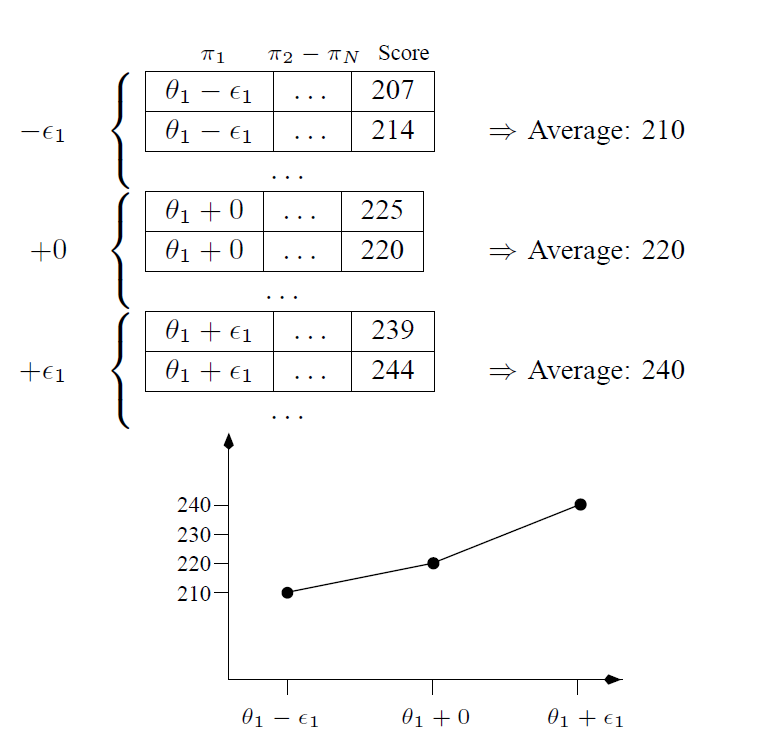
\includegraphics[width=0.5\textwidth]{figures/l9-training-diff.png}\\
  \caption{The policy updates}\label{fig:training-diff}
  \end{centering}
\end{figure}




\subsection{AlphaGo}

AlphaGo and its successor AlphaGo Zero are the most advanced
computer Go players, and the first to beat the best professional
players. We will concentrate on AlphaGo. AlphaGo Zero has an
additional benefit that it does not have any prior information about
the game (mainly in the form of games between human experts).

The training has roughly three phases. The first phase learns from
from human games (played by experts). Those games are used to derive
a network SL (Supervised Learning) to predict next move of the
human, and a Rollout which is a simple but very fast prediction (3
orders faster than SL).

During phase two an RL network is trained. It is initialized with SL
weights, and is optimized on self-play against itself.

In phase three, a value network is trained to predict the winner of
the game (trained on the RL network self-play games). (See
Figure~\ref{fig:AlphaGo-arch}.)


\begin{figure}
  % Requires \usepackage{graphicx}
  \begin{centering}
  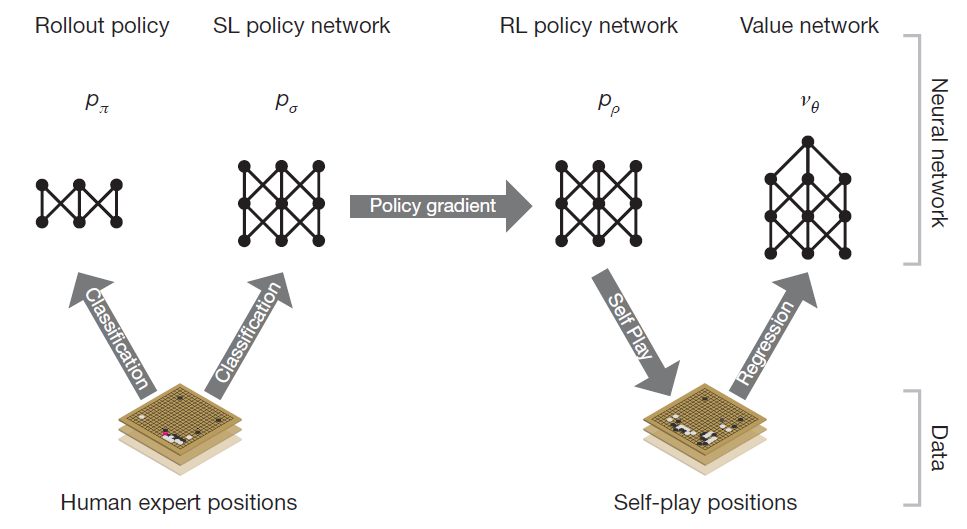
\includegraphics[width=\textwidth]{figures/AlphaGo-arch.PNG}\\
  \caption{The AlphaGo training process}\label{fig:AlphaGo-arch}
  \end{centering}
\end{figure}

\paragraph{Phase 1}\ \\
The SL network is trained to predict the human moves. It is a deep
network (13 layers), and the goal is to output
$p(\action|\state;\sigma)$ where $\sigma$ are the parameters of the
network. The parameters are update using a gradient step,
\[
\Delta \sigma \propto \frac{\partial \log
p(\action|\state;\sigma)}{\partial \sigma}
\]
Overall, this network increased the prediction accuracy (compared to
previous computer programs) from 44\% to 55\%. We should note that
the increase in accuracy translated to a much more significant
improvement in the performance.

In addition to SL, another very fast classifier Rollout was build.
It uses a linear function approximation and predicts using a
soft-max. The accuracy is only 24\% but it is much faster ($2\mu s$
compared to $3ms$,  a factor of $1500$).

\paragraph{Phase 2}\ \\
We learn an RL network that outputs $p(\action|\state;\rho)$ where
$\rho$ are the parameters of the network. The network structure is
identical to that of SL, and the RL is initialized to the weights of
SL, i.e., $\sigma$.

The RL is trained using self-play. Rather then playing against the
most recent network, the opponent is selected at random between the
recent RL configurations. This is done to avoid overfitting. The
rewards of the game are given only at the end (win or lose).

The training is done using SGD with policy gradient
\[
\Delta \rho \propto \frac{\partial \log
p(\action|\state;\rho)}{\partial \rho}
\]

The learned RL network outperformed SL (wins 80\%) of the games.
However, SL is better in predicting expert human behavior.

\paragraph{Phase 3}\ \\
We learn a value function $V(\state;\theta)$. The goal is to predict
the probability that RL will win, and it is trained on the self-play
data of RL. It uses a SGD update
\[
\Delta \theta \propto \frac{\partial V(\state;\theta)}{\partial
\theta}
\]

When the training was done on complete games, there was a serious
problem of over-fitting. (The training error was $0.19$ while the
test error was $0.37$). For this reason, the training is limited to
only one position per game. The error rate is about $0.22$.

The system uses a Monte-Carlo Search Trees (MCST) to evaluate the
positions. The tree is used to perform a lookahead. It uses the
Rollout policy to generate trajectory from the given position. The
prediction is an average of the value network prediction
$V(\state;\theta)$ and the outcome of the Rollout policy. To see a
run of the Monte-Carlo Search Tree see
Figure~\ref{fig:AlphaGo-MCST}.


\begin{figure}
  % Requires \usepackage{graphicx}
  \begin{centering}
  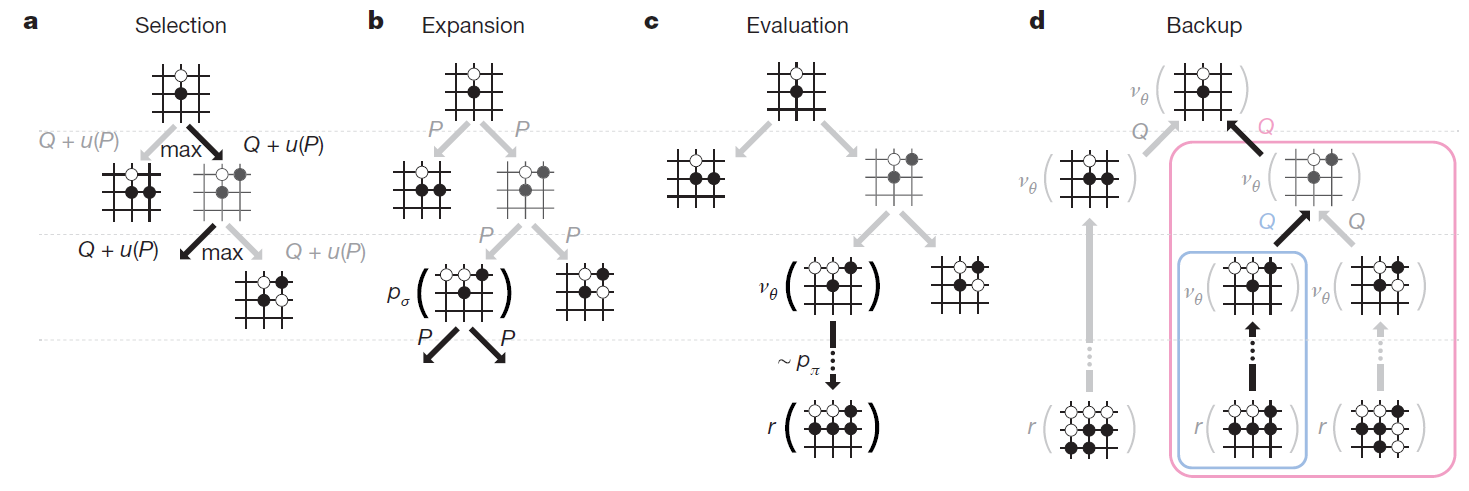
\includegraphics[width=\textwidth]{figures/AlphaGo-MCST.PNG}\\
  \caption{AlphaGo use of Monte-Carlo trees}\label{fig:AlphaGo-MCST}
  \end{centering}
\end{figure}

\section{Bibliography Remarks}

The training of Aibo for RoboSoccer is by \cite{KohlS04}.

The work on AlphaGo is by \cite{SilverHMGSDSAPL16}.

Part of the outline borrows from David Silver class notes and the
the book of Sutton and Barto \cite{SuttonB98}.


% \chapter{Large state space: tree based optimization}
% %\input{Lecture6}
% %\input{exercises4}

% %\chapter{Learning in Simple Bandits Problems}
% %\input{Lecture7}
% %\input{exercises5}


% \chapter{Deep RL}

% \chapter{ Multi-Arm bandits}
% \label{chapter:MAB}
% 

\section{Stochastic Bandits and Regret Minimization}

We consider a simplified model of an MDP where there is only a
single state and a fixed set $A$ of $k$ actions (a.k.a., arms). We
consider a finite horizon problem, where the horizon is $T$.
Clearly, the planning problem is trivial, simply select the action
with the highest expected reward. We will concentrate on the
learning perspective, where the expected reward of each action are
unknown.

At each round $1\leq t\leq T$ the player selects and executes an
action. After executing the action, the player observes the reward
of the action. However, the rewards of the other actions in $A$ are
not revealed to the player.

The reward for action $i$ at round $t$ is denoted by $r_{t}(i)\sim
D_{i}$, where the support of the reward distribution $D_{i}$ is
$[0,1]$. We assume that the rewards are i.i.d. (independent and
identically distributed).

\paragraph{Motivation}
\begin{enumerate}
\item \textbf{News}: a user visits a news site and is presented with a news
header. The user either clicks on this header or not. The goal of
the website is to maximize the number of clicks. So each possible
header is an action in a bandit problem, and the clicks are the
rewards
\item \textbf{Medical Trials}: Each patient in the trial is prescribed one
treatment out of several possible treatments. Each treatment is an
action, and the reward for each patient is the effectiveness of the
prescribed treatment.
\item \textbf{Ad selection}: In website advertising, a user visits a webpage,
and a learning algorithm selects one of many possible ads to
display. If an advertisement is displayed, the website observes
whether the user clicks on the ad, in which case the advertiser pays
some amount $v_{a} \in[0, 1]$. So each advertisement is an action,
and the paid amount is the reward.
\end{enumerate}

\paragraph{Model}
\begin{itemize}
\item A set of actions $A=\left\{ a_{1}\dots,a_{k}\right\} $
\item Each action $a_{i}$ has a reward distribution $D_{i}$ over
$[0,1]$.
\item The expectation of distribution $D_{i}$ is:
\[
\mu_{i}=E_{X\sim D_{i}}\left[X\right]
\]
\item $\mu^{*}= \max_{i}\mu_{i}$ and $a^*=\arg\max_i\mu_i$.
\item $a_{t}$ is the action the learner chose at round $t$
\[
Regret=\max_{i\in A}{\displaystyle
\sum_{t=1}^{T}\underbrace{r_{t}(i)}_{\text{Random
variable}}}-{\displaystyle
\sum_{t=1}^{T}\underbrace{r_{t}(a_{t})}_{\text{Random variable}}}
\]
\[
\begin{array}{ccc}
\text{Pseudo Regret} & = & {\displaystyle \max_{i}}E\left[{\displaystyle \sum_{t=1}^{T}r_{t}(i)}\right]-E\left[{\displaystyle \sum_{t=1}^{T}r_{t}(a_{t})}\right]\\
\\
 & = & \mu^{*}\cdot T-{\displaystyle \sum_{t=1}^{T}\mu_{a_{t}}}
\end{array}
\]
\end{itemize}

\ymignore{
\begin{leftbar}
\section{Sub-Gaussian Random Variable}

A random variable $X$ is called $\sigma^{2}-sub-gaussian$ if for any
$\lambda\in\mathbb{R}$:

\[
E\left[e^{\lambda X}\right]\le e^{\sigma^{2}\lambda^{2}/2}
\]

\paragraph{Examples}
\begin{enumerate}
\item $X\sim N\left(0,\sigma^{2}\right)$, $E\left[e^{\lambda X}\right]=e^{\sigma^{2}\lambda^{2}/2}$
$\Rightarrow$ X is $\sigma^{2}-sub-gaussian$
\item X s.t $\begin{cases}
E\left[X\right]=0\\
\left|X\right|\le B
\end{cases}$, then X is $B^{2}-sub-gaussian$
\end{enumerate}

\subsection{Properties of $\sigma^{2}-sub-gaussian$ random variable $X$}
\begin{itemize}
\item $E\left[X\right]=0$, $Var\left(X\right)\le\sigma^{2}$
\item $c\cdot X$ is $c^{2}\sigma^{2}-sub-gaussian$
\item If $X_{1}\dots,X_{m}$ are $\sigma^{2}-sub-gaussian$ then $S={\displaystyle \sum_{i=1}^{m}X_{i}}$
is $m\sigma^{2}-sub-gaussian$\\
 $\frac{1}{m}S=\frac{1}{m}{\displaystyle \sum_{i=1}^{m}X_{i}}$ is
$\frac{\sigma^{2}}{m}-sub-gaussian$
\end{itemize}

\begin{theorem}
\label{thm:sub-gaus}
Let X be $\sigma^{2}-sub-gaussian$ random
variable, then
$Pr[X\geqslant\epsilon]\le\exp(-\frac{\epsilon^{2}}{2\sigma^{2}})$.
\end{theorem}

\begin{proof}
\[
\begin{array}{ccc}
Pr[X\geqslant\epsilon] & = & Pr[e^{\lambda X}\geqslant e^{\lambda\epsilon}]\\
\\
 & \le & \frac{E[e^{\lambda X}]}{e^{\lambda\epsilon}}\\
\\
 & \le & \exp(\sigma^{2}\lambda^{2}/2-\lambda\epsilon)
\end{array}
\]
where we used Markov's inequality for the first stage and the fact
that the random variable is $\sigma^{2}-sub-gaussian$ for the
second.

If we choose $\lambda=\frac{\epsilon^{2}}{\lambda^{2}}$, then we
get:
\[
\begin{array}{ccc}
Pr[X\geqslant\epsilon] & \le & \exp(-\frac{\epsilon^{2}}{2\sigma^{2}})\end{array}
\]
\end{proof}
\end{leftbar}

\subsection{Hoeffding's inequality}
}

We will use extensively the following concentration bound.

\begin{theorem}[Hoeffding's inequality]
\label{thm:hoeffding}
%
Given $X_{1},\dots,X_{m}$ i.i.d random
variables s.t $X_{i}\in[0,1]$ and $E[X_{i}]=\mu$.
\[
\begin{array}{ccc}
Pr[\underbrace{\frac{1}{m}{\displaystyle \sum_{i=1}^{m}X_{i}-\mu}}_{\frac{1}{m}S}\ge\epsilon] & \le & \exp(-\frac{\epsilon^{2}m}{2})\end{array}
\]
\end{theorem}

\ymignore{
\begin{leftbar}
This is a direct conclusion from Theorem~\ref{thm:sub-gaus}. Let
$\bar{X_{i}}=X_{i}-\mu$. Using the facts that $E[\bar{X_{i}}]=0$
and:
\[
\begin{array}{ccc}
X_{i}\in[0,1] & \Rightarrow & |\bar{X_{i}|}\le1\\
\\
 & \Rightarrow & X_{i}\text{ is 1-sub-gaussian}
\end{array}
\]
\end{leftbar}
}

\subsection{Warmup: Full information $k=2$ }

We start with a simple case where there are two actions and we
observe the reward of both actions at each time $t$. We will analyze
the greedy policy, which selects the action with the higher average
reward (so far).

The greedy policy at time $t$ does the following:
\begin{itemize}
\item We observe $\big\langle r_{t}(1),r_{t}(2)\big\rangle$
\item Define
\[
avg_{t}(i)=\frac{1}{t} \sum_{\tau=1}^{t}r_{\tau}(i)
\]
\item In time $t+1$ we choose:
\[
a_{t+1}=\arg\max_{i\in\{1,2\}}avg_{t}(i)
\]
\end{itemize}


We now would like to compute the expected regret of the greedy
policy. W.l.o.g., we assume that $\mu_{1}\ge\mu_{2}$, and define
$\Delta=\mu_{1}-\mu_{2}\ge0$.
\[
\text{Pseudo Regret}= \sum_{t=1}^{\infty}(\mu_{1}-\mu_{2})
\Pr\left[avg_{t}(2)\ge avg_{t}(1)\right]
\]
Clearly, at any time $t$,
\[
E[avg_{t}(2)-avg_{t}(1)]=\mu_{2}-\mu_{1}=-\Delta
\]
We can define a random variable $X_t=r_t(2)-r_t(1)+\Delta$ and
$E[X_t]=0$. Since $(1/t)\sum_t X_t = avg_t(2)- avg_t(1)+\Delta$, by
Theorem~\ref{thm:hoeffding}
\[
Pr[S_2(t)\geq S_1(t)]= Pr\left[avg_{t}(2)-avg_{t}(1)+\Delta
\ge\Delta\right]\le e^{-\Delta^{2}\frac{t}{2}}
\]
We can now bound the regret as follows,

\begin{align*}
E\left[\text{Pseudo Regret}\right] & = &
 \sum_{t=1}^{\infty}\Delta\Pr\left[S_{2}(t)\ge S_{1}(t)\right]\\
 & \le &  \sum_{t=1}^{\infty}\Delta e^{-\Delta^{2}\frac{t}{2}}\\
 & \le &  \int_{0}^{\infty}\Delta e^{-\Delta^{2}\frac{t}{2}}dt\\
 & = & \left[\frac{2}{\Delta}e^{-\Delta^{2}\frac{t}{2}}\right]_{0}^{\infty}\\
 & = & \frac{2}{\Delta}
\end{align*}
Notice that this regret bound does not depend on $T$!

\subsection{Stochastic Multi-Arm Bandits}

%\subsection{Bandits}

We will now see that we cannot get a regret that does not depend on
$T$ for the bandits case. Considering the following example:
\[
a_{1}\sim Br\left(\frac{1}{2}\right)\]

For action $a_2$ there are two alternatives, each with probability
$1/2$,
\[
a_{2}\sim Br\left(\frac{1}{4}\right) \left(w.p. \frac{1}{2}\right)
\qquad or \qquad a_{2}\sim Br\left(\frac{3}{4}\right) \left(w.p.
\frac{1}{2}\right)
\]

Assume by way of contradiction
\[
E\left[ \sum_{i \in \{1,2\}} \Delta_i |T_i|\right] = E\left[Pseudo
Regret\right]=R
\]

where $R$ does not depend on $T$. \\ By Markov inequality:
\[
Pr\left[Pseudo Regret\ge2R\right]\le\frac{1}{2}
\]

Since $\mu_1$ is known, an optimal algorithm will first check $a_2$
in order to decide which action is better and stick with it.

Assuming $\mu_2 = \frac{1}{4}$, and the algorithm decided to stop
playing $a_2$ after $M$ rounds, Then:
\[
Pseudo Regret = \frac{1}{4}M
\]
Thus,
\[
Pr\left[Pseudo Regret\ge 2R \right] = Pr\left[ M\ge 8R
\right]\le\frac{1}{2}
\]
And,
\[
Pr\left[M < 8R \right]>\frac{1}{2}
\]
Hence, the probability that after $8R$ rounds, the algorithm will
stop playing $a_2$ (if $\mu_2 = \frac{1}{4}$) is at least
$\frac{1}{2}$. This implies that there is some sequence of $8R$
outcomes which will result is stopping to try action $a_2$. For
simplicity, assume that the sequence is the all zero sequence.

Assume $\mu_2 = \frac{3}{4}$, but all $8R$ first rounds, playing
$a_2$ yield the value zero (which happens with probability
$\left(\frac{1}{4}\right)^{8R}$). We assumed that after $8R$ zeros
for action $a_2$ the algorithm will stop playing $a_2$, even though
it is the preferred action. In this case, we will get:
\[
Pseudo Regret = \frac{1}{4} (T - M) \approx \frac{1}{4}T
\]

The expected Pseudo Regret is,
\[
E\left[Pseudo Regret\right] = R \geq
\underbrace{\frac{1}{2}}_{a_{2}\sim Pr(Br\left(\frac{3}{4}\right))}
\cdot \underbrace{\left(\frac{1}{4}\right)^{8R}}_{Pr(all \; 0 |
a_{2}\sim Pr(Br\left(\frac{3}{4}\right))} \cdot (T - 8R) \approx
e^{-O(R)}T
\]

Which implies that:
\[
R=\Omega\left(\log T\right)
\]
Contrary to the assumption that $R$ does not depend on $T$.
%\footnote{More formally, after $8R$ steps, there exists some
%sequence of outcomes that cause the algorithm to switch to action
%$a_2$. The probability of that sequence is at least
%$\left(\frac{1}{4}\right)^{8R}$.}

\topic{Explore-Then-Exploit}{random}

\begin{enumerate}
%
\item We choose a parameter $M$.
% time frame $kM$ to explore.
%
For $M$ phases we choose each action once (for a total of $kM$
rounds of exploration).
%
\item After $kM$rounds we always choose the action that had highest
average reward during the explore phase.
\end{enumerate}

Define:
\begin{align*}
T_{j}&= \left\{ t:a_t=j,t\le k\cdot M\right\}\\
\hat{\mu}_{j}&=\frac{1}{M} \sum_{t\in T_{j}}r_{j}(t)\\
\mu_{j}&=E[r_{j}(t)]\\
\Delta_{j}&=\mu^{*}-\mu_{j}
\end{align*}
where $\Delta_j$ is the difference in expected reward of action $j$
and the optimal action.

We can now write the regret as a function of those parameters:
\[
E\left[\text{Pseudo regret}\right]=\underbrace{{\displaystyle
\sum_{j=1}^{k}\Delta_{j}\cdot
M}}_{Explore}+\underbrace{\left(T-k\cdot M\right){\displaystyle
\sum_{j=1}^{k}\Delta_{j}Pr\left[j=\arg\max_{i}\hat{\mu}_{i}\right]}}_{Exploit}
\]

For the analysis define:
\[
\lambda=\sqrt{\frac{8\log T}{M}}
\]

By Theorem~\ref{thm:hoeffding} we have
\[
\Pr\left[\left|\hat{\mu}_{j}-\mu_{j}\right|\ge\lambda\right]  \le
2e^{-\frac{\lambda M}{2}}=\frac{2}{T^{4}}
\]
which implies (using the union bound) that
\[
\Pr\underbrace{\left[\exists_{j}:\left|\hat{\mu}_{j}-\mu_{j}\right|\ge\lambda\right]}_{B}
 \le  \frac{2k}{T^{4}}\underset{for\,k\leq T}{\leq}\frac{2}{T^{3}}
\]

Define the ``bad event''
$B=\{\exists_{j}:\left|\hat{\mu}_{j}-\mu_{j}\right|\ge\lambda\}$. If
$B$ did not happen then for each action $j$, such that
$\hat{\mu}_{j}\ge\hat{\mu}^{*}$, we have
\[
\mu_{j}+\lambda\ge\hat{\mu}_{j}\ge\hat{\mu}^{*}\ge\mu^{*}-\lambda
\]
therefore:
\[
2\lambda\ge\mu^{*}-\mu_{j}=\Delta_{j}
\]
and therefore:
\[
\Delta_{j}\le2\lambda
\]

Then, we can bound the expected regret as follows:
\begin{align*}
E[PseudoRegret] & \leq  \underbrace{\left({\displaystyle
\sum_{j=1}^{k}\Delta_{j}}\right)M}_{Explore}+\underbrace{\left(T-k\cdot
M\right)\cdot2\lambda}_{\text{B didn't
happen}}+\underbrace{\frac{2}{T^{3}}\cdot T}_{\text{B happened}}\\
 & \leq  k\cdot M+2\cdot\sqrt{\frac{8\log T}{M}}\cdot T+\frac{2}{T^{2}}
\end{align*}

If we optimize the number of exploration phases $M$ and choose $M=T^{\frac{2}{3}}$,
we get:
\[
k\cdot T^{\frac{2}{3}}+2\cdot\sqrt{8\log T}\cdot
T^{\frac{2}{3}}+\frac{2}{T^{2}}
\]
which is sub-linear but more than the $O(\sqrt{T})$ rate we would
expect.

\section{Improved Regret Minimization Algorithms}

We will look at some more advanced algorithms that mix the
exploration and exploitation.

Define:

$n_{t}(i)$ - the number of times we chose action $i$ by round $t$

$\hat{\mu}_{t}(i)$ - the average reward of action $i$ so far, that
is:
\[
\hat{\mu}_{t}(i)={\displaystyle
\sum_{t=1}^{T}r_{i}(t)}\mathbb{I}\left(a_{t}=i\right)\frac{1}{n_{i}(t)}
\]
Notice that $n_{i}(t)$ is a random variable and not a number!

We would like to get the following result:
\[
\Pr\left[\left|\hat{\mu}_{t}(i)-\mu_{i}\right|\le\underbrace{\sqrt{\frac{8\log
T}{n_{i}(t)}}}_{\lambda_{t}(i)}\right]\ge1-\frac{2}{T^{4}}
\]

We would like to look at the $m^{th}$ time we sampled action $i$:
\[
\hat{\mathbb{V}}_{m}(i)=\frac{1}{m} \sum_{\tau=1}^{m}r_{i}(t_{\tau})
\]
Where the $t_{\tau}$'s are the rounds when we chose action $i$

Now we fix $m$ and get:
\[
\forall{i}\forall{m}\;\;\;
\Pr\left[\left|\hat{\mathbb{V}}_{m}(i)-\mu_{i}\right|\le\sqrt{\frac{8\log
T}{m}}\right]\ge1-\frac{2}{T^{4}}
\]
and notice that $\hat{\mu}_{t}(i)\equiv\hat{\mathbb{V}}_{i}(m)$ when
$m=n_{i}(t)$.

Define the ``good event'' $G$:
\[
G=\left\{ \forall_{i}\forall_{t}\left|\hat{\mu}_{i}(t)-\mu_{i}\right|\le\lambda_{i}(t)\right\}
\]
The probability of $G$ is,
\[
Pr\left(G\right)\ge1-\frac{2}{T^{2}}
\]

\section{Refine Confidence Bound}

Define the upper confidence bound:
\[
UCB_{t}(i)=\hat{\mu}_{t}(i)+\lambda_{t}(i)
\]
and similarly, the lower confidence bound:
\[
LCB_{t}(i)=\hat{\mu}_{t}(i)-\lambda_{t}(i)
\]
if $G$ happened then:
\[
\forall{i}\forall{t}\;\;\;\mu_{i}\in\left[LCB_{t}(i),UCB_{t}(i)\right]
\]
Therefore:
\[
Pr\biggl[\forall{i}\forall{t}\;\;\;
\mu_{i}\in\left[LCB_{t}(i),UCB_{t}(i)\right]\biggr]\ge1-\frac{2}{T^{2}}
\]

\subsection{Successive Elimination}

We maintain a set of actions S.

Initially $S=A$

In each phase:
\begin{itemize}
\item We try every $i\in S$ once
\item For each $j\in S$ if there exists $i\in S$ such that:
\[
UCB_{t}(j)<LCB_{t}(i)
\]
 We remove $j$ from $S,$ that is we update:
\[
S\leftarrow S-\left\{ j\right\}
\]
\end{itemize}
We will get the following results:
\begin{itemize}
\item As long as action $i$ is still in $S$, we have tried action $i$ exactly the
same number of times as all of any other action $j\in S$.
\item The best action, under the assumption that the event $G$ holds, is never eliminated
from $S$.
\end{itemize}
Under the assumption of $G$ we get:

\[
\mu^{*}-2\lambda\le\hat{\mu}^{*}-\lambda=LCB_{*}<UCB_{i}=\hat{\mu_{i}}+\lambda\leq\mu_{i}+2\lambda
\]

Where $\lambda=\lambda_{i}=\lambda^{*}$ because we have chosen
action $i$ and the best action the same number of times so far.

Therefore, assuming event $G$ holds,
\[
\Delta_{i}=\mu^{*}-\mu_{i}\le4\lambda=4\sqrt{\frac{8\log
T}{n_{t}(i)}}
\]
\[
\Rightarrow\;\;\; n_{T}(i)\le\frac{c}{\Delta_{i}^{2}}\log T
\]

This implies that
\begin{align*}
E\left[\text{Pseudo Regret}\right]  = &  \sum_{i=1}^{k}\Delta_{i}n_{i}(t)\\
  \le &  \sum_{i=1}^{k}\frac{c}{\Delta_{i}}\log T
  +\underbrace{\frac{2}{T^{2}}\cdot T}_{\text{The bad event}}
\end{align*}

meaning that the expected pseudo regret is bounded by $O\left(\frac{1}{T}\right)$.

\subsection{Upper confidence bound (UCB)}

The UCB algorithm simply uses the UCB bound. The algorithm works as
follows:
\begin{itemize}
\item We try each action once (for a total of $k$ rounds)
\item Afterwards we choose:
\end{itemize}
\[
a_{t}=\arg\max_{i}UCB_t(i)
\]

If we chose action $i$ then, assuming $G$ holds, we have
\[
UCB_{t}(i)  \ge  UCB_t(a^*)\geq\mu^{*}
\]
where $a^*$ is the optimal action.

Using the definition of UCB and the assumption that $G$ holds, we
have
\[
UCB_t(i)=\hat{\mu}_{t}(i)+\lambda_{t}(i)\le\mu_{i}+2\lambda_{t}(i)
\]
Since we selected action $i$ at time $t$ we have
\[
\mu_{i}+2\lambda_{t}(i)\ge\mu^{*}
\]
Rearranging, we have,
\[
2\lambda_t(i)\ge\mu^{*}-\mu_{i}=\Delta_{i}
\]
Each time we chosen action $i$, we could not have made a very big
mistake because:
\[
\Delta_{i}\leq\text{ }2\cdot\sqrt{\frac{8\log T}{n_{t}(i)}}
\]

And therefore if $i$ is very far off from the optimal action we
would not choose it too many times. We can bound the number of time
action $i$ is used by,
\[
n_{t}(i)\leq\frac{c}{\Delta_{i}^{2}}\log T
\]

And over all we get:
\begin{align*}
E\left[\text{Pseudo Regret}\right] & =
\sum_{i=1}^{k}\Delta_{i}E\left[n_{t}(i)\right]+\underbrace{\frac{2}{T^{2}}\cdot
T}_{\text{The bad event}}
\\
 & \le  \sum_{i=1}^{k}\frac{c}{\Delta_{i}}\cdot\log T+\frac{2}{T}
\end{align*}

\section{Best Arm Identification}

We would like to identify the best action, or an almost best action.
We can define the goal in one of two ways.

\paragraph{PAC criteria }
An action $i$ is $\epsilon$-optimal if  $\mu_i\geq \mu^*-\epsilon$. The PAC criteria is
that, given $\epsilon,\delta>0,$, with probability at least
$1-\delta$, find an $\epsilon$ optimal action.

\paragraph{Exact identification}
Given $\Delta\le\min_{i\neq a^*}\mu^{*}-\mu_{i}$ (for every suboptimal action $i$),
find the optimal action $a_{*}$, with probability at least
$1-\delta$.

\subsection{Naive Algorithm (PAC criteria):}

We sample each action $i$ for
$m=\frac{8}{\epsilon^{2}}\log\frac{2k}{\delta}$ times, and return
$a= \arg\max_{i}\hat{\mu}_{i}$ .

For rewards in $[ 0 ,1]$, then, by Theorem \ref{thm:hoeffding}, for
every action $i$ we have
\[
Pr\left[\underbrace{\left|\hat{\mu}_{i}-\mu_{i}\right|>\frac{\epsilon}{2}}_{\text{bad
event}}\right]\le 2
e^{-\left(\frac{\epsilon}{2}\right)^{2}m/2}=\frac{\delta}{k}
\]
By union bound we get:
\[
Pr\left[\exists_{i}\left|\hat{\mu}_{i}-\mu_{i}\right|>\frac{\epsilon}{2}\right]\le\delta
\]

If the bad event
$B=\{\exists_{i}\left|\hat{\mu}_{i}-\mu_{i}\right|>\frac{\epsilon}{2}\}$
did not happen, then both: (1)
$\mu^{*}-\frac{\epsilon}{2}\le\hat{\mu}^{*}$ and (2)
$\mu_{i}+\frac{\epsilon}{2}\le\hat{\mu}_{i}$.

This implies,
\[
\Rightarrow\text{ }\mu_{i}+\frac{\epsilon}{2}\ge\hat{\mu}_{i}\ge\hat{\mu}^{*}\ge\mu^{*}-\frac{\epsilon}{2}
\]
\[
\Rightarrow\text{ }\epsilon\ge\mu^{*}-\mu_{i}
\]

And therefore $a={\displaystyle \arg\max_{i}\hat{\mu}_{i}}$ is the
optimal action in probability $1-\delta$.

We would like to slightly improve the sample size of this algorithm

\subsection{Median Algorithm}

The idea: the algorithm runs for $l$ phases, after each phase we
eliminate half of the actions. This elimination allows us to sample
each action more times in the next phase which makes eliminating the
optimal action less likely.

\begin{algorithm}
\textbf{Input}: $\epsilon,\delta>0$

\textbf{Output}: $\bar{a}\in A$

\textbf{Init}: $S_{1}=A$, $\epsilon_{1}=\frac{\epsilon}{4}$,
$\delta_{1}=\frac{\delta}{2}$, $l=1$

\textbf{Repeat}:

~~~~~~$\forall_{i}\in S_{l}$, sample action i, $\frac{1}{\left(\frac{\epsilon_{l}}{2}\right)^{2}}\log\left(\frac{3}{\delta_{l}}\right)$
times

~~~~~~$\hat{\mu}_{i}\leftarrow\text{mean (only of samples during the \ensuremath{l^{th}}phase)}$

~~~~~~$\text{median}_{l}\leftarrow median\left\{ \hat{\mu}_{i}:i\in S_{l}\right\} $

~~~~~~$S_{l+1}\leftarrow\left\{ i\in S_{l}:\hat{\mu}_{i}\ge\text{median}_{l}\right\} $

~~~~~~$\epsilon_{l+1}\leftarrow\frac{3}{4}\epsilon_{l}$

~~~~~~$\delta_{l+1}\leftarrow\frac{\delta_{l}}{2}$

~~~~~~$l\leftarrow l+1$

\textbf{Until} $\left|S_{l}\right|=1$

\caption{Best Arm Identification}
\end{algorithm}

\paragraph{Complexity:}

During phase $l$ we have $\left|S_{l}\right|=\frac{k}{2^{l-1}}$
actions.
\[
\epsilon_{l}=\frac{3}{4}\epsilon_{l-1}=\frac{\epsilon}{4}\left(\frac{3}{4}\right)^{l-1},\text{
}\delta_{l}=\frac{\delta}{2^{l}}
\]
\[
\Rightarrow\text{ }{\displaystyle \sum\epsilon_{l}\le\epsilon},\text{ }{\displaystyle \sum\delta_{l}\le\delta}
\]

The total number of samples is therefore:

\begin{align*}
 \sum_l |S_l| \cdot \frac{4}{\epsilon_l^2}\log \frac{3}{\delta_l} &=
\sum_{l}\frac{k}{2^{l-1}}\frac{64}{\epsilon^{2}}\left(\frac{16}{9}\right)^{l-1}\log\frac{3\cdot2^{l}}{\delta}\\
& =  {\displaystyle \sum_{l}k\left(\frac{8}{9}\right)^{l-1}\left[c\cdot\frac{\log\frac{1}{\delta}}{\epsilon^{2}}+\frac{\log3}{\epsilon^{2}}+\frac{l}{\epsilon^{2}}\right]}\\
\\
 & =  O\left(\frac{k}{\epsilon^{2}}\log\frac{1}{\delta}\right)
\end{align*}


\paragraph{Correctness:}

\begin{theorem}
$Pr\left[\underbrace{{\displaystyle \max_{j\in
S_{l}}\mu_{j}}}_{\text{action
\ensuremath{l}}}\le\underbrace{{\displaystyle \max_{j\in
S_{l+1}}\mu_{j}}}_{\text{action
\ensuremath{l+1}}}+\epsilon_{l}\right]\ge1-\delta_{l}$
\end{theorem}

\begin{proof}
%We do the proof for $l=1$, general $l$ is similar. 
Let $\mu^*_l=\max_{j\in S_l} \mu_j$.
Define $E_{l}=\left\{\hat{\mu}^{*}_l<\mu^{*}_l-\frac{\epsilon_{1}}{2}\right\}$.
We have  $Pr\left[E_{l}\right]\le\frac{\delta_{l}}{3}$. If $E_{l}$ did not happen, we define a bad set:
\[
\text{Bad}=\left\{ j\text{ }:\text{ }\mu^{*}-\mu_{j}\ge\epsilon_{l},\text{ }\hat{\mu}_{j}\ge\hat{\mu}^{*}\right\}
\]
Consider an action $j$ such that $\mu^*-\mu_j\geq \epsilon_l$, then:
\[
Pr[\hat{\mu}_{j}\geq
\hat{\mu}^{*}|\underbrace{\hat{\mu}^{*}\ge\mu^{*}-\frac{\epsilon_{1}}{2}}_{\urcorner
E_{l}}\big] \le
Pr[\hat{\mu}_{j}\ge\mu_{j}+\frac{\epsilon_{1}}{2}|\urcorner E_{l}]
\le  \frac{\delta_{1}}{3}
\]
Note that the probability is not negligible. We will show that it cannot happen to too many such actions. We will bound the expectation of the size of $Bad$,
\[
E[|\text{Bad}||\urcorner E_{l}]\le k\frac{\delta_{1}}{3}
\]
 with Markov's inequality we get:
\[
Pr\left[\left|\text{Bad}\right|\ge\frac{k}{2}\right|\urcorner E_{l}]
 \le  \frac{E\left|\text{Bad}\right|}{k/2}
  =  \frac{2}{3}\delta_{l}
\]
 with probability $1-\delta_{l}$: $\hat{\mu}^{*}\ge\mu^{*}-\frac{\epsilon_{1}}{2}$ and $\left|\text{Bad}\right|\le\frac{k}{2}$. Therefore: $\exists_{j}\notin\text{Bad}$ and $j\in S_{l+1}$.
\end{proof}

% %\end{document}



% \chapter{POMDP}
% \label{chapter:POMDP}
% 
The lecture today is about Partially Observable MDP (POMDP). The
main difference is that we will not observe the current state but
only a signal that depends on it.


\paragraph{Example:}\ \\
Assume we have four states, in linear order: $1,2,3,4$. We have an
action UP that with probability $0.90$ moves from $i$ to $i-1$ and
with probability $0.1$ moves to $i+1$. Similarly, we have an action
DOWN that with probability $0.90$ moves from $i$ to $i+1$ and with
probability $0.1$ moves to $i-1$. (In state $i=1$ if we need to move
to $i-1$ we stay in $i=1$ and in state $i=4$ if we need to move to
$i+1$ we stays in state $i=4$.)

One of the states, state $2$ has a reward, while the other states do
not have any reward. (See Figure~\ref{fig:Example-4states}.) The
only observation we see is the reward.

Initially, we know we are in a random state without a reward. This
implies that the distribution of where we are is $(1/3,0,1/3,1/3)$.
Assume we did an action UP and did not observe a reward. We now can
compute the posterior of our probability distribution.

First, we compute the state probability distribution, assuming any
current state.
\begin{enumerate}
\item
Assuming we are in state $i=1$, our state distribution will be
$(0.9,0.1,0,0)$.
\item
Assuming we are in state $i=2$, our state distribution will be
$(0.9,0,0.1,0)$.
\item
Assuming we are in state $i=3$, our state distribution will be
$(0,0.9,0,0.1)$.
\item
Assuming we are in state $i=4$, our state distribution will be
$(0,0,0.9,0.1)$.
\end{enumerate}

Since our prior state distribution was $(1/3,0/1/3,1/3)$ our
posterior state distribution (before observing the reward) is
$(0.3,1/3,0.3,1/15)$.

Given that we observed ``no reward'' we are not instate $2$ so the
posterior state distribution is $(0.45,0,0.45,0.1)$.


\begin{figure}
  % Requires \usepackage{graphicx}
  \begin{centering}
  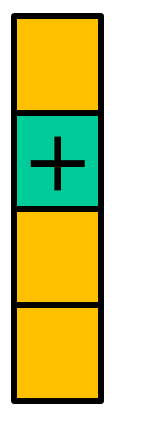
\includegraphics[width=0.1\textwidth]{figures/Example-4states.PNG}\\
  \caption{The four state POMDP}\label{fig:Example-4states}
  \end{centering}
\end{figure}


\section{POMDP: model}

The model of a POMDP will be similar to that of an MDP with an
additional observation function. Namely,
\begin{itemize}
\item
$S$, a finite set of states.
\item
$A$, a finite set of actions.
\item
$p(s'|s,a)$, a probability distribution of next state given that we
are in state $s$ and do action $a$.
\item
$R(s,a)$ a random variable for the reward in state $s$ doing action
$a$, and $r(s,a)=E[R(s,a)]$.
\item
$q_0$ the initial state (can also be a distribution over states)
\item
$Ob$ is an observability distribution over $O$ a set of observable
signals. $O$ can be either finite of infinite. $Ob(o|s',a)$ is the
probability that we observe signal $o\in O$ if we reach state $s'$
after doing action $a$. (Note that in an MDP we have the observable
signals $O=S$ and $Ob(o|s',a)=s')$.
\end{itemize}

\subsection{Belief state}

The belief state tracks the state distribution, which captures our
current state. Each time we perform an action and observe an
observation we compute a new belief state, which is our posterior
distribution, given our action and observation.

The belief state is a sufficient statistics, implying that it has
all the information needed from the history. (Also, two histories
which reach the same belief state, we should behave identical for
them.)
%
Formally, a belief state $b$ is a distribution over states, i.e.,
$b\in[0,1]^{|S|}$ and $\sum_s b(s)=1$.

Given a belief state $b$ and an action $a$ and observation $o$, we
need to compute the next belief state $b'(s)=\Pr[s'|o,a,b]$. This
will be a deterministic function, and we will have $b'=T(b,a,o)$.

\paragraph{Belief state computation:}\ \\
We compute the next belief state as follows:
\begin{align*}
b'(s') &= \Pr[s'|o,a,b]\\
&= \frac{\Pr[o|s',a,b]\Pr[s'|a,b]}{\Pr[o|a,b]}\\
&= \frac{\Pr[o|s',a]\sum_s \Pr[s'|a,b,s]\Pr[s|a,b]}{\Pr[o|a,b]}\\
&= \frac{Ob(o|s',a)\sum_s p(s'|a,s)b(s)}{\Pr[o|a,b]}
\end{align*}
where the first identity is the definition of the new belief state.
The second identity is Bayes rule. The third identity is adding a
conditioning over $s$. The last identity is translating the
probabilities to the POMDP parameters.

\paragraph{From POMDP to infinite MDP}\ \\
Consider the following MDP. The set of states are $B$ all the
possible belief states. (Note that $B$ is infinite!) The set of
actions is $A$ (finite). For each belief state $b$ and action $a$ we
define the expected reward $r(b,a)=\sum_s b(s)r(s,a)$. The
transition probability is to move to $b'=T(b,a,o)$ and is
deterministic. (Namely, $\Pr[b'=T(b,a,o)|b,a,o]=1$ and $\Pr[b'\neq
T(b,a,o)|b,a,o]=0$.)


\section{Value function}
The value function will be mapping belief states to expected return.
The return can be any of the return we discussed: finite horizon,
discounted, of average reward.

We would like to characterize the optimal value function. For a
finite horizon it will be piece-wise linear and convex. (For
discounted it will be convex.) Our algorithmic challenge is to
handle the infinite state spaces. We will concentrate on the case of
finite horizon.

For simplicity, we start with a horizon of length $H=1$. Namely, we
would like to maximize our immediate reward. For each action, our
immediate reward is a linear function in the belief state. Namely,
$r(b,a)=\sum_s b(s)r(s,a)$. The optimal action for $H=1$ is the
action $a$ that maximizes the expected reward. Namely,
$V^*_1(b)=\max_a r(b,a)=\max_a [\sum_s b(s)r(s,a)]$. This implies
that the optimal value function is a maximum of linear functions.
This gives us a finite representations. It also partitions the space
of belief states to regions, which in each region there is an
optimal action. The partition to the regions is done by intersecting
hyper-planes. The region in which $a_1$ is the best action is define
by $\{b: \forall a\neq a_1 \sum_s b(s)r(s,a_1)\geq \sum_s
b(s)r(s,a)\}$.

We will now consider a horizon of $H=2$. We will partition the task
to three steps. In the first step, we will assume that we are in
belief state $b$ perform action $a_1$ and observe $o_1$. In the
second step, we assume we are in belief state $b$ and perform action
$a_1$. In the third step, we only assume we are in belief state $b$.

Assume we  we are in belief state $b$ perform action $a_1$ and
observe $o_1$. We would like to compute $V_H(b|a_1,o_1)$ for $H=2$.
For the first step, given that we do action $a_1$, we can compute
the expected immediate reward $\sum_s b(s)r(s,a_1)$. Now, we move
from belief state $b$ to belief state $b'=T(b,a_1,o_1)$. When we
reach $b'$ we have only one step remaining, so we perform the best
action and get $V^*_1(b')$. This implies that
$V^*_2(b|a_1,o_1)=r(b,a_1)+V^*_1(b')$. (See
Figure~\ref{fig:belief-state-1}.) This implies that
$V^*_2(b|a_1,o_1)$ is piece-wise linear.

\begin{figure}
  % Requires \usepackage{graphicx}
  \begin{centering}
  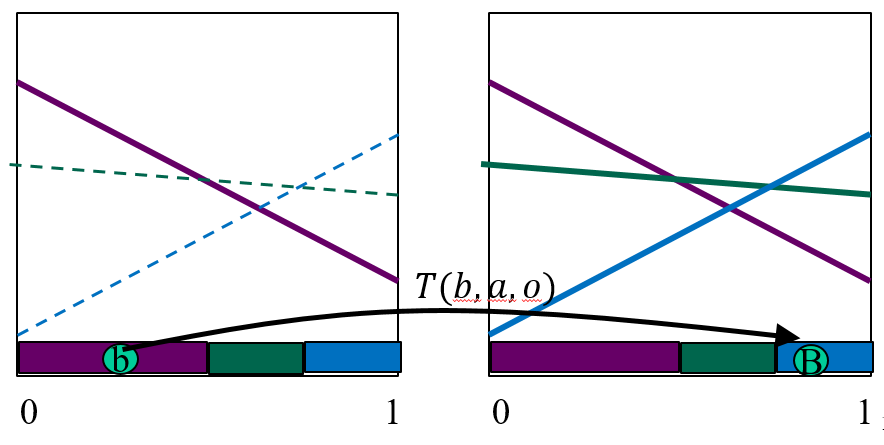
\includegraphics[width=0.5\textwidth]{figures/belief-state-1.PNG}\\
  \caption{Computing $V^*_2(b|a_1,o_1)$}\label{fig:belief-state-1}
  \end{centering}
\end{figure}

We can now do the same for each possible observations (assume the
set of observations is finite, for simplicity). This implies that we
have the values of $V^*_2(b|a_1,o)$ for any $o\in O$. This allows us
to compute $V^*_2(b|a_1)$, by simply averaging over the
observations. $V^*_2(b|a_1)=\sum_o V^*_2(b|a_1,o)\Pr[o|b,a_1]$. We
can compute $\Pr[o|b,a]=\sum_{s,s'} b(s)p(s'|s,a)Ob(o|s',a)$.

Given that we can compute $V_2^*(b|a)$ for any action $a\in A$, we
can deduce $V_2^*(b)=\max_a V_2^*(b|a)$.

We can now compute for a longer horizon, say $H=3$, using dynamic
programming. We want to compute $V^*_3(b)$. We first compute the
function $V_2^*(\cdot)$. For each action $a_i$ and observation $o_j$
we compute $V^*_3(b|a_i,o_j)$. This is done by first computing
$r(b,a_i)$ and $b'=T(b,a_i,o_j)$. Then we compute $V^*_3(b|a_i,o_j)
= r(b,a_i)+V^*_2(b')$.

\paragraph{Optimal value function}\ \\
For the finite horizon the optimal value function $V^*_H(b)$ is
define as follows,
\[
V^*_H(b)=\max_a [r(b,a)+\sum_o \Pr[o|b,a]V^*_{H-1}(T(b,a,o))]
\]
and the optimal policy is
\[
\pi_H^*(b)=\arg\max_a [r(b,a)+\sum_o \Pr[o|b,a]V^*_{H-1}(T(b,a,o))]
\]

\begin{theorem}
For the finite horizon, the function $V^*_H$ is piece-wise linear
and convex. In addition, there exists a collection of
$\Theta=\{\theta_i\in \mathbb{R}^{|S|}\}$ such that
$V^*_H(b)=\max_{\theta_i\in\Theta} \sum_s b(s)\theta_i(s)$.
\end{theorem}

For the discounted setting we have
\[
V^*(b)=[r(b,a)+\gamma\sum_o \Pr[o|b,a]V^*_{H-1}(T(b,a,o))]
\]
\begin{theorem}
For the discounted return, the function $V^*$ is convex.
\end{theorem}

\paragraph{Policy Tree}\ \\
How does the optimal finite horizon policy can be implemented. We
can create a tree. In each node of the tree, we can label it by the
action we perform. We label the outgoing edges by the observation we
receive. We start at the root. The action at the root is the action
we perform at the initial state. Given the observation we receive,
we continue to the next node in the tree. The label of that node is
the action we perform and so on. The depth of the tree is $H$ for a
finite horizon of length $H$.

\subsection{Value Iteration:}

We can run a value iteration in the POMDP (actually, on the belief
states. We can write the update as follows:
\begin{align*}
V^{a,o}_{t}(b)=&\frac{r(b,a)}{|O|}+\gamma\Pr[o|b,a]V_t(T(b,a,o))\\
V_{t}^a(b)=&\sum_o V^{a,o}_{t}(b)\\
V_{t+1}^*(b)=&\max_a V_{t}^a(b)\\
V_{t+1}^*(b) =& \max_a [r(b,a)+\gamma\sum_o V_t^*(T(b,a,o)
\end{align*}
%\begin{align*}
%V_{t+1}^*(b) =& \max_a [r(b,a)+\gamma\sum_o V_t^*(T(b,a,o)\\
%V_{t+1}^*(b)=&\max_a V_{t}^a(b)\\
%V_{t}^a(b)=&\sum_o V^{a,o}_{t}(b)\\
%V^{a,o}_{t}(b)=&\frac{r(b,a)}{|O|}+\gamma\Pr[o|b,a]V_t(T(b,a,o))
%\end{align*}

Assume that $V_t$ is piece-wise linear. Namely, there exists a set
$\Theta_t$ such that
\[
V_t(b)=\max_{\theta\in\Theta_t}\theta^\top b
\]
For $V_t^{a,o}$ we have that $b'=T(b,a,o)$ is linear in $b$, i.e.,
there is a matrix $M$ such that $b'=Mb$. (Note that $M$ depends on
$a$ and $o$.) The value of $V_t^{a,o}$ is
\[
V_t^{a,o}(b')=\max_{\theta\in\Theta_t} \theta^\top b'=
\max_{\theta\in\Theta_t} \theta^\top M b
\]
This implies that we can define $\Theta_t^{a,o}=\{\theta^\top
M:\theta \in \Theta_t\}$.

For $V^a_t$ we have that
\[
V_t^a(b)=\sum_o V_t^{a,o}(b)=\sum_o \max_{\theta\in\Theta_t^{a,o}}
\theta^\top b=\max_{\theta\in\Theta_t^{a}}\sum_o  \theta^\top b
\]
where
\[
\Theta^a_t=\{\sum_o
\theta^{a,o}|\theta^{a,o}\in\Theta^{a,o}_t\}
\]

For $V_{t+1}^*$ we have
\[
V^*_{t+1}(b)=\max_a V_t^a(b)=\max_{\theta\in\Theta_{t+1}}
\theta^\top b
\]
where $\theta_{t+1}=\cup_a \Theta^a_t$.
%

The complexity of value iteration depends on $\Theta_t$. For each
action $a$ and observation $o$ we have $|\Theta^{a,o}_t|\leq
|\Theta_t|$. For each action $a$ we have $|\Theta^a_t|\leq
{|\Theta^{a,o}_t|}^{|O|}\leq {|\Theta_t|}^{|O|}$. For $\Theta_{t+1}$
we have $|\Theta_{t+1}|\leq \sum_a |\Theta_t^a|\leq |A|\cdot
|\Theta_t|^{|O|}$.

The complexity is exponential in $|O|$ in each iteration! Pruning
can help, but the exponential time seems unavoidable.

\subsection{Hardness}

Many computational problems related to POMDPs are hard. For the
finite horizon, even with a unique start state, it is P-SPACE
complete to compute the return of the optimal policy.

For the finite horizon, in the case that there are no observations,
it is NP complete to compute the return of the optimal policy. (We
will show this simple hardness result.)

Assume we have no observations. This implies that we need to compute
a sequence of $H$ actions. The optimal policy will be the sequence
of $H$ actions that will maximize the return. We will show a
reduction to SAT.

Given a SAT formula over $n$ variables we create the following
POMDP. For each clause we create the following POMDP gadget. We have
always two actions $0$ and $1$. We create two lines of length $n$,
one line ends in a state with reward $1$ and the other in a state
with reward $0$. All other rewards will be zero. We ``think'' of the
state in the line as a number in $[1,n]$ and we associate the state
$i$ it with the variable $x_i$.

We start at the line ending with $0$. All the transition of states
in the line ending in $1$ simply continue to the next state, i.e.,
from $i$ to $i+1$ (for both actions). For the line ending in zero,
for each state $i$ where $x_i$ nor $\bar{x}_i$ do not appear in the
clause, we continue to the next state on this line, with both
actions.

For state $i$ in the line that ends in $0$, if $x_i$ appears
 in the clause, then in state $s_i$ with action $1$ we
move to the $i+1$ state in the line ending in $1$, and with action
$0$ we move to state $i+1$ in the line ending in zero.
%
Similarly, if $\bar{x}_i$ appears in the clause,  then in state
$s_i$ with action $0$ we move to the $i+1$ state in the line ending
in $1$, and with action $1$ we move to state $i+1$ in the line
ending in zero.

It is not hard to see that the sequence of $n$ actions will lead to
the reward $1$ if and only if it represents an satisfying assignment
to the clause.

We now take the gadgets for all the clauses, and select our initial
state to uniformly at random to be the start state of one of the
gadget (which represent a clause).

If the SAT formula is satisfiable, there is an assignment that
satisfies all the clauses. Therefore guarantees a return of $1$.

Otherwise for each sequence of action, which represent an
assignment, there is some clause which is not satisfied. This
implies that the return is at most $1-1/m$, where $m$ is the number
of clause.

\paragraph{Remark:} Actually, we can get from the same reduction
also a hardness to approximate result. We simply consider the
MAX-SAT problem. For 3-SAT it is NP-hard to decide distinguish
between satisfying $7/8+\epsilon$ of the terms or all the terms.
This implies that it is NP-hard to distinguish between a return of
$7.8+\epsilon$ or $1$.

\subsection{Policy Plan: Automata}

A simple class to describe the policy is a finite automata with
output, which is called a Moore automata. The outputs will be the
selected actions and the inputs are the observations. While it is
true that this class of policies is not universal, namely, not any
policy can be represented in this way, many policies can be.

One nice observation regarding this class of polices is that we can
efficiently compute the value function of a given automata. Assume
that $\pi$ is described by an automata. The value of $\pi$ from
state $s$ when its automata is in state $\sigma$ is
\[
V^\pi(s;\sigma)=r(s,a)+\gamma \sum_{o,s'}
p(s'|s,a)Ob(o|s'a)V^\pi(s';\sigma')
\]
where $a=\pi(\sigma,o)$ the action selected by $\pi$ when in state
$\sigma$ of the automata and observes $o$, and $\sigma'$ is the next
state in the automata, given we are in state $\sigma$ and observe
$o$.

This implies that we have a set of linear equations and we can solve
them efficiently!


\section{Reusable trajectories}

Our goal is given a set of deterministic policies $\Pi$, to estimate
for each $\pi\in \Pi$ the value $V^\pi(s_0)$, its expected return.
We want a set of trajectories that would be relatively small
compared to $\Pi$, hopefully logarithmic in $|\Pi|$.

We will generate a set of trajectories $\Gamma$ in the following
simple way. We use a completely random policy to select the actions.
Namely, $\pi_R(a|b)=1/|A|$. We generate $m$ such trajectories.

We estimate the return of a policy $\pi\in \Pi$ in the following
way. Let $\Gamma_\pi$ all the trajectories that agree with $\pi$.
(Recall, $\pi$ is deterministic.) We set
\[
\hat{V}^\pi(s_0)=\frac{1}{|\Gamma_\pi|}\sum_{h\in \gamma_\pi}
return(h)
\]

The main issue will be: how large $m$ has to be, in order to
guarantee with probability $1-\delta$ that the error for any $\pi\in
\Pi$ in the estimation will be at most $\epsilon$. We will look at
$m$ as a function of the error $\epsilon$, the confidence $\delta$,
the number of policies $|\Pi|$, and the maximum return $V_{max}$.

The proof follows in the following steps. Let $acc_\pi(h)=1$ if
$\pi$ agrees on all the actions in $h$. The following lemma states
that for any policy, the probability that it agrees with the
trajectory of length $H$ is exactly $1/|A|^H$.
\begin{lemma}
For a finite horizon $H$, for any policy $\pi$ we have
$\Pr_h[acc_\pi(h)=1]=\frac{1}{|A|^H}$.
\end{lemma}

Let $D_\pi$ be the distribution over histories generated by policy
$\pi$. The following lemma states that the distribution of the
random policy, condition of policy $\pi$ agreeing with the actions,
is identical to that of generated by policy $\pi$.
\begin{lemma}
\[
D_\pi(h)=D_{\pi_R}(h|acc_\pi(h)=1)
\]
\end{lemma}

The following lemma states that with high probability, for every
$\pi\in \Pi$ we have that the size of $|\Gamma_\pi|$ is exponential
in the horizon.
\begin{lemma}
For
\[
m> 8|A|^{H}\frac{V^2_{max}}{\epsilon^2}\log(2|\Pi|/\delta)
\]
with probability $1-\delta/2$ for every $\pi\in \Pi$ we have
\[
|\Gamma_\pi|\geq \frac{m}{2^{H+1}}>
4\frac{V^2_{max}}{\epsilon^2}\log(2|\Pi|/\delta)
\]
\end{lemma}

The following lemma states that if every $\Gamma_\pi$ is of
sufficient size, then for each policy $\pi$ we have a good
approximation.
\begin{lemma}
If for every $\pi\in \Pi$ we have
\[
|\Gamma_\pi|\geq \frac{m}{2|A|^{H}}> 4
\frac{V^2_{max}}{\epsilon^2}\log(2|\Pi|/\delta)
\]
then with probability $1-\delta/2$, for every $\pi\in \Pi$ we have
\[
|\hat{V}^\pi (s_0)-V^\pi(s_0)|\leq \epsilon
\]
\end{lemma}


The theorem concludes and establishes the sample size for a PAC
guarantee.
\begin{theorem}
For
\[
m> 8|A|^{H}\frac{V^2_{max}}{\epsilon^2}\log(2|\Pi|/\delta)
\]
with probability $1-\delta$, for every $\pi\in \Pi$ we have
\[
|\hat{V}^\pi (s_0)-V^\pi(s_0)|\leq \epsilon
\]
\end{theorem}



















%


% \chapter{LQR}
% \label{chapter:LQR}
% %
Today lecture is about linear dynamics control models. The main
difference is that on the one hand we will have a continuous state
and action space, and on the other hand we will assume a very
specific dynamics (linear) and costs (quadratic).

For a motivating example consider a helicopter with a simple
physical dynamics. The current height of the helicopter is a
function of the previous height and acceleration (we assume that we
discretize time).

Specifically, let $h_t$ be the height of the helicopter at time $t$,
$v_t$ its velocity, and $a_t$ the acceleration. (We will view the
problem as a one dimensional one.) The dynamics are set as follows,
\begin{align*}
h_{t+1} =& h_t +\tau v_t +\frac{1}{2} \tau^2(a_t-g)\\
v_{t+1} = & v_t +\tau (a_t-g)
\end{align*}
where $\tau$ is the time step and $g$ is the gravity.

We can write it as a linear dynamics as follows
\[
\underbrace{
\begin{bmatrix}
h_{t+1}\\
v_{t+1}
\end{bmatrix}}_{x_{t+1}}
= \underbrace{
\begin{bmatrix}
1&\tau\\
0&1
\end{bmatrix}
}_A
\underbrace{
\begin{bmatrix}
h_{t}\\
v_{t}
\end{bmatrix}
}_{x_t} +
\underbrace{\begin{bmatrix}
\frac{1}{2}\tau^2\\
\tau
\end{bmatrix}
}_B
(a_t-g)
\]
This gives the Linear Time Invariant (LTI) system:
\[
x_{t+1}=Ax_t+Bu_t
\]

We described the dynamics of the system. This gives us a way to
start at an initial state $x_0$ and reach a final state $x_T$. In
addition to reaching the final state $x_T$ we would like to minimize
some cost function, which depends on the states and actions. We will
look at {\em quadratic cost} function $J(\cdot)$. Given an initial
state $x_0$ and a sequence of actions $u=(u_1, \ldots , u_{T})$, we
define the cost $J(u)$ using two semi-definite symmetric matrices
$Q$ and $R$ (namely,  $Q,R \succ 0$ and $Q=Q^\top$ and $R=R^\top$).
The cost will be
\[
J(u)=\sum_{t=1}^T x_t^\top Q x_t + u_t^\top R u_t
\]

Back to the helicopter example. Assume we like to reach height $h_D$
and zero velocity. Then we can set the state to be
\[
x_t=\begin{bmatrix}
h_{t}\\
v_{t}
\end{bmatrix}- \begin{bmatrix}
h_{D}\\
0
\end{bmatrix}
\;\;\;\; u_t=a_t-g
\]
If we start with $h_0=0$, $v_0=0$, with the goal $h_D=4$ and set
$\tau=2$, we have a dynamics
\[
\begin{bmatrix}
h_{t+1}\\
v_{t+1}
\end{bmatrix}
=
\begin{bmatrix}
1& 2\\
0 & 1
\end{bmatrix}
\begin{bmatrix}
h_{t}\\
v_{t}
\end{bmatrix}
+
\begin{bmatrix}
2\\
2
\end{bmatrix}
u_t
\]
For $u_1=1$ we have
\[
\begin{bmatrix}
h_{1}\\
v_{1}
\end{bmatrix}
=
\begin{bmatrix}
1& 2\\
0 & 1
\end{bmatrix}
\begin{bmatrix}
0\\
0
\end{bmatrix}
+
\begin{bmatrix}
2\\
2
\end{bmatrix}
1
=
\begin{bmatrix}
2\\
2
\end{bmatrix}
\]
and then for $u_2=-1$ we have
\[
\begin{bmatrix}
h_{2}\\
v_{2}
\end{bmatrix}
=
\begin{bmatrix}
1& 2\\
0 & 1
\end{bmatrix}
\begin{bmatrix}
2\\
2
\end{bmatrix}
+
\begin{bmatrix}
2\\
2
\end{bmatrix}
(-1) =
\begin{bmatrix}
4\\
0
\end{bmatrix}
\]

We can relate the LTI to the MDP model. The states are $x\in
\mathbb{R}^n$ and actions are $u\in\mathbb{R}^d$. The dynamics are
$x'=Ax+Bu$. Alternatively, $p(x'|x,u)=1 $ iff $x'=Ax+Bu$.

\section{LQR: Discrete time finite horizon}

We will look at the planning problem for a discrete time horizon
$T$. We will have an additional cost matrix $Q_f$ for the final
state, and the cost will be:
\[
J(u_0, \ldots,u_{T-1},x_0)=\sum_{t=0}^{T-1} x_t^\top Q x_t +u_t^\top
Q u_t + x_T^\top Q_f x_T
\]
and we like to minimize it over $(u_0, \ldots, u_{T-1})$ under the
condition,
\[
x_{t+1}=Ax_t+Bu_t
\]
for $t=0, \ldots, T-1$.

The parameters we be:
\begin{enumerate}
\item
$T$: time horizon (latter we will look at infinite horizon)
\item
$x_t^\top Qx_t$ state cost (can think of this as deviation from the
desired state)
\item
$u_t^\top R u_t$ is the control cost.
\item
$x_T^\top Q_f x_T$ is the final state cost (we can use this to
enforce a desired final state).
\end{enumerate}

\paragraph{Motivating the costs}\ \\

The cost has two parts, state and control. Often they are unrelated
(actually measured in different units. The control might be measured
in energy (which translates to money) and the state might be
measured in accuracy (distance to desired state).

Common settings are $R=\rho I$, namely, each attribute of the
control has a cost which is quadratics, and $Q=C^\top C$, which
implies that we are ``translating'' the state using the matrix $C$.
We can denote the translated state as $y_t =Cx_t$. The combined cost
is $\sum_t \|y_t\|^2+\rho\sum_t \|u_t\|^2$. We can split the cost to
two parts, $J_{state}=\sum_t \|y_t\|^2$ which is the cost related to
the states, and $J_{control}=\sum_t \|u_t\|^2$. The parameter $\rho$
is the tradeoff parameter. The tradeoff parameter sets the ``equal
cost'' lines, in the tradeoff. (See
Figure~\ref{fig:L12-cost-tradeoff}.)


\begin{figure}
  % Requires \usepackage{graphicx}
  \begin{centering}
  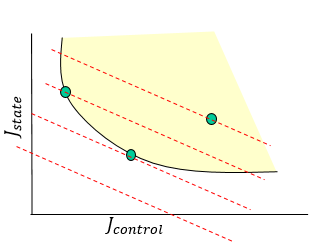
\includegraphics[width=0.5\textwidth]{..\cost-tradeoff.PNG}\\
  \caption{Tradeoff in the cost of state and control}\label{fig:L12-cost-tradeoff}
  \end{centering}
\end{figure}


\paragraph{Movement cost problem}\ \\

Assume we have the following simpler problem. We do not have any
state cost, but we only need to reach a desired final state. The
only cost is over the control $J_{control}=\sum_t \|u_t\|^2$. How
would the solution look like?

To be more concrete, consider the simple dynamics $x_{t+1}=x_t+u_t$,
which implies $A=B=I$. We are given a desired final state
$X_{final}=x_T$ and we like to set the controls.

A naive solution is to set $u_1=x_{final}-x_0$ and $u_t=0$ for
$t\geq 2$. The cost is $\|u_1\|^2=\|x_{final}-x_0\|^2$. The good
news is that it is finite, the bad news is that we can do much
better. Rather than doing the move in a single step, we can do it in
$T$ steps. We set $u_t= \frac{x_{final}-x_0}{T}$, and the cost is
$\sum_t \|u_t\|^2=T\|\frac{x_{final}-x_0}{T}\|^2=
\frac{\|x_{final}-x_0\|^2}{T}$. We gained a factor of $T$.

It is not hard to see that this is the optimal solution. First, any
solution which deviate from the line $x_{final}-x_0$ can be only
improved by projecting the controls to that line. Second, given that
we only make steps on the line, equal size steps will minimize our
costs. Namely, $u_t = \alpha_t (x_{final}-x_0)$ such that
$\alpha_t\geq 0$ and $\sum_t\alpha_t=1$, then the cost is $\sum_t
\alpha_t^2$. This is minimized at $\alpha_t=1/T$.

\subsection{Optimal LQR control}

We will use a dynamic programming approach. For each state $x_t$ we
define the cost-to-go as,
\[
J(u_t, \ldots, u_{T-1},x_t)=\sum_{i=t}^{T-1}x_i^\top Qx_i+u_i^\top R
u_i+ x_T^\top Q_f x_T
\]
Any optimal solution for times $[1,T]$ is also an optimal solution
for any suffix $[t,T]$.

We define the optimal value function $V^*_t(x_t)$ from state $x_t$
at time $t$ until time $T$. Our optimization problem is
\[
V^*_0(x_0)=\min_{u_0, \ldots, u_{T-1}} J(u_0, \ldots, u_{T-1},x_0)
\]
At any time $t$ we have
\[
V^*_t(x_t)=x_t^\top Qx_t +(u_t^*)^\top R u_t^*
+V^*_{t+1}(Ax_t+Bu_t^*)
\]
where
\[
u_t^*= \arg\min_u x_t^\top Qx_t +u^\top R u +V^*_{t+1}(Ax_t+Bu)
\]
We construct the optimal control sequence and value functions by
backward derivation from time $t=T$ to time $t=0$.

The main theorem will show how to compute the optimal controls.
\begin{theorem}
The optimal cost-to-go and optimal control at time $t$ is,
\[
V^*_t(x_t)=x_t^\top P_t x_t \;\;\;\; u_t^*=-K_t x_t
\]
where $P_T=Q_f$ and
\[
P_t=Q+K_t^\top RK_t +(A-BK_t)^\top P_{t+1} (A-BK_t)
\]
\[
K_t = (R+B^\top P_{t+1} B)^{-1}B^\top P_{t+1}A
\]
and $P_t$ is a p.s.d. symmetrix matrix.
\end{theorem}

The theorem has a few interesting implications. Optimal cost-to-go
is a quadratic function of state $x_t^\top P_t x_t$. The optimal
control is linear in state $u_t=-K_t x_t$. (See a numeric example in
the slides.)

\begin{proof}
The proof is by backward induction from $t=T$ to $t=0$. We will also
claim that $P_t$ is symmetric and positive semi-definite.

For the base of the induction, $t=T$, we have $P_T=Q_f$ and
$V^*_T(x_T)=x_T^\top Q_f x_T$. (Clearly, $P_T$ is p.s.d. since $Q_f$
is.)

For the induction step, assume the inductive hypothesis holds for
$t$ and we show it for $t-1$.

We have,
\[
V^*_{t-1}(x_{t-1})=\min_u x_{t-1}^\top Qx_{t-1} +u^\top R u
+V^*_{t}(Ax_{t-1}+Bu)
\]
By the inductive hypothesis $V^*_{t}(Ax_{t-1}+Bu)=(Ax_{t-1}+Bu)^\top
P_t(Ax_{t-1}+Bu)$, and we have
\[
V^*_{t-1}(x_{t-1})=\min_u x_{t-1}^\top Qx_{t-1} +u^\top R u
+(Ax_{t-1}+Bu)^\top P_t(Ax_{t-1}+Bu)
\]
We can now solve for $u$:
\[
\nabla_u V_{t-1}^*(x_{t-1})=2u^\top R+2(Ax_{t-1}+Bu)^\top P_t B=0
\]
which implies that
\[
u_{t-1}^*=-(R+B^\top P_tB)^{-1}B^\top P_t A x_{t-1}=-K_{t-1}x_{t-1}
\]
Since $P_t$ is a p.s.d. matrix,  then $R+B^\top P_t B$ is a p.s.d.
matrix. If $R$ is full rank then we have an inverse.
%
This completes the
part that $u_{t-1}$ is linear in $x_{t-1}$.

We now need to compute the value function.
%
\begin{align*}
V^*_{t-1}(x_{t-1}) =& x_{t-1}^\top Qx_{t-1}+(u^*_{t-1})^\top
Ru^*_{t-1} +(Ax_{t-1}+Bu^*_{t-1})^\top P_t (Ax_{t-1}+Bu^*_{t-1})\\
=&x_{t-1}^\top Qx_{t-1}+(K_{t-1}x_{t-1})^\top
RK_{t-1}x_{t-1} +(Ax_{t-1}-BK_{t-1}x_{t-1})^\top P_t (Ax_{t-1}-BK_{t-1}x_{t-1})\\
=& x_{t-1}^\top \left(Q+K^\top_{t-1}RK_{t-1}+(A-BK_{t-1})^\top P_t
(A-BK_{t-1})\right)x_{t-1}\\
=& x_{t-1}^\top P_{t-1}x_{t-1}
\end{align*}
where $P_{t-1}=Q+K^\top_{t-1}RK_{t-1}+(A-BK_{t-1})^\top P_t
(A-BK_{t-1})$. Since $P_{t-1}$ is the sum of p.s.d. matrices, it is
p.s.d matrix. Since $P_t$ is symmetric, $P_{t-1}$ is also symmetric,
i.e., $P_{t-1}=P^\top_{t-1}$.
\end{proof}


\section{LQR: Discrete time infinite horizon}

Assume that the horizon is $T=\infty$. The value function is,
\[
V_0^*(x_0)=\min_{u_0,\ldots} \sum_{t=0}^\infty x_t^\top Q x_t
+u_t^\top R u_t
\]
where $x_{t+1}=Ax_t+Bu_t$.

First, since we have an infinite sum, we need to ask whether the
costs are finite. In the case that we can reach $x_t=0$, then
afterwards, we have that the costs are zero, so the sum is finite.

Similar to the finite horizon case, we have,
\begin{theorem}
There exists matrices $P$ and $K$ such that the optimal cost-to-go
and optimal control at time $t$ is,
\[
V^*_t(x_t)=x_t^\top P x_t \;\;\;\; u_t^*=-K x_t
\]
\end{theorem}

The Bellman's optimality equation states,
\begin{align*}
V^*(x)=& \min_u  x^\top Qx + u^\top Ru+V^*(Ax+Bu)\\
=& \min_u  x^\top Qx + u^\top Ru+(Ax+Bu)^\top P(A+Bu)
\end{align*}
Minimizing over $u$ we have
\begin{align*}
\nabla_u V^*(x)=&  2 u^\top R+2(Ax+Bu)^\top P=0\\
u^*=& -(R+B^\top PB)^{-1}B^\top PAx=-Kx
\end{align*}

The optimal value function is
\begin{align*}
V^*(x)=& x^\top Px\\
=& x^\top Qx + (u^*)^\top Ru^*+(Ax+Bu^*)^\top P(A+Bu^*)\\
=& x^\top (Q+A^\top P A - A^\top P B(R+B^\top P B)^{-1} B^\top P A)x
\end{align*}

Since this holds for any $x$ we have
\[
P=Q+A^\top P A - A^\top P B(R+B^\top P B)^{-1} B^\top P A
\]
which is called the Algebraic Riccati Equation (ERA).


\section{Controllability}

Controllability, is define as the ability to reach from any initial
state $x_0$ any final state $x_D$, after a large enough time $T$. If
the system is controllable, then there exist a solution to the ARE.

Consider how the system evolves:
\begin{align*}
x_{t+1}=& Ax_t+Bu_t\\
=& A(Ax_{t-1}+Bu_{t-1})+Bu_t\\
=&A^2x_{t-1}+ABu_{t-1}+B_{u_t}\\
=& A^3 x_{t-2}+A^2B u_{t-2}+AB u_{t-1}+Bu_t\\
=&A^{t+1} x_0+\sum_{i=0}^{t} A^i B u _{t-i}
\end{align*}

We can define now a matrix $C$ and vector $U$, where
\[
C=[ B\; AB\; A^2B \cdots A^t B] \;\;\; U=[u_t^\top \;u_{t-1}^\top
\cdots u_0^\top]
\]
and we have
\[
x_{t+1}=A^{t+1}x_0 +CU
\]
Therefore a sufficient condition for controllability is to have $C$
full rank. This will ensure that we can enforce that $x_{t+1}=x_D$
for any $x_D$ (by solving the linear equations).

The next question is how large a $t$  we need? Recall that the
states are $x\in \mathbb{R}^n$. We will claim that $t=n-1$ will be
sufficient.

The Cayley-Hamilton theorem states that for any matrix $A$, we have
that $A^n$ is linearly dependent on $A^i$ for $i<n$. One proof is to
consider the characteristic polynomial $p(\lambda)=det(\lambda I
-A)=\sum_{i=0}^n c_i \lambda^i$, where $c_n=1$. Since setting
$\lambda=A$ we get the zero matrix, which implies that
$A^n=\sum_{i=0}^{n-1}-c_i A^i$.) This implies that a sufficient
condition is that the following matrix is full rank
\[
C=[ B\; AB\; A^2B\; \cdots A^{n-1} B]
\]
This also guarantees that the ARE has a solution. (See the slides
for examples)

\section{LQR: Stability}

Let $P$ be the solution to the ARE. Then $K=(R+B^\top P
B)^{-1}B^\top PA$ and $u^*=-Kx$.

Consider the dynamics of the optimal control.
\begin{align*}
x_{t+1} =& Ax_t + Bu_t\\
=& Ax_t -BKx_t\\
=& (A-BK)x_t\\
=&(A-BK)^{t+1}x_0
\end{align*}

Consider the eigenvalues of the matrix $A-BK$. We can write it as
\[
A-BK=M\Lambda M^{-1}
\]
where $\Lambda$ is a diagonal matrix with the eigenvalues
$\lambda_i$ on the diagonal.

If for every $i$ we have $|\lambda_i|<1$ then the system converges
to zero. In such a case the system is {\em stable} and has a finite
cost.

If there exists an $i$ such that $|\lambda_i|>1$ the system diverges
and is not stable. Also, the system has infinite cost (for any
control).

\section{Extensions to LQR}

We will discuss a few extensions of the basic LQR system.
\begin{enumerate}
\item
Affine system: add a constant vector to the dynamics.
\item
Smoothness: Penalize the change in control, i.e., $u_t-u_{t-1}$.
\item
Noise: allow for Gaussian noise. Called Linear Quadratic Gaussian.
\item
Linear Time Varying (LTV) system, having matrices $A_t$ and
$B_t$.
\item
Non-Linear system: Linearize the system
\end{enumerate}

\subsection{LQR: Affine system}

We define a new dynamics, where there is an additional constant
vector $c\in\mathbb{R}^n$. Namely,
\[
x_{t+1}=Ax_t+Bu_t+c
\]
The cost is as before $x_t^\top Qx_t+u_t^\top Ru_t$.  We an affine
system the control remains linear. One way to show that is to redo
all the math. A simpler option is a reduction.
\[
\begin{bmatrix}
x_{t+1}\\
1
\end{bmatrix}
=\begin{bmatrix}
A&c\\
0&1
\end{bmatrix}
\begin{bmatrix}
x_{t}\\
1
\end{bmatrix}+
\begin{bmatrix}
B\\
0
\end{bmatrix}
u_t
\]
This implies that we have a new state $z_t=\begin{bmatrix}
x_{t}\\
1
\end{bmatrix}$, and the new dynamics become
\[
z_{t+1}=A'z_t+B'u_t
\]
We can now apply everything we know about the LQR. We get that the
optimal control $u^*_t$ is linear in $z_t$ and hence linear in
$x_t$.

\subsection{LQR: Smoothness}

We would like to penalize for changing the control. Let $\Delta
u_t=u_t-u_{t-1}$. Our new cost becomes
\[
x^\top_t Qx_t +u_t^\top R u_t + (\Delta u_t)^\top R' \Delta u_t
\]
and the dynamics remain $x_{t+1}=A x_t + B u_t$.

We can reduce this case also to the standard LQR.
\[
\begin{bmatrix}
x_{t+1}\\
u_t
\end{bmatrix}
=\begin{bmatrix}
A&B\\
0&1
\end{bmatrix}
\begin{bmatrix}
x_{t}\\
u_{t-1}
\end{bmatrix}+
\begin{bmatrix}
B\\
I
\end{bmatrix}
\Delta u_t
\]
This implies that we have a new state $z_t=\begin{bmatrix}
x_{t}\\
u_{t-1}
\end{bmatrix}$, and the new dynamics become
\[
z_{t+1}=A'z_t+B'u_t
\]
and cost $Q'$ and $R'$ where
\[
Q'=\begin{bmatrix}Q & 0\\ 0 & R\end{bmatrix}
\]
and the cost is
\[
\sum_{t=0}^\infty z_t^\top Q'z_t+(\Delta u_t)^\top R' \Delta u_t =
\sum_{t=0}^\infty x_t^\top Qx_t+u_{t-1}^\top R u_{t-1}+(\Delta
u_t)^\top R' \Delta u_t
\]


\subsection{Linear Quadratic Gaussian (LQG)}

We add a Gaussian noise to the dynamics,
\[
x_{t+1}=A x_t + B u_t +w_t
\]
where $w_t \sim N(0,W)$ for a correlation matrix $W\in
\mathbb{R}^{n\times n }$.

We have the same objective, but now we like to minimize the expected
cost. Note that now the expected cost in each time is none zero (due
to the noise).

For a finite horizon we have
\[
V^*_t(x_t)= x_t^\top P_t x_t + m_t
\]

 We will show this by
backward induction on $t$. For $t=T$ we have $V_T^*(x)=x^\top Q_fx$.
Assume it holds for $t$ and we show it for $t-1$.
\[
V^*_{t-1}(x_{t-1})=\min_{u_{t-1}} x_{t-1}^\top Qx_{t-1}+u_{t-1}^\top
Ru_{t-1}+E_{w_t\sim N(0,W)}[V^*_t(Ax_{t-1}+Bu_{t-1}+w_t)]
\]
By the induction hypothesis, we have
\[
E[V^*_t(x_t)]=E[(Ax_{t-1}+Bu_{t-1}+w_t)^\top P_t
(Ax_{t-1}+Bu_{t-1}+w_t)]+m_t
\]
This implies that
\[
V^*_{t-1}(x_{t-1})=\min_{u_{t-1}} x_{t-1}^\top Qx_{t-1}+u_{t-1}^\top
Ru_{t-1}+(Ax_{t-1}+Bu_{t-1})^\top P_t (Ax_{t-1}+Bu_{t-1})+m_{t-1}
\]
where $m_{t-1}=m_t +Tr(WP_t)=m_t +\sum_{i,j} W[i,j]P_t[i,j]$.

Note that the solution to the LQG is identical to that of the LQR.

Solving for the optimal control we have
\begin{align*}
\nabla_{u_{t-1}} V^*_{t-1}(x_{t-1}) =&
2u_{t-1}R+2(Ax_{t-1}+Bu_{t-1})^\top P_t B =0\\
u_{t-1}^*=& -(R+B^\top P_t B)^{-1}B^\top P_t Ax_{t-1}\\
V^*_{t-1}(x_{t-1})=&x_{t-1}^\top P_t x_{t-1} + m_{t-1}
\end{align*}
where $m_{t-1}=Tr(WP_t)+m_t$ and $m_T=0$.

\subsection{Time Varying System}

We assume that $x_{t+1}=A_t x_t +B u_t$. The cost is still $x_t^\top
Qx_t+u_t^\top Ru_t$.

The math is very similar to before and we get
\[
u_t^*=-K_t x_t
\]
and
\[
V^*_t(x_t)=x_t^\top P_t x_t
\]

\subsection{Non-linear system}

Assume a general non-linear dynamics
\[
x_{t+1}=f(x_t,u_t)
\]

Assume that the goal is to stabilize the system at state $x^*$.
Clearly we need a control $u^*$ such that $x^*=f(x^*,u^*)$.

The first step would be linearizing the system around $x^*$. Using
Taylor expansion we have
\[
x_{t+1}\approx f(x^*,u^*)+A(x_t-x^*)+B(u_t-u^*)
\]
where the matrices $A$ and $B$ are the partial derivatives of
$f(x^*,u^*)$ with respect to $x$ and $u$.

We can now reduce the approximate system to LQR. Let the state be
$z_t=x_t-x^*$. Let the control be $v_t=u_t-u^*$. We have that
$z_{t+1}=Az_t + Bu_t$ and the cost is $z_t^\top Qz_t+v_t^\top Rv_t$.
This implies that the optimal control is $v_t = -Kz_t$. By
substituting the values we have $u_{t+1}-u^*=-K(x_{t}-x^*)$, which
becomes,
\[
u_{t+1}=u^*-K(x_t-x^*)
\]

When is such a linearization likely to be successful. We need a good
approximation for both $x^*$ and $u^*$.

\section{System Estimation}

So far we have looked only at planning, given a model find the
optimal policy. What happens when the model is unknown?

We will consider a simple  model based approach. We estimate the
system parameters $A$ and $B$. Given the estimated $A$ and $B$ we
can compute the optimal policy.

We will look at two methods, both involving least squares. The first
is an offline method, using ordinary least squares. The second is an
online method, which is called also recursive least squares.



\subsection{Ordinary Least Squares}

Assume we observe a system trajectory $(x_t,u_t)_{t=0}^T$. The
system dynamics are $x_{t+1}=Ax_t+B u_t$, where the unknowns are $A$
and $B$.

We can solve for the $A$ and $B$ using a least squares method
\[
\min_{A,B} \sum_t \| x_{t+1}-(Ax_t+Bu_t)  \|^2
\]
We can treat this as a regression problem. Define
$M=\begin{bmatrix}A\\ B\end{bmatrix}$ and $z_t =[x_t\; u_t]$ (note
that $z_t$ is a row vector). Set,
\[
Z=\begin{bmatrix}z_0\\ \vdots\\z_{T-1}\end{bmatrix}\;\;\; X=
\begin{bmatrix}x_1\\ \vdots\\x_{T}\end{bmatrix}
\]
We have that $X\approx Z M$. The least square solution is
$\hat{M}=(Z^\top Z)^{-1}Z^\top X$, assuming $Z^\top Z$ is
invertible.

\subsection{Recursive Least Squares}

The idea is to keep continuously updating the matrix $\hat{M}$ as we
get more observations. Let
\[
\hat{M}_t = (Z_t^\top Z_t)^{-1}Z_t^\top X_t=\Phi_t^{-1}\Psi_t
\]
where $\Phi_t=Z_t^\top Z_t=\sum_{i=1}^t z_i^\top z_i$ and
$\Psi_t=Z_t^\top X_t=\sum_{i=1}^t z_i^\top x_i$.

We can now update the parameters as follows:
\begin{align*}
\Phi_{t+1}^{-1}=&(\Phi_t+z_t^\top z_t)^{-1} =
\phi_t^{-1}-\frac{\Phi_t^{-1}z_{t+1}z_{t+1}^\top\Phi_t^{-1}}{1+z_{t+1}^\top\Phi_t^{-1}z_{t+1}}\\
\Psi_{t+1}=&\Psi+z_{t+1}^\top x_{t+1}\\
\hat{M}_{t+1}=&\Phi_{t+1}^{-1}\Psi_{t+1}
\end{align*}



\section{Bibliography Remarks}

The lecture borrows from the scribe note of
\href{https://courses.cs.washington.edu/courses/cse599i/18wi/resources/lecture20/lecture20.pdf}{Kevin
Jamieson}.


The autonomous helicopter is from Abbeel et al. \cite{AbbeelCN2010}

\bibliography{../bib-lecture}
\bibliographystyle{plain}


% \chapter{Inverse RL and Apprenticeship learning}
% \label{chapter:IRL}
% \section{Inverse Reinforcement Learning}

The classical reinforcement problem has as inputs the dynamics and
the rewards and the output is the optimal policy. In the inverse
reinforcement learning problem we are given access to the optimal
policy and the dynamics, and would like to learn a reward function
which induces the given optimal policy.

More specifically, we are given as inputs the states $S$, actions
$A$, dynamics $p(\cdot|s,a)$, and access to the optimal policy
$\pi^*$, either explicitly or implicitly, by observing trajectories
of $\pi^*$.

We have a few related problems:
\begin{enumerate}
\item
Behavioral cloning: given trajectories learn the optimal policy.
\item
Inverse Reinforcement Learning (IRL): which recovers a reward
function $R$ for which $\pi^*$ is optimal.
\item
Apprentice learning: Learn a near-optimal policy given access to
trajectories of an optimal policy.
\end{enumerate}

\subsection{Behavioral Cloning}

Formulated as a classical supervised classification problem. Given
trajectories generated from $\pi^*$, we extract pairs $(s_t,a_t)$,
where $\pi^*(s_t)=a_t$. We do not need to know the dynamics or the
rewards. We define a classification problem, where the training
examples are ${\cal S}=\{(s_t,a_t)\}$.

We can now learn a classifier for ${\cal S}$, and use any
classifier, DNN, SVM, decision tree, and more. We learn the optimal
policy as a classification problem, and if we have low error we can
hope for performance near that of the optimal policy.

There are a few problems with the approach. After we make errors we
might reach completely new states, which we never encountered before
(since the optimal policy never reaches them). Also, the different
errors might have very different effects, but we treat them all
equally. Other issues include generalization, which would depend on
the test and train distributions (of states) being identical, but
small differences in the policies might lead to significant
differences in the distributions.


\subsection{IRL: small state space}

Assume we can use a look-up table to represent the policies. We are
given the set of states $S$, actions $A$, $p(\cdot|s,a)$ and the
optimal policy $\pi^*$. (All are given explicitly, as look-up
tables.) The output of the algorithm is a reward function $r(s,a)$
for which $\pi^*$ is optimal.

We first characterize all the rewards $R$ for which $\pi^*$ is
optimal. Bellman optimality requires that for every $s\in S$ and
$a\in A$ we have,
\[
Q^*(s,\pi^*(s))\geq Q^*(s,a)
\]
First we will try to get a more explicit characterization.

For simplicity of the notation let $a_1=\pi^*(s)$ for every $s\in
S$. (This is simply renaming the actions.) Also, we associate the rewards with states (rater
then state-action pairs). Define matrices $P^a$,
for $a\in A$, as follows: $P^a[i,j]=p(s_j|s_i,a)$, which is the
transition probabilities using action $a$. Since $a_1$ is the
optimal action, we define $P^*=P^{a_1}$.

For the optimal value function $V^*\in \mathbb{R}^{|S|}$ has
\[
V^*=R+\gamma P^*V^*
\]
This implies that $V^*=(I-\gamma P^*)^{-1}R$. (The inverse exists,
since the eigenvalues of $P^*$ are in the unit circle, hence, all
the eigenvalues of $I-\gamma P^*$ are non-zero.)

The optimal state-action function is,
\[
Q^*=R+\gamma P^a V^*=R+\gamma P^a (I-\gamma P^*)^{-1}R
\]
From the Bellman optimality we have $Q^*(s,\pi^*(s))- Q^*(s,a)\geq
0$ which implies,
\[
(P^*-P^a) (I-\gamma P^*)^{-1}R\geq 0
\]

This establishes the following claim:
\begin{claim}
Reward function $R$ is optimal iff $(P^*-P^a) (I-\gamma
P^*)^{-1}R\geq 0$.
\end{claim}

Although we have an exact characterization, we have a few
challenges.
\begin{enumerate}
\item
Trivial solutions: We can simply set $R=0$ and any policy is
optimal!
\item
What happens if we observe only trajectories of $\pi^*$ and not the
explicit policy and dynamics.
\item
Large state space.
\end{enumerate}

To overcome the ambiguity of the reward function we can set an
objective that will force a unique outcome. One solution is a {\em
max margin}, specifically,
\[
\max_{s\in S} \left\{ Q^*(s,a^*)-\max_{a\neq a^*} Q^*(s,a) \right\}
\]
The resulting linear program is,\\
\begin{align*}
&\max \lambda\\
\forall a^*\neq a\;\;\;\; & (P^*-P^a) (I-\gamma P^*)^{-1}R\geq \lambda  \\
&-R_{max}\leq R\leq R_{max}
\end{align*}


\subsection{AL: Linear function approximation}

In this section we consider the case where we are given access to
trajectories of the optimal policy, in a large state space. Our goal
is to find a near optimal policy.
%Since we have a large state space we would use function approximation.
%
We consider a  simple case that the rewards are linear in the state
representation. For each state $s\in S$ we have
$\phi(s)\in\mathbb{R}^n$. There is a reward weights
$w\in\mathbb{R}^n$. The reward in state $s$ is $w^\top \phi(s)$.

Consider the value function of the policy $\pi$.
\begin{align*}
V^*(s_0) =& E[\sum_{t=0}^\infty \gamma^t r_t|\pi]\\
 =& E[\sum_{t=0}^\infty \gamma^t w^\top \phi(s_t)|\pi]\\
 =& w^\top  \sum_{t=0}^\infty \gamma^tE[ \phi(s_t)|\pi]\\
 =& w^\top \mu(\pi)
\end{align*}
where $\mu(\pi)=\sum_{t=0}^\infty \gamma^tE[ \phi(s_t)|\pi]$. Note
that $\mu(\pi)$ depends on the dynamics (steady state distribution)
that policy $\pi$ induces.

For IRL we like to recover a weight vector $w$ such that for any
policy $\pi$ we have,
\[
w^\top \mu(\pi^*)\geq w^\top \mu(\pi)
\]
First, we can approximate $\mu(\pi)$ from sample of $m$
trajectories,
\[
\mu(\pi)\approx \hat{\mu}(\pi)=\frac{1}{m}\sum_{i=1}^m \sum_{t=0}^H
\gamma^t \phi(s_t)
\]
Second, observe that if we have $\|\mu(\pi)-\hat{\mu}(\pi)\|_2\leq
\epsilon$ then for any $w$ we have
\[
|w^\top \mu(\pi)-w^\top\hat{\mu}(\pi)|\leq \epsilon \|w\|_2
\]

For the AL we like to find a near optimal policy $\pi'$, but we do
not have access to the rewards. However, if we find a policy $\pi'$
such that $\mu(\pi')\approx\mu(\pi^*)$, then for any weights $w$ the
policy $\pi'$ will give a similar expected return as $\pi^*$.

Consider first the IRL problem. As before, we have a problem that
$w=0$ is a solution. We will overcome this by defining a max margin
linear program.
\begin{align*}
& \max \lambda\\
\forall \pi\;\;\;\;  &  w^\top \mu(\pi^*) \geq w^\top\mu(\pi) +\lambda \\
& \|w\|_2^2 \leq 1
\end{align*}

A clear weakness is that we have an exponential size linear program.
We will overcome this by an {\em incremental constraint generation}
which will solve the AL. We maintain a set of policies $\Pi$, where
initially $\Pi=\emptyset$. Initially we select some $\pi^0$ and let
$\mu^0=\mu(\pi^0)$. At iteration $i$ we solve
\[
\max_w \min_{\pi_j\in \Pi} w^\top (\mu^*-\mu^j)
\]
If the value is at most $\epsilon$ we terminate. Otherwise let $w^i$
be the maximizer. We solve for the optimal policy $\pi^i$ given
weights $w^i$ and add $\pi^i$ to $\Pi$. At termination, we compute a
$\mu=\sum_{i=1}^k a_i\mu^i$ which minimizes $\|\mu^*-\mu\|_2$, where
$a_i\geq 0$ and $\sum_i a_i=1$.

The correctness of the constraint generation follows from the
following lemma.
\begin{lemma}
At termination $\|\mu^*-\mu\|_2\leq \epsilon$
\end{lemma}
We can implement $\mu$ by selecting policy $\pi^i\in\Pi$  with
probability $a_i$ and running it to completion.

The main issue is the rate of convergence. How long will it take to
terminate. The following lemma guarantees the fast convergence.
\begin{lemma}
The number of iterations is bounded by
\[
O(\frac{n}{(1-\gamma)^2\epsilon^2}\log\frac{n}{(1-\gamma)\epsilon})
\]
\end{lemma}
\section{Bibliography Remarks}

%The trajectory trees for approximate planning and evaluation is
%taken from \cite{KearnsMN99,KearnsMN02}.

The inverse reinforcement learning follows \cite{PieterN04,NgR00}


% \appendix

% \chapter{Dynamic Programming}
% \label{chapter:dp}
% In this book, we focused on Dynamic Programming (DP) for solving problems that involve dynamical systems. The DP approach applies more broadly, and in this chapter we briefly describe DP solutions to computational problems of various forms. An in-depth treatment can be found in Chapter 15 of \cite{BookCormenLRS2009}.

% Some of the problems below are nicely explained in
% \url{https://people.cs.clemson.edu/~bcdean/dp_practice/}

The dynamic programming recipe can be summarized as follows: \textit{solve a large computation problem by breaking it down into sub-problems, such that the optimal solution of each sub-problem can be written as a function of optimal solutions to sub-problems of a smaller size}. The key is to order the computation such that each sub-problem is solved only once.

We remark that in most cases of interest, the recursive structure is not evident or unique, and its proper identification is part of the DP solution. To illustrate this idea, we proceed with several examples.

\subsection*{Fibonacci Sequence}
The Fibonacci sequence is defined by:
\begin{equation*}
    \begin{split}
        \Value_{0} &= 0 \\ 
        \Value_1 &= 1 \\
        \Value_{\ttime} &= \Value_{{\ttime}-2} + \Value_{{\ttime}-1}.
    \end{split}
\end{equation*}
Our `problem' is to calculate the $\tHorizon$'s number in the sequence, $\Value_{\tHorizon}$. Here, the recursive structure is easy to identify from the problem description, and a DP algorithm for computing $\Value_{\tHorizon}$ proceeds as follows:

\begin{enumerate}
    \item Set $\Value_{0} = 0$,$\Value_1 = 1$ 
    \item For $\ttime = 2, \ldots, \tHorizon$, set
    \begin{equation*}
        \Value_{\ttime} = \Value_{{\ttime}-2} + \Value_{{\ttime}-1}.
    \end{equation*}
\end{enumerate}

Our choice of notation here matches the finite horizon DP problems in Chapter \ref{chapter:DDP}: the effective `size' of the problem $\tHorizon$ is similar to the horizon length, and the quantity that we keep track of for each sub-problem $\Value$ is similar to the value function. Note that by ordering the computation in increasing $\ttime$, each element in the sequence is computed \textit{exactly once}, and the complexity of this algorithm is therefore $O(\tHorizon)$.

We will next discuss problems where the DP structure is less obvious.

\subsection*{Maximum Contiguous Sum}
We are given a (long) sequence of $\tHorizon$ real numbers ${x_1},{x_2}, \ldots ,{x_\tHorizon}$, which could be positive or negative. Our goal is to find the maximal contiguous sum, namely,
\[{\Value^*} = \mathop {\max }\limits_{1 \leq \ttime_1 \leq \ttime_2 \le \tHorizon} \;\,\sum\limits_{\ell  = \ttime_1}^{\ttime_2} {{x_\ell }} .\]

An exhaustive search needs to examine $O({\tHorizon^2})$ sums. We will now devise a more efficient DP solution. Let 
\begin{equation*}
    {\Value_{\ttime}} = \mathop {\max }\limits_{1 \le \ttime' \le {\ttime}} \sum\limits_{\ell  = \ttime'}^{\ttime} {{x_\ell }}
\end{equation*}
denote the maximal sum over all contiguous subsequences that end exactly at ${x_{\ttime}}$. We have that:
\begin{equation*}
    \Value_1 = x_1,
\end{equation*}
and
\begin{equation*}
    \Value_{\ttime} = \max \{\Value_{\ttime - 1}+ x_{\ttime}, x_{\ttime} \}.
\end{equation*}
Our DP algorithm thus proceeds as follows:
\begin{enumerate}
    \item Set $\Value_1 = x_1$, $\policy_1 = 1$
    \item For $\ttime = 2, \ldots, \tHorizon$, set
    \begin{equation*}
    \begin{split}
        \Value_{\ttime} &= \max \{\Value_{\ttime - 1}+ x_{\ttime}, x_{\ttime} \}, \\
        \policy_{\ttime} &= \begin{cases}
                                \policy_{\ttime-1}, & \text{if } \Value_{\ttime - 1}+ x_{\ttime} > x_{\ttime} \\
                                \ttime & \text{else. } 
                              \end{cases}
    \end{split}
    \end{equation*}
    \item Set $\ttime^* = \argmax_{1 \leq \ttime \leq \tHorizon} \Value_{\ttime}$
    \item Return $\Value^* = \Value_{\ttime^*}$, $\ttime_{\text{start}}=\policy_{\ttime^*}$, $\ttime_{\text{end}}=\ttime^*$.
\end{enumerate}
This algorithm requires only $O(\tHorizon)$ calculations, i.e., linear time. Note also that in order to return the range of elements that make up the maximal contiguous sum $[\ttime_{\text{start}},\ttime_{\text{end}}]$, we keep track of $\policy_{\ttime}$ -- the index of the first element in the maximal sum that ends exactly at ${x_{\ttime}}$. 

\subsection*{Longest Increasing Subsequence}

We are given a sequence of $\tHorizon$ real numbers ${x_1},{x_2}, \ldots ,{x_{\tHorizon}}$. Our goal is to find the longest strictly increasing subsequence (not necessarily contiguous).
E.g, for the sequence $(3,1,5,3,4)$, the solution is $(1,3,4)$.
Observe that the number of subsequences is ${2^{\tHorizon}}$, therefore an exhaustive search is inefficient.

We next develop a DP solution. Define  ${\Value_{\ttime}}$ to be the length of the longest strictly increasing subsequence ending at position $\ttime$.
Then 
\begin{equation*}
\begin{split}
    {\Value_1} &= 1, \\
    \Value_{\ttime} &= \left\{\begin{array}{ll}
  1, & \text{if } x_{\ttime'}\geq x_{\ttime} \text{ for all } \ttime'<\ttime, \\
  \max \left\{{\value_{\ttime'} : \ttime'<\ttime, x_{\ttime'}<x_{\ttime}}\right\}+1,& \text{else}. \end{array}\right. 
\end{split}
\end{equation*}

The size of the longest subsequence is then $\Value^* = {\max _{1 \le \ttime \le \tHorizon}}({\Value_{\ttime}}).$ 
Computing ${\Value_{\ttime}}$ recursively gives the result with a running time of $O({\tHorizon^2})$.\footnote{We note that this can be further improved to $O(\tHorizon\log \tHorizon)$. See Chapter 15 of
\cite{BookCormenLRS2009}.}


\subsection*{An Integer Knapsack Problem}

We are given a knapsack (bag) of integer capacity $C > 0$, and a set of $\tHorizon$ items with respective sizes ${\state_1}, \ldots ,{\state_{\tHorizon}}$ and values (worth) ${\reward_1}, \ldots ,{\reward_{\tHorizon}}$. The sizes are positive and integer-valued. Our goal is to fill the knapsack to maximize the total value. That is, find the subset $A \subset \{ 1, \ldots ,\tHorizon\} $ of items that maximize \[\sum\nolimits_{\ttime \in A} {{\reward_{\ttime}}} ,\] subject to  \[\sum\nolimits_{\ttime \in A} {{\state_\ttime}}  \le C.\]

Note that the number of item subsets is ${2^\tHorizon}$. We will now devise a DP solution.
Let $\Value(\ttime,\ttime') = $ denote the maximal value for filling exactly capacity $\ttime'$ with items from the set $\{1, \ldots,\ttime\}$.
If the capacity $\ttime'$ cannot be matched by any such subset, set $\Value(\ttime,\ttime') =  - \infty $.
Also set $\Value(0,0) = 0$, and  $\Value(0,\ttime') =  - \infty $ for $\ttime' \ge 1$.  Then
\begin{equation*}
  \Value(\ttime,\ttime') = \max \{ \Value(\ttime - 1,\ttime'), \Value(\ttime - 1,\ttime' - {\state_{\ttime}}) + {\reward_{\ttime}}\},  
\end{equation*}
which can be computed recursively for $\ttime = 1:\tHorizon$,  $\ttime' = 1:C$. The required value is obtained by    $\Value^* = {\max _{0 \le \ttime' \le C}}\Value(\tHorizon,\ttime')$.
The running time of this algorithm is $O(\tHorizon C)$.  We note that the recursive computation of $\Value(\ttime,\ttime')$ requires $O(C)$ space. To obtain the indices of the terms in the optimal subset some additional book-keeping is needed, which requires $O(\tHorizon C)$  space.

\subsection*{Longest Common Subsequence}\label{ss:LCS}
We are given two sequences (or strings) $X(1:\tHorizon_1)$, $Y(1:\tHorizon_2)$, of length $\tHorizon_1$ and $\tHorizon_2$, respectively. We define a \textit{subsequence} of X as the string that remains after deleting some number (zero or more) of elements of X.  We wish to find the longest common subsequence (LCS) of X and Y, namely, a sequence of maximal length that is a subsequence of both X and Y.
For example:
\begin{equation*}
    \begin{split}
       X &= \underline{A}V\underline{B}V\underline{A}M\underline{C}\underline{D}, \\
       Y &= \underline{A}Z\underline{B}Q\underline{A}\underline{C}L\underline{D}.
     \end{split}
\end{equation*}

We next devise a DP solution.
Let  $\Value(\ttime_1,\ttime_2)$ denote the length of an LCS of  the prefix subsequences $X(1:\ttime_1)$, $Y(1:\ttime_2)$. Set $\Value(\ttime_1,\ttime_2) = 0$ if $\ttime_1 = 0$ or $\ttime_2 = 0$. Then, for $\ttime_1,\ttime_2 > 0$, we have:
\begin{equation*}
    \Value(\ttime_1,\ttime_2) = \left\{ {\begin{array}{*{20}{l}}
    {\Value(\ttime_1 - 1,\ttime_2 - 1) + 1}&{\;:\quad X(\ttime_1){\rm{ = }}Y(\ttime_2){\rm{  }}}\\
{\max \{ \Value(\ttime_1,\ttime_2 - 1),\Value(\ttime_1 - 1,\ttime_2)\} }&{\;:\quad X(\ttime_1) \ne Y(\ttime_2)}
\end{array}} \right.
\end{equation*}
We can now compute $\Value(\tHorizon_1, \tHorizon_2)$ recursively, using a row-first or column-first order, in $O(\tHorizon_1 \tHorizon_2)$ computations.

\subsection*{Further examples}
% The references mentioned above provide additional details on these problems, as well as a number of problems. These include, among others:
Additional important DP problems include, among others:
\begin{itemize}
  \item The Edit-Distance problem: find the distance (or similarity) between two strings, by counting the minimal number of ``basic operations'' that are needed to transform one string to another. A common set of basic operations is: delete character, add character, change character. This problem is frequently encountered in natural language processing and bio-informatics (e.g., DNA sequencing) applications, among others.
  \item The Matrix-Chain Multiplication problem: Find the optimal order to compute a matrix multiplication  ${M_1}{M_2} \cdots {M_n}$  (for non-square matrices).
\end{itemize}




\setcounter{chapter}{1}
\chapter{Deterministic Decision Processes}
\label{chapter:DDP}
\input{chapter2-DDP}

\setcounter{chapter}{2}

\chapter{Markov Chains}
\label{chapter:MC}


%\section{Markov Chains}

We start by considering a stochastic dynamics model which does not
have any actions, so that we can concentrate on the dynamics.

A \emph{Markov chain} $\{ {X_\ttime},\;\ttime = 0,1,2, \ldots \} $, with
${X_\ttime} \in X$, is a discrete-time stochastic process, over a
finite or countable state-space $X$, that satisfies the following
Markov property:
    \[{\cal P}({X_{\ttime +1}} = j|{X_\ttime} = i,{X_{\ttime - 1}}, \ldots {X_0}) = {\cal P}({X_{\ttime +1}} = j|{X_\ttime} = i).\]
We focus on time-homogeneous Markov chains, where
\[{\cal P}({X_{\ttime +1}} = j|{X_\ttime} = i) = {\cal P}({X_1} = j|{X_0} = i) \buildrel \Delta \over = {p_{i,j}}.\]
The ${p_{i,j}}$'s  are the transition probabilities, which satisfy
$p_{i,j} \ge 0$, and for each $ i\in X$ we have $\sum_{j \in X}
{{p_{i,j}} = 1} $, namely, $\{p_{i,j}:j\in X\}$ is a distribution on
the next state following state $i$.  The matrix $P = ({p_{i,j}})$ is
the transition matrix. The matrix is row-stochastic (each row sums
to $1$ and all entries non-negative).

Given the initial distribution ${p_0}$ of ${X_0}$, namely ${\cal
P}({X_0} = i) = {p_0}(i)$, we obtain the finite-dimensional
distributions:
\[{\cal P}({X_0} = {i_0}, \ldots ,{X_\ttime} = {i_\ttime}) = {p_0}(i_0){p_{{i_0},{i_1}}} \cdot  \ldots  \cdot {p_{{i_{\ttime - 1}},{i_\ttime}}}.\]

Define $p_{i,j}^{(m)} = {\cal P}({X_m} = j|{X_0} = i),$ the $m$-step
transition probabilities.  It is easy to verify that $p_{i,j}^{(m)}
= {[{P^m}]_{ij}}$  (here ${P^m}$ is the $m$-th power of the matrix
$P$).

\begin{example}
\footnote{Simple MC, two states, running example.} Consider the
following two state Markov chain, with transition probability $P$
and initial distribution $p_0$, as follows:
$$
P=
\begin{pmatrix}
0.4 & 0.6  \\
0.2 & 0.8
\end{pmatrix}
\qquad p_0=
\begin{pmatrix}
0.5  & 0.5
\end{pmatrix}
$$
Initially, we have both states equally likely. After one step, the
distribution of states is $p_1=p_0 P=(0.3\;,\; 0.7)$. After two
steps we have $p_2=p_1 P=p_0 P^2 = (0.26 \;,\; 0.74 )$. The limit of
this sequence would be $p_\infty =(0.25 \;,\; 0.75)$, which is
called the {\em steady state distribution}, and would be discussed
later.
\end{example}

\paragraph{State classification:}

\begin{itemize}
\item State $j$ is \textit{accessible} from $i$  (denoted by $i \to j$) if $p_{i,j}^{(m)} > 0$ for some $m \ge
1$.\\
For a finite $X$  we can compute the accessibility property as
follows. Construct a directed graph $G(X,E)$ where the vertices are
the states $X$ and there is a directed edge $(i,j)$ if $p_{i,j}>0$.
State $j$ is accessible from state $i$ iff there exists a directed
path in $G(X,E)$ from $i$ to $j$.
\item States $i$ and $j$ are \textit{communicating} states (or communicate) if $i \to j$ and $j \to
i$.\\
For a finite $X$, this implies that in $G(X,E)$ there is both a
directed path from $i$ to $j$ and from $j$ to $i$.
\item A \textit{communicating class} (or just
\emph{class}) is a maximal collection of states that communicate.\\
For a finite $X$, this implies that in $G(X,E)$ we have $i$ and $j$
in the same strongly connected component of the graph. (A strongly
connected component has a directed path between any pair of
vertices.)
\item The Markov chain is
\textit{irreducible} if all states belong to a single class (i.e.,
all states communicate with each other).\\
For a finite $X$, this implies that in $G(X,E)$ is strongly
connected.
\item
State $i$ has a \textit{period} $d_i=GCD \{m\geq
1:p_{i,i}^{(m)}>0\}$, where $GCD$ is the greatest common divisor. A
state is aperiodic if $d_i=1$.\\
State $i$ is periodic with period $d_i \ge 2$ if  $p_{i,i}^{(m)} =
0$ for $m \pmod {d_i} \neq 0$ and for any $m$ such that
$p_{i,i}^{(m)} > 0$ we have $m \pmod {d_i} =0$.\\
If a state $i$ is aperiodic, then there exists an integer $m_0$ such
that for any $m\geq m_0$ we have $p_{i,i}^{(m)}>0$.
\item
Periodicity is a class property: all states in the same class
have the same period. Specifically, if some state is
\textit{a-periodic},
then all states in the class are a-periodic.\\
\begin{claim}
For any two states $i$ and $j$ with periods $d_i$ and $d_j$, in the
same communicating class, we have $d_i=d_j$.
\end{claim}
\begin{proof}
For contradiction, assume that $d_j \pmod {d_i}\neq 0$. Since they
are in the same communicating class, we have a trajectory from $i$
to $j$ of length $m_{i,j}$ and from $j$ to $i$ of length $m_{j,i}$.
This implies that $(m_{i,j}+m_{j,i})\pmod {d_i}=0$. Now, there is a
trajectory (which is a cycle) of length $m_{j,j}$ from $j$ back to
$j$ such that $m_{j,j}\pmod {d_i}\neq 0$ (otherwise $d_i$ divides
the period of $j$). Consider the path from $i$ to itself of length
$m_{i,j}+m_{j,j}+m_{j,i}$. We have that $(m_{ij}+m_{jj}+m_{ji})\pmod
{d_i} = m_{jj}\pmod {d_i} \neq 0$. This is a contradiction to the
definition of $d_i$. Therefore, $d_j \pmod {d_i}=0$ and similarly
$d_i \pmod {d_j}=0$, which implies that $d_i=d_j$.
\end{proof}
The claim shows that periodicity is a class property, and all the
states in a class have the same period.
\end{itemize}

\begin{example}
Add figures explaining the definitions.
\end{example}

\paragraph{Recurrence:}
\begin{itemize}
\item
State $i$ is \textit{recurrent} if ${\cal P}({X_\ttime} = i{
\textrm{ for some }}\ttime \ge 1|{X_0} = i) = 1$. Otherwise, state $i$ is
\textit{transient}.\\
%\item
We can relate the state property of recurrent and transient to the
expected number of returns to a state.

\begin{claim}
State $i$ is transient iff $\sum\nolimits_{m = 1}^\infty
{p_{i,i}^{(m)}}  < \infty $.
\end{claim}

\begin{proof}
Assume that state $i$ is transient. Let $q_i={\cal P}({X_\ttime} =
i{ \textrm{ for some }}\ttime \ge 1|{X_0} = i) $. Since state $i$ is
transient we have $q_i<1$. Let $Z_i$ be the number of times the
trajectory returns to state $i$. Note that $Z_i$ is geometrically
distributed with parameter $q_i$, namely $\Pr[Z_i=k]=q_i^k (1-q_i)$.
Therefore the expected number of returns to state $i$ is $1/(1-q_i)$
and is finite.
%
The expected number of returns to state $i$ is equivalently
$\sum\nolimits_{m = 1}^\infty {p_{i,i}^{(m)}} $, and hence if a
state is transient we have $\sum\nolimits_{m = 1}^\infty
{p_{i,i}^{(m)}}  < \infty $.

For the other direction, assume that $\sum\nolimits_{m = 1}^\infty
{p_{i,i}^{(m)}}  < \infty $. This implies that there is an $m_0$
such that $\sum\nolimits_{m = m_0}^\infty {p_{i,i}^{(m)}}  < 1/2$.
Consider the probability of returning to $i$ within $m_0$ stages.
This implies that ${\cal P}({X_\ttime} = i{ \textrm{ for some }}t
\ge m_0|{X_0} = i)< 1/2$. Now consider the probability $q'_i={\cal
P}({X_\ttime} = i{ \textrm{ for some }}m_0\geq \ttime \ge 1|{X_0} = i) $.
%
If $q'_i<1$, this implies that ${\cal P}({X_\ttime} = i{ \textrm{
for some }}\ttime \ge 1|{X_0} = i)<q'_i +(1-q'_i)/2=(1+q'_i)/2<1$, which
implies that state $i$ is transient.
%
If $q'_i=1$, this implies that after at most $m_0$ stages we are
guarantee to return to $i$, hence the expected number of return to
state $i$ is infinite, i.e., $\sum\nolimits_{m = 1}^\infty
{p_{i,i}^{(m)}}  = \infty $. This is in contradiction to the
assumption that $\sum\nolimits_{m = 1}^\infty {p_{i,i}^{(m)}}  <
\infty $.
%This implies that a state is transient iff  the expected number of
%returns to state $i$ is finite and that a state $i$ is recurrent iff
%the expected number of returns to state $i$ is infinite. Since the
%expected number of returns to state $i$ is $\sum\nolimits_{m =
%1}^\infty {p_{i,i}^{(m)}} $, an equivalent criteria is that state
%$i$ is recurrent if and only if $\sum\nolimits_{m = 1}^\infty
%{p_{i,i}^{(m)}}  = \infty $.
\end{proof}


%
%If $\sum\nolimits_{m = 1}^\infty {p_{i,i}^{(m)}}  < \infty $ then
%state $i$ is transient. (By Borel-Cantteli this implies (with
%probability $1$) that such states will only occur a finite number of
%times.)
%
%{\tt The problem is the we cannot use the Borel-Cantteli for the
%other direction, since we needs independence. We still need to show:
%
% State $i$ is
%recurrent if and only if $\sum\nolimits_{m = 1}^\infty
%{p_{i,i}^{(m)}}  = \infty $.
%
%Here is hopefully a correct proof:}
%
%Let $q_i={\cal P}({X_\ttime} = i{ \textrm{ for some }}t \ge 1|{X_0}
%= i) $. Assume that $q_i<1$, i.e., state $i$ is transient. Let $Z_i$
%be the number of times the trajectory returns to state $i$. Note
%that $Z_i$ is geometrically distributed with parameter $q_i$, namely
%$\Pr[Z_i=k]=q_i^k (1-q_i)$. Therefore the expected number of returns
%to state $i$ is $1/(1-q_i)$ and is finite. This implies that a state
%is transient iff  the expected number of returns to state $i$ is
%finite and that a state $i$ is recurrent iff the expected number of
%returns to state $i$ is infinite. Since the expected number of
%returns to state $i$ is $\sum\nolimits_{m = 1}^\infty
%{p_{i,i}^{(m)}} $, an equivalent criteria is that state $i$ is
%recurrent if and only if $\sum\nolimits_{m = 1}^\infty
%{p_{i,i}^{(m)}}  = \infty $.


\item Recurrence is a class property.\\
To see this consider two states $i$ and $j$ such that $j$ is
accessible from $i$ and $i$ is recurrent. Since $i$ is recurrant
$\sum\nolimits_{m = 1}^\infty {p_{i,i}^{(m)}}  = \infty $. Since $j$
is accessible from $i$ there is a $k$ such that $p_{i,j}^{(k)}
>0$. Since $i$ is recurrent, there exists a $k'$ such that
$p_{j,i}^{(k')}>0$. We can lower bound $\sum\nolimits_{m = 1}^\infty
{p_{j,j}^{(m)}}$ by $\sum_{m = 1}^\infty
{p_{j,i}^{(k')}}{p_{i,i}^{(m)}} {p_{i,j}^{(k)}} = \infty $.
Therefore we showed that state $j$ is recurrent.


\item
If states $i$ and $j$ are in the same recurrent (communicating)
class, then state $j$ is (eventually) reached from state $i$ with
probability 1, namely,  ${\cal P}({X_\ttime} = j{\textrm{ for some t}} \ge
1|{X_0} = i) = 1$.\\
This follows from the fact that both states occur infinitely often,
with probability $1$.
\item
Let ${T_i}$ be the {\em return time} to state $i$  (i.e., number of stages
required for $({X_\ttime})$ starting from state $i$ to the first
return to $i$). If $i$ is a recurrent
state, then ${T_i} < \infty $ w.p. 1.\\
Since otherwise, there is a positive probability that we never
return to state $i$, and hence state $i$ is not recurrent.
%
\item State $i$ is {\em positive recurrent} if  $\E({T_i}) < \infty $,
and null recurrent if $\E({T_i}) = \infty $.\\
If the state space $X$
is finite, all recurrent states are positive recurrent.\\
This follows since the set of states that are null recurrent cannot
have transitions from positive recurrent states and cannot have
transition to transient states. If the chain never leaves the set of
null recurrent states, then some state would have a return time
which is at most the size of the set. If there is a positive
probability of leaving the set (and never returning) then the states
are transient. (See the proof of Theorem \ref{thm:countableMC} for a more formal proof of a similar claim for countable Markov Chains.)
\end{itemize}

In the following we illustrate some of the notions that we define. we start with the classic random walk on the integers, where all integer (states) are null recurrent.

\begin{example}{\bf Random walk}
Consider the following Markov chain over the integers. The states
are the integers. The initial states is $0$. At each state $i$, with
probability $1/2$ we move to $i+1$ and with probability $1/2$ to
$i-1$. Namely, $p_{i,i+1}=1/2$, $p_{i,i-1}=1/2$, and $p_{i,j} =0$
for $j \not\in \{i-1,i+ 1\}$. We will show that $T_i$ is finite with
probability $1$ and $\E[T_i]=\infty$. This implies that all the
states are null recurrent.

To compute $\E[T_i]$ consider what happens in one and two steps. Let
$Z_{i,i-1}$ be the time to move from $i$ to $i-1$. Note that  we
have \[
\E[T_i]=1+0.5\E[Z_{i+1,i}]+0.5\E[Z_{i-1,i}]=1+\E[Z_{1,0}],
\]
since, due to symmetry, $\E[Z_{i,i+1}]=\E[Z_{i+1,i}]=\E[Z_{1,0}]$.

In two steps we are either back to $i$, or at state $i+2$ or $i-2$.
For $\E[T_i]$ we have that
\begin{align*}
\E[T_i]=&
2+\frac{1}{4}\E[Z_{i+2,i}]+\frac{1}{4}\E[Z_{i-2,i}] \\
=&2+\frac{1}{4} (\E[Z_{i+2,i+1}]+\E[Z_{i+1,i}])+\frac{1}{4}( \E[Z_{i-2,i-1}]+\E[Z_{i-1,i}])\\
 =&2+E[Z_{1,0}]\\
\end{align*}

This implies that we have
\[
\E[T_i]=1+\E[Z_{1,0}]=2+E[Z_{1,0}]
\]
Clearly, there is no finite value for $\E[Z_{1,0}]$ which will
satisfy the equation, which implies $\E[Z_{1,0}]=\infty$, and hence
$\E[T_i]=\infty$.

To show that state $0$ is a recurrent state, note that the probability
that at time $2k$ we are at state $0$ is exactly $p_{0,0}^{(2k)}={2k
\choose k}2^{-2k}\approx \frac{c}{\sqrt{k}}$, for some $c>0$. This
implies that
$$
\sum\nolimits_{m = 1}^\infty {p_{0,0}^{(m)}}\approx \sum\nolimits_{m
= 1}^\infty \frac{c}{\sqrt{m}}=\infty
$$
and therefore state $0$ is recurrent. (By symmetry, this shows that
all the states are recurrent.)

Note that this Markov chain has a period of $2$. This follows since any trajectory starting at $0$ and returning to $0$ has an equal number of $+1$ and $-1$ and therefore of even length. Any even number $n$ has a trajectory of this length that starts at $0$ and returns to $0$, for example, having $n/2$ times $+1$ followed by $n/2$ times $-1$.
\end{example}

The next example is a simple modification of the random walk, where each time we either return to the origin or continue to the next integer with equal probability. 
This Markov chain will have all (non-negative) integers as possitive recurrent states.

\begin{example}
{\bf Random walk with jumps.}
%
Consider the following Markov chain over the integers. The states
are the integers. The initial states is $0$. At each state $i$, with
probability $1/2$ we move to $i+1$ and with probability $1/2$ we
return to $0$. Namely, $p_{i,i+1}=1/2$, $p_{i,0}=1/2$, and $p_{i,j}
=0$ for $j \not\in \{0,i+ 1\}$. We will show that $\E[T_i]<\infty$
(which implies that $T_i$ is finite with probability $1$).

From any state we return to $0$ with probability $1/2$, therefore
$\E[T_0]=3$. (The expected return is composed from the first move from $0$ to $1$ and then we have a geometric distribution with expectation $2$.) We will show that for state $i$ we have
$\E[T_i]\leq3+3\cdot 2^{i-1}$. We will decompose $T_i$ to two parts. The
first is the return to $0$, this part has expectation $3$. The
second is to reach state $i$ from state $0$. Consider an epoch as
the time between two visits to $0$. The probability that an epoch
would reach $i$ is exactly $2^{-(i-1)}$. The expected time of an epoch
is $3$ (the expected time to return to state $0$). The expected time
to return to state $0$, given that we did not reach state $i$ is
less than $3$. Therefore, $\E[T_i]\leq 3+3\cdot 2^{i-1}$.

Note that this Markov chain is aperiodic.
\end{example}



\paragraph{Invariant Distribution:} %changed pi to mu since pi is latter a policy!
The probability vector $\mu  = ({\mu_i})$ is an invariant
distribution (or stationary distribution or steady state
distribution) for the Markov chain if $\mu^\top P = \mu^\top$,
namely
\[{\mu_j} = \sum_i {{\mu_i}} {p_{i,j}}\quad \forall j.\]
Clearly, if ${X_\ttime} \sim \mu $ then ${X_{\ttime + 1}} \sim \mu
$. If ${X_0} \sim \mu $, then the Markov chain $({X_\ttime})$ is a
stationary stochastic process.


\begin{theorem}
\label{Thm:MC-stationary}
 Let $({X_\ttime})$ be an irreducible and
a-periodic Markov chain over a finite state space $X$ with
transition matrix $P$. Then there is a unique distribution $\mu$
such that $\mu^\top P = \mu^\top >0$.
\end{theorem}

\begin{proof}
Assume that $x$ is an eigenvector of $P$ with eigenvalue $\lambda$,
i.e., we have $Px=\lambda x$. Since $P$ is a stochastic matrix, we
have $\|P x\|_\infty \leq \|x\|_\infty$, which implies that $\lambda
\leq 1$. Since the matrix $P$ is row stochastic, $P\vec{1}=\vec{1}$,
which implies that $P$ has a right eigenvalue of $1$ and this is the
maximal eigenvalue. Since the set of right and left eignevalues is
identical, we conclude that there is $x$ such that $x^\top P=x^\top$.
Our first task is to show that there is such an $x$ with $x\geq0$.

Since the Markov chain is irreducible and a-periodic, there is an
integer $m$, such that $P^m$ has all the entries strictly positive.
Namely, for any $i,j\in X$ we have $p^{(m)}_{i,j}>0$.
%(Formally,

We now show a general property of positive matrices (matrices where
are the entries are strictly positive). Let $A=P^m$ be a positive
matrix and $x$ an eigenvector of $A$ with eigenvalue $1$. First, if
$x$ has complex number then $Re(x)$ and $Im(x)$ are an eigenvectors
of $A$ of eigenvalue $1$ and one of them is non-zero. Therefore we
can assume that $x\in \reals^d$. We would like to show that there is
an $x\geq 0$ such that $x^\top A=x^\top$. If $x\geq 0$ we are done.
If $x\leq 0$ we can take $x'=-x$ and we are done. We need to show
that $x$ cannot have both positive and negative entries.

For contradiction, assume that we have $x_{k}>0$ and $x_{k'}<0$.
This implies that for any weight vector $w>0$ we have $|x^\top w| <
|x|^\top w$, where $|x|$ is point-wise absolute value. Therefore,
\[
\sum_j |x_j|= \sum_j |\sum_i x_i P_{i,j}| < \sum_j \sum_i |x_i|
P_{i,j}=  \sum_i |x_i| \sum_j P_{i,j}= \sum_j |x_j|
\]
where the first identity follows since $x$ is an eigenvector. The
second since $P$ is strictly positive.The third is a change of order
of summation. The last follows since $P$ is a row stochastic matrix, so
each row sums to $1$. Clearly, we reached an contradiction, and
therefore $x$ cannot have both positive and negative entries.

%{\tt [YM:old] To conclude the proof we will show a general property
%of positive matrices (matrices where are the entries are strictly
%positive). Let $A=P^m$ be a positive matrix and $x$ an eigenvector
%of $A$ with eigenvalue $1$, then $|x|$ is an eigenvector of $A$ with
%eigenvalue $1$. (By $|x|$ we mean point-wise absolute value,
%including when the entries are complex numbers.)
%
% Since $x^\top A =x$, then $|x|=|x^\top A|\leq |x|^\top
%A$, where the last inequality is since $A$ is a positive matrix. It
%remains to show that $|x| = |x|^\top A$. Let $z=|x|^\top A$ and
%$y=z-|x|$. We know that $y\geq 0$. Assume that some $y_i>0$. Then
%$y^\top A>0$ since $A$ is a positive matrix and similarly $z>0$.
%
%Now there is an $\epsilon >0$ such that $y^\top A > \epsilon z$,
%which implies that $z^\top B >z$, where $B=\frac{A}{1+\epsilon}$.
%Since the largest eigenvalue of $B$ is $1/(1+\epsilon)<1$, we have
%that the limit $z^\top B^k =0$, which implies that $z<0$. However,
%we established the fact that $z>0$. Therefore, there is no such
%$y_i$, and $|x|$ is an eigenvector of $A$ of eigenvalue $1$. }

We have shown so far that there exists a $\mu$ such that $\mu^\top
P=\mu^\top$ and $\mu\geq 0$. This implies that $\mu/\|\mu\|_1$ is a steady state distribution.
Since $A=P^m$ is strictly positive,
then $\mu^\top=\mu^\top A >0$.

To show the uniqueness of $\mu$, assume we have $x$ and $y$ such
that $x^\top P=x^\top$ and $y^\top P=y^\top$ and $x\neq y$. Recall
that we showed that in such a case both $x>0$ and $y>0$. Then there
is a linear combination $z=ax+by$ such that for some $i$ we have
$z_i=0$. Since $z^\top P=z^\top$, we have showed that $z$ is
strictly positive, i.e., $z>0$, which is a contradiction. Therefore,
$x=y$, and hence $\mu$ is unique.
\end{proof}

We define the average fraction that a state $j\in X$ occurs, given
that we start with an initial state distribution $x_0$,  as follows:
\[
\pi^{(m)}_j=\frac{1}{m}\sum_{t=1}^m \I (X_t=j)
\]

\begin{theorem}
Let $({X_\ttime})$ be an irreducible and  a-periodic Markov chain
over a finite state space $X$ with transition matrix $P$. Let $\mu$
be the stationary distribution of $P$. Then, for any $j\in X$ we
have
\[
\mu_j=\lim_{m\rightarrow\infty} \E[\pi^{(m)}_j] =\frac{1}{\E[T_j]}
\]
\end{theorem}

\begin{proof}
We have that
\[
\E[\pi^{(m)}_j]=\E[\frac{1}{m}\sum_{t=1}^m \I
(X_t=j)]=\frac{1}{m}\sum_{t=1}^m \Pr
[X_t=j|X_0=x_0]=\frac{1}{m}\sum_{t=1}^m x_0^\top P^t
\]
Let $v_1, \ldots , v_n$ be the eigenvectors of $P$ with eigenvalues
$\lambda_1 \geq  \ldots \geq  \lambda_n$. By
Theorem~\ref{Thm:MC-stationary} we have that $v_1=\mu$, the stationary
distribution and $\lambda_1=1>\lambda_i$ for $i\geq 2$. Rewrite
$x_0=\sum_i \alpha_i v_i$. Since $P^m$ is a stochastic matrix,
$x_0^\top P^m$ is a distribution, and therefore $\lim_{m\rightarrow
\infty} x_0^\top P^m=\mu$.
%We claim that $\alpha_1=1$.
%However, for any $v_i$ we have $v_i P^m \rightarrow 0$.

We will be interested in the limit $\pi_j=\lim_{m\rightarrow \infty}
\pi^{m}_j $, and mainly in the expected value $\E[\pi_j]$. From the
above we have that $\E[\pi_j]=\mu_j$.

A different way to express $\E[\pi_j]$ is using a variable time
horizon, with a fixed number of occurrences of $j$. Let $T_{k,j}$ be
the time between the $k$ and $k+1$ occurrence of state $j$. This
implies that
\[
\lim_{m\rightarrow\infty}\frac{1}{m}\sum_{t=1}^m \I (X_t=j) =
\lim_{n\rightarrow\infty} \frac{n}{\sum_{k=1}^n T_{k,j}}
\]
Note that the $T_{k,j}$ are i.i.d. and equivalent to $T_j$. By the
law of large numbers we have that $\frac{1}{n}\sum_{k=1}^n T_{k,j}$
converges to $\E[T_i]$. Therefore,
\[
\E[\pi_j]=\frac{1}{\E[T_j]}
\]
\end{proof}

We have established the following general theorem.

\begin{theorem}[\textbf{Recurrence of finite Markov chains}]
Let $({X_\ttime})$ be an irreducible,  a-periodic Markov chain over
a finite state space $X$.  Then the following properties hold:
\begin{enumerate}
\item All states are \textbf{positive recurrent}
\item There exists a \textbf{unique stationary distribution}
${\mu^*}$, where $\mu^*(i)=1/\E[T_i]$.
\item \textbf{Convergence} to the stationary distribution: ${\lim _{t \to \infty }}p_{i,j}^{(t)} = {\mu_j}\quad (\forall j)$
\item \textbf{Ergodicity}: For any finite $f$: ${\lim _{t \to \infty }}\frac{1}{t}\sum\nolimits_{s = 0}^{\ttime - 1} {f({X_s}) = \sum\nolimits_i {\mu_i f(i) \buildrel \Delta \over = } } \,\pi  \cdot f.$
\end{enumerate}
\end{theorem}

%\begin{proof}
%Item (1): It cannot be that all the states are transient, since then
%all the states will appear only a finite number of times, while the
%run is unbounded. This implies that all the states are recurrent.
%[Need to show {\em positive recurrent}: $\E[T_i]<\infty$]
%
%%Since the Markov chain is irreducible and a-periodic,
%
%Item (2): We will show that for each state $i$ we have
%$\mu^*(i)=1/\E[T_i]$. Let $Z_{i,k}$ be the time from the $k-1$ time
%
%Item (3):
%
%Item (4):
%\end{proof}

For countable Markov chains, there are other possibilities.

\begin{theorem}[\textbf{Countable Markov chains}]
\label{thm:countableMC}
Let $({X_\ttime})$ be an irreducible and a-periodic Markov chain
over a countable state space $X$.  Then:
%\begin{enumerate}
%\item
Either (i) all states are positive recurrent, or (ii) all states are null recurrent, or (iii) all states are transient.
%\item If (i) holds, then properties (2)-(4) of the previous Theorem hold as well.
%\item Conversely, if there exists a stationary distribution $\mu $ then properties (1)-(4) are satisfied.
%\end{enumerate}
\end{theorem}


\begin{proof}
%Item (1):
Let $i$ is a positive recurrent state, then we will show that all
states are positive recurrent. For any state $j$, since the Markov
chain is irreducible, we have for some $m_1,m_2\geq 0$ that
$p^{(m_1)}_{j,i},p^{(m_2)}_{i,j}>0$. This implies that
the return
time to state $j$ is at most $\E[T_j]\leq
1/p^{(m_1)}_{j,i}+\E[T_i]+1/p^{(m_2)}_{i,j}$, and hence $j$ is
positive recurrent.

If there is no positive recurrent state, let $i$ be a null recurrent
state, then we will show that all states are null recurrent. For any
state $j$, since the Markov chain is irreducible, we have for some
$m_1,m_2\geq 0$ that $p^{(m_1)}_{j,i},p^{(m_2)}_{i,j}>0$. This implies that  $\sum_{m=0}^\infty p^{(m)}_{j,j}=\infty$
%
%the probability to return time to state $j$ 
%
is at least
$\sum_{m=0}^\infty
p^{(m_1)}_{j,i}\;p^{(m)}_{i,i}\;p^{(m_2)}_{i,j}=\infty$, since we
have $\sum_{m=0}^\infty p^{(m)}_{i,i}=\infty$, since $i$ is a
recurrent state. This implies that $j$ is a recurrent state. Since
there are no positive recurrent states, it has to be that $j$ is a
null recurrent state.

If there are no positive or null recurrent states, then all states
are transient.
%
%Item (2):
%
%Item (3):
%
\end{proof}

%\begin{leftbar}
\paragraph{Reversible Markov chains:} Suppose there exists a probability vector $\mu  = ({\mu_i})$ so that
\begin{equation}\label{eq:DB}
{\mu _i}{p_{i,j}} = {\mu _j}{p_{j,i}},\quad \quad i,j \in X.
\end{equation}
It is then easy to verify by direct summation that $\mu $ is an
invariant distribution for the Markov chain defined by
$({p_{i,j}})$. This follows since $\sum_i \mu_i p_{i,j}=\sum_i
p_{i,j}\mu_j=\mu_j$. The equations \eqref{eq:DB} are called the
\emph{detailed balance equations}. A Markov chain that satisfies
these equations is called \emph{reversible}.

\begin{example}[\textbf{Discrete-time queue}] Consider a discrete-time queue, with queue length $X_\ttime\in \mathbb{N}_0=\{0,1,2,\dots\}$. At time instant $\ttime$, ${A_\ttime}$ new jobs arrive, and then up to ${S_\ttime}$ jobs can be served, so that
\[{X_{\ttime +1}} = {({X_\ttime} + {A_\ttime} - {S_\ttime})^ + }.\]
Suppose that $({S_\ttime})$ is a sequence of i.i.d. RVs, and
similarly $({A_\ttime})$ is a sequence of i.i.d. RVs, with
$({S_\ttime})$, $({A_\ttime})$ and ${X_0}$ mutually independent. It
may then be seen that $({X_\ttime},\;\ttime \ge 0)$ is a Markov chain.
Suppose further that each ${S_\ttime}$ is a Bernoulli RV with
parameter $q$, namely $P({S_\ttime} = 1) = q$, $P({S_\ttime} = 0) =
1 - q$. Similarly, let ${A_\ttime}$ be a Bernoulli RV with parameter
$p$. Then
\[{p_{i,j}} = \left\{ {\begin{array}{*{20}{l}}
{p(1 - q)}&:&{j = i + 1}\\
{(1 - p)(1 - q) + pq}&:&{j = i,\;\;i > 0}\\
{(1 - p)q}&:&{j = i - 1,\;\;i > 0}\\
{(1 - p) + pq}&:&{j = i = 0}\\
0&:&{{\rm{otherwise}}}
\end{array}} \right.\]
%YM: Need to change mu to eta since mu is the steady state
 Denote $\lambda  = p(1 - q)$, $\eta  = (1 - p)q$, and $\rho  = \lambda /\eta $.   The detailed balance equations for this case are:
\[
\mu_i p_{i,i+1}={\mu _i}\lambda  = {\mu _{i + 1}}\eta=\mu_{i+1}p_{i+1,i} ,\quad \quad \forall i \ge 0\]
These equations have a solution with $\sum {_i{\mu _i} = 1}$ if and
only if $\rho  < 1$. The solution is ${\mu _i} = {\mu _0}{\rho ^i}$,
with ${\pi _0} = 1 - \rho $. This is therefore the stationary
distribution of this queue.
\end{example}
%\end{leftbar}


\paragraph{Mixing time:} %Add definition and motivation
The mixing time measures how fast does the Markov chain converges to the steady state distribution. We first define the Total Variation distance between distributions $D_1$ and $D_2$ is:
\[
\|D_1-D_2\|_{TV}=\sum_{x\in X} | D_1 (x) - D_2(x) |
\]
The mixing time $\tau$ is define as the time to reach a total variation of at most $1/4$:
\[
\|p^{(\tau)}-\mu\|_{TV}\leq 1/4
\]
where $\mu$ is the steady state distribution and $p^{(\tau)}$ is the state distribution after $\tau$ steps.


\chapter{Markov Decision Processes and Finite Horizon}
\label{chapter:MDP-FH}

In  Chapter \ref{chapter:DDP} we considered multi-stage decision
problems for \emph{deterministic} systems. In many problems of
interest, the system dynamics also involves \emph{randomness}, which
leads us to stochastic decision problems. In this chapter we
introduce the basic model of Markov Decision Processes (MDP), which
will be considered in the rest of the book, and discuss the finite
horizon return.



\section{Controlled Markov Chains}

A Markov Decision Process consists of two main parts:
\begin{enumerate}
  \item A controlled dynamic system, with stochastic evolution.
  \item A performance objective to be optimized.
\end{enumerate}
In this section we describe the first part, which is modeled as a controlled Markov chain.

Consider a controlled dynamic system, defined over:
\begin{itemize}
  \item A discrete time axis ${\mathbb{T}} = \{ 0,1, \ldots ,\tHorizon - 1\} $  (finite horizon), or
  ${\mathbb{T}} = \{ 0,1,2, \ldots \} $ (infinite horizon).
To simplify the discussion we refer below to the infinite horizon
case, which can always be ``truncated" at $\tHorizon$ if needed.
  \item A finite state space $\States$, where ${\States_\ttime} \subset \States$ is the set of possible states at time $\ttime\in {\mathbb{T}}$.
  \item A finite action set $\Actions$, where ${\Actions_\ttime}(\state) \subset \Actions$ is the set of possible actions at time $\ttime\in {\mathbb{T}}$ and state $\state \in {\States_\ttime}$.
\end{itemize}

\paragraph{State transition probabilities:}
\begin{itemize}
\item   Suppose that at time $\ttime$ we are in state ${\state_\ttime} = \state$, and choose an action ${\action_\ttime} = \action$. The next state ${\state_{\ttime + 1}} = \state'$ is then determined randomly according to a probability distribution  ${p_\ttime}( \cdot |\state,\action)$ on ${\States_{\ttime + 1}}$. That is,
\[\Pr({\state_{\ttime + 1}} = \state'|{\state_\ttime} = \state,{\action_\ttime} = \action) = {p_\ttime}(\state'|\state,\action),\quad      \quad \state' \in {\States_{\ttime + 1}}\]
\item   The probability ${p_\ttime}(\state'|\state,\action)$ is the \emph{transition probability} from state $\state$ to state $\state'$ for a given action $\action$. We naturally require that
            ${p_\ttime}(\state'|\state,\action) \ge 0$, and $\sum\nolimits_{\state' \in {\States_{\ttime + 1}}}^{} {{p_\ttime}(\state'|\state,\action)}  = 1$ for all $\state \in {\States_\ttime},\action \in {\Actions_\ttime}(\state)$.
\item   Implicit in this definition is the controlled-Markov property:
\[
\Pr({\state_{\ttime + 1}} =
\state'|{\state_\ttime},{\action_\ttime}, \ldots
,{\state_{0,}}{\action_0}) =\Pr({\state_{\ttime + 1}} =
\state'|{\state_\ttime},{\action_\ttime})
\]
\item   The set of probability distributions
                                \[P = \{ {p_\ttime}( \cdot |\state,\action)\;\;:\;\;\state \in {\States_\ttime},\action \in {\Actions_\ttime}(\state),\ttime \in {\T}\} \]
is called the \emph{transition law} or \emph{transition kernel} of the controlled Markov process.
\end{itemize}

\paragraph{Stationary Models:}
    The controlled Markov chain is called stationary or time-invariant if the transition probabilities do not depend on the time $\ttime$. That is:
                     \[\forall t,\quad {p_\ttime}(\state'|\state,\action) \equiv p(\state'|\state,\action),\;\;{\States_\ttime} \equiv \States,\;\;{\Actions_\ttime}(\state) \equiv \Actions(\state).\]

\paragraph{Graphical Notation:}
The state transition probabilities of a Markov chain are often illustrated via a state transition diagram, such as in Figure \ref{fig:MC}.

\begin{figure}
  % Requires \usepackage{graphicx}
  \begin{centering}
  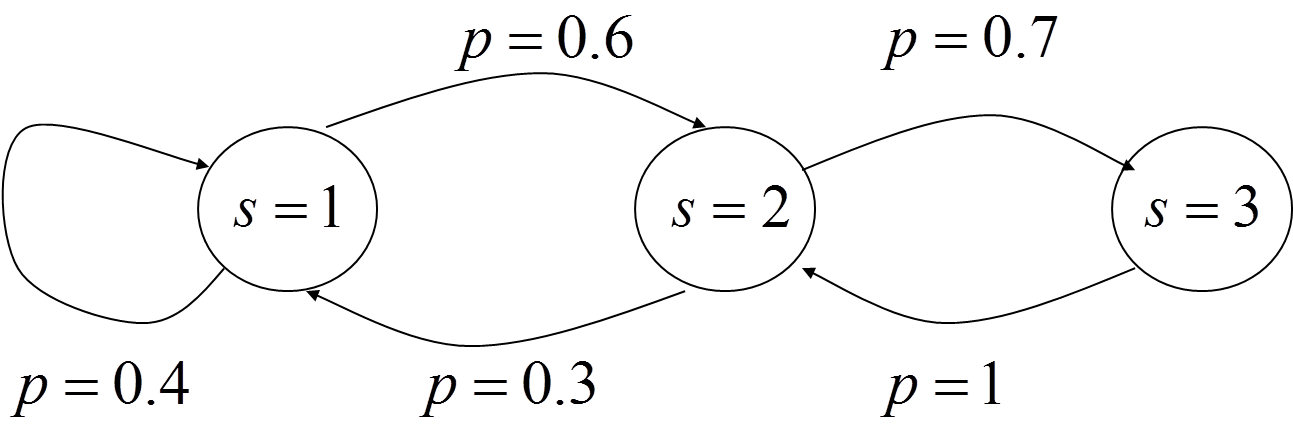
\includegraphics[width=0.7\textwidth]{figures/lecture4_a}\\
  \caption{Markov chain}\label{fig:MC}
  \end{centering}
\end{figure}

A graphical description of a controlled Markov chain is a bit more
complicated because of the additional action variable. We obtain the
diagram (drawn for state $\state = 1$ only, and for a given time
$\ttime$) in Figure \ref{fig:MDP}, reflecting the following
transition probabilities:
\[\begin{array}{l}
p(\state' = 2|\state = 1,\action = 1) = 1\\
p(\state'|\state = 1,\action = 2) = \left\{ {\begin{array}{*{20}{c}}
{0.3}&:&{\state' = 1}\\
{0.2}&:&{\state' = 2}\\
{0.5}&:&{\state' = 3}
\end{array}} \right.
\end{array}\]

\begin{figure}
  % Requires \usepackage{graphicx}
  \begin{centering}
  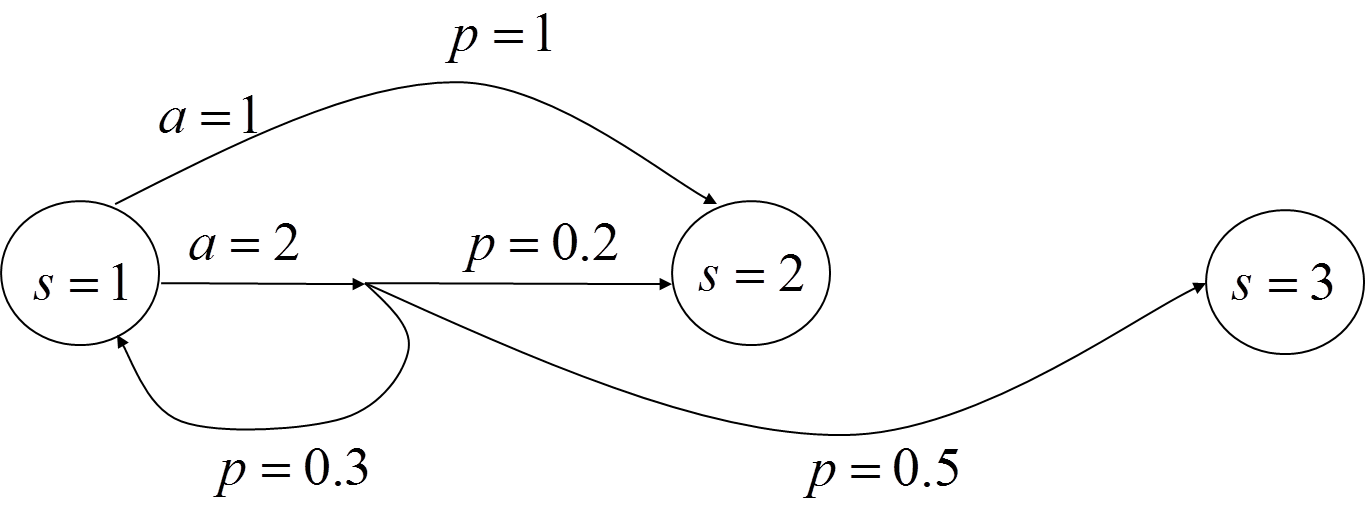
\includegraphics[width=0.7\textwidth]{figures/lecture4_b}\\
  \caption{Controlled Markov chain}\label{fig:MDP}
  \end{centering}
\end{figure}


\paragraph{State-equation notation:}
The stochastic state dynamics can be equivalently defined in terms of a state equation of the form
                                                   \[{\state_{\ttime + 1}} = {f_\ttime}({\state_\ttime},{\action_\ttime},{w_\ttime}),\]
where ${w_\ttime}$ is a random variable (RV).
    If  ${({w_\ttime})_{\ttime \ge 0}}$ is a sequence of independent RVs, and further each ${w_\ttime}$ is independent of the ``past"  $({\state_{\ttime - 1}},{\action_{\ttime - 1}}, \ldots {\state_0})$, then ${({\state_\ttime},{\action_\ttime})_{\ttime \ge 0}}$ is a controlled Markov process.
    For example, the state transition law of the last example can be written in this way, using
                  ${w_\ttime} \in \{ 4,5,6\} $,  with  ${p_w}(4) = 0.3,\;{p_w}(5) = 0.2,\;{p_w}(6) = 0.5$
and, for ${\state_\ttime} = 1$:
    \[\begin{array}{l}
    {f_\ttime}(1,1,{w_\ttime}) = 2\\
    {f_\ttime}(1,2,{w_\ttime}) = {w_\ttime} - 3
    \end{array}\]
  This state algebraic equation notation is especially useful for problems with continuous state space, but also for some models with discrete states.
Equivalently, we can write
    \[
 {f_\ttime}(1,2,{w_\ttime}) = 1\cdot \I[{w_\ttime}=4]+2\cdot \I[{w_\ttime}=5]+3\cdot \I[{w_\ttime}=6] ,
    \]
where $\I[\cdot]$ is the indicator function.

Next we recall the definitions of control policies from Chapter \ref{chapter:DDP}.

\paragraph{Control Policies}
\begin{itemize}
  \item
A general or \textbf{history-dependent deterministic} control policy
$\policy  = {({\policy _\ttime})_{\ttime \in {\mathbb{T}}}}$ is a
mapping from each possible history ${\history_\ttime} =
({\state_0},{\action_0}, \ldots ,{\state_{\ttime -
1}},{\action_{\ttime - 1}},{\state_\ttime})$, and time $\ttime \in
\T$, to an action ${\action_\ttime} = {\policy
_\ttime}({\history_\ttime}) \in {\Actions_\ttime}$.  We denote the
set of general policies by ${\Pi _{HD}}$.
  \item
A \textbf{Markov deterministic} control policy $\policy $ is allowed
to depend on the current state and time only, i.e., ${\action_\ttime} =
{\policy _\ttime}({\state_\ttime})$.   We denote the set of Markov
deterministic policies by ${\Pi _{MD}}$.
  \item
For stationary models, we may define \textbf{stationary
deterministic} control policies that depend on the current state
alone. A stationary policy is defined by a single mapping $\policy
:\States \to \Actions$, so that  ${\action_\ttime} = \policy
({\state_\ttime})$ for all $\ttime \in {\T}$. We denote the set of
stationary policies by ${\Pi _{SD}}$.
  \item Evidently, ${\Pi_{HD}} \supset {\Pi_{MD}} \supset {\Pi_{SD}}$.
\end{itemize}

\paragraph{Randomized Control policies}
\begin{itemize}
  \item The control policies defined above specify deterministically the action to be taken at each stage. In some cases we want to allow for a random choice of action.
  \item A general randomized control policy assigns to each possible history ${\history_\ttime}$ a probability distribution ${\policy _\ttime}( \cdot |{\history_\ttime})$ over the action set ${\Actions_\ttime}$.
  That is,  $\Pr( {\action_\ttime} = \action|{\history_\ttime})  = {\policy _\ttime}(\action|{\history_\ttime})$. We denote the set of history-dependent stochastic policies by ${\Pi _{HS}}$.
  \item Similarly, we can define the set ${\Pi _{MS}}$ of Markov stochastic control policies, where ${\policy _\ttime}( \cdot |{\history_\ttime})$ is replaced by ${\policy _\ttime}( \cdot |{\state_\ttime})$, and the set ${\Pi _{SS}}$ of stationary stochastic control policies, where ${\policy _\ttime}( \cdot |{\state_\ttime})$ is replaced by  $\policy ( \cdot
  |{\state_\ttime})$, namely the policy is independent of the time.
  \item Note that the set ${\Pi _{HS}}$ includes all other policy sets as special cases.
\end{itemize}

\paragraph{The Induced Stochastic Process}
Let  ${p_0} = \{ {p_0}(\state),\state \in {\States_0}\} $ be a
probability distribution for the initial state ${\state_0}$. (Many
times we will assume that the initial state is deterministic and
given by $\state_0$.) A control policy $\policy \in {\Pi _{HS}}$,
together with the transition law $P = \{
{p_\ttime}(\state'|\state,\action)\} $ and the initial state
distribution ${p_0} = ({p_0}(\state),\;\state \in {\States_0})$,
induces a probability distribution over any finite state-action
sequence ${\history_\tHorizon} = ({\state_0},{\action_0}, \ldots
,{\state_{\tHorizon - 1}},{\action_{\tHorizon -
1}},{\state_\tHorizon})$, given by
\[\Pr({\history_\tHorizon}) = {p_0}({\state_0})\prod\limits_{\ttime = 0}^{\tHorizon -1} {p_\ttime({\state_{\ttime + 1}}|{\state_\ttime},{\action_\ttime}){\policy _\ttime}({\action_\ttime}|{\history_\ttime})} ,\]
where ${\history_\ttime} = ({\state_0},{\action_0}, \ldots
,{\state_{\tHorizon -1}},{\action_{\tHorizon -1}},{\state_\ttime})$.
%
To see this, observe the recursive relation:
%\[
\begin{align*}
\Pr({\history_{\ttime + 1}}) &= \Pr({\history_\ttime},{\action_\ttime},{\state_{\ttime + 1}}) = \Pr({\state_{\ttime + 1}}|{\history_\ttime},{\action_\ttime})\Pr({\action_\ttime}|{\history_\ttime})\Pr({\history_\ttime})\\
 &= {p_\ttime}({\state_{\ttime + 1}}|{\state_\ttime},{\action_\ttime}){\policy _\ttime}({\action_\ttime}|{\history_\ttime})\Pr({\history_\ttime}).
\end{align*}
%\]
In the last step we used the conditional Markov property of the
controlled chain: $\Pr({\state_{\ttime +
1}}|{\history_\ttime},{\action_\ttime}) = {p_\ttime}({\state_{\ttime
+ 1}}|{\state_\ttime},{\action_\ttime})$, and the definition of the
control policy $\policy_\ttime $. The required formula follows by
recursion.

Therefore, the state-action sequence ${\history_\infty } =
{({\state_k},{\action_k})_{k \ge 0}}$ can now be considered a
stochastic process. We denote the probability law of this stochastic
process by ${\Pr^{\policy ,{p_0}}}( \cdot )$. The corresponding
expectation operator is denoted by ${\E^{\policy ,{p_0}}}( \cdot )$.
When the initial state ${\state_0}$ is deterministic (i.e.,
${p_0}(\state)$ is concentrated on a single state $\state$), we may
simply write ${\Pr^{\policy ,s}}( \cdot )$  or ${\Pr^\policy }( \cdot
|{\state_0} = \state)$.

Under a Markov control policy, the state sequence
${({\state_\ttime})_{\ttime \ge 0}}$ becomes a \emph{Markov chain},
with transition probabilities:
\[\Pr({\state_{\ttime + 1}} = \state'|{\state_\ttime} = \state) = \sum\nolimits_{\action \in {\Actions_\ttime}} {{p_\ttime}} (\state'|\state,\action){\policy _\ttime}(\action|\state).\]
This follows since:
\begin{align*}
\Pr({\state_{\ttime + 1}} = \state'|{\state_\ttime} = \state) & =
\sum\nolimits_{\action \in {\Actions_\ttime}} \Pr({\state_{\ttime +
1}} = \state', \action|{\state_\ttime} = \state)  \\
& =\sum\nolimits_{\action \in {\Actions_\ttime}} \Pr({\state_{\ttime
+ 1}} = \state'|{\state_\ttime} = \state,\action) \Pr(\action |
\state_\ttime=\state) \\
&= \sum\nolimits_{\action \in {\Actions_\ttime}} {{p_\ttime}}
(\state'|\state,\action){\policy _\ttime}(\action|\state)
\end{align*}
 \ymignore{
\begin{exercise}{Prove this!}\end{exercise}
}

%\begin{proof} add \end{proof}

If the controlled Markov chain is stationary (time-invariant) and the control policy is stationary, then the induced Markov chain is stationary as well.



\begin{remark}
For most non-learning optimization problems, Markov policies suffice to achieve the optimum.
\end{remark}
\begin{remark}
Implicit in these definitions of control policies is the assumption
that the current state ${\state_\ttime}$ can be fully observed
before the action ${\action_\ttime}$ is chosen . If this is not the
case we need to consider the problem of a Partially Observed MDP
(POMDP), which is more involved and will be discussed in Chapter \ref{chapter:POMDP}.
\end{remark}

\section{Performance Criteria}

\subsection{Finite Horizon Return}
Consider the finite-horizon return, with a fixed time horizon
$\tHorizon$. As in the deterministic case, we are given a running
reward function ${\reward_\ttime} = \{
{\reward_\ttime}(\state,\action):\state \in {\States_\ttime},\action
\in {\Actions_\ttime}\} $ for $0 \le \ttime \le \tHorizon -1$, and a
terminal reward function ${\reward_\tHorizon} = \{
{\reward_\tHorizon}(\state):\state \in {\States_\tHorizon}\} $.  The
obtained reward is  $R_\ttime =
{\reward_\ttime}({\state_\ttime},{\action_\ttime})$ at times $\ttime
\le \tHorizon -1$, and ${R_\tHorizon} =
{\reward_\tHorizon}({\state_\tHorizon})$ at the last stage. (Note
that $\state_\ttime,\action_\ttime$ and $\state_\tHorizon$ are
random variables that depend both on the policy $\policy$ and the
stochastic transitions.)
 Our
general goal is to maximize the cumulative return:
\[
\sum\limits_{\ttime = 0}^\tHorizon {{R_\ttime}}  = \sum\limits_{\ttime = 0}^{\tHorizon -1}
{{\reward_\ttime}({\state_\ttime},{\action_\ttime}) +
{\reward_\tHorizon}({\state_\tHorizon})} .
\]
However, since the system is
stochastic, the cumulative return will generally be a random variable, and we
need to specify in which sense to maximize it. A natural first
option is to consider the expected value of the return. That is,
define:
\[\Value_\tHorizon^\policy (\state) = {\E^\policy }(\sum\limits_{\ttime = 0}^\tHorizon {{R_\ttime}} |{\state_0} = \state) \equiv {\E^{\policy ,s}}(\sum\limits_{\ttime = 0}^\tHorizon {{R_\ttime}} ) .\]
Here $\policy $ is the control policy as defined above, and $\state$
denotes the initial state. Hence,  $\Value_\tHorizon^\policy
(\state)$ is the expected cumulative return under the control policy
$\policy $.  Our goal is to find an optimal control policy that
maximizes $\Value_\tHorizon^\policy
 (\state)$.

\paragraph{Remarks:}
\begin{enumerate}
  \item Reward dependence on the next state:  In some problems, the obtained reward may depend on the next state as well: ${R_\ttime} = {\tilde \reward_\ttime}({\state_\ttime},{\action_\ttime},{\state_{\ttime + 1}})$.  For control purposes, when we only consider the expected value of the reward, we can reduce this reward function to the usual one by defining
\[{\reward_\ttime}(\state,\action) \buildrel \Delta \over = \E({R_\ttime}|{\state_\ttime} = \state,{\action_\ttime} = \action) \equiv \sum\nolimits_{\state' \in S} {p(\state'|\state,\action){{\tilde r}_\ttime}(} s,a,\state')\]
  \item Random rewards:  The reward ${R_\ttime}$ may also be random, namely a random variable whose distribution depends on $({\state_\ttime},{\action_\ttime})$.  This can also be reduced to our standard model for planning purposes by looking at the expected value of ${R_\ttime}$, namely \[{\reward_\ttime}(\state,\action) = \E({R_\ttime}|{\state_\ttime} = \state,{\action_\ttime} =
  \action).\]
  \item Risk-sensitive criteria: The expected cumulative return is by far the most common goal for planning. However, it is not the only one possible. For example, one may consider the following risk-sensitive  return function:
\[\Value_{{\tHorizon,\lambda }}^\policy (\state) = \frac{1}{\lambda }\log {\E^{\policy ,s}}(\exp (\lambda \sum\limits_{\ttime = 0}^\tHorizon {{R_\ttime}} )).\]
For $\lambda  > 0$, the exponent gives higher weight to high rewards, and the opposite for $\lambda  < 0$.
\end{enumerate}

In the case that the rewards are stochastic, but have a discrete
support, we can construct an equivalent MDP in which all the rewards
are deterministic and has the same distribution of rewards. This
implies that the important challenge is the stochastic state
transition function, and the rewards can be assumed to be
deterministic.
%
Formally, given a trajectory we define a {\em rewards trajectory} as
the sub-trajectory that includes only the rewards, i.e., for a trajectory $(\state_0,\action_0,reward_0,state_1, \ldots)$ the reward trajectory is  $(\reward_0, \reward_1, \ldots)$.


%[Add HW to do the same for discounted]

\begin{theorem}
\label{thm:K-rewards}
%
 Given an MDP $M(\States,\Actions,p,\reward,\state_0)$,
where the rewards are stochastic, with support ${\cal
K}=\{1,\ldots,k\}$, there is an MDP $M'(\States\times {\cal
K},\Actions,p',\reward',\state_0')$, and a mapping of
policies $\policy$ of $M$ to $\policy'$ policies of $M'$, such that:
running $\pi$ in $M$ for horizon $\tHorizon$ generates reward
trajectory $R=(R_0, \ldots , R_{\tHorizon})$ and running $\pi'$ in
$M'$ for horizon $\tHorizon+1$ generates reward trajectory $R=(R_1,
\ldots , R_{\tHorizon+1})$, then the distribution of $R$ and $R'$
are identical.
%$\Value_\tHorizon^{\policy,M}(\state_0)=\Value_{\tHorizon+1}^{\policy_1,M_1}$
\end{theorem}

\begin{proof}
The basic idea is to encode the rewards in the states of $M'$ which
are
%. Let ${\cal K}=\{1,\ldots , k\}$. We define a new state space
$\States\times {\cal K}=\States'$.
%
For each $(\state,i)\in \States'$ and action $\action\in\Actions$ we
have
$p'_t((\state',j)|(\state,i),\action)=p_t(\state'|\state,\action)\Pr[R_t(\state,\action)=j]$,
and
$p'_{\tHorizon}((\state',j)|(\state,i))=\I(\state'=\state)\Pr[R_{\tHorizon}(\state)=j]$.
The reward is $\reward'_t((\state,i),\action)=i$. The initial state
is $\state'_0=(\state_0,0)$.

For any policy $\policy(\action|\state)$ in $M$ we have a policy
$\policy'$ is $M'$ where
$\policy'(\action|(\state,i))=\policy(\action|\state)$.

We map trajectories of $M$ to trajectories of $M'$ which have
identical probabilities. A trajectory $(\state_0, \action_0 , R_0 ,$
$\state_1,\action_1,R_1, \state_2 \ldots, R_{\tHorizon})$ is map to
$((\state_0,0), \action_0 , 0 ,$ $ (\state_1,R_0),\action_1,R_0,
(\state_2,R_1) \ldots, R_{\tHorizon+1})$. Let $R$ and $R'$ be the
respective reward trajectories.
%
Clearly, the two trajectories have identical probabilities. This
implies that the rewards trajectories $R$ and $R'$ have are
identical probabilities (up to a shift of one in the index).
% Therefore the policies have identical return.l
\end{proof}

Theorem~\ref{thm:K-rewards} requires the number of rewards be
bounded, and guarantees that the reward distribution be identical.
In the case that the rewards are continuous, we can have a similar
guarantee for linear return functions.


\begin{theorem}
Given an MDP $M(\States,\Actions,p,\reward,\state_0)$, where the
rewards are stochastic, with support $[0,1]$, there is an MDP
$M'(\States,\Actions,p,\reward',\state_0)$, where the rewards are
stochastic, with support $\{0,1\}$,
% and a mapping of policies
%$\policy\in \Pi_{MS}$ of $M$ to $\policy'$ policies of $M'$,
such that for any policy $\policy\in \Pi_{MS}$ the distribution of
the expected rewards trajectory is identical.
%$\Value_\tHorizon^{\policy,M}(\state_0)=\Value_{\tHorizon+1}^{\policy',M'}(\state'_0)$
\end{theorem}

\begin{proof}
We simply change the reward of $(\state,\action)$ to be $\{0,1\}$ by
changing them to be a Bernoulli random variables with a parameter
$\reward_t(\state,\action)$, i.e.,
$\Pr[\Rewards_\ttime(\state,\action)=1]=\reward_\ttime(\state,\action)$
and
$\Pr[\Rewards_\ttime(\state,\action)=0]=1-\reward_\ttime(\state,\action)$.
Clearly, the expected value of the rewards is identical. Further,
since $\policy\in \Pi_{MS}$, it depends only of $\state$ and
$\ttime$, which implies that the behavior (states and actions) will
be identical in $M$ and $M'$.
\end{proof}

We have also established the following corollary.

\begin{corollary}
Given an MDP $M(\States,\Actions,p,\reward,\state_0)$, where the
rewards are stochastic, with support $[0,1]$, there is an MDP
$M'(\States\times \{ 0,1\},\Actions,p',\reward',\state'_0)$, and a
mapping of policies $\policy\in \Pi_{MS}$ of $M$ to $\policy'\in
\Pi_{MD}$ policies of $M'$, such that
%the distribution rewards trajectory  is identical.
$\Value_\tHorizon^{\policy,M}(\state_0)=\Value_{\tHorizon+1}^{\policy',M'}(\state'_0)$
\end{corollary}

%\begin{proof}
%Similar to before, we encode the rewards in the states of $M'$ which
%are
%%. Let ${\cal K}=\{1,\ldots , k\}$. We define a new state space
%$\States\times \{0,1\}=\States'$.
%%
%For each $(\state,i)\in \States'$ and action $\action\in\Actions$ we
%have
%$p'((\state',1)|(\state,b),\action)=p(\state'|\state,\action)\reward(\state,\action)$,
%and
%$p'((\state',0)|(\state,b),\action)=p(\state'|\state,\action)(1-\reward(\state,\action))$,
%The reward is $\reward'((\state,b),\action)=b$ for $b\in\{0,1\}$.
%The initial state is $\state'_0=(\state_0,0)$.
%
%For any policy $\policy(\action|\state)$ in $M$ we have a policy
%$\policy'$ is $M'$ define as follows:
%$\policy'(\action|(\state,b))=\policy(\action|\state)$.
%
%As before, we can map trajectories of $M$ to trajectories in $M'$ by
%simply having $\state_0, \action_0 , R_0 , \state_1,\action_1,R_1,
%\state_2 \ldots$ to $(\state_0,0), \action_0 , 0 ,
%(\state_1,b_0),\action_1,b_0, (\state_2,b_1) \ldots$ . Since
%$\E[R_t]=\E[b_{t+1}]$, the expected returns are identical.
%\end{proof}



\subsection{Infinite Horizon Problems}
We next consider planning problems that extend to an infinite time
horizon, $\ttime = 0,1,2, \ldots $. Such planning problems arise
when the system in question is expected to operate for a long time,
or a large number of steps, possibly with no specific ``closing"
time. Infinite horizon problems are most often defined for
stationary problems. In that case, they enjoy the important
advantage that optimal policies can be found among the class of
stationary policies.  We will restrict attention here to stationary
models. As before, we have the running reward function
$\reward(\state,\action)$, which extends to all $\ttime\ge 0$. The
expected reward obtained at stage $\ttime$ is $\E[{R_\ttime}] =
\reward({\state_\ttime},{\action_\ttime})$.

\paragraph{Discounted return:} The most common performance criterion for infinite horizon problems is the expected discounted return:
\[\Value_\discount ^\policy (\state) = {\E^\policy }(\sum\limits_{\ttime = 0}^\infty  {{\discount ^t}\reward({\state_\ttime},{\action_\ttime})} |{\state_0} = \state) \equiv {\E^{\policy ,s}}(\sum\limits_{\ttime = 0}^\infty  {{\discount ^t}\reward({\state_\ttime},{\action_\ttime})} )\;,\]
where $0 < \discount  < 1$ is the discount factor. Mathematically,
the discount factor ensures convergence of the sum (whenever the
reward sequence is bounded). This makes the problem ``well behaved",
and relatively easy to analyze. The discounted return is discussed
in Chapter \ref{chapter:disc}.

\paragraph{Average return:}  Here we are interested to maximize the long-term average return. The most common definition of the long-term average return is
\[\Value_{av}^\policy (\state) = \mathop {\lim \inf }\limits_{\tHorizon \to \infty } {\E^{\policy ,s}}(\frac{1}{\tHorizon}\sum\limits_{\ttime = 0}^{\tHorizon -1} {\reward({\state_\ttime},{\action_\ttime})} )\]
The theory of average-return planning problems is more involved, and
relies to a larger extent on the theory of Markov chains (see
Chapter~\ref{chapter:MC}). The average return is discussed in
Chapter \ref{chapter:average}.



\subsection{Stochastic Shortest-Path Problems}
In an important class of planning problems, the time horizon is not
set beforehand, but rather the problem continues until a certain
event occurs. This event can be defined as reaching some goal state.
Let  ${\States_G} \subset \States$ define the set of \emph{goal
states}. Define
\[\tau  = \inf \{ \ttime \ge 0:{\state_\ttime} \in {\States_G}\} \]
as the first time in which a goal state is reached. The total expected return for this problem is defined as:
\[\Value_{ssp}^\policy (\state) = {\E^{\policy ,\state}}(\sum\limits_{\ttime = 0}^{\tau  - 1} {\reward({\state_\ttime},{\action_\ttime})}  + {\reward_G}({\state_\tau }))\]
Here ${\reward_G}(\state),\;\state \in {\States_G}$ specified the
reward at goal states. Note that the length of the run $\tau$ is a random variable.



Stochastic shortest path includes, naturally, the finite horizon case. This can be shown by creating a leveled MDP where at each time step we move to the next level and terminate at level $\tHorizon$.
Specifically, we define a new state space $\States'=\States\times \T$, transition function $p((\state',i+1)|\state,\action)=p(\state'|\state,\action)$, and goal states $\States_G=\{(\state,\tHorizon):\state \in\States\}$.

Stochastic shortest path includes also the discounted infinite
horizon. To see that, add a new goal state, and from each state with
probability $1-\discount$ jump to the goal state and terminate. The
expected return of a policy would be the same in both models.
Specifically, we add a state $\state_G$, such that
$p(\state_G|\state,\action)=1-\discount$, for any state
$\state\in\States$ and action $\action\in\Actions$ and
$p(\state'|\state,\action)=\discount p(\state'|\state,\action)$. The
probability that we do not terminate by time $\ttime$ is exactly
$\discount^\ttime$. Therefore, the expected return is
$\sum_{t=1}^\infty \discount^t\reward(\state_t,\action_t)$ which is
identical to the discounted return.

This class of problems provides a natural extension of the standard
shortest-path problem to stochastic settings.  Some conditions on
the system dynamics and reward function must be imposed for the
problem to be well posed (e.g., that a goal state may be reached
with probability one). Such problems are known as stochastic
shortest path problems, or also episodic MDP planning problems. See
more in Chapter \ref{chapter:ssp}.

\section{Sufficiency of Markov Policies}
In all the performance criteria defined above, the criterion is
composed of sums of terms of the form
$\E({\reward_\ttime}({\state_\ttime},{\action_\ttime}))$. It follows
that if two control policies induce the same marginal probability
distributions ${q_\ttime}({\state_\ttime},{\action_\ttime})$ over
the state-action pairs $({\state_\ttime},{\action_\ttime})$ for all
$\ttime \ge 0$, they will have the same performance for any linear
return function.

Using this observation, the next claim implies that it is enough to
consider the set of (stochastic) Markov policies in the above
planning problems.

\begin{proposition}\label{prop:sufficient} Let  $\policy  \in {\Pi _{HS}}$ be a general (history-dependent, stochastic) control policy.  Let
\[p_\ttime^{\policy ,{\state_0}}(\state,\action) = {P^{\policy ,{\state_0}}}({\state_\ttime} = \state,{\action_\ttime} = \action),\quad \;\;(\state,\action) \in {\States_\ttime} \times {\Actions_\ttime}\]
Denote the marginal distributions induced by
$q_t({\state_\ttime},{\action_\ttime})$ on the state-action pairs
$({\state_\ttime},{\action_\ttime})$, for all $\ttime \ge 0$. Then there
exists a stochastic Markov policy $\tilde \policy \in {\Pi_{MS}}$
that induces the same marginal probabilities (for all initial states
${\state_0}$).
\end{proposition}

\ymignore{
\begin{exercise}[\textbf{Challenge Problem 1}] Prove Proposition \ref{prop:sufficient}.
Note: If you consult a reference or a friend, mention that in your solution.
\end{exercise}
}

In Chapter~\ref{chapter:DDP}  we showed for Deterministic Decision
Process for the finite horizon that there is an optimal
deterministic policy. The proof that every stochastic history
dependent strategy has an equivalent stochastic Markovian policy
(Theorem~\ref{chp2:HS-MS}) showed how to generate the same
state-action distribution, and applies to other setting as well. The
proof that every stochastic Markovian policy has a deterministic
Markovian policy (Theorem~\ref{chp2:stochastic-deterministic})
depended on the finite horizon, but it is easy to extend it to any
linear return function as well.

\section{Finite-Horizon Dynamic Programming}

Recall that we consider the expected total reward criterion, which we denote as
\[{\Value^\policy }({\state_0}) = {\E^{\policy ,{\state_0}}}\left( {\sum\nolimits_{\ttime = 0}^{\tHorizon -1} {{\reward_\ttime}({\state_\ttime},{\action_\ttime}) + {\reward_\tHorizon}({\state_\tHorizon})} } \right)\;,\]
where $\policy $ is the control policy used, and ${\state_0}$ is a
given initial state. We wish to maximize the expected return
${\Value^\policy }({\state_0})$ over all control policies, and find
an optimal policy ${\policy ^*}$ that achieves the maximal expected
return ${\Value^*}({\state_0})$ for all initial states ${\state_0}$.
Thus,
\[{\Value^*_\tHorizon}({\state_0}) \buildrel \Delta \over = {\Value^{\policy *}_\tHorizon}({\state_0}) = \mathop {\max }\limits_{\policy  \in {\Pi _{HS}}} {\Value^\policy_\tHorizon }({\state_0})\]


\subsection{The Principle of Optimality}
The celebrated principle of optimality (stated by Bellman) applies
to a large class of multi-stage optimization problems, and is at the
heart of Dynamic Programming. As a general principle, it states
that:
\begin{center}
\textbf{The tail of an optimal policy is optimal for the ``tail"
problem.}
\end{center}

This principle is not an actual claim, but rather a guiding
principle that can be applied in different ways to each problem. For
example, considering our finite-horizon problem, let ${\policy ^*} =
({\policy _0}, \ldots ,{\policy _{\tHorizon -1}})$ denote an optimal
Markov policy. Take any state ${\state_\ttime} = \state'$ which has
a positive probability to be reached under ${\policy ^*}$, namely
${P^{\policy^* ,{\state_0}}}({\state_\ttime} = \state')
> 0$. Then the tail policy $\policy^*_{\ttime:\tHorizon}=({\policy _\ttime}, \ldots ,{\policy _{\tHorizon -1}})$ is optimal for the ``tail" criterion $\Value_{\ttime:\tHorizon}^\policy
(\state') = {\E^\policy }\left( {\sum\nolimits_{k = t}^\tHorizon
{{R_k}|{\state_\ttime} = \state'} } \right)$.

Note that the reverse is not true. The prefix of the optimal policy
is not optimal for the ``prefix'' problem. When we plan for a long
horizon, we might start with non-greedy actions, so we can improve
our return in later time steps. Specifically, the first action taken
does not have to be the optimal action for horizon $\tHorizon=1$,
for which the greedy action is optimal.


\subsection{Dynamic Programming for Policy Evaluation}\label{sss:pol_eval}
As a ``warmup", let us evaluate the reward of a given policy. Let
$\policy  = ({\policy _0}, \ldots ,{\policy _{\tHorizon -1}})$ be a
given Markov policy. Define the following reward-to-go function, or
value function:
\[V_k^\policy (\state) = {\E^\policy }\left( {\sum\nolimits_{\ttime = k}^\tHorizon {{R_\ttime}|{\state_k} = \state} } \right)\]
Observe that $V_0^\policy ({\state_0}) = {\Value^\policy }({\state_0})$.

\begin{lemma}[\textbf{Value Iteration}]\label{lem:finite_horizon_VI} $V_k^\policy (\state)$ may be computed by the backward recursion:
\[V_k^\policy (\state) = {\left\{ {{\reward_k}(\state,\action) + \sum\nolimits_{\state' \in {\States_{k + 1}}} {{p_k}(\state'|\state,\action)} \;V_{k + 1}^\policy (\state')} \right\}_{a = {\policy _k}(\state)}}\;,\quad \forall \state \in {\States_k}\]
for $k = \tHorizon -1, \ldots ,0$,  starting with
$V_\tHorizon^\policy (\state) = {\reward_\tHorizon}(\state)$.
\end{lemma}
\begin{proof}
Observe that:
\begin{align*}
V_k^\policy (\state) &= {\E^\policy }\left( {{R_k} + \sum\nolimits_{\ttime = k + 1}^\tHorizon {{R_\ttime}|} \;{\state_k} = \state,{\action_k} = {\policy _k}(\state)} \right)\\
 &= {\E^\policy }\left( {{\E^\policy }\left( {{R_k} + \sum\nolimits_{\ttime = k + 1}^\tHorizon {{R_\ttime}} |\;{\state_k} = \state,{\action_k} = {\policy _k}(\state),{\state_{k + 1}}} \right)|{\state_k} = \state,{\action_k} = {\policy _k}(\state)} \right)\\
 &= {\E^\policy }\left( {\reward_kß({\state_k},{\action_k}) + V_{k + 1}^\policy ({\state_{k + 1}})|{\state_k} = \state,{\action_k} = {\policy _k}(\state)} \right)\\
 &= {\reward_k}(s,{\policy _k}(\state)) + \sum\nolimits_{\state' \in {\States_{k + 1}}} {{p_k}(\state'|s,{\policy _k}(\state))} \;V_{k + 1}^\policy (\state')
\end{align*}
The first identity is simply writing the value function explicitly,
starting at state $\state$ at time $k$ and using action
$\action=\policy_k(\state)$.  We split the sum to $R_k$, immediate
reward, and the sum of other rewards.
%, which will be convenient later.
The second identity uses the law of total probability, we are
conditioning on state $\state_{k+1}$, and taking the expectation
over it.
%
The third identity observes that the expected value of the sum is actually the value function at $\state_{k+1}$. The last identity writes the expectation over $\state_{k+1}$ explicitly.
\end{proof}

\paragraph{Remarks:}
\begin{itemize}
  \item Note that $\sum\nolimits_{\state' \in {\States_{k + 1}}} {{p_k}(\state'|\state,\action)} \;V_{k + 1}^\policy (\state') = {\E^\policy }(V_{k + 1}^\policy ({\state_{k + 1}})|{\state_k} = \state,{\action_k} = \action)$.
  \item For the more general reward function ${\tilde \reward_\ttime}(\state,\action,\state')$, the recursion takes the form
                     \[V_k^\policy (\state) = {\left\{ {\sum\nolimits_{\state' \in {\States_{k + 1}}} {{p_k}(\state'|\state,\action)} [{\tilde \reward_k}(\state,\action,\state') + V_{k + 1}^\policy (\state')]} \right\}_{\action = {\policy _k}(\state)}}\;.\]
                      A similar observation applies to the Dynamic Programming
equations in the next section.
\end{itemize}

\subsection{Dynamic Programming for Policy Optimization}

We next define the optimal value function at each time $k \ge 0$ :
\[
V_k^{*}(\state) = \mathop {\max }\limits_{{\policy ^k}}
{\E^{{\policy ^k}}}\left( {\sum\nolimits_{\ttime = k}^\tHorizon
{{R_\ttime}|{\state_k} = \state} } \right),\quad \,\state \in
{\States_k} \;,
\]
where the maximum is taken over ``tail" policies ${\policy ^k} =
({\policy_k}, \ldots ,{\policy _{\tHorizon -1}})$ that start from
time $k$. Note that ${\policy ^k}$ is allowed to be a general
policy, i.e., history-dependent and stochastic. Obviously,
${V_0}({\state_0}) = {\Value^*}({\state_0})$.

\begin{theorem}[\textbf{Finite-horizon Dynamic Programming}]\label{thm:finite_horizon_DP}
The following holds:
\begin{enumerate}
\item
Backward recursion:  Set $V_\tHorizon^{}(\state) = {\reward_\tHorizon}(\state)$ for $\state\in {\States_\tHorizon}$.\\
     For $k = \tHorizon -1, \ldots ,0$, $V_k^{}(\state)$  compute using the following recursion:
\[V_k^{}(\state) = \mathop {\max }\limits_{\action \in {\Actions_k}} \left\{ {{\reward_k}(\state,\action) + \sum\nolimits_{\state' \in {\States_{k + 1}}} {{p_k}(\state'|\state,\action)\,} V_{k + 1}^{}(\state')} \right\},  \quad  \state \in {\States_k}.\]
We have that $V_k(s)=V^*_k(s)$.
\item
Optimal policy: Any Markov policy ${\policy ^*}$ that satisfies, for $\ttime = 0, \ldots ,\tHorizon -1$,
\[\policy _\ttime^*(\state) \in \mathop {\arg \max }\limits_{\action \in {\Actions_\ttime}} \left\{ {{\reward_\ttime}(\state,\action) + \sum\nolimits_{\state' \in {\States_{\ttime + 1}}} {{p_\ttime}(\state'|\state,\action)\,} V_{\ttime + 1}^{}(\state')} \right\},\quad \forall \state \in {\States_\ttime},\]
is an optimal control policy. Furthermore, ${\policy ^*}$ maximizes
${\Value^\policy }({\state_0})$ simultaneously for every initial state
${\state_0} \in {\States_0}.$
\end{enumerate}
\end{theorem}
Note that Theorem \ref{thm:finite_horizon_DP} specifies an optimal control policy which is a deterministic Markov policy.

\begin{proof}
\textbf{Part (i):}

We use induction to show that the stated backward recursion indeed
yields the optimal value function $V_\ttime^*$. The idea is simple,
but some care is needed with the notation since we consider general
policies, and not just Markov policies.

For the base of the induction we start with $\ttime=\tHorizon$. The
equality $V_\tHorizon^{}(\state) = {\reward_\tHorizon}(\state)$
follows directly from the definition of $V_\tHorizon^{}$. Clearly
this is also the optimal value function $V^*_{\tHorizon}$.

We proceed by backward induction. Suppose that $V_{k +
1}^{}(\state)$ is the optimal value function for time $k + 1$, i.e.,
$V_{k + 1}^{}(\state)=V^*_{k+1}$ . We need to show that
$V_k^{}(\state) = V^*_k(\state)$ and we do it by showing that
$V^*_k(\state)={W_k}(\state)$, where
 \[{W_k}(\state) \buildrel \Delta \over = {\max _{\action \in {\Actions_k}}}\left\{ {{\reward_k}(\state,\action) + \sum\nolimits_{\state' \in {\States_{k + 1}}} {{p_k}(\state'|\state,\action)\,} V_{k + 1}^{}(\state')} \right\}.\]
We will first establish that $V_k^{*}(\state) \ge {W_k}(\state)$,
and then that $V_k^{*}(\state) \le {W_k}(\state)$.

(a) We first show that $V_k^{*}(\state) \ge {W_k}(\state)$. For that
purpose, it is enough to find a policy ${\policy ^k}$ so that
$V_k^{{\policy ^k}}(\state) = {W_k}(\state)$, since $V^*_k(s)\geq
V^\pi_k(s)$ for any strategy $\pi$.

Fix $\state \in {\States_k}$, and define ${\policy ^k}$ as follows:
Choose ${\action_k} = \bar \action$, where
\[\bar{\action} \in \mathop {\arg \max }\limits_{\action \in {\Actions_k}} \left\{ {{\reward_k}(\state,\action) + \sum\nolimits_{\state' \in {\States_{k + 1}}} {{p_k}(\state'|\state,\action)} \,V_{k + 1}^{}(\state')} \right\},\]
and then, after observing  ${\state_{k + 1}} = \state'$, proceed
with the optimal tail policy ${\policy ^{k + 1}}(\state')$ that
obtains $V_{k + 1}^{{\policy ^{k + 1}}(\state')}(\state') = {V_{k +
1}}(\state')$. Proceeding similarly to
%Subsection \ref{sss:pol_eval} above
the proof of Lemma~\ref{lem:finite_horizon_VI} (value iteration for
a fixed policy), we obtain:
\begin{align}
V_k^{{\policy ^k}}(\state) &= {\reward_k}(\state,\bar \action) + \sum\nolimits_{\state' \in {\States_{k + 1}}} {p(\state'|\state,\bar \action)\,} V_{k + 1}^{{\policy ^{k + 1}}(\state')}(\state')\\
 &= {\reward_k}(\state,\bar \action) + \sum\nolimits_{\state' \in {\States_{k + 1}}} {p(\state'|\state,\bar \action)} \,V_{k + 1}^{}(\state') = {W_k}(\state),
\end{align}
as was required.

(b) To establish $V_k^{*}(\state) \le {W_k}(\state)$, it is enough
to show that $V_k^{{\policy ^k}}(\state) \le {W_k}(\state)$ for any
(general, randomized) ''tail" policy ${\policy ^k}$.

Fix $\state \in {\States_k}$. Consider then some tail policy ${\policy ^k} =
({\policy _k}, \ldots {\policy _{\tHorizon -1}})$. Note that this
means that ${\action_\ttime} \sim {\policy
_\ttime}(\action|{\history_{k:t}})$, where ${\history_{k:t}} =
({\state_k},{\action_k},{\state_{k + 1}},{\action_{k + 1}}, \ldots
,{\state_\ttime})$. For each state-action pair $\state \in
{\States_k}$ and $\action \in {\Actions_k}$, let $({\policy
^k}|\state,\action)$ denote the tail policy ${\policy ^{k + 1}}$
from time $k + 1$ onwards which is obtained from ${\policy ^k}$
given that ${\state_k} = \state,\;{\action_k} = \action$. As before,
by value iteration for a fixed policy,
\[V_k^{{\policy ^k}}(\state) = \sum\nolimits_{\action \in {\Actions_k}} {{\policy _k}(\action|\state)\left\{ {{\reward_k}(\state,\action) + \sum\nolimits_{\state' \in {\States_{k + 1}}} {{p_k}(\state'|\state,\action)} \,V_{k + 1}^{({\policy ^k}|\state,\action)}(\state')} \right\}} .\]
But since $V_{k + 1}^{}$ is optimal,
\begin{align*}
V_k^{{\policy ^k}}(\state) &\le \sum\nolimits_{\action \in {\Actions_k}} {{\policy _k}(\action|\state)\left\{ {{\reward_k}(\state,\action) + \sum\nolimits_{\state' \in {\States_{k + 1}}} {{p_k}(\state'|\state,\action)\,} V_{k + 1}^{}(\state')} \right\}} \\
 &\le {\max _{\action \in {\Actions_k}}}\left\{ {{\reward_k}(\state,\action) + \sum\nolimits_{\state' \in {S_{k + 1}}} {{p_k}(\state'|\state,\action)\,} V_{k + 1}^{}(\state')} \right\} = {W_k}(\state),
\end{align*}
which is the required inequality in (b).

\textbf{Part  (ii)} The main point is to show that it is
sufficient that the optimal policy would be Markov (rather than
history dependent) and deterministic (rather than stochastic).


We will only sketch the proof.
%(Outline - \textbf{exercise}):
Let ${\policy ^*}$ be the (Markov) policy defined in part 2 of
Theorem \ref{thm:finite_horizon_DP}. Our goal is to show that the
value function of ${\policy ^*}$ coincides with that of the optima
policy, which we showed is equal to $V_k$ that we computed. Once we
show that, we prove that ${\policy ^*}$ is optimal.

Consider the value iteration (Lemma~\ref{lem:finite_horizon_VI}).
The updates for $V_k^{{\policy ^*}}$ in the value iteration, given
the action selection of $\policy^*$, are identical to those of
$V_k^{}$. This implies that $V_k^{{\policy ^*}} = V_k^{}$ (formally,
by induction of $k$). Since $V_k$ is the optimal value function, it
implies that $\policy^*$ is the optimal policy.
%
%[[Should we be more formal?]]
\end{proof}



\subsection{The Q function}
Let
\[{Q^*_k}(\state,\action) \buildrel \Delta \over = {\reward_k}(\state,\action) + \sum\nolimits_{\state' \in {S_k}} {{p_k}(\state'|\state,\action)\,V_k^{*}(\state')} .\]
This is known as the optimal state-action value function, or simply
as the \emph{Q-function}. ${Q^*_k}(\state,\action)$ is the expected
return from stage $k$ onward, if we choose ${\action_k} = \action$
and then proceed optimally.

Theorem \ref{thm:finite_horizon_DP} can now be succinctly expressed as
\[V_k^{*}(\state) = \mathop {\max }\limits_{\action \in {\Actions_k}} {Q^*_k}(\state,\action),\]
and
\[\policy _k^*(\state) \in \mathop {\arg \max }\limits_{\action \in {\Actions_k}} {Q^*_k}(\state,\action).\]
The Q function provides the basis for the Q-learning algorithm,
which is one of the basic Reinforcement Learning algorithms, and
would be discussed in Chapter~\ref{chapter:learning-model-free}.


\begin{leftbar}
\section{Linear Program}
\label{C-MDP-FH:sec:LP}
%[Good idea to add to get them familiar with the notion and notation for the very simple case.]



%\section{Linear Programming for Finite Horizon}

In this section we will extend the linear programming given in
Section \ref{sec:ddp-FH-LP} from Deterministic Decision Processes to
Markov Decision Processes. The derivation is almost identical and
the difference is that replacing the deterministic next state
$f_\ttime(\state,\action)$ by an expectation over $\state'$, such
that each $\state'$ has a probability
$p_\ttime(\state'|\state,\action)$. For completeness we do it in a
detailed way.

%[I think we should drop the remaining part of the section, maybe
%leave on the linear programs]

%[YM: The preliminaries of the Linear Programming should move here
%from Chapter of discounted return, if we keep this.]

%In this section we will use linear programming to derive the optimal policy.
%
We will see that both the primal and dual program will play
an important part in defining the optimal policy. We will fix an
initial state $\state_0$ and compute the optimal policy for it.

We will start with the primal linear program, which will compute the
optimal policy. For each time $\ttime$, state $\state$ and action
$\action$ we will have a variable
$x_{\ttime}(\state,\action)\in[0,1]$ that will indicate by
probability that at time $\ttime$ we are at state $\state$ and
perform action $\action$. For the terminal states $\state$ we will
have a variable $x_{\tHorizon}(\state)\in[0,1]$ that will indicate
whether the probability that we terminate at state $\state$.

Our main constraint will be a flow constraint, stating that the
probability mass that leaves a state $\state$ at time $\ttime$ is
bounded by the probability mass of reaching state $\state$ at time
$\ttime-1$.
%
Formally,
\[
\sum_{\action} x_{\ttime}(\state,\action)\leq
\sum_{\state',\action'}
x_{\ttime-1}(\state',\action')p_{\ttime-1}(\state|\state'\action').
\]
and for terminal states simply
\[
x_{\tHorizon}(\state)\leq\sum_{\state',\action'}
x_{\tHorizon-1}(\state',\action')p_{\tHorizon-1}(\state|\state',\action')
\]
The return, which we would like to maximize, would be
\[
\sum_{\ttime,\state,\action}
\reward_{\ttime}(\state,\action)x_{\ttime}(\state,\action)+\sum_{\state}\reward_{\tHorizon}(\state)x_{\tHorizon}(\state)
\]
%To have a linear program we will also need to relax the constraints
%of $\{0,1\}$ to $[0,1]$

%\begin{align*}
%\min_{v_\ttime(\state)}  \;\sum_{\ttime=0}^{\tHorizon}
%v_\ttime(\state)&\\
%\mbox{ such that }\\
%\Value_{\tHorizon}^{}(\state) &= \reward_{\tHorizon}(\state)
%\quad\forall
%\state \in {\States_{\ttime}}\\
% \Value_{\ttime}^{}(\state) &\geq
%{{\reward_{\ttime}}(\state,\action) + \Value_{\ttime +
%1}^{}({f_{\ttime}}(\state,\action))} , \quad\forall \state \in
%{\States_{\ttime}},\action\in\Actions
%\ttime\in\{0,\ldots,\tHorizon-1\},\\ .
%\end{align*}

The resulting linear program is the following.

\begin{align*}
\max_{x_\ttime(\state,\action),x_{\tHorizon}(\state)}&\;\;\;
\sum_{\ttime,\state,\action}
\reward_{\ttime}(\state,\action)x_{\ttime}(\state,\action)+\sum_{\state}\reward_{\tHorizon}(\state)x_{\tHorizon}(\state)\\
&\mbox{ such that }\\
&\sum_{\action} x_{\ttime}(\state,\action)\leq
\sum_{\state',\action'}
x_{\ttime-1}(\state',\action')p_{\ttime-1}(\state|\state'\action').
 &\quad\forall
\state \in {\States_{\ttime}},
\ttime\in\T\\
&x_{\tHorizon}(\state)\leq \sum_{\state',\action'}
x_{\tHorizon-1}(\state',\action')p_{\tHorizon-1}(\state|\state'\action')
&\quad\forall \state \in
{\States_{\tHorizon}}\\
&x_{\ttime}(\state,\action) \geq 0  &\quad\forall \state \in
{\States_{\ttime}}, \action\in\Actions,
\ttime\in\{0,\ldots,\tHorizon-1\}\\
%&x_{\ttime}(\state,\action) \leq 1   &\quad\forall \state \in
%{\States_{\ttime}}, \action\in\Actions,
%\ttime\in\{0,\ldots,\tHorizon-1\}\\
&\sum_{\action}x_{0}(\state_0,\action)=1\\
&x_{0}(\state,\action)=0,  &\quad\forall \state \in {\States_{0}},
\state\neq \state_0\\
\end{align*}

At first sight it is surprising that we do not impose that
$x_{\ttime}(\state,\action) \leq 1 $, however this is implicit in
the program. Let $\Phi(\ttime)= \sum_{\state,\action}
x_{\ttime}(\state,\action)$. From the initial conditions we have
that $\Phi(0)=1$. When we sum over the state the flow condition
(first inequality) we have that $\Phi(\ttime)\leq\Phi(\ttime-1)$.
This implies that $\Phi(\ttime)\leq 1$.

Given the primal linear program we can derive the dual linear
program.
\begin{align*}
\min_{z_\ttime(\state)}  \;z_0(\state_0)&\\
\mbox{ such that }\\
z_{\tHorizon}(\state) &= \reward_{\tHorizon}(\state) &\quad\forall
\state \in {\States_{\ttime}}\\
 z_{\ttime}(\state) &\geq
\reward_{\ttime}(\state,\action) + \sum_{\state'}z_{\ttime +
1}(\state')p_{\ttime}(\state'|\state,\action) , &\quad\forall \state
\in {\States_{\ttime}},\action\in\Actions, \ttime\in\T,\\ .
\end{align*}

One can identify the dual random variables $z_\ttime(\state)$ with
the optimal vale function $\Value_\ttime(\state)$. At the optimal
solution of the dual linear program one can show that we have
\begin{align*}
 z_{\ttime}(\state) &= \max_\action \big\{
\reward_{\ttime}(\state,\action) + \sum_{\state'}z_{\ttime +
1}(\state')p_{\ttime}(\state'|\state,\action) \big\} , &\quad\forall
\state \in {\States_{\ttime}}, \ttime\in\T,
\end{align*}
which are the familiar Bellman optimality equations.

%[[Maybe we need a proof?]]
%(Formally, we need to show this by induction on $\ttime$

%
%
%\begin{proposition}
%The solution $v_\ttime(\state)$ of the linear program is the optimal
%value function $\Value_{ttime}(\state)$.
%\end{proposition}
%
%\begin{proof}
%Let $v_\ttime(\state)$ be the solution of the linear program. We
%will show by back ward induction that the values $v_\ttime(\state)$
%are identical to $\Value_\ttime(\state)$ of the Finite-horizon
%Dynamic Programming (Algorithm \ref{Alg:FHDP-DDP}), i.e,
%$v_\ttime(\state)=\Value_\ttime(\state)$.
%
%At $\ttime=\tHorizon$ it holds by the initializations in both cases.
%Consider $\ttime$ and assume that the inductive hypothesis holds for
%$\ttime+1$. This implies that for every action $\action\in\Actions$
%nd state $\state\in\States$, we have
%\[{{\reward_{\ttime}}(\state,\action) + \Value_{\ttime +
%1}^{}({f_{\ttime}}(\state,\action))}=
%{{\reward_{\ttime}}(\state,\action) + v_{\ttime +
%1}^{}({f_{\ttime}}(\state,\action))} .\]
%Therefore we have
%$v_\ttime(\state) \geq \Value_\ttime(\state)$. Since we are
%minimizing over $v_\ttime(\state)$, we have $v_\ttime(\state) \geq
%\Value_\ttime(\state)$.
%\end{proof}

\end{leftbar}


%\paragraph{To summarize:}
\section{Summary}
\begin{itemize}
  \item The optimal value function can be computed by backward recursion. This recursive equation is known as the \emph{dynamic programming equation}, \emph{optimality equation}, or \emph{Bellman's Equation}.
  \item Computation of the value function in this way is known as the \emph{finite-horizon value iteration} algorithm.
  \item The value function is computed for all states at each stage.
  \item An optimal policy is easily derived from the optimal value.
  \item The optimization in each stage is performed in the action space.  The total number of minimization operations needed is $\tHorizon \times |\States|$  - each over $|\Actions|$ choices. This replaces ``brute force" optimization in policy space, with tremendous computational savings as the number of Markov policies is $|\Actions{|^{\tHorizon\times |\States|}}$.
\end{itemize}


\bibliography{bib-lecture}
%\bibliography{bib-lecture5,bib-lecture}
\bibliographystyle{plain}
%\bibliography{bib-lecture5}
%\bibliographystyle{plain}
\end{document}
